% !TeX document-id = {93f06080-3c65-44c6-b88c-2401e68b7c89}
% !TeX program = lualatex
% !TeX TXS-program:bibliography = txs:///biber

\documentclass[11pt, twoside, openright]{book}

\usepackage{fontspec}
\usepackage{graphicx}
\usepackage{fancyhdr}
\usepackage{sectsty}
\usepackage{listings}
\usepackage{url}
\usepackage{float}
\usepackage[fit]{truncate}
\usepackage{multirow}
\usepackage{array}
\usepackage{template/lic_bok}
\usepackage{pdfpages}
\usepackage{tikz}
\usepackage{tikzpagenodes}
\usepackage{etoolbox}
\usepackage{wrapfig}
\usepackage{multicol}
\usepackage{setspace}
\usepackage{tocbibind} % include table of contents in table of contents

%\usepackage{showframe}% layout debug

% G5 format for dissertation at EIT.
\usepackage[
paperwidth=169mm,
paperheight=239mm,
total={120mm,196mm},
top=22mm,
centering,
bindingoffset=10mm]{geometry}

\setlength{\headheight}{14pt}

%\usepackage[e5paper]{geometry}
% Page margins:
%\geometry{
%  inner=24mm,
%  outer=24mm,
%  top=20mm,
%  bottom=36mm,
%  bindingoffset=10mm,
%  headheight=10mm
%}

% % Set fonts
\setmainfont[Ligatures=TeX,Numbers={Lining,Proportional}]{AGaramondPro}[
	Extension	= .otf ,
	UprightFont	= *-Regular ,
	BoldFont	= *-Semibold ,
	ItalicFont  = *-Italic ]
\AtBeginEnvironment{tabular}{\addfontfeatures{Numbers={Monospaced}}}
\setsansfont[Ligatures=TeX]{FrutigerLTStd}[
	Extension	= .otf ,
	UprightFont	= *-Light ,
	BoldFont	= *-Roman ,
	ItalicFont  = *-LightItalic ]

\setmonofont{Inconsolata}

% Set line spacing to slightly below default since the default
% becomes unnecessary big with Adobe Garamond.
\setstretch{0.95}

% % Fonts and design for tables and figures

% format=hang means that Table 1: will be indented left and following lines have hanged indent.
% singlelinecheck=false makes captions non-centered also when they are a single line.
\usepackage{caption}
\captionsetup{margin=0em,font={footnotesize,sf},labelfont={bf},format=hang,singlelinecheck=false}

% default path for figures
\graphicspath{{figures/}}

\usepackage{titling}% \theauthor, \thetitle

% Custom quote environment:
\AtBeginEnvironment{quote}{\singlespacing\small}

\usepackage{mathtools}

\usepackage{amssymb,amsmath,amsthm}

\usepackage{pgfplots}
\pgfplotsset{compat=1.16}

\allowdisplaybreaks % Allow page breaks in align.

% Table stuff.
\usepackage{booktabs}
\usepackage{makecell}

% TPM12to20 dependencies
\usepackage{enumitem}

% slightlygreedy dependencies
\usepackage{bm}
\usepackage{subcaption}

\usetikzlibrary{
arrows,
arrows.meta,
backgrounds,
calc,
chains,
decorations,
decorations.markings,
decorations.text,
decorations.pathmorphing,
decorations.pathreplacing,
matrix,
patterns,
positioning,
scopes,
shadows,
shapes
}

% set default tikz arrowhead style to a "good" one
\tikzset{>=latex}

\usepackage[backend=biber,
maxcitenames=2,
mincrossrefs=99,
style=alphabetic,
doi=false,
isbn=false,
url=false,
refsegment=part,
defernumbers=true,
giveninits=true,
sorting=anyt]{biblatex}
% https://tex.stackexchange.com/questions/187643/biblatex-how-can-i-suppress-some-fields-for-multiple-entry-types
%\AtEveryBibitem{%
%\clearfield{editor}%
%}

\usepackage[hidelinks]{hyperref}
\usepackage{bookmark} % to fix PDF bookmarks, otherwise the nesting is completely wrong.

\addbibresource{refs.bib}
\addbibresource{papers/tpmhas.bib}
\addbibresource{papers/tpm12to20.bib}
\addbibresource{papers/trustanchors.bib}
\addbibresource{papers/recsys.bib}
\addbibresource{papers/recsyssgx.bib}
\addbibresource{papers/slightlygreedy.bib}

% Fix bibliography/reference naming so it both exist in toc and print
% References instead of Bibliography, and fixes rightmark so References
% is shown in not only caps in rightmark.
\defbibheading{subbibliography}{%
	\section*{References}%
	\addcontentsline{toc}{section}{References}%
	\markboth{References}{References}}
\defbibheading{bibintoc}{%
	\chapter*{References}%
	\addcontentsline{toc}{chapter}{References}%
	\markboth{References}{References}}

% https://tex.stackexchange.com/questions/11707/how-to-force-output-to-a-left-or-right-page/11709#11709
\newcommand*\cleartoleftpage{%
  \clearpage
  \ifodd\value{page}\hbox{}\newpage\fi
}

% References
\newcommand{\chapref}[1]{Chapter~\ref{#1}}
\newcommand{\figref}[1]{Figure~\ref{#1}}
\newcommand{\secref}[1]{Section~\ref{#1}}

% Make all sections sanserif.
%\allsectionsfont{\sffamily}

% Make fancy header and no footer.
\pagestyle{fancy}
\renewcommand{\chaptermark}[1]{\markboth{#1}{}}
\renewcommand{\sectionmark}[1]{\markright{\thesection\ #1}}
\fancyhf{}
\fancyhead[LE, RO]{\bfseries\thepage}
\fancyhead[LO]{\rightmark}
\fancyhead[RE]{\truncate{.95\headwidth}{\leftmark}}
\renewcommand{\headrulewidth}{0.5pt}
\renewcommand{\footrulewidth}{0pt}%
\fancypagestyle{plain}{
  \fancyfoot[LE, RO]{\chapterFoot}
  \fancyhead{}
  \renewcommand{\headrulewidth}{0pt}
}

\newcommand{\chapterFoot}{}
\newcommand{\markmargin}{}
\newlength{\spiff}

\newcommand{\paperref}[1]{Paper~\ref{#1}}

\newif\ifpopvetOnly
\newif\ifcontributionStatementOnly

\newif\ifpaperI % TPM HAS
\newif\ifpaperII % TPM migration
\newif\ifpaperIII % SDN
\newif\ifpaperIV % recsys
\newif\ifpaperV % recsyssgx
\newif\ifpaperVI % greedy

\paperItrue
\paperIItrue
\paperIIItrue
\paperIVtrue
\paperVtrue
\paperVItrue

%\popvetOnlytrue

%A. Cobleigh, M. Hell, L. Karlsson, O. Reimer, J. Sönnerup, D. Wisenhoff: “Identifying, Prioritizing and Evaluating Vulnerabilities in Third Party Code”. IEEE EDOCW 2018, Stockholm, Sweden, pp. 208–211, IEEE. DOI: 10.1109/EDOCW.2018.00038
% Information Systems Security and Privacy. ICISSP 2017, Revised Selected Papers, CCIS Vol. 867, pp. 273–294, Springer. DOI: 10.1007/978-3-319-93354-2_13

%N. Paladi, L. Karlsson: “Safeguarding VNF Credentials with Intel SGX”. SIGCOMM Posters and Demos ’17, Los Angeles, CA, USA, ACM. DOI: 10.1145/3123878.3132016
%
%L. Karlsson, M. Hell, P. Stankovski: “Improved Greedy Nonrandomness Detectors for Stream Ciphers”. 3rd International Conference on Information Systems Security and Privacy, ICISSP 2017, Porto, Portugal, pp. 225–232, SCITEPRESS. DOI: 10.5220/0006268202250232
\newcommand{\paperItitle}{Using TPM Secure Storage in Trusted High Availability Systems}
\newcommand{\paperIref}{%
Martin Hell, Linus Karlsson, Ben Smeets, and Jelena Mirosavljevic.
``\paperItitle''.
In \emph{The 6th International Conference on Trusted Systems, INTRUST 2014, Beijing, China}.
LNCS Vol. 9473, pp. 243--258, Springer. % DOI: 10.1007/978-3-319-27998-5_16
}

\newcommand{\paperIItitle}{Enabling Key Migration Between Non-Compatible TPM Versions}
\newcommand{\paperIIref}{%
Linus Karlsson and Martin Hell.
``\paperIItitle''.
In \emph{Trust and Trustworthy Computing, TRUST 2016, Vienna, Austria}.
LNCS Vol. 9824, pp. 101--118, Springer. % DOI: 10.1007/978-3-319-45572-3_6}.
}

\newcommand{\paperIIItitle}{Trust Anchors in Software Defined Networks}
\newcommand{\paperIIIref}{%
Nicolae Paladi, Linus Karlsson, and Khalid Elbashir.
``\paperIIItitle''.
In \emph{23rd European Symposium on Research in Computer Security, ESORICS 2018, Barcelona, Spain}.
LNCS Vol. 11009, pp. 485--504, Springer. % DOI: 10.1007/978-3-319-98989-1_24
}

\newcommand{\paperIVtitle}{A Recommender System for User-Specific Vulnerability Scoring}
\newcommand{\paperIVref}{%
Linus Karlsson, Pegah Nikbakht Bideh, Martin Hell.
``\paperIVtitle''.
In \emph{14th International Conference on Risks and Security of Internet and Systems, CRiSIS 2019, Hammamet, Tunisia}.
\emph{In press}
}

\newcommand{\paperVtitle}{Privacy-enabled Recommendations for Software Vulnerabilities}
\newcommand{\paperVref}{%
Linus Karlsson and Nicolae Paladi.
``\paperVtitle''.
In \emph{17th IEEE International Conference on Dependable, Autonomic and Secure Computing, DASC 2019, Fukuoka, Japan}.
IEEE.
}

\newcommand{\paperVItitle}{Not So Greedy: Enhanced Subset Exploration for Nonrandomness Detectors}
\newcommand{\paperVIref}{%
Linus Karlsson, Martin Hell, and Paul Stankovski.
``\paperVItitle''.
In \emph{Information Systems Security and Privacy, ICISSP 2017}.
CCIS Vol. 867, pp. 273--294, Springer. % DOI: 10.1007/978-3-319-93354-2_13}.
}

\title{Contributions to Preventive Measures in Cyber Security}
\author{Linus Karlsson}
\date{2019}

% Make tex a bit less neurotic:
%\sloppy
\raggedbottom

\begin{document}

\ifpopvetOnly
\else

\ifcontributionStatementOnly
\else

% Title page.
\frontmatter
\begin{titlepage}
{
	~
	\vfill
	\begin{center}
		{\begin{spacing}{0.9} \Huge \thetitle \end{spacing}}
		
		\vfill
		{\large \theauthor}
		
		\vfill
		% black and white (default):
		
\includegraphics[width=0.25\textwidth]{figures/LundUniversity_C2line_BLACK}
		
		% Colour text in white so that the spacing is the same as on spikblad, but with less clutter
		\color{white}{
			\vspace{10mm}
			%{\large DOCTORAL DISSERTATION}\\
			{\large Advisors: Martin Hell, Paul Stankovski Wagner, Ben Smeets}\\
			{\large Faculty opponent: Jan-Erik Ekberg}\\
			\vspace{1cm}
			{\footnotesize
				Academic dissertation which, by due permission of the Faculty of Engineering at Lund University, will be publicly defended on Thursday October 24, 2019, at 09:15, in lecture hall E:1406 at the Faculty of Engineering, for the degree of Doctor of Philosophy in Engineering.
			}
		}
		\\
	\end{center}
	\vfill

% Use below template for CS-style first page

%  \begin{tikzpicture}[remember picture, overlay, font=\sffamily]
%  \node at (current page text area.north east) [
%      anchor=north east,
%      yshift = -3cm,
%      text width = \textwidth,
%      inner sep = 0,
%      outer sep = 0,
%      align = right
%    ] (title)
%    {\raggedleft\huge\textbf{\thetitle}\\};
%  \node[below = 8cm of title,
%      text width = \textwidth,
%      inner sep = 0,
%      outer sep = 0,
%      align = right
%    ] (author)
%    {\raggedleft\huge\textbf{\theauthor}\\};
%  \node[below = 1.5cm of author,
%      text width = \textwidth,
%      inner sep = 0,
%      outer sep = 0,
%      align = right
%    ] (text) {\raggedleft
%      \large{}Doctoral Dissertation, \thedate\\[0.4cm]
%      \Large{}Lund University\\
%      %\Large{}Department of Computer Science\\[0.1cm]
%      %Lund University\\
%    };
%  \node (mid) at ($(author.south east)!0.7!(text.north east)$) {};
%  \draw[thick] (mid -| current page.west) -- (mid -| current page.east);
%  \node at (mid -| current page text area.west)
%    [anchor = west, shift={(-0.5cm, -1cm)}]
%    {\scalebox{0.44}{
\includegraphics{template/lomacdsvs.eps}}};
%  \end{tikzpicture}
}

\newpage
\thispagestyle{empty}
\begin{flushleft}
\vspace*{\stretch{1}}
%Version 1.0\linebreak[2]

ISBN 978-91-7895-294-6 (printed)\\
ISBN 978-91-7895-295-3 (electronic)\\
Series of licentiate and doctoral theses\\
No. 126\\
ISSN 1654-790X\linebreak[2]

\theauthor\\
Department of Electrical and Information Technology\\
Lund University\\
Box 118\\
SE-221 00  Lund\\
Sweden\linebreak[2]

%Email: \url{} \linebreak[2]

Typeset using \LaTeX.\\

Printed in Sweden by Tryckeriet i E-huset, Lund, \thedate.\linebreak[2]

\textit{\copyright ~\thedate~\theauthor\\
Published articles have been reprinted with the permission from the respective copyright holder.}
\vspace{10mm}
\end{flushleft}
\end{titlepage}

% Abstract
\newpage
\section*{Abstract}
\label{preamble:intro}
\addcontentsline{toc}{chapter}{\nameref{preamble:intro}}
Organizations and individuals maintain and use an ever increasing amount of computer systems, either deployed locally, or in the cloud.
These systems often store and handle vast amounts of data, some of which is sensitive and should be kept private.
Regardless of where the data is located, there is a need to prevent data from falling into the wrong hands.
To this end, this dissertation presents contributions to preventive measures in cyber security.

Trusted computing can be used to attest the integrity of code running on a remote computer, and to store data securely using secure storage, for example in a cloud setting.
This dissertation presents contributions regarding the use of the Trusted Platform Module (TPM) in high-availability systems, both for TPM 1.2 and TPM 2.0.
It also discusses migration of keys from TPM 1.2 to the backwards-incompatible TPM 2.0, while maintaining the same behaviour with regard to authorization mechanisms.
Contributions also include the use of trusted computing to attest the integrity of network elements before they are enrolled into a Software Defined Network, as well as protecting important assets of such network elements by using isolated execution environments.

In the field of cryptography, the dissertation contains contributions regarding the Maximum Degree Monomial (MDM) test, which is related to the construction of distinguishers and nonrandomness detectors.
A new generalized algorithm to find subsets for the MDM test is presented, together with evaluations of the algorithm on several different stream ciphers.

The dissertation also contains contributions in the field of vulnerability assessment using recommender systems.
First, a recommender system for user-specific vulnerability scoring is presented, which scores vulnerabilities based on implicit and explicit user preferences, together with domain-based information unique to the field of vulnerability assessment.
Finally, the dissertation also contains contributions regarding privacy of such recommender systems, by protecting the privacy of user preferences even from the provider of the recommender service.

% Acknowledgements
\cleardoublepage
\section*{Acknowledgements}
\label{preamble:acknowledgements}
\addcontentsline{toc}{chapter}{\nameref{preamble:acknowledgements}}

% First talk about supervisors
I want to start this section by thanking my main supervisor, Martin Hell.
During my PhD, he has always provided great guidance -- helpful, clear, and concise.
His door has always been open, and he has always been willing to provide help.
After our discussions, I have always left his office feeling encouraged, hopeful, and with a clear idea of how to proceed.
Not only does he possess the skills of a good supervisor, he is also a great friend and I have enjoyed having my office next door to him during my years at the university.

I also wish to thank my assistant supervisor Paul Stankovski Wagner for his help during my research, and for being another great office neighbour.
In addition to the perks of having friendly neighbours in general, having my office squeezed in between Martin's and Paul's offices ensured that I did not arrive \emph{too} late in the mornings -- in fear of their witty comments about my working hours.
I also want to express my thanks to my other assistant supervisor Ben Smeets for his valuable research input, in particular related to trusted computing.
Finally, I wish to thank Thomas Johansson for actually suggesting me to pursue a PhD.

During my time at the department, I have got to know many colleagues, particularly in the Crypto and Security group.
First of all I wish to thank Jonathan and Erik for all our geeky discussions:
Jonathan for our random technical discussions about everything from the strict aliasing rule to thick microcontroller manuals,
and Erik for his random math-related monologues in my office, which I have to admit I enjoy, even though he after several years still involuntarily sabotages my office door every time he visits.
I also wish to thank Pegah for giving me a worthy competitor in bringing home-baked Thursday fika, Alexander for interesting server management discussions, Nicolae for our research collaboration both at RISE and the university, and finally Carl for significantly increasing my vitamin~D production by forcing me to eat lunch outside.
During my time as a PhD student, the research group has grown significantly, so instead of trying to name all current and past members, I just wish to say that it has been a pleasure to get to know all of you, and sharing a great environment for research and small-talk.

% tech. and admin. staff
I also want to thank the administrative and technical staff at the department for helping me during my time at the department.
A special thanks to Erik Jonsson for interesting discussions, and patiently handling all my requests for opening firewall ports, leaving the department's firewall with more holes than a Swiss cheese.

% Finally friends and family
Finally, I also wish to thank my friends and family, you have all helped and supported me during my PhD studies.
In particular, I want to mention all inspiring code evenings with Alex, weekly Thursday lunches with Paul, and daily Slack competitions with Henrik.
To my mom Carina, and my dad Håkan: thank you for all your love and support throughout my life, and for always being there when I need you.

% Signature.
\begin{flushright}
	\emph{Linus}
	
	Lund, September 2019
\end{flushright}


\newpage

\fi  % ends !ifContributionStatementOnly
\section*{Contribution Statement}
\label{preamble:contributionstatement}
\addcontentsline{toc}{chapter}{\nameref{preamble:contributionstatement}}
The following papers are included in this dissertation:

\begin{description}
  \item[Paper~I]
    \paperIref
  \item[Paper~II]
    \paperIIref
  \item[Paper~III]
    \paperIIIref
  \item[Paper~IV]
    \paperIVref
    
    This dissertation contains the full version of this paper, with extended descriptions and motivations of the recommender and its parameters.
  \item[Paper~V]
    \paperVref
  \item[Paper~VI]
    \paperVIref
\end{description}

\newpage
\noindent
The table below summarizes the responsibilities Linus Karlsson had in each paper:

\vspace{1em}
\begin{center}
\begin{tabular}{lllll}
  \toprule
  \emph{Paper} & \emph{Writing} & \emph{Concepts} &  \emph{Implementation} & \emph{Evaluation} \\
  \midrule
  \textbf{I}    & yes     & yes     & YES & -- \\ 
  \textbf{II}   & YES     & YES     & YES & -- \\
  \textbf{III}  & yes     & partial & yes & yes \\
  \textbf{IV}   & YES     & yes     & YES & yes \\
  \textbf{V}    & yes     & yes     & YES & YES \\
  \textbf{VI}   & YES     & partial & YES & YES \\
  \bottomrule
\end{tabular}
\end{center}
\vspace{1em}

\noindent
Capital letters indicate roles where Linus Karlsson took primary responsibility for the given role.
The individual contributions of Linus are described in more detail in the following paragraphs.

In Paper~I, Linus was involved in writing and concept design.
Linus solely constructed the implementation to test the proposed concept.

In Paper~II, Linus had the main responsibility for both writing and designing the proposed solution.
He also solely constructed the implementation to verify the solution.

In Paper~III, Linus was responsible for writing the sections about trust anchors in general, and everything related to the application plane.
% Sections~\ref{subsec:trust-anchors}, \ref{subsec:application-plane-trust}, \ref{subsec:trustanchors:appplane}, \ref{subsec:application-evaluation}.
He was partially responsible for the concepts in the paper: those related to the application plane.
Linus was also responsible for the implementation and performance evaluation of the application plane network element enrollment.

In Paper~IV, Linus was responsible for writing all of the system model and implementation sections.
Together with the other authors, he defined the overall goals of the recommender, and was then responsible for the detailed design of the system.
He was solely responsible for the implementation of the system.

In Paper~V, Linus was responsible for writing the sections about privacy profiles, isolated execution, implementation, and evaluation.
Together with the other authors, he defined the proposed privacy-preserving solution.
He was solely responsible for the implementation and evaluation of the solution.

In Paper~VI, Linus was the main responsible for writing of the complete paper.
He was partially involved in the design of the proposed algorithm.
Linus was solely responsible for the implementation of the newly proposed algorithms, as well as the evaluation of the results.

A further description of the papers' contributions \emph{to the research field} is presented in Section~\ref{sec:kappa-contributions}.

\newpage
\subsection*{Other Contributions}

The following peer-reviewed publications have also been published during my PhD studies, but are not included in this dissertation.

\begin{itemize}
	\item Christopher Jämthagen, Linus Karlsson, Paul Stankovski, and Martin Hell: ``eavesROP: Listening for ROP Payloads in Data Streams''. In \emph{Information Security Conference, ISC 2014, Hong Kong}, LNCS Vol. 8783, pp. 413--424, Springer.
	\item Linus Karlsson, Martin Hell, and Paul Stankovski. ``Improved Greedy Nonrandomness Detectors for Stream Ciphers''. In \emph{3rd International Conference on Information Systems Security and Privacy, ICISSP 2017, Porto, Portugal}. pp. 225--232, SCITEPRESS.
	\item Nicolae Paladi and Linus Karlsson. ``Safeguarding VNF Credentials with Intel SGX''. In \emph{SIGCOMM Posters and Demos '17, Los Angeles, CA, USA}. ACM.
	\item Alexander Cobleigh, Martin Hell, Linus Karlsson, Oscar Reimer, Jonathan Sönnerup, and Daniel Wisenhoff. ``Identifying, Prioritizing and Evaluating Vulnerabilities in Third Party Code''. In \emph{2018 IEEE 22nd International Enterprise Distributed Object Computing Workshop (EDOCW), Stockholm, Sweden}. pp. 208-211, IEEE.
\end{itemize}


%N. Paladi, L. Karlsson, K. Elbashir: “Trust Anchors in Software Defined Networks”. ESORICS 2018, Barcelona, Spain, LNCS Vol. 11009, pp. 485–504, Springer. DOI: 10.1007/978-3-319-98989-1_24
%[PDF]
%
%
%L. Karlsson, M. Hell, P. Stankovski: “Not So Greedy: Enhanced Subset Exploration for Nonrandomness Detectors”. Information Systems Security and Privacy. ICISSP 2017, Revised Selected Papers, CCIS Vol. 867, pp. 273–294, Springer. DOI: 10.1007/978-3-319-93354-2_13
%[PDF]
%
%L. Karlsson, M. Hell: “Enabling Key Migration Between Non-Compatible TPM Versions”. Trust and Trustworthy Computing, TRUST 2016, Vienna, Austria, LNCS Vol. 9824, pp. 101–118, Springer. DOI: 10.1007/978-3-319-45572-3_6
%[PDF]
%
%M. Hell, L. Karlsson, B. Smeets, J. Mirosavljevic: “Using TPM Secure Storage in Trusted High Availability Systems”. The 6th International Conference on Trusted Systems, INTRUST 2014, Beijing, China, LNCS Vol. 9473, pp. 243–258, Springer. DOI: 10.1007/978-3-319-27998-5_16
%[PDF]
%



%L. Karlsson, M. Hell, P. Stankovski: “Improved Greedy Nonrandomness Detectors for Stream Ciphers”. 3rd International Conference on Information Systems Security and Privacy, ICISSP 2017, Porto, Portugal, pp. 225–232, SCITEPRESS. DOI: 10.5220/0006268202250232
%[PDF]
%
%N. Paladi, L. Karlsson: “Safeguarding VNF Credentials with Intel SGX”. SIGCOMM Posters and Demos ’17, Los Angeles, CA, USA, ACM. DOI: 10.1145/3123878.3132016
%
%A. Cobleigh, M. Hell, L. Karlsson, O. Reimer, J. Sönnerup, D. Wisenhoff: “Identifying, Prioritizing and Evaluating Vulnerabilities in Third Party Code”. IEEE EDOCW 2018, Stockholm, Sweden, pp. 208–211, IEEE. DOI: 10.1109/EDOCW.2018.00038




% C. Jämthagen, L. Karlsson, P. Stankovski, M. Hell: “eavesROP: Listening for ROP Payloads in Data Streams”. Information Security Conference, ISC 2014, Hong Kong, LNCS Vol. 8783, pp. 413–424, Springer. DOI: 10.1007/978-3-319-13257-0_25
% [PDF]

\ifcontributionStatementOnly
\else

% Table of contents
\setcounter{tocdepth}{1}
\tableofcontents

\mainmatter

\chapter{Introduction}

% < Server: Microsoft-IIS/6.0
% < X-Powered-By: ASP.NET
% < X-AspNet-Version: 1.1.4322
This dissertation was submitted for registration over an unencrypted connection, to a web server running software that has passed end-of-life of security support.
Together with the dissertation itself, single sign-on credentials, useful to access all digital university systems, were submitted for authentication purposes.
All of this data neatly packaged and transmitted over an insecure connection, to a vulnerable remote host.

If you are a security researcher, you probably feel slightly distraught after reading the previous paragraph.
However, while being an inherently insecure situation, this is the reality of many systems today -- the system at the university is just one instance of a widespread problem of lack of cyber security.
Organizations maintain complex systems, at the same time as administrative responsibilities may be unclear, systems may be forgotten, or there may just be a mindset of ``if it is not broken, why fix it?''.
% if it ain't broke don't fix it
% if it is not broken, why fix it?
At the same time, 
%In the information society of today, information technology is constantly evolving in an ever increasing speed.
growing amounts of information and expectations of easy access increase the risk of information manipulation and leakage if systems are left vulnerable.

As the demand for increased computational power and storage has grown, there has also been a shift in how computer resources are consumed.
Traditionally, data has been stored and used on-premise, or at least on dedicated hardware bought and managed by the owner.
However, the current trend is to instead rely on computer resources managed and owned by someone else, commonly called \emph{cloud computing}.
This ubiquitous access to computer resources relieves the user from managing their own hardware, and reduces upfront costs for buying their own hardware.
It also allows for flexible scaling of resources, allowing the consumer to increase or decrease the consumed resources depending on workload, only paying for the actual resources consumed.

% 2) Some problems

The storage and use of information on remote resources do require a discussion about cyber security.
While outsourcing the maintenance of systems to a remote entity \emph{may} reduce the risk of ending up with unmaintained systems -- though very much dependent on the type of service bought -- it also introduces whole new classes of questions related to information security.
Some issues such as data ownership, availability guarantees, performance, and the type of service provided, can be solved by using Service-Level Agreements as legally binding contracts.
Such legal measures can allow customer compensation if the terms are not met, thus providing an incentive for the service provider to fulfil their promises.
However, legal approaches do only provide some mitigation \emph{after} an incident has occurred.

Consider the example of a leak of information from a cloud provider.
While the customer can demand compensation for a breach of contract, it does not change the fact that the information is now leaked and potentially distributed and publicly available.
The point is that legal agreements, while important in their own right, only go so far, since they mainly deal with mitigation, not prevention.
For the customer, the ideal situation would have been preventing the leak from occurring in the first place.

Preventive measures instead focus on trying to prevent such incidents from occurring at all.
Such measures can take many forms, including risk assessments, security policies, as well as purely technical measures used in the implementation of systems.
While all preventive measures are important and relevant, the focus of this dissertation will be different technical preventive measures.
In particular, the following areas are considered in more detail, and they can be used as preventive measures in the following ways.
\begin{itemize}
	\item Cryptography can be used to protect data at rest and during transmission, preventing information leakage.
	\item Trusted computing can be used to verify the integrity of code running remotely, preventing malicious code from processing information.
	\item Proactive approaches to assess software vulnerabilities can reduce the attack surface of deployed software, preventing attacks.
\end{itemize}

This dissertation presents technical contributions to several areas of the preventive measures described above.

\section{Dissertation Outline}

After this brief introduction and motivation to the scope of this work, the rest of the dissertation is structured as follows.
The following chapter, \chapref{ch:kappa-background}, provides both technical background, together with the current state of research in topics used throughout this dissertation.

In more detail, Section~\ref{sec:kappa-trustedcomputing} starts by presenting an overview of Trusted computing in general, together with technical background about several trusted computing technologies, as well as their potential applications.
This is followed by Section~\ref{sec:kappa-recommendersystems}, covering an overview of recommender systems, their possible applications in cyber security, and potential privacy implications of their use.
Third, in Section~\ref{sec:kappa-cryptography} we discuss the area of cryptography, with an emphasis on symmetric cryptography, stream ciphers in particular, and the analysis of such ciphers.

These three sections together present the background and context of the research contributions.
The contributions of each paper to the research field are described in Section~\ref{sec:kappa-contributions}, which is followed by some final conclusions and remarks in Section~\ref{sec:kappa-conclusions}.
Finally, in the second part of this dissertation, the individual included publications are presented in their published form, although reformatted for stylistic consistency with the rest of the dissertation.

\chapter{Background}
\label{ch:kappa-background}

This chapter presents some background from the various research fields of the contributions of this dissertation.
We start by presenting the area of trusted computing, which is then followed by recommender systems, and finally cryptography.

\section{Trusted Computing}
\label{sec:kappa-trustedcomputing}

In modern society, computers are ubiquitous and take part in our lives in many different ways.
While some of them are used directly by end-users -- devices such as desktop computers, laptops, or smartphones -- others are only used indirectly.
Such indirect use includes connecting to remote servers serving web pages, relying on your bank to maintain your account balances, and relying on your mobile phone network to service your calls.

Trusted computing is a technology to achieve \emph{trust} in a computer system.
The definition of trust here is important, and the Trusted Computing Group (TCG) defines it as follows:
\begin{quote}
```trust'  is  meant  to  convey  an  expectation  of  behavior'' \cite{TPM2.0r38}.
\end{quote}  
From this definition, we can restate the goal of trusted computing as guaranteeing a predictable behaviour of a computer system.
This is the definition that will be used throughout this dissertation when discussing trusted computing.

Providing such guarantees is important for the overall functionality of a system.
If the behaviour of crucial parts of the system is non-predictable, the behaviour of the system as a whole may be unknown.
Non-predictable behaviour may affect the security of the system as well; a subsystem performing unintended tasks may affect the confidentiality, integrity, or availability of data.

Trusted computing can be used both to guarantee the behaviour of local devices, but also to get guarantees of the behaviour of a remote system, thus covering all of the different types of devices mentioned in the beginning of this section.
Practical uses of protecting the system integrity of local devices include ensuring that a computer's software has not been modified since last use, and verification of the behaviour of remote devices, which can be especially relevant in a cloud computing context where the hardware is not controlled by the user.

A central concept in trusted computing is the reliance on a Trusted Computing Base (TCB), a set of hardware, firmware, and software critical to enforcing the security properties of a system.
Since the TCB is crucial to the guarantees provided by trusted computing, it is important that it behaves in the expected ways.
While this will be assumed for the remainder of this dissertation, we refer to techniques such as formal verification \cite{dsilva:2008,klein:2009,kern:1999} to actually achieve this important property.

\subsection{Attacker Model}
\label{sec:kappa-attackermodel}

For the work on trusted computing in this dissertation, the following attacker model is used.
The model is similar to attacker models of other works in trusted computing such as \cite{maene:2018,peters:2017}.
As described above in the definition of the TCB, trusted computing requires trust rooted in the hardware.
While software at any level (except software in the TCB) may be compromised by an attacker, the hardware is considered trusted and tamper-resistant from attackers throughout this dissertation.
In particular, the operating system may be compromised by an attacker, which means that access control policies provided by the OS may not be enforced.
An attacker may also eavesdrop on or modify traffic between systems, i.e. both passive and active network attacks can be performed.
Finally, we assume that cryptographic primitives such as symmetric and asymmetric ciphers, hash functions, and digital signatures are secure.

While all technologies requires some level of trust rooted in hardware, the extent of \emph{which} hardware components to trust differ between various trusted computing technologies.
Such details are discussed in connection to the description of each technology.

\subsection{Security Properties}
\label{sec:kappa-secprop}

When discussing trusted computing, it is helpful to look at smaller features, which will be used throughout the dissertation.
These features are called \emph{security properties}.
The following security properties will be used according to the definitions below, following definitions from earlier work such as \cite{maene:2018,vasudevan:2012}.

\begin{description}
	\item[Isolation]
	Also called isolated execution, ensures confidentiality and integrity of code and data inside an environment.
	Such an isolated environment is typically provided by hardware in a trusted computing setting.
	This feature ensures that someone outside the isolated environment cannot read or modify information inside the isolated execution environment.
	\item[Attestation]
	A property which allows a local or remote party to request proof that an application is in a certain state.
	This allows the verifying party to be confident in the integrity of an application.
	By extension, such integrity guarantees provides some guarantees of the behaviour of the attested code.
	While it does not guarantee that the code runs according to a written specification, it does provide a guarantee that it is indeed the expected binary implementation.
	\item[Sealing]
	A process of protecting the confidentiality of data such that it can only be read given that certain conditions are met.
	Common examples are sealing data to a particular hardware device, or to a certain state (cf. attestation above).
\end{description}

\subsection{Roots of Trust}

As described in the attacker model in Section~\ref{sec:kappa-attackermodel}, trust is generally rooted in some hardware component, either directly or indirectly.
A Root of Trust (RoT) can be different depending on the functionality it provides.
Among others, the TCG defines the following roots of trust, which have been chosen due to their relevance for this dissertation:
\begin{description}
	\item[Root of Trust for Measurement] The root from which measurement starts.
		There are two main ways to construct the base for measurements: either a Static Root of Trust for Measurement (SRTM), or a Dynamic Root of Trust for Measurement (DRTM).
		An example of SRTM is when measurement always starts at system startup.
		The measurements then include major parts of the system: BIOS, boot loader, kernel, etc.
		With DRTM, measurements can start at different points in time, but still give assurance that the system is in a known state.
	\item[Root of Trust for Reporting] Provides a RoT for attesting the origin and authenticity of a platform state, such as measurements.
	This is used during attestation of a system state.
	\item[Root of Trust for Storage] Provides a RoT for storage that protects both the integrity and confidentiality of data.
\end{description}

\subsection{Technologies}

To achieve the guarantees of trusted computing, there have been several different technologies proposed.
Each technology provides some set of the security properties described in Section~\ref{sec:kappa-secprop}, which are used to provide the guarantees of trusted computing.

The differences in selection of security properties provide us with several different technologies.
While all of them can be said to support trusted computing, they do so in different ways, are suitable for different use cases, and work on different hardware.
While this dissertation focuses on a few selected technologies, it starts with a brief overview of several currently existing technologies.
Later in this chapter some of them are described in more detail -- enough to provide a solid foundation for the discussion of the contributions in the dissertation.

The first technology to be discussed is the Trusted Platform Module (TPM).
The TPM is typically a discrete chip mounted on a motherboard, which together with software support can provide certain security properties.
A TPM can be used for attestation and sealing, but does not in itself provide an isolated execution environment.
Section~\ref{sec:kappa-tpm} covers TPM in more detail.

Looking at the class of commodity desktop, laptop, and server hardware using the x86 architecture, two well-known trusted computing technologies are Trusted Execution Technology (TXT) and Software Guard Extensions (SGX), both developed by Intel.
Intel TXT is described briefly in Section~\ref{sec:kappa-othertc}, but will not be covered in detail, instead we focus more on Intel SGX.

Intel SGX is a more recent development, only available on Intel x86 hardware.
In short, SGX allows isolated execution of code inside something called \emph{enclaves}.
The enclaves can be both locally and remotely attested, and both code and data can be included in measurements.
If desired, data can also be sealed.
SGX is discussed in more detail in Section~\ref{sec:kappa-sgx}.

While this dissertation will focus on the aforementioned technologies, some work in this dissertation is not necessarily limited to a specific technology for trusted computing, which makes it relevant to also briefly discuss alternative technologies.
A few other relevant technologies are mentioned later, in Section~\ref{sec:kappa-othertc}.

\subsection{Trusted Platform Module}
\label{sec:kappa-tpm}

The Trusted Platform Module (TPM) is a computer component, typically present as a discrete hardware component on the motherboard, which can perform various cryptographic operations.
This includes functionality such as encryption, signing, sealing, and attestation.
The functionality of a TPM is defined by the Trusted Computing Group (TCG) in their specifications, e.g., \cite{TPM1.2spec,TPM2.0r38}.
There are two main different versions of the specification in use today, TPM 1.2 and TPM 2.0, which differ in some areas.
However, both versions support the same general functionality.
Here we describe both versions, starting with TPM 1.2.

\subsubsection{TPM 1.2}
\label{sec:kappa-tpm12}

The first TPM 1.2 specification was released in 2003, with the most current revision of the specification being \cite{TPM1.2spec} released in 2011.
The TPM can be used to build a key hierarchy of asymmetric keys -- useful for signing or encryption -- where the root key of this hierarchy is called the Storage Root Key (SRK) and is stored inside the TPM.
The SRK can have child keys of different types, but all child keys are part of the key hierarchy by having their private key material encrypted by their parent's public key.
%Keys can either be generated internally inside the TPM, which ensures that the private key is only available inside the TPM, or the keys can be externally generated and then imported into the TPM.

Another important key of the TPM is the Endorsement Key (EK).
This key is a 2048-bit RSA key and is only generated once, usually before an end-user receives the module \cite{TPM1.2spec}.
The purpose of the EK is to have a Root of Trust for Reporting (RTR), so that an individual TPM can be authenticated.
This raises privacy concerns, since it means that an individual platform can be identified across services if the EK were to be used as the sole key.
To try to mitigate this issue, the TPM supports the use of Attestation Identity Keys (AIKs).
The purpose of the AIK is to allow the use of different keys for different context, to avoid the privacy issues of using a single key which uniquely identifies a TPM.

\paragraph{Platform configuration registers}

A TPM has at least 16 registers called Platform Configuration Registers (PCRs).
Each register can store a 160-bit hash value, suitable for holding the output of a SHA-1 hash.
The value of the PCRs are cumulative, such that after a reset (platform boot, or later), the updated value of a PCR with index $i$ is calculated as
\begin{align}
	\text{PCR}_i^{\text{new}} = h(\text{PCR}_i || \text{value})     \label{eq:kappa-pcrextend}
\end{align}
where $h$ is the hash function (SHA-1), and $\text{value}$ is the value to add to the PCR.

\paragraph{Attestation}

In TPM 1.2, attestation is performed by using an AIK together with PCRs.
Attestation of the platform is performed as follows.
During platform boot, the platform state is measured, for example firmware, bootloader, operating system, and configuration.
Measurements are cumulatively stored in the PCRs, which guarantees that if any part of the chain is modified, the resulting hash value stored in the PCR will be different.

To perform attestation, the PCR hash values -- which now represents the state of the platform -- are signed using the AIK.
This resulting package is called a \emph{quote}.
Since the AIK itself is tied to the very specific TPM it is loaded into, the quote can be verified by a local or remote entity, by first verifying the signature, and then inspecting the PCR values, which tells that the platform was in a certain state upon creation of the quote.

\paragraph{Migration}

While the TPM is designed to provide secure storage of keys, such that the private key material is protected by the TPM, it may be desirable to have the same key material on several different TPMs in certain circumstances.
An example of such a situation is when older hardware -- including the TPM -- is replaced, but encrypted data is to be retained.
This requires the new TPM to have the decryption keys from the older TPM.
Another situation is when designing a high-availability system with redundancy; each node then needs their own TPM with the required keys.

TPM 1.1 introduced \emph{migratable} keys to make it possible to migrate -- or rather duplicate -- keys to another TPM \cite{TPM1.1bspec}.
Keys can be marked as \emph{non-migratable} or \emph{migratable}, so that migration can be either disallowed or allowed.
To authorize the migration of a key, the TPM owner must authorize the destination, and the \emph{migration secret} must be presented to the TPM.
The implementation of non-migratable keys also uses this scheme; for a non-migratable key the migration secret is simply a secret value only known by the TPM (called tpmProof) thus making migration impossible to authorize for users.

TPM 1.2 further introduced another type of migratable key, called Certifiable Migration Key (CMK), which allows a third party to be in control over the destination of the migration.
This third party, the Migration Selection Authority (MSA), can be used to ensure that the destination of the migration is the intended, for example by checking that it is another TPM.

Migration, and scenarios where it is suitable, are also discussed in more depth when we make use of migratable keys as part of a solution to the problems discussed in \paperref{ch:tpmhas}.
We also discuss migration in \paperref{ch:tpm12to20} when we design a solution to migrate keys from TPM 1.2 to TPM 2.0.

\subsubsection{TPM 2.0}
\label{sec:kappa-tpm20}

TPM 2.0 is a newer version of the TPM specification \cite{TPM2.0r38}, and in many ways, TPM 2.0 is a generalization of TPM 1.2.
The key hierarchy has been replaced with a more general object hierarchy,
the use of RSA has been extended with support for several different types of cryptographic primitives,
and secrets have been partially generalized by the use of \emph{policies}.

As the changes between the old and the new standard are significant, there is no backwards compatibility with TPM 1.2.
The lack of such may require significant effort by system designers if a move from older TPM 1.2 hardware to newer TPM 2.0 hardware is desired.
Keys may require conversion, and the mismatch of features between TPM 1.2 and TPM 2.0 can cause issues with authorization, migration, and other tasks.
\paperref{ch:tpm12to20} of this dissertation tries to solve such issues by describing ways to achieve the old TPM 1.2 behaviour using the new functionality of TPM 2.0.

The goal of this section is to highlight some differences between TPM 1.2 and TPM 2.0 which will be important for the remainder of this dissertation.
For more details, refer to the specification \cite{TPM2.0r38}, or comprehensive guides such as \cite{arthur:2015}.

\paragraph{Duplication}

Migration has been renamed to \emph{duplication} in TPM 2.0, which is a more truthful description of the functionality, since the keys are indeed duplicated rather than moved.
There are also differences regarding the possibility to perform duplication in the first place.
While TPM 1.2 has migratable and non-migratable keys, TPM 2.0 has two new properties: \emph{fixedTPM} and \emph{fixedParent}, which is set on keys upon their creation.
If the former is set on a key, it is never allowed to leave the TPM.
If the latter is set, the key is fixed to its parent, and cannot be duplicated on its own, but might be duplicated indirectly if duplication of the parent key is allowed.

There is no longer a migration secret connected to keys in TPM 2.0, instead authorization is performed using the more general framework of policies, which will be described next.

\paragraph{Policies}

Policies is a new general authorization mechanism in TPM 2.0, which can be used to authorize several different operations on objects in the TPM.
As mentioned earlier, a policy can be used to authorize migration, but also to authorize for example regular usage of a key.
Policies work by including a value \texttt{authPolicy} into a key upon creation time.
The policy is calculated by building a hash chain of individual policy commands, called \emph{policy assertions}.
For an example see Figure~\ref{fig:kappa-tpm2policy} which outlines the idea.
\begin{figure}[ht]
	\centering
	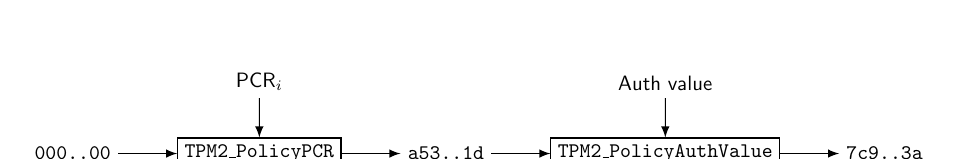
\begin{tikzpicture}[scale=.75, every node/.style={scale=.75}, node distance=3cm, font=\sffamily]
		\node[]                           (zerostart)   {\texttt{000..00}};
		\node[draw,right=.75cm of zerostart]    (policypcr)   {\texttt{TPM2\_PolicyPCR}};
		\node[right=.75cm of policypcr]         (authpol1)    {\texttt{a53..1d}};
		\node[draw,right=.75cm of authpol1] (policyauth)  {\texttt{TPM2\_PolicyAuthValue}};
		\node[right=.75cm of policyauth]        (authpol2)    {\texttt{7c9..3a}};
		
		\node[above=.5cm of policypcr]     (pcrs)        {$\text{PCR}_i$};
		\node[above=.5cm of policyauth]    (authval)     {Auth value};
		
		\draw[->] (zerostart) -- (policypcr);
		\draw[->] (policypcr) -- (authpol1);
		\draw[->] (authpol1) -- (policyauth);
		\draw[->] (policyauth) -- (authpol2);
		
		\draw[->] (pcrs) -- (policypcr);
		\draw[->] (authval) -- (policyauth);
	\end{tikzpicture}
	\caption{Calculation of the \texttt{authPolicy} for a key requiring both PCR values and a secret value, called the auth value}
	\label{fig:kappa-tpm2policy}
\end{figure}
When calculating the policy hash, the TPM first starts with an all-zero hash, then for each consecutive policy assertion the previous hash value is concatenated with the output from the policy function, and then hashed again as:
\begin{align}
	\text{policyDigest}^{\text{new}} = h(\text{policyDigest } || \text{ policyAssertionOutput})
\end{align}
similar to how the PCR values are updated in (\ref{eq:kappa-pcrextend}).
The output from the policy assertion is based on the provided parameters.
Using \texttt{TPM2\_PolicyPCR} as an example, the output will depend on the selection and values of PCRs.
When the TPM performs access control, it executes the policy assertions, and then compares the calculated hash with the value stored in the \texttt{authPolicy} field of the object.

Since the \texttt{authPolicy} is a hash value, we note that the order of the policy assertions is important.
Evaluating two policy assertions in a different order will result in a different hash value.
Chaining several policy assertions in sequence means that both assertions need to be valid for the authorization to be true, thus it can be seen as a logical AND.
To realize a logical OR, a separate policy command is required, \texttt{TPM2\_PolicyOR}.
This policy assertion is true if any of the previous branches is true.

\begin{figure}[htbp]
	\centering
	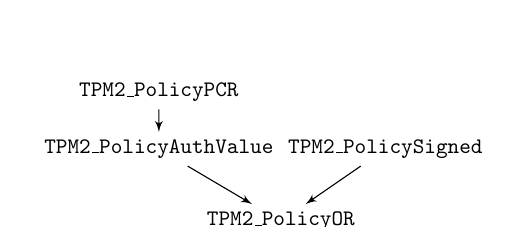
\begin{tikzpicture}[node distance=0.3cm,auto,>=latex',scale=0.8, every node/.style={scale=0.8}]
	\matrix (m) [matrix of nodes, row sep=0.3cm]
	{
		\texttt{TPM2\_PolicyPCR}       &                  &  \\
		\texttt{TPM2\_PolicyAuthValue} &                  & \texttt{TPM2\_PolicySigned} \\
		&                  & \\
	};
	\path (m-2-1) -- (m-2-3) node[midway] (m-2-2) {}; % helper node for placing the node below.
	\node[below=0.5cm of m-2-2] (m-3-2) {\texttt{TPM2\_PolicyOR}};
	
	\draw[->] (m-1-1) to (m-2-1);
	\draw[->] (m-2-1) to (m-3-2);

	\draw[->] (m-2-3) to (m-3-2);
	\end{tikzpicture}
	\caption{Example of a policy chain with \texttt{TPM2\_PolicyOR}}
	\label{fig:kappa-tpm2policystructure}
\end{figure}

Throughout this dissertation, we will describe policy chains using figures similar to Figure~\ref{fig:kappa-tpm2policystructure}.
The final hash value, stored in the object's \texttt{authPolicy}, is the result of the evaluation of the final (bottom) policy, thus the figures should be evaluated from top to bottom.
Using Figure~\ref{fig:kappa-tpm2policystructure} as an example, access to the object is granted if \emph{any} of the following two conditions are met:
\begin{enumerate}
	\item The PCR values match some desired values \emph{and} a correct authorization secret is given.
	\item A valid signature can be provided over some parameter.
\end{enumerate}
By combining logical AND and logical OR in this way, it is possible to construct a wide variety of policy assertions.

\subsection{Intel SGX}
\label{sec:kappa-sgx}

\newcommand{\sgxcommand}[1]{\texttt{#1}}
\newcommand{\sgxadd}{\sgxcommand{EADD}}
\newcommand{\sgxcreate}{\sgxcommand{ECREATE}}
\newcommand{\sgxenter}{\sgxcommand{EENTER}}
\newcommand{\sgxexit}{\sgxcommand{EEXIT}}
\newcommand{\sgxextend}{\sgxcommand{EEXTEND}}
\newcommand{\sgxgetkey}{\sgxcommand{EGETKEY}}
\newcommand{\sgxinit}{\sgxcommand{EINIT}}
\newcommand{\sgxremove}{\sgxcommand{EREMOVE}}
\newcommand{\sgxreport}{\sgxcommand{EREPORT}}
\newcommand{\sgxresume}{\sgxcommand{ERESUME}}
\newcommand{\sgxmrenclave}{\sgxcommand{MRENCLAVE}}
\newcommand{\sgxmrsigner}{\sgxcommand{MRSIGNER}}

Intel Software Guard Extensions (SGX) is a set of instructions built into modern CPUs produced by Intel.
Being a trusted computing technology, it provides several different security properties, including isolation, attestation, and sealing.
By providing the different security properties within the processor itself, it is now enough to trust only the CPU vendor.
This is opposed to for example the TPM, which requires trust in both the TPM vendor for attestation purposes, and the processor that executes the machine code.

The instruction set was first proposed in 2013, separately describing isolated execution \cite{mckeen:2013}, and attestation and sealing \cite{anati:2013}.
The first hardware with support for SGX was shipped in 2015, starting with Intel's Skylake architecture.

Since SGX is an extension of the instructions supported by the CPU, applications can use SGX specific instructions to use the various security properties.
The most central concept in SGX is the \emph{enclave}.
An enclave is a trusted execution environment (TEE) where code and data can be loaded at creation time.
After creation, the code can be measured for attestation purposes, and execution of the enclave is done in isolation, so that no other process or enclave on the system can read its memory.

SGX2 is an extension to the original SGX specification, which adds a set of extra instructions related to SGX memory and thread management.
The instructions are described in great detail in \cite{intel64b}, but are not discussed here, since SGX2 has not been used in this dissertation.

The life cycle of an enclave is described next, followed by the security properties, and their specific implementation and usage in SGX.

\subsubsection{Enclave Life Cycle}

An overview of the life cycle of an enclave can be seen in Figure~\ref{fig:kappa-lifeofenclave}.
The enclave is first created using \sgxcreate{}, which creates internal structures with metadata about the enclave.
This is followed by repeatedly calling \sgxadd{} for each 4~KiB page of memory to add to the enclave.
This copies memory from unprotected memory into the EPC of the enclave.
If desired, \sgxextend{} can be called to measure 256 bytes of memory of the enclave.
The measurement will be stored in a measurement log, which can later be used to attest the integrity of the enclave.
\sgxextend{} needs to be repeated for every 256 byte block that should be measured.

When all desired pages has been added to the enclave, \sgxinit{} should be called to finalize the creation stage.
After this, no more pages can be added to the enclave, and the measurement of the added pages will be finalized.

After initialization, the enclave code can be executed.
This is done by calling \sgxenter{}, which starts execution of enclave code at a predefined location.
The enclave then continues execution until either a controlled exit occurs using \sgxexit{}, or until an exception or interrupt occurs, which will be handled by AEX.
To avoid clutter, the AEX flow is not described in Figure~\ref{fig:kappa-lifeofenclave}, but after AEX, execution can be resumed in the enclave by issuing \sgxresume{}.

\begin{figure}[t]
	\centering
	\begin{tikzpicture}[scale=1, every node/.style={scale=1}, node distance=3cm,
	ibox/.style={draw,minimum width=2cm},
	stagebox/.style={dashed,gray,opacity=0.5}]
	\node[ibox]                        (create) {\sgxcreate};
	\node[ibox,right of=create]        (add)    {\sgxadd};
	\node[ibox,right of=add]           (extend) {\sgxextend};
	\node[ibox,right of=extend]        (init)   {\sgxinit};
	\node[ibox,below=1.5cm of create]  (enter)  {\sgxenter};
	\node[ibox,right of=enter]         (exit)   {\sgxexit};
	\node[ibox,below=1.5cm of enter]   (remove) {\sgxremove};
	
	\coordinate (createadd)  at ($(create)!0.5!(add)$);
	\coordinate (addextend)  at ($(add)!0.5!(extend)$);
	\coordinate (extendinit) at ($(extend)!0.5!(init)$);
	\coordinate (initenter)  at ($(init)!0.5!(enter)$);
	\coordinate (exitremove) at ($(exit)!0.5!(remove)$);
	\coordinate (removedone) at ([xshift=0.25cm,yshift=0.25cm]remove.north east);
	\coordinate[above=0.25cm of extendinit |- extend.north east] (abovepos1);
	\coordinate (abovepos2)  at ([xshift=0.25cm,yshift=0.25cm]exit.north east);
	
	\coordinate (createentera) at ($(create)!0.4!(enter)$);
	\coordinate (createenterb) at ($(create)!0.6!(enter)$);
	\coordinate (enterremovea) at ($(enter)!0.4!(remove)$);
	\coordinate (enterremoveb) at ($(enter)!0.6!(remove)$);
	
	\draw[->] (create) -- (add);
	\draw[->] (add) -- (extend);
	\draw[->] (extend) -- (init);
	\draw[->] (init) |- (initenter) -| (enter);
	\draw[->] (enter) -- (exit);
	\draw[->] (exit) |- (exitremove) -| (remove);
	
	\draw[->] ([xshift=-0.075cm]extendinit) |- (abovepos1 -| extend) -| (addextend);
	\draw[->] ([xshift=+0.075cm]extendinit) |- ([yshift=0.15cm]abovepos1) -| (createadd);
	
	\draw[->] (exit.east) -| (abovepos2) -| ([xshift=-0.25cm]enter.north east);
	\draw[->] (remove.east) -| (removedone) -| ([xshift=-0.25cm]remove.north east);
	
	%\draw[dashed,gray] (createenter -| create.west) -- (createenter -| init.east);
	\draw[stagebox] ([xshift=-0.75cm]createentera -| create.west) rectangle ([xshift=0.25cm,yshift=0.75cm]init.north east);
	\draw[stagebox] ([xshift=-0.75cm]enterremovea -| enter.west) rectangle ([xshift=0.25cm]createenterb -| init.north east);
	\draw[stagebox] ([xshift=-0.75cm,yshift=-0.5cm]remove.south west -| remove.west) rectangle ([xshift=0.25cm]enterremoveb -| init.north east);
	
	\node[gray,left=0.75cm of create.west,anchor=north,rotate=90] {\footnotesize creation};
	\node[gray,left=0.75cm of enter.west,anchor=north,rotate=90] {\footnotesize use};
	\node[gray,left=0.75cm of remove.west,anchor=north,rotate=90] {\footnotesize teardown};
	
	\end{tikzpicture}
	\caption{Overview of enclave life cycle with instructions used in the creation, use, and teardown stage}
	\label{fig:kappa-lifeofenclave}
\end{figure}

\subsubsection{Isolation}

Recall that isolation, or isolated execution, means that code and data are stored within an isolated environment.
An entity outside the isolated environment should not be able to read or modify data within the environment.
This section briefly describes the various means SGX has to provide isolation.
For a more in depth description, refer to \cite{mckeen:2013} and \cite{intel64b}.

An interesting property of SGX is that enclaves provide isolation from other processes on the system, the operating system, hypervisors, as well as other enclaves.
This allows several -- potentially mutually distrusting -- enclaves to coexist on the same system while still providing isolation guarantees.

A special area of the system memory, called the Enclave Page Cache (EPC), is used by enclaves to store data.
This area cannot be accessed by peripherals, other enclaves, or other parts of the system, including hypervisors or operating systems.
This is enforced by the memory controller in the CPU, which uses the Enclave Page Cache Map (EPCM) structure which stores information about each page in the EPC.
The EPCM is then used by the processor to make access control decisions when enclave memory is accessed.
The contents of the memory is also encrypted so that enclave data is never stored in DRAM in plaintext, since the CPU is the only trusted agent in the SGX model.

To maintain isolation of the enclave, the entry and exit of enclaves is controlled and done with the \sgxenter{} and \sgxexit{} instructions, respectively.
This also ensures that the enclave can only be entered at predefined locations.
In case of an interrupt or an exception, the enclave will save its state securely using a process called Asynchronous Enclave Exit (AEX).
AEX ensures that an exception or interrupt handler in an untrusted domain outside the enclave cannot gain access to the internal enclave state.

\subsubsection{Attestation}

An important part of SGX is the possibility to perform attestation of enclaves.
A key component of attestation is to first get a measurement of the code and data of the enclave.
There are two important measurement registers related to attestation in SGX, \sgxmrenclave{} and \sgxmrsigner{}.
Both registers are 256 bit wide, and store SHA-256 hashes.
\sgxmrsigner{} is a hash of the public key that has signed the enclave, thus identifying the author, while \sgxmrenclave{} stores the hash of code and data that is included during enclave creation, which will be described more in depth below.

\sgxmrenclave{} is calculated during the creation of an enclave during the addition of pages to the EPC occurring between \sgxcreate{} and \sgxinit{}.
The measurement calculation is shown in Figure~\ref{fig:kappa-mrenclavecalculation}.
\begin{figure}[ht]
	\centering
	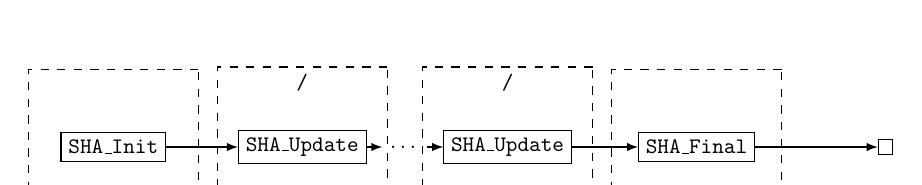
\begin{tikzpicture}[scale=0.8, every node/.style={scale=0.8}, node distance=3cm]
		\node[draw]                           (shainit)     {\texttt{SHA\_Init}};
		\node[draw,right of=shainit]          (shaupdate1)  {\texttt{SHA\_Update}};
		\node[     right=0.2cm of shaupdate1] (shaupdate2)  {\ldots};
		\node[draw,right=0.2cm of shaupdate2] (shaupdaten)  {\texttt{SHA\_Update}};
		\node[draw,right of=shaupdaten]       (shafinal)    {\texttt{SHA\_Final}};
		\node[draw,right of=shafinal]         (mrenclave)   {\sgxmrenclave{}};

		\draw[->] (shainit)    -- (shaupdate1);
		\draw[->] (shaupdate1) -- (shaupdate2);
		\draw[->] (shaupdate2) -- (shaupdaten);
		\draw[->] (shaupdaten) -- (shafinal);
		\draw[->] (shafinal)   -- (mrenclave);
		
		% dashed rectangles
		\node[draw,shape=rectangle,dashed,anchor=center,minimum width=2.7cm,minimum height=2cm] (shainitbox)    at (shainit.north)    {};
		\node[draw,shape=rectangle,dashed,anchor=center,minimum width=2.7cm,minimum height=2cm] (shaupdate1box) at (shaupdate1.north) {};
		\node[draw,shape=rectangle,dashed,anchor=center,minimum width=2.7cm,minimum height=2cm] (shaupdatenbox) at (shaupdaten.north) {};
		\node[draw,shape=rectangle,dashed,anchor=center,minimum width=2.7cm,minimum height=2cm] (shafinalbox)   at (shafinal.north)   {};
		
		\node[anchor=north] at (shainitbox.north)    {\sgxcreate{}};
		\node[anchor=north] at (shaupdate1box.north) {\sgxadd{}\texttt{/}\sgxextend{}};
		\node[anchor=north] at (shaupdatenbox.north) {\sgxadd{}\texttt{/}\sgxextend{}};
		\node[anchor=north] at (shafinalbox.north)   {\sgxinit{}};
	\end{tikzpicture}
	\caption{Overview of \sgxmrenclave{} derivation during enclave creation}
	\label{fig:kappa-mrenclavecalculation}
\end{figure}
The \sgxmrenclave{} measurement register is initialized during \sgxcreate{}.
Then, after each successive \sgxadd{} and \sgxextend{}, the hash is updated.
A call to \sgxadd{} will update the hash with metadata about the page that was added to the EPC, for example security properties, while a call to \sgxextend{} will update \sgxmrenclave{} with the content and metadata of a 256 byte data chunk.

SGX allows local attestation between enclaves on the same host, as well as remote attestation where an entity wishes to attest the integrity of an enclave running on a remote host.
This dissertation only considers the latter.
However, the local attestation sequence is relevant to understand how the remote attestation sequence works, thus both will be described below.

An overview of the local attestation flow can be found in Figure~\ref{fig:kappa-localsgxattestation}.
\begin{figure}[ht]
	\centering
	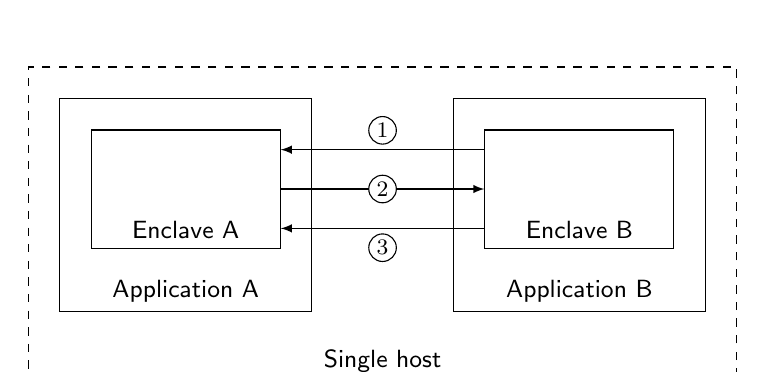
\begin{tikzpicture}[scale=1.0, every node/.style={scale=1.0}, node distance=3cm, font=\small\sffamily]
		\tikzset{circled/.style={draw,shape=circle,outer sep=2pt,inner sep=0.5pt,minimum size=0.35cm,font=\footnotesize,fill=white}}
		
		\node[draw,dashed,minimum width=9cm,minimum height=4cm] (userhost) {};
		
		\node[draw,solid,minimum width=3.2cm,minimum height=2.7cm,anchor=north west,below right=0.4cm and 0.4cm of userhost.north west] (appA) {};
		\node[draw,solid,minimum width=3.2cm,minimum height=2.7cm,anchor=north east,below left=0.4cm and 0.4cm of userhost.north east] (appB) {};
		
		\node[draw,solid,minimum width=2.4cm,minimum height=1.5cm,anchor=north,below=0.4cm of appA.north] (appAenclave) {};
		\node[draw,solid,minimum width=2.4cm,minimum height=1.5cm,anchor=north,below=0.4cm of appB.north] (appBenclave) {};
		
		\node[above=0.0cm of appA.south] {Application A};
		\node[above=0.0cm of appB.south] {Application B};
		
		\node[above=0.0cm of appAenclave.south] {Enclave A};
		\node[above=0.0cm of appBenclave.south] {Enclave B};
		
		\node[above=0.0cm of userhost.south] {Single host};
		
		\draw[<-] ([yshift=+0.5cm]appAenclave.east) -- node[above,circled] {1} ([yshift=+0.5cm]appBenclave.west);
		\draw[->] ([yshift=+0.0cm]appAenclave.east) -- node[      circled] {2} ([yshift=+0.0cm]appBenclave.west);
		\draw[<-] ([yshift=-0.5cm]appAenclave.east) -- node[below,circled] {3} ([yshift=-0.5cm]appBenclave.west);
	\end{tikzpicture}
	\caption{Overview of local attestation flow in SGX}
	\label{fig:kappa-localsgxattestation}
\end{figure}
The goal of the local attestation flow is for Enclave B to ensure that Enclave A is running on the same host as itself, that it is running inside an enclave, and that the expected code is running.
This is performed with the following steps \cite{anati:2013}:
\begin{enumerate}
	\item Enclave B sends its \sgxmrenclave{} value to Enclave A.
	\item Enclave A calls the \sgxreport{} instruction to generate a report structure, integrity protected using a MAC, containing data including \sgxmrenclave{} and \sgxmrsigner{}.
	The report is sent to Enclave B.
	Note that the key used to create this MAC is only known to Enclave B and the CPU itself, it is \emph{not} known by Enclave A.
	This proves that the report was created by trusted hardware, and not forged by Enclave A itself.
	\item Enclave B receives the report, and starts by verifying the MAC using its report key, retrieved by \sgxgetkey{}.
	If the MAC is valid, the contents of the report can be read, and Enclave B can verify the code and data integrity using \sgxmrenclave{} and \sgxmrsigner{}.
	If desired, Enclave B can now send its own report to Enclave A, if mutual attestation is desired.
\end{enumerate}

If we instead look at the remote attestation flow, a Verifier wishes to remotely attest an enclave running on a remote host.
An overview of the attestation sequence can be seen in Figure~\ref{fig:kappa-sgxattestation}.

\begin{figure}[ht]
	\centering
	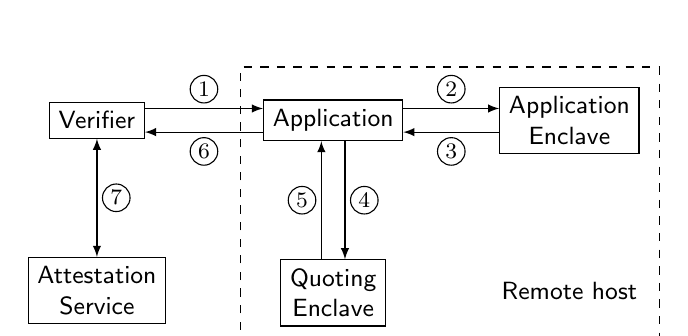
\begin{tikzpicture}[scale=1.0, every node/.style={scale=1.0}, node distance=3cm, font=\small\sffamily]
		\tikzset{circled/.style={draw,shape=circle,outer sep=2pt,inner sep=0.5pt,minimum size=0.35cm,font=\footnotesize}}

		\node[draw]                                         (verifier)     {Verifier};
		\node[draw,right of=verifier]                       (application)  {Application};
		\node[draw,right of=application,align=center]       (enclave)      {Application\\Enclave};
		\node[draw,below=1.5cm of application,align=center] (qe)           {Quoting\\Enclave};
		\node[draw,below=1.5cm of verifier,align=center]    (ias)          {Attestation\\Service};
		
		\draw[->] ([yshift=+0.15cm]verifier.east) -- node[above,circled] {1} ([yshift=+0.15cm]application.west);
		\draw[<-] ([yshift=-0.15cm]verifier.east) -- node[below,circled] {6} ([yshift=-0.15cm]application.west);
		
		\draw[->] ([yshift=+0.15cm]application.east) -- node[above,circled] {2} ([yshift=+0.15cm]enclave.west);
		\draw[<-] ([yshift=-0.15cm]application.east) -- node[below,circled] {3} ([yshift=-0.15cm]enclave.west);
		
		\draw[->] ([xshift=+0.15cm]application.south) -- node[right,circled] {4} ([xshift=+0.15cm]qe.north);
		\draw[<-] ([xshift=-0.15cm]application.south) -- node[left,circled]  {5} ([xshift=-0.15cm]qe.north);
		
		\draw[<->] (verifier.south) -- node[right,circled] {7} (ias.north);
		
		% dashed rectangle and label.
		\draw[dashed] ([xshift=0.25cm,yshift=0.25cm]enclave.north east) rectangle ([xshift=-0.5cm,yshift=-0.25cm]qe.south west);
		\node[below=1.5cm of enclave] (remotehost) {{Remote host}};
	\end{tikzpicture}
	\caption{Overview of remote attestation flow in SGX}
	\label{fig:kappa-sgxattestation}
\end{figure}

%\noindent
The numbered steps in the figure corresponds to the following steps in the attestation flow \cite{anati:2013}:
\begin{enumerate}
	\item The Verifier issues a challenge to the remote host, challenging it to prove that it runs code inside an enclave.
	\item The (untrusted) application forwards the challenge, together with the identity of the Quoting Enclave to the Application Enclave.
	The Quoting Enclave is an Intel-provided enclave.
	\item The Application Enclave calls the \sgxreport{} instruction to generate a report structure, integrity protected using a MAC, containing data such as \sgxmrenclave{} and \sgxmrsigner{}.
	The report is generated by the CPU, using a key only accessible to the CPU and the Quoting Enclave.
	The report is sent back to the application.
	\item The report is forwarded to the Quoting Enclave.
	\item The Quoting Enclave verifies the report by checking the MAC using its report key, retrieved by \sgxgetkey{}.
	If the MAC is valid, it creates a quote structure, containing the report and then signs the quote with a private platform-specific private key, using the EPID scheme \cite{brickell:2010}.
	Since this is a group signature scheme, it allows the creation of signatures without revealing the identity of the signing CPU.
	\item The signed quote is sent back to the Verifier.
	\item The Verifier can now verify the EPID signature of the quote by contacting an attestation service, typically the Intel Attestation Service (IAS), to ensure that the signature of the quote is valid. If it is, it can extract the \sgxmrenclave{} and \sgxmrsigner{} fields and compare them to known good values.
\end{enumerate}
After these steps, the Verifier can be sure that the enclave is: running inside an enclave on genuine hardware, and that the code and data in the enclave has not been modified before it was started.
These guarantees hold as long as the Verifier accepts the trust model of SGX.
Note that the communication between Application Enclave and Quoting Enclave is the local attestation flow described earlier, where the Quoting Enclave wishes to attest the Application Enclave.
Only if this local attestation is valid, the Quoting Enclave will sign the quote and pass it on.

For a more in depth description of attestation refer to \cite{anati:2013} and \cite{intel64b}.

\subsubsection{Sealing}

While the enclave protects the integrity and confidentiality of data while the enclave is running in memory, it can also be desirable to persist data to non-volatile media before the enclave exits.
This can be done by using sealing, which can be performed using several different policies in SGX.

Regardless of policy, the \sgxgetkey{} instruction is called together with the desired policy, and a 128-bit key is derived and returned by the CPU.
The key can then be used for encryption and/or integrity protection of data, before the data is persisted to disk.
Also, regardless of policy, the derived keys are unique to the particular CPU that derives the key; two identical enclaves running on different CPUs will derive different keys.
The sealing policies can be categorized into two major categories depending on the measurement register the key derivation is based on: either \sgxmrenclave{}-based or \sgxmrsigner{}-based.

In the first case, the sealing key will only be available to enclaves with the same \sgxmrenclave{} hash.
This ensures that only a particular enclave implementation will be able to unseal the data.
However, this also means that an updated version of the enclave, for example with security patches, will not be able to unseal data from a previous enclave version.

In the second case, the sealing key will be based on the \sgxmrsigner{} hash, together with a product id, and security version number (SVN).
The SVN can be used to allow an upgraded enclave to access sealed data from a previous version of the enclave.
This makes the management of security patches easier, since sealed data is accessible to newer enclave versions.
It is also possible to seal data without a product id, thus making it possible to share data between different enclaves from the same vendor.
For more details about sealing policies, refer to \cite{anati:2013} and \cite{intel64b}.

\subsubsection{Attacks on SGX}

Since the design of SGX was made public, there has been a progression in research related to potential attacks.

Several attacks have considered side-channel attacks related to memory management in Intel SGX, starting with the discussion of lack of protection against side-channel attacks in \cite{costan:2016}.
Fairly soon after these realizations, side-channel attacks on SGX started to appear.
In \cite{gotzfried:2017} the authors show a practical attack that can extract the AES key used for decryption inside an SGX enclave.
The attack is based on cache-timing attack, and can extract the AES key in less than 10 seconds, and is performed outside the enclave, thus breaking the isolation property of SGX.

Other attacks include \cite{schwarz:2017}, which performs an attack on an RSA implementation running within an enclave.
The attack is performed from within an attacker enclave, and attacks another enclave running on the same host.
It manages to recover the private RSA key either partially with a single trace, or completely when using multiple traces.
Similarly, \cite{brasser:2017} shows that the recovery of a private RSA key is possible, as well as the recovery of potentially sensitive genome data.
The extent of potential side-channel attacks is also discussed systematically in \cite{wang:2017}.

One way to avoid side-channel attacks is to implement algorithms in a data-oblivious way.
In \cite{ohrimenko:2016} this is discussed in the context of machine learning algorithms running inside SGX, where the authors propose data-oblivious algorithms for several common machine learning methods.
Also on the defensive side, \cite{gruss:2017} presents \emph{Cloak}, a technique to prevent attackers to observe cache misses.
The overall idea is to use hardware transactional memory, such as Intel TSX, which can be used to ensure that certain memory stays in the processor cache for the duration of the calculations, thus preventing cache-timing attacks.
The performance overhead is however heavily dependent on the amount of memory accesses in the code.

However, the previously mentioned mitigation does not always work.
In \cite{vanbulck:2018} the authors present Foreshadow, an attack based on the ideas from the Meltdown attacks \cite{lipp:2018}, but applied to SGX.
The attack leaks information from within the enclave, and also attacks the architectural enclaves such as the Quoting Enclave.

While the envisioned use case for SGX is to run trusted code within an enclave, shielding it from the unprotected world outside of SGX, \citeauthor{schwarz:2019} show that malware can be executed within an enclave \cite{schwarz:2019}.
Because of the isolation property of enclaves, such malware enclaves may avoid detection from anti-malware software running on the host.

%\cite{brasser:2017} % builds on others, easy to deploy, avoid detection rsa decryption, genomic processing
%\cite{gotzfried:2017} % 
%\cite{schwarz:2017}
%\cite{wang:2017} % considers many different sc in a systematic approach.
%\cite{gruss:2017}
%\cite{vanbulck:2018} % immune to gruss:2017 (cloak)
%\cite{schwarz:2019}

\subsection{Other Trusted Computing Technologies}
\label{sec:kappa-othertc}

While the previous sections have discussed trusted computing technologies used later on in this dissertation, it is also valuable to briefly discuss other potential options.
The main motivation behind this is that some contributions are not necessarily tied to a specific trusted computing technology, but could be implemented by using several others as well, as long as they provide the required combination of security properties.

One technology is Intel TXT, which allows the use of a DRTM for an execution environment \cite{TXT-mle}.
It allows for an application or operating system to launch a Measured Launch Environment (MLE) of trusted code.
Intel TXT uses the PCR values of the TPM to store measurements, together with new instructions to actually perform the launch of the MLE.

Related to the TPM, one variant of the TPM is the Mobile Trusted Module, based on the TPM 1.2 specification, but with adoptions for mobile use cases.
The specification can be seen in \cite{MTM1.0spec}, and for an overview of the functionality the reader is referred to \cite{ekberg:2007}.
There has been several proposed options for actual MTM implementations, for example implementations based on TrustZone (described next) \cite{winter:2008}, M-Shield \cite{ekberg:2009}, or as a physical chip \cite{kim:2010}.

Another technology is ARM TrustZone, available in ARM processors starting with ARMv6 in 2002 \cite{zhang:2016}.
TrustZone provides two different worlds: a secure world, and a normal world.
The normal world runs a regular, rich, operating system as well as all other regular software installed on the system.
The secure world typically runs a specialized trusted software stack, implementing the desired security features.
The processor ensures that software in the normal world cannot access memory of the secure world, while the secure world has access to all memory: both in the secure and normal world.

Other trusted computing technologies focus on other platforms, such as Sanctum \cite{costan:2016b} for RISC-V, SecureBlue++ \cite{boivie:2013} for POWER, and Bastion \cite{champagne:2010} for OpenSPARC.
For surveys of other technologies, we refer to for example \cite{zhang:2016,peters:2017,maene:2018}.

The different trusted computing technologies each provide a different API, and different ways to use the security properties they provide.
Ongoing efforts to abstract differences between different technologies include for example Asylo \cite{asylo} and Open Enclave \cite{openenclave}.

\subsection{Research on Trusted Computing}

With the previous sections describing the background of the various trusted computing technologies, this section describes research trends as well as potential applications of the technology.
Research on trusted computing covers a wide area, and can have applications both on client-oriented devices, as well as in more server-oriented use cases.

On client-oriented devices, BitLocker \cite{Bitlocker} is perhaps the most well-known use of the TPM today, being available in certain Windows versions since the launch of Windows Vista in 2007.
BitLocker is a disk encryption solution, and can use TPM sealing such that the disk encryption keys are only released when the boot environment is unmodified.

On mobile devices, where use of ARM processors is widespread, use of TrustZone is most common.
Examples include the use of TrustZone in the Android Keystore \cite{androidkeystore}, and Samsung Knox allowing containers, useful to, e.g., separate business and personal containers on a single device \cite{kanonov:2016}.
TrustZone can also be used as a trust root to implement other technologies.
An example is the Mobile Trusted Module which can be implemented by the use of TrustZone as a root as in \cite{winter:2008}.
While interesting, we will not consider such client-oriented applications further in this dissertation, and instead focus on more server-oriented use cases.
We first related to virtualization and cloud computing, followed by privacy-preserving measures.

\subsubsection{Virtualization and Cloud Computing}

There has been a lot of focus on the use of trusted computing technologies in the area of virtualization and cloud computing.
Starting with the TPM, which in itself is not trivially shared between multiple virtualized machines, \citeauthor{berger:2006} proposed virtualization of TPMs, vTPM, in \cite{berger:2006}, allowing virtual TPMs to be connected to virtual machines at the same time as trust in the vTPMs is rooted in the single hardware physical TPM.
Other approaches include para-virtualized TPM sharing \cite{england:2008}, and property-based TPM virtualization \cite{sadeghi:2008}.

A possible benefit of the cloud infrastructure is the possibility to increase availability.
Migrating services between different physical hosts allows flexibility of hardware maintenance, and is an import part of a cloud service.
However, migration introduces difficulties when combined with TPMs (both physical and virtualized), because of the underlying change in physical host.
The problems are discussed in papers such as \cite{danev:2011} and \cite{wan:2012}.

In \paperref{ch:tpmhas} we also consider the availability problem by describing the use of TPMs in a high-availability system (HAS).
Instead of a virtualization approach, we instead consider a system with multiple, independent, computational units (CUs) which together constitute the HAS.
We propose a solution for how each TPM-equipped CU can share the same keys required to decrypt secure storage for availability purposes, by describing a key migration scheme using the functionality in either TPM 1.2 or TPM 2.0.

In \paperref{ch:tpm12to20} the key migration features of both TPM versions are discussed in depth, as we design a way to migrate key material from TPM 1.2 to TPM 2.0, thus allowing the migration from old to new hardware while keeping the same keys.
Due to the lack of backwards compatibility between the two versions, this requires careful considerations to maintain the same key material and behaviour with regard to authorization.

Since SGX was presented in 2013, it has attracted much attention in virtualization and cloud computing.
Proposed use cases include distributed MapReduce computations while maintaining confidentiality and integrity \cite{schuster:2015}, shielded execution of applications in the cloud \cite{baumann:2015}, running Docker containers inside enclaves \cite{arnautov:2016}, and secure database engines \cite{priebe:2018}.

Network function virtualization (NFV) and Software-Defined Networking (SDN) are two technologies often used together with virtualization and in the cloud, since they allow an increased flexibility with regard to network management.
For an overview of respective technology, the reader is referred to \cite{casado:2014} and \cite{mijumbi:2016}. % first is for SDN, second for NFV + connection to SDN.
While security in SDN networks is a broad topic in itself, there has been previous research discussing trusted computing technologies in connection with SDN.
Examples include the discussions of securing inter-domain routing in \cite{kim:2015}, securing NFV states in \cite{shih:2016}, and a framework to securely bootstrap virtual network infrastructure in SDN \cite{paladi:2016b}.
In \paperref{ch:trustanchors} we also present contributions to the security in SDN networks, by presenting work protecting credentials and cryptographic context of network elements, as well as a secure enrollment mechanism for network elements in a software-defined network.
For both parts, we utilize trusted computing technologies.

\subsubsection{Privacy-preserving Computations}

The isolation guarantees of SGX are also interesting from a privacy-preserving perspective.
Performing privacy-preserving computations can be performed in many ways, including fully homomorphic encryption \cite{gentry:2009}, secure multiparty computation \cite{yao:1982}, and lastly by using trusted execution environments, which will be the focus of this section.

Privacy-related topics where SGX have been used are, e.g., a framework for MapReduce computations \cite{schuster:2015}, a sandbox to perform arbitrary calculations on secret data \cite{hunt:2018}, functional encryption \cite{fisch:2017}, multiparty computations \cite{kucuk:2016,bahmani:2017}, private web search \cite{mokhtar:2017,pires:2018}, and in machine-learning settings \cite{ohrimenko:2016,chandra:2017,hunt:2018b}.

In \paperref{ch:recsyssgx} we also use Intel SGX to design a privacy-preserving system, but in the context of a recommender system (recommender systems in general, and privacy in recommender systems in particular will be discussed shortly, in Section~\ref{sec:kappa-recommendersystems} and \ref{sec:kappa-recsysprivacy}, respectively).
In this recommender system, sensitive information consist of the user profiles, which are protected by designing an intermediary, running inside an SGX enclave.
The design using an intermediary is similar to the work presented in \cite{lie:2017}, where the intermediary is verifiable by the client before it is entrusted with sensitive information.
In contrast to our work, the targeted recommender system is different, where \paperref{ch:recsyssgx} considers a recommender which is not collaborative, which makes the use of validation predicates unnecessary -- malicious input would only affect the profile of the user itself.
Instead of blinding by combining multiple inputs, we derive pseudo profiles, used to issue fake queries together with the genuine query, similar to the approach discussed for private web search in \cite{mokhtar:2017}.

\newpage
\section{Recommender Systems}
\label{sec:kappa-recommendersystems}

The general goal of a recommender system is to provide recommendations from a set of items to some user, the idea being that the recommendations are adapted to the user's interests or needs.
Recommender systems are widely used in a lot of different scenarios, including e-commerce, music, videos, social media, and many others.
The common denominator is that there is a large set of content, such as books, songs, videos, or social media posts -- more than the user can or wishes to manually browse.
The purpose of a recommender is to filter this large set, which likely contains many items not relevant for the user, and present the filtered view to the user to further interact with.

The end goal of presenting this filtered view can be one of many, a few examples are listed below:
\begin{itemize}
	\item In an e-commerce setting, the goal is to increase the sales.
	By providing recommendations that the users are likely to be interested in, or at least likely to buy, the revenue of the seller can increase.
	\item For a monthly fixed-rate streaming service for music or videos, the goal may be to increase user satisfaction by providing recommendations of new or old content.
	\item For content financed with advertisements, the goal of the recommender could be to increase the ad revenue by recommending interesting content to the users, increasing the chance that they stay on the service and are exposed to more advertisements.
\end{itemize}

A conceptual view of a recommender system can be seen in Figure~\ref{fig:kappa-recommender}.
The recommender takes two inputs: user information and item information.

\begin{description}
	\item[User information] This can be any kind of information about a user, and the information can be supplied both explicitly and implicitly by the user.
	Examples of explicit user information would be user-stated preferences or properties such as interests, ratings, or age.
	Implicit user information could instead be automatically collected data about users, such as visited web pages, or purchase history.
	\item[Item information] This is instead information about the set of possible items to recommend.
	This is highly dependent on the items in question, but common examples are price, manufacturer, and product type, in case of a recommender system for manufactured goods.
\end{description}

\begin{figure}[tb]
	\centering
	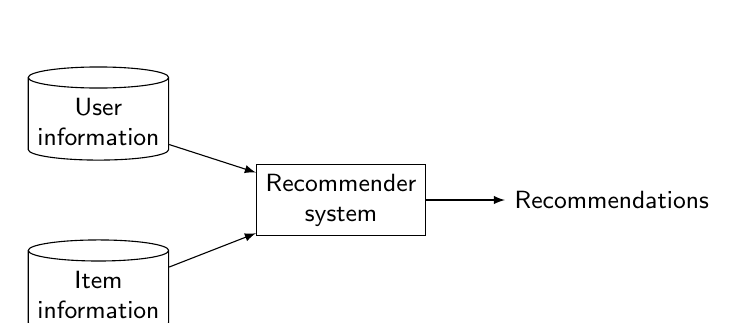
\begin{tikzpicture}[scale=1, every node/.style={scale=1}, node distance=1cm, font=\small\sffamily,
	database/.style={
		cylinder,
		shape border rotate=90,
		aspect=0.15,
		draw
	}],
		\node[draw,align=center]                             (recommender)     {Recommender\\system};
		\coordinate[left=2cm of recommender,anchor=east]     (midpoint);
		\node[database,above=0.5cm of midpoint,align=center] (userinfo)        {User\\information};
		\node[database,below=0.5cm of midpoint,align=center] (iteminfo)        {Item\\information};
		\node[right=of recommender]                          (recommendations) {Recommendations};
		
		\draw[->] (userinfo)    -- (recommender);
		\draw[->] (iteminfo)    -- (recommender);
		\draw[->] (recommender) -- (recommendations);
	\end{tikzpicture}
	\caption{Conceptual view of a recommender system}
	\label{fig:kappa-recommender}
\end{figure}

The recommender system combines user and item information, and outputs a set of recommendations, which is a subset or ranking of items that is likely to be relevant to the user in question.
The output can be of many forms, some common examples include:
\begin{itemize}
	\item A subset of all items, such that the subset contains items relevant to the user.
	\item A ranking of items, such that items are ordered according to their perceived relevance to the user.
\end{itemize}

Recommender systems can generally be categorized depending on the internal method used to generate the recommendations \cite{aggarwal:2016}.
Three major methods are: knowledge-based methods, content-based methods, and collaborative filtering methods.
They are described in more detail in the following sections.

\subsection{Knowledge-based Methods}

In a knowledge-based recommender system, the input of the recommender takes the form of user \emph{requirements} and item information, together with knowledge of the domain the recommender works in.
A distinctive feature of this type of recommender is that it does not work with user ratings or user history from previous interactions, but rather with a set of user-specified requirements.

There are two major classes of knowledge-based system, case-based and constraint based \cite{ricci:2011}. 
Case-based systems are based on a similarity function, which calculates the similarity between the desired item (user requirements), and items actually available.
Constructing the similarity function requires knowledge of the domain in question, but after construction it can be used to support several different interfaces.
The user can either specify individual requirements directly, or they can request items similar to other items.
Both interfaces are possible because they both use a similarity function.

The other class is constraint-based systems.
In these systems, the user typically provide their requirements in the form of constraints.
In case of a house or an apartment, it could be the minimum and maximum number of rooms, living area, etc.
The constraints do not have to explicitly map to item attributes; the designer of the recommender system can use domain-specific rules to map between user requirements and item attributes.
Compared to case-based systems above, the main difference lies in how case-based systems use a similarity function, while constraint-based systems use a set of rules that defines the mapping from requirements to items.

In general, knowledge-based systems are suitable in situations where items are bought rarely, such as cars, houses, apartments, and similar expensive items \cite{aggarwal:2016}.
In these cases, it can be hard to gather enough history of purchase to generate suitable recommendations.
Requirements may also change with time, consider the previous example of a recommender for real estate; it is very likely that the user's preferences have changed since the last time they bought a house or an apartment -- after all, there is a reason they are looking for something new.
Knowledge-based systems solve this by not trying to learn from past user behaviour, instead focusing on their current requirements, and use domain-specific knowledge to try to compare these requirements to item attributes.

\subsection{Content-based Methods}

Content-based methods take the individual history of the user into account when generating recommendations.
By considering the user's rating of previous items, the recommender tries to find similar items that the user may like.
This is done by comparing the attributes of previously liked items, and finding other items with similar attribute values.
A typical example is a movie recommender system, where a user has given a movie a high rank.
The recommender will then look at the attributes of the movie, and then try to find other movies with similar attributes, and presents these movies to the user.

Content-based systems have both advantages and disadvantages \cite{aggarwal:2016}.
Advantages include that newly added items can be recommended, since their attributes can be compared with older items immediately.
On the contrary, a well-known disadvantage is that new users cannot be given any reasonable recommendations, since they have not yet rated any item.
This is an example of the cold-start problem of recommender systems.

\subsection{Collaborative Filtering}

Collaborative filtering methods are typically designed around a rating matrix, such as the matrix in Figure~\ref{fig:kappa-cf}.
The rating matrix is sparse, and contains the ratings from a user $u_a$ of an item $i_b$.
Generating recommendations can now be seen as filling out this sparse matrix, such that unknown ratings are estimated by using data from other parts of the matrix.
An important distinction between collaborative filtering methods and previously described methods is that collaborative filtering also considers information from \emph{other} users of the system.

\begin{figure}[ht]
	\centering
	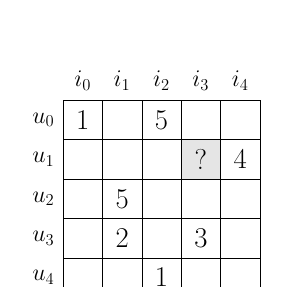
\begin{tikzpicture}[scale=0.5, every node/.style={scale=0.5}, node distance=1cm]
		\draw[step=1cm,very thin] (0, 0) grid (5, 5);
		
		\foreach \x in {0,...,4}
			\node at (\x+0.5, 5.5) {\LARGE $i_{\x}$};
		\foreach \y in {0,...,4}
			\node at (-0.5, 4-\y+0.5) {\LARGE $u_{\y}$};
		
		\draw[fill=gray!20] (3,3) rectangle (4,4);
		
		\foreach \x/\y/\v in {3/1/?, 1/2/5, 3/3/3, 0/0/1, 1/3/2, 4/1/4, 2/0/5, 2/4/1}
			\node[] at (\x+0.5, 4-\y+0.5) {\huge \v};
	\end{tikzpicture}
	\caption{Example of a rating matrix used in collaborative filtering}
	\label{fig:kappa-cf}
\end{figure}

Consider the rating matrix in Figure~\ref{fig:kappa-cf}.
The goal is to estimate the rating of some unknown $(u_a, i_b)$-pair in the rating matrix, for example the $(u_1, i_3)$-pair in Figure~\ref{fig:kappa-cf}, marked by the grey background.

A common methodology is to use neighbourhood-based collaborative filtering, which works by finding neighbourhoods of two different types.
A neighbourhood can either consist of similar users, or of similar items.
Again, using Figure~\ref{fig:kappa-cf} as an example, the former case corresponds to finding users with similar taste to $u_1$, and then finding \emph{their} ratings for the item $i_3$.
Thus, we look at ratings within the column $i_3$ from several users.
This is called user-based collaborative filtering, or user-user methods, and a more in-depth discussion can be found in \cite{herlocker:1999}.

The latter case, finding items that are similar to $i_3$, instead corresponds to looking at ratings on the same row, for those items that are similar to $i_3$.
This is called item-based collaborative filter, or item-item methods.
One advantage of item-item methods is that the relations between items are less likely to change, as opposed to user-user relations.
This can be used for performance optimizations, since the online-phase of computations can be reduced \cite{sarwar:2001}.

\subsection{Construction of Recommender Systems}

In this section, some aspects the construction of recommender systems are discussed.
We start by discussing similarity and utility functions, and how they are used in the different recommender system methods.
We then discuss how several recommender system methods can be combined together -- creating hybrid recommender systems.

\subsubsection{Similarity and Utility Functions}

A concept used in several of the previously mentioned recommender methods is similarity and utility functions.
At first, a discussion and definition of the two kind of functions are required; the definitions will then be used throughout the rest of this dissertation.
This is followed by examples of different similarity functions.

As the name implies, similarity functions are used to measure the similarity between two values.
In the general case, a similarity function can be defined in two ways: as the similarity between two users or items as a whole, or between two individual attribute values.
\begin{figure}[ht]
	\begin{subfigure}[b]{0.5\linewidth}
		\centering
		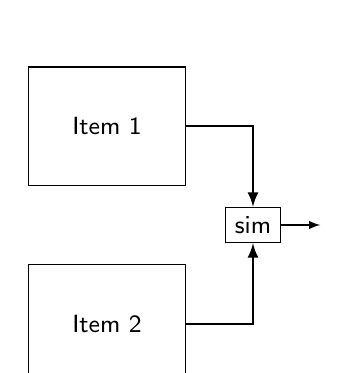
\begin{tikzpicture}[scale=1, every node/.style={scale=1}, node distance=1.0cm, font=\small\sffamily,
		item/.style={minimum width=2cm, minimum height=1.5cm,draw}]
		\node[item]                (item1) {Item 1};
		\node[item,below=of item1] (item2) {Item 2};
		\coordinate (item15) at ($(item1)!0.5!(item2)$) {};

		\node[draw,right=1.5cm of item15,align=center] (sim) {\textsf{sim}};

		\draw[->,thick] (item1) -| (sim);
		\draw[->,thick] (item2) -| (sim);
		\draw[->] (sim.east) -- +(0.5cm,0);
		\end{tikzpicture}
%		\captionsetup{singlelinecheck=true}
		\caption{Between two items}
		\label{fig:kappa-simlargevsattributelarge}
	\end{subfigure}
	\begin{subfigure}[b]{0.5\linewidth}
		\centering
		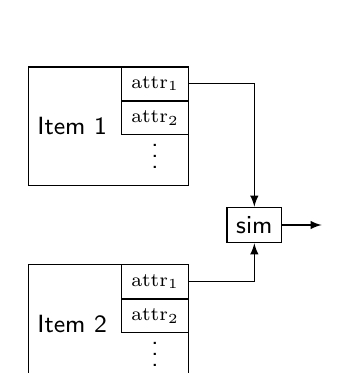
\begin{tikzpicture}[scale=1, every node/.style={scale=1}, node distance=1.0cm, font=\small\sffamily,
		item/.style={anchor=west,minimum width=2cm, minimum height=1.5cm,text width=1.8cm,draw},
		attr/.style={anchor=north east,minimum width=0.85cm,minimum height=0.375cm,draw,font=\scriptsize}]
		\node[item]                (item1) {Item 1};
		\node[item,below=of item1] (item2) {Item 2};
		\coordinate (item15) at ($(item1)!0.5!(item2)$) {};

		% attributes		
		\node[attr] (i1a1) at (item1.north east) {$\text{attr}_1$};
		\node[attr,below=0cm of i1a1] (i1a2)     {$\text{attr}_2$};
		\node[anchor=north east,below=-0.1cm of i1a2,inner sep=0] (i1a3) {\vdots};
		
		\node[attr] (i2a1) at (item2.north east) {$\text{attr}_1$};
		\node[attr,below=0cm of i2a1] (i2a2)     {$\text{attr}_2$};
		\node[anchor=north east,below=-0.1cm of i2a2,inner sep=0] (i2a3) {\vdots};

		% sim func and arrows	
		\node[draw,right=1.5cm of item15,align=center] (sim) {\textsf{sim}};
		
		\draw[->] (i1a1) -| (sim);
		\draw[->] (i2a1) -| (sim);
		\draw[->] (sim.east) -- +(0.5cm,0);
		\end{tikzpicture}
%		\captionsetup{singlelinecheck=true}
		\caption{Between individual attributes}
		\label{fig:kappa-simlargevsattributeattribute}
	\end{subfigure}
	\caption{Two ways to define similarity functions (\textsf{sim})}
	\label{fig:kappa-simlargevsattribute}
\end{figure}
The distinction is visualized in Figure~\ref{fig:kappa-simlargevsattribute}, where \figref{fig:kappa-simlargevsattributelarge} shows the case where the similarity function takes two complete items as input, and outputs a similarity metric.
In \figref{fig:kappa-simlargevsattributeattribute} the similarity function is instead defined between individual attributes.
Also, while the figures show items and item attributes, note that it is also possible to use users and user attributes instead.
Depending on the recommender type, it may also be applicable for the similarity function to be defined between an item and a user.
This is the case for knowledge-based recommender systems, where user requirements and item attributes are compared using a similarity function.

Utility functions can be defined in the same way as similarity functions, but as the naming suggests, they are often used to give a more general metric of \emph{utility}, as opposed to just similarity.
Consider the example in Figure~\ref{fig:kappa-simvsutility}, where the user requirements for a computer are compared to two different items.
\begin{figure}[ht]
	\centering
	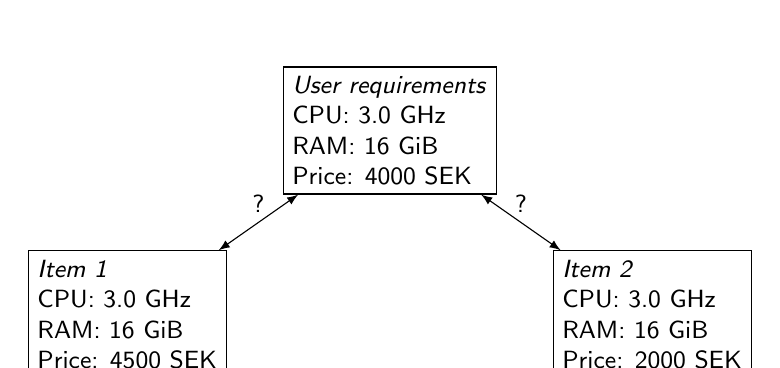
\begin{tikzpicture}[scale=1.0, every node/.style={scale=1.0}, node distance=1cm, font=\small\sffamily]
	\node[draw,align=left] (req) {\emph{User requirements}\\CPU: 3.0 GHz\\RAM: 16 GiB\\Price: 4000 SEK};
	
	\node[draw,align=left,below left=of req]  (item1) {\emph{Item 1}\\CPU: 3.0 GHz\\RAM: 16 GiB\\Price: 4500 SEK};
	\node[draw,align=left,below right=of req] (item2) {\emph{Item 2}\\CPU: 3.0 GHz\\RAM: 16 GiB\\Price: 2000 SEK};
	
	\draw[<->] (req) -- node[above] {?} (item1);
	\draw[<->] (req) -- node[above] {?} (item2);
	
	\end{tikzpicture}
	\caption{User requirements being compared with two different items}
	\label{fig:kappa-simvsutility}
\end{figure}
Assuming CPU, RAM, and price being the only possible attributes of a computer, which of the two items matches best with the user requirements?
If a strict definition of similarity is used, clearly the more expensive Item 1 is more similar to the user requirements; the desired price of 4000 SEK is clearly closer to 4500 SEK than to 2000 SEK.
While mathematically sound, this is most probably not the desired behaviour from a user perspective; clearly, if the user can get the same specifications to a lower price, that is more desirable.
Therefore, it is reasonable to say that Item 2 has a higher utility than Item 1.
Utility metrics are highly dependent on the domain in which they are used, while a lower price is generally more desirable than a higher price, the opposite may be true for other attributes.
However, the distinction between similarity and utility can sometimes be unclear, and the notation varies between different contexts.

After these generic descriptions, we now move on to the definitions used in the remainder of this dissertation.
With the regard to similarity and utility functions, the following notation will be used:
\begin{itemize}
	\item Similarity functions will compare \emph{individual attributes}.
	Attributes can be both user attributes, and item attributes.
	For consistency, the term \emph{similarity function} will be used both when comparisons are done based on similarity, or based on a metric that could be considered more utility-based.
	\item Utility functions will be used to describe the utility of a \emph{complete item} for a specific user.
	To calculate the utility, it will apply similarity functions to the individual attributes, and combine the similarities to derive a utility metric.
\end{itemize}
The use is visualized in Figure~\ref{fig:kappa-simutilitydefs}.
\begin{figure}[htb]
	\centering
	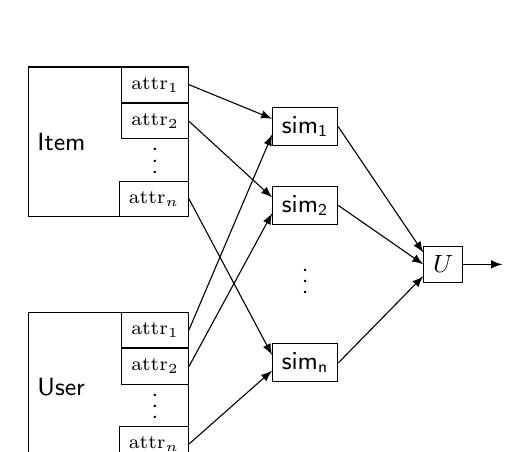
\begin{tikzpicture}[scale=1, every node/.style={scale=1}, node distance=1.2cm, font=\small\sffamily,
		item/.style={anchor=west,minimum width=2cm, minimum height=1.9cm,text width=1.8cm,draw},
		attr/.style={anchor=north east,minimum width=0.85cm,minimum height=0.45cm,draw,font=\scriptsize}]

		\node[item]                (item1) {Item};
		\node[item,below=of item1] (user1) {User};
		\coordinate (itemuser) at ($(item1)!0.5!(user1)$);
		\coordinate[right=2.5cm of itemuser] (simmiddle);

		% attributes		
		\node[attr] at (item1.north east)                          (i1a1) {$\text{attr}_1$};
		\node[attr,below=0cm of i1a1]                              (i1a2) {$\text{attr}_2$};
		\node[anchor=north east,below=-0.1cm of i1a2,inner sep=0]  (i1a3) {\vdots};
		\node[attr,anchor=south east] at (item1.south east)        (i1a4) {$\text{attr}_n$};

		\node[attr] at (user1.north east)                         (u1a1) {$\text{attr}_1$};
		\node[attr,below=0cm of u1a1]                             (u1a2) {$\text{attr}_2$};
		\node[anchor=north east,below=-0.1cm of u1a2,inner sep=0] (u1a3) {\vdots};
		\node[attr,anchor=south east] at (user1.south east)       (u1a4) {$\text{attr}_n$};

		% sim func and arrows	
		\node[draw,above=1.5cm of simmiddle] (sim1) {$\mathsf{sim_1}$};
		\draw[->] (i1a1.east) -- ([yshift=+0.1cm]sim1.west);
		\draw[->] (u1a1.east) -- ([yshift=-0.1cm]sim1.west);

		\node[draw,above=0.5cm of simmiddle] (sim2) {$\mathsf{sim_2}$};
		\draw[->] (i1a2.east) -- ([yshift=+0.1cm]sim2.west);
		\draw[->] (u1a2.east) -- ([yshift=-0.1cm]sim2.west);

		\node[above=-0.5cm of simmiddle] (simdots) {\vdots};

		\node[draw,above=-1.5cm of simmiddle] (simn) {$\mathsf{sim_n}$};
		\draw[->] (i1a4.east) -- ([yshift=+0.1cm]simn.west);
		\draw[->] (u1a4.east) -- ([yshift=-0.1cm]simn.west);

		% utility func and arrows
		\node[draw,right=1.5cm of simmiddle] (utility) {$U$};
		\draw[->] (sim1.east) -- ([yshift=+0.15cm]utility.west);
		\draw[->] (sim2.east) -- ([yshift=+0.00cm]utility.west);
		\draw[->] (simn.east) -- ([yshift=-0.15cm]utility.west);
		\draw[->] (utility.east) -- +(0.5cm,0);
	\end{tikzpicture}
	\caption{Use of similarity (\textsf{sim}) on attributes, and utility ($U$) functions to combine the results, which will be used later in this dissertation}
	\label{fig:kappa-simutilitydefs}
\end{figure}

As mentioned earlier, and using the definitions above, similarity functions need to be defined  differently depending on the attributes they are used for.
In general, we define a similarity function to take two attributes, one item attribute value $v$ and one user attribute value called the \emph{target} value $t$.
The output of the similarity function is a value between $0$ and $1$, and a higher value means a higher similarity.
Thus, more formally, for all similarity functions we have
\begin{align}
	0 \le \mathsf{sim}(t, v) \le 1 \,.
\end{align}

\paragraph{Examples of Similarity Functions}
A straightforward example of a similarity function is the distance function $\mathsf{sim_\text{dist}}$, which returns $1$ if the value $v$ is equal to target $t$, and otherwise decreases linearly toward $0$ as the difference between $v$ and $t$ increases.
\begin{align}
	\mathsf{sim_\text{dist}}(t, v) = 1 - \frac{|t - v|}{\max_\text{dist} - \min_\text{dist}} \,,
\end{align}
where $\max_\text{dist}$ and $\min_\text{dist}$ are the maximum and minimum possible distances between $t$ and $v$.
This scaling ensures that the output is between $0$ and $1$.
For an example of plot for some values, see Figure~\ref{fig:kappa-simdistplot}.

While $\mathsf{sim_\text{dist}}$ is an example of a symmetric similarity function (it is mirrored around $v=t$), similarity functions can also be defined in many other ways.
Asymmetric function can be useful in instances when the similarity metric should not penalize values above the target value.
Looking back at the computer component example earlier, a computer with more RAM or faster CPU than the target value should not be penalized.
This can be realized using a similarity function such as
\begin{align}
	\mathsf{sim}_\text{asym}(t, v) =
	\begin{cases}
		1 - \frac{|t - v|}{\max_\text{dist} - \min_\text{dist}} & \text{if } v < t \\
		1                                                       & \text{if } v \ge t
	\end{cases} \,,
\end{align}
which is also plotted in Figure~\ref{fig:kappa-simasymplot}.

Another useful example is a scoring function, where the target value $t$ is not a target value \emph{per se}, but rather a form of weight.
\begin{align}
	\mathsf{sim_\text{score}}(t, v) = t \cdot v
\end{align}
It is particularly simple to use if $ v \in [0,1]$, since the target value can then simply be selected such that $t \in [0,1]$ as well, guaranteeing the output to be in the range $[0,1]$ as well.
A plot can be seen in Figure~\ref{fig:kappa-simscoreplot}.

\begin{figure}[ht]
	\captionsetup{singlelinecheck=true}
	\begin{subfigure}[b]{0.33\linewidth}
		\centering
		\resizebox{\linewidth}{!}{
		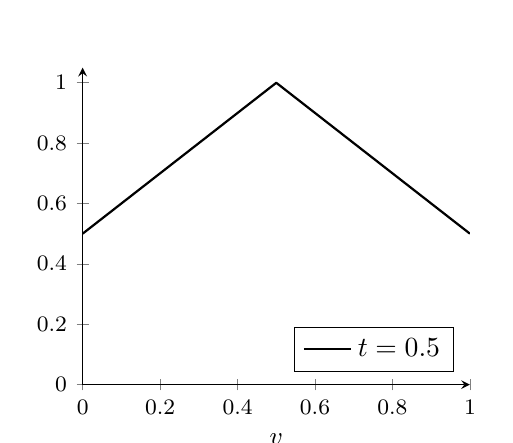
\begin{tikzpicture}
			\pgfplotsset{every axis legend/.append style={at={(0.96,0.04)},anchor=south east}}
			\begin{axis}[small,xlabel=$v$,xmin=0,xmax=1.0,ymin=0.0,ymax=1.05,axis lines=left]
				\addplot[thick,black,domain=0.0:1.0,samples=500]
					{ 1.0 - abs(0.5 - x)/1.0
};
				\addlegendentry{$t=0.5$}
			\end{axis}
		\end{tikzpicture}
		}
		\caption{$\mathsf{sim_\text{dist}}$}
		\label{fig:kappa-simdistplot}
	\end{subfigure}%
	\begin{subfigure}[b]{0.33\linewidth}
		\centering
		\resizebox{\linewidth}{!}{
		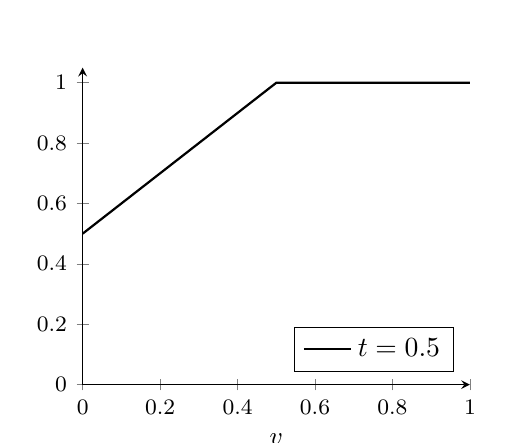
\begin{tikzpicture}
			\pgfplotsset{every axis legend/.append style={at={(0.96,0.04)},anchor=south east}}
			\begin{axis}[small,xlabel=$v$,xmin=0,xmax=1.0,ymin=0.0,ymax=1.05,axis lines=left]
				\addplot[thick,black]
					coordinates {
						(0.0,0.5)
						(0.5,1.0)
						(1.0,1.0)
					};
			\addlegendentry{$t=0.5$}
			\end{axis}
		\end{tikzpicture}
		}
		\caption{$\mathsf{sim_\text{asym}}$}
		\label{fig:kappa-simasymplot}
	\end{subfigure}%
	\begin{subfigure}[b]{0.33\linewidth}
		\centering
		\resizebox{\linewidth}{!}{
		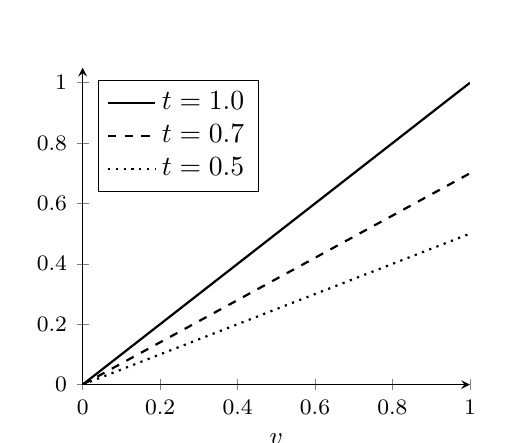
\begin{tikzpicture}
			\pgfplotsset{every axis legend/.append style={at={(0.04,0.96)},anchor=north west}}
			\begin{axis}[small,xlabel=$v$,xmin=0,xmax=1.0,ymin=0.0,ymax=1.05,axis lines=left]
				\addplot[thick,black,domain=0.0:1.0,samples=500]
					{ 1.0 * x
};
				\addlegendentry{$t=1.0$}
				\addplot[dashed,thick,black,domain=0.0:1.0,samples=500]
					{ 0.7 * x
};
	
				\addlegendentry{$t=0.7$}
				\addplot[dotted,thick,black,domain=0.0:1.0,samples=500]
					{ 0.5 * x
};
				\addlegendentry{$t=0.5$}
			\end{axis}
		\end{tikzpicture}
		}
		\caption{$\mathsf{sim_\text{score}}$}
		\label{fig:kappa-simscoreplot}
	\end{subfigure}%
	\caption{Similarity metrics plotted as a function of the value $v$, for different similarity functions. The y-axis is the output from the similarity function, the target value $t$ is given in the legend of each line.}
	\label{fig:kappa-similarityfunctions}
\end{figure}

\subsubsection{Hybrid Recommender Systems}
\label{sec:kappa-hybridrecommenders}

Each of the three classes of recommender systems mentioned before has their own advantages and disadvantages.
Knowledge-based systems works well in a cold-start setting, but does not consider user history.
Content-based systems works well when new items are added, but fails to present recommendations for new users.
Collaborative filtering methods can utilize ratings from other users, but may not work well if the rating matrix is too sparse.

The idea of hybrid recommenders is to combine several recommender methods, such that they do not run in isolation, but rather together with other methods.
This allows the hybrid recommender to benefit from the advantages of the individual recommender methods, and hopefully avoid the disadvantages.

Hybrid recommenders can be constructed in various ways, depending on how the different subsystems are interconnected, what input each subsystem has, and how the output is constructed.
Examples of constructions as well a classifications are described in \cite{burke:2002}, however, we will only focus on one particular construction, which is described next.

One straightforward way to construct a hybrid recommender is to construct a \emph{weighted} hybrid, which has a layout as in Figure~\ref{fig:kappa-weightedhybrid}.
Each subsystem has the same input, and the output is then calculated as a weighted average where each individual subsystem has a certain weight $w_i$.
We will later return to this type of hybrid recommender when we construct a recommender system in \paperref{ch:recsys}.

\begin{figure}[th]
	\centering
	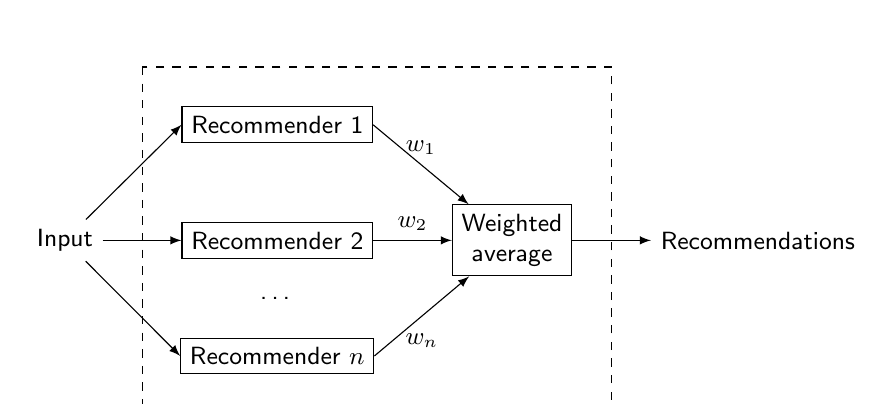
\begin{tikzpicture}[scale=1, every node/.style={scale=1}, node distance=1cm, font=\small\sffamily]
		\node[draw]                       (recommender1) {Recommender 1};
		\node[draw,below=of recommender1] (recommender2) {Recommender 2};
		\node[draw,below=of recommender2] (recommendern) {Recommender $n$};
		\node[] at ($(recommender2)!0.5!(recommendern)$) {\ldots};
		
		\node[draw,right=of recommender2,align=center] (combiner) {Weighted\\average};
		
		\node[left=of recommender2]  (input)           {Input};
		\node[right=of combiner]     (recommendations) {Recommendations};
		
		\coordinate (recommendernshifted) at ([yshift=-0.5cm]recommendern.south east);
		\draw[dashed] ([xshift=-0.5cm,yshift=+0.5cm]recommender1.north west) rectangle ([xshift=+0.5cm]combiner.east |- recommendernshifted);
		
		\draw[->] (input) -- (recommender1.west);
		\draw[->] (input) -- (recommender2.west);
		\draw[->] (input) -- (recommendern.west);
		
		\draw[->] (recommender1.east) -- node[above] {$w_1$} (combiner);
		\draw[->] (recommender2.east) -- node[above] {$w_2$} (combiner);
		\draw[->] (recommendern.east) -- node[below,outer sep=3pt] {$w_n$} (combiner);
		
		\draw[->] (combiner) -- (recommendations);
	\end{tikzpicture}
	\caption{Overview of a weighted recommender system}
	\label{fig:kappa-weightedhybrid}
\end{figure}

\subsection{Research on Recommender Systems}
% was Recommender Systems in Software Security

Research in recommender systems can be made in several different ways.
Focus can be on presenting new or refined algorithms for the various recommender methods, as well as introducing new use cases of recommender systems.

Significant advances, specifically in the area of collaborative filtering, have been made during the course of the Netflix Prize \cite{netflixprize}.
The competition, organized by the media-services provider Netflix, took place from October 2006 until the winning team was announced in September 2009.
The prize awarded to the winner was 1 million US dollars, if the accuracy of the designed solution beat Netflix's own recommender Cinematch by 10\%.
Together with the announcement of the competition, Netflix also published a large dataset of anonymized user rankings useful for training recommenders.
The winning recommender, named ``BellKor's Pragmatic Chaos'', from the combination of solutions from three different teams, finally achieved an improvement of 10.06\%.
The design is described in three separate papers \cite{koren:2009,toscher:2009,piotte:2009}.
For other contributions related to the prize refer to, e.g., \cite{zhou:2008,takacs:2008} for some examples of systems using the anonymized dataset.

Research is also focused on applying recommender systems in new areas to find use~cases that have not yet seen the potential benefits of recommender systems.
Some examples of use~cases for recommenders include movie recommendations \cite{diao:2014,harper:2015}, e-commerce \cite{huang:2007,castroschez:2011}, music \cite{schedl:2015,kaminskas:2013}, web services \cite{zheng:2009}, or research articles \cite{wang:2018}.

In this dissertation, we consider the application of recommender systems in the cyber security domain.
The subject of cyber security is wide, and recommender systems have been proposed to several different areas.
Previous work in the area includes the use or recommender systems to
recommend cyber defence actions to cyber warriors \cite{lyons:2014},
detect unsafe coding practices and suggest fixes in Java source code \cite{nembhard:2019},
and predict attacks in a network using a graph of attack paths \cite{polatidis:2017}.

More specifically, the use of recommender systems can also be applied to the area of software vulnerability management.
As new software vulnerabilities are discovered, it is increasingly important for software vendors to discover, analyse, and handle them.
Vulnerabilities can arise both in code developed by the vendors themselves, but can also be discovered in third-party libraries included in the software package.
Using a recommender system to aid in various parts of the vulnerability management life cycle has been proposed in earlier work.
In \cite{farris:2018} the authors propose a recommender system to reduce time-to-vulnerability remediation as well as total vulnerability exposure within an organization.
Others have instead looked at using recommender systems to propose actions to take after discovering a vulnerability \cite{gadepally:2016}.
Text-mining is used in \cite{lee:2018} to find vulnerabilities related to each other, which is then used to construct a vulnerability ranking.

In \paperref{ch:recsys} we also construct a recommender system for vulnerabilities.
Our recommender is based on a hybrid approach (see Section~\ref{sec:kappa-hybridrecommenders}) and the goal is to produce a user-specific vulnerability scoring.
This is in contrast to common vulnerability scoring methods such as CVSS \cite{cvss2spec,cvss3spec} used by NVD \cite{nvd} to provide a non-individualized vulnerability score.
This recommendations are generated by combining traits from two of the previously mentioned recommender types, knowledge-based, and content-based, combined with domain-specific knowledge of the field of software vulnerabilities.

\subsection{Privacy in Recommender Systems}
\label{sec:kappa-recsysprivacy}

After discussing how recommenders can be used to aid in software security, we now turn the focus to security of the recommender systems themselves.
For recommenders to provide useful output to users, they clearly must store and process information about every user of the system.
Such data collection gives rise to privacy concerns, since the data can be used to build an intimate profile of a user's interests, opinions, identity, or other personal information, depending on the type of recommender.

Earlier research has shown that the privacy risks of recommenders exists in real life.
In \cite{narayanan:2008}, the authors present a de-anonymization attack on the Netflix Prize dataset.
While anonymization techniques had been applied to the dataset before being published by Netflix, the authors show that with knowledge of some information about a user, their full record can be identified in the dataset.
Applied to the Netflix dataset, this means that knowing some information about a user's previously watched or rated movies, could allow an attacker to gain information about all movies the user has watched or rated.

By using differential privacy \cite{dwork:2006}, the authors of \cite{mcsherry:2009} present a design that builds privacy into recommender systems.
They apply differential privacy to the recommenders, while still maintaining a high accuracy despite the introduced noise.

Potential privacy risks of collaborative filtering are also discussed in \cite{calandrino:2011}, where the authors present inference attacks to get customer data by observing public output from recommender system.
Such risks are also one reason why collaborative filtering methods are avoided in some settings, for example in the recommender system presented in \paperref{ch:recsys} of this dissertation.
Privacy-preserving methods for collaborative filtering tries to solve this, but are not covered further in this dissertation, instead we refer to previous work in the area, e.g., \cite{zhan:2010,polat:2003,canny:2002,parameswaran:2007,polat:2005}.

In this dissertation, \paperref{ch:recsyssgx} presents a privacy-preserving system to provide recommendations for software vulnerabilities.
The user profiles contain sensitive information, since they can provide an observer with information about internal vulnerability management processes of the user.
By using trusted computing, specifically Intel SGX (see Section~\ref{sec:kappa-sgx}), and k-anonymity \cite{samarati:1998,samarati:2001}, we propose a solution that preserves the privacy of the user profiles, without requiring modification of the recommender system itself.

\newpage
\section{Cryptography}
\label{sec:kappa-cryptography}

The area of cryptography covers a wide range of different functionality, e.g., making messages unreadable to unauthorized parties, ensuring that they have not been modified during transfer, and creating digital signatures to provide proof of authenticity.
The different algorithms that provide this functionality can be classified into different categories, called cryptographic primitives.
Common cryptographic primitives include one-way hash functions, symmetric encryption algorithms, public-key encryption algorithms, and digital signatures.
Such primitives are commonly combined into cryptographic protocols, which provide a richer set of features.
An example of such a protocol is Transport Layer Security (TLS) \cite{rfc8446}, which provides a secure channel with confidentiality, integrity, and authentication.
TLS achieves this by combining cryptographic primitives such as encryption algorithms, and key exchange protocols.

The purpose of encryption algorithms -- commonly called \emph{ciphers} -- is to conceal messages such that they are unintelligible to an unauthorized party.
Only an authorized party can reverse the steps of the encryption -- called decryption -- and retrieve the original message.
An overview of the process can be seen in Figure~\ref{fig:kappa-encdec}.
A message $m$, also called \emph{plaintext}, is sent into the encryption algorithm together with a key $K_e$.
The resulting encrypted message $c$, called \emph{ciphertext}, is the result from this encryption step.
On the receiver's end, the ciphertext is fed into the decryption algorithm, together with a key $K_d$.
The output from the decryption is the original message $m$.
This description is very general, and applicable to ciphers in general.

\begin{figure}[ht]
	\centering
	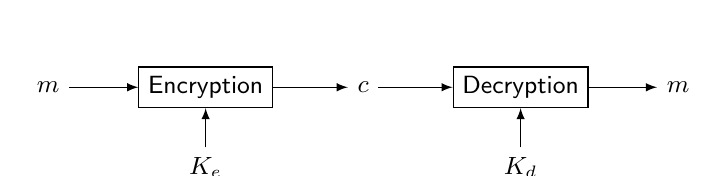
\begin{tikzpicture}[scale=1, every node/.style={scale=1}, node distance=2cm, font=\small\sffamily]
		\node[draw]                (encryption)  {Encryption};
		\node[left of=encryption]  (plaintext)   {$m$};
		\node[right of=encryption] (ciphertext)  {$c$};
		\node[below=0.5cm of encryption] (key-e) {$K_e$};
		
		\draw[->] (plaintext.east) -- (encryption.west);
		\draw[->] (encryption.east) -- (ciphertext.west);
		\draw[->] (key-e.north) -- (encryption.south);

		\node[right of=ciphertext,draw]  (decryption)   {Decryption};
		\node[right of=decryption]        (plaintext2)   {$m$};
		\node[below=0.5cm of decryption] (key-d)        {$K_d$};
		
		\draw[->] (ciphertext.east) -- (decryption.west);
		\draw[->] (decryption.east) -- (plaintext2.west);
		\draw[->] (key-d.north) -- (decryption.south);
	\end{tikzpicture}
	\caption{Overview of encryption and decryption flow}
	\label{fig:kappa-encdec}
\end{figure}

Ciphers can be divided into two categories, depending on how the keys $K_e$ and $K_d$ are related.
In asymmetric ciphers, or public-key ciphers, $K_e$ and $K_d$ are different, but mathematically related.
One of the keys is kept secret, and is called the \emph{private key}, while the other key is made public for everyone, and is called the \emph{public key}, thus giving the alternative name public-key cipher.
An important requirement is that knowing the public key $K_e$ should not help anyone calculate the private key $K_d$.
This allows the public key to be distributed freely, while $K_d$ should be kept private.

In an encryption setting, the public key is $K_e$, and thus anyone can encrypt messages to a certain recipient.
While anyone can encrypt messages, only the user in possession of the private key $K_d$ can decrypt the received ciphertexts.
Well-known asymmetric ciphers include RSA \cite{rivest:1978}, which can also be used to create digital signatures.
Asymmetric cryptography will not be covered in more detail in this dissertation, for more details refer to \cite{smart:2016}, and instead we shift focus to symmetric ciphers.

\subsection{Symmetric Ciphers}

If a shared key is used for both encryption and decryption, the cipher is called \emph{symmetric}.
While common, it is not a strict requirement for $K_e = K_d$ in symmetric ciphers; the keys can also be different but closely linked, such that knowledge of $K_e$ means that $K_d$ can be easily calculated, and vice versa \cite{smart:2016}.
For the remainder of this dissertation, we assume that $K_e = K_d = K$ when discussing symmetric ciphers.

Symmetric ciphers require the sender and receiver to first agree on a shared key $K$, and then to keep this key secret, since anyone with access to the key can decrypt ciphertexts.
Symmetric ciphers can be designed in multiple ways, and can in turn be classified into two categories: block ciphers and stream ciphers.

An overview of a block cipher can be seen in Figure~\ref{fig:kappa-blockcipher}.
\begin{figure}[ht]
	\centering
	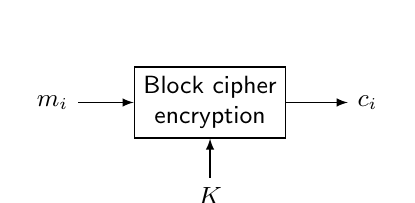
\begin{tikzpicture}[scale=1, every node/.style={scale=1}, node distance=2cm, font=\small\sffamily]
		\node[draw,align=center]     (encryption)  {Block cipher\\encryption};
		\node[left of=encryption]  (plaintext)   {$m_i$};
		\node[right of=encryption] (ciphertext)  {$c_i$};
		\node[below=0.5cm of encryption] (key-e) {$K$};
		
		\draw[->] (plaintext.east) -- (encryption.west);
		\draw[->] (encryption.east) -- (ciphertext.west);
		\draw[->] (key-e.north) -- (encryption.south);
	\end{tikzpicture}
	\caption{Encryption of a plaintext block with a block cipher}
	\label{fig:kappa-blockcipher}
\end{figure}
The differences from the general description of a cipher from Figure~\ref{fig:kappa-encdec} earlier are that the key is symmetric, and thus denoted simply by $K$, and that the plaintext and ciphertext are divided into \emph{blocks} of fixed size.
One block of the message $m$ is denoted $m_i$, and the same is true for the ciphertext blocks $c_i$.
A block cipher is a permutation from the plaintext space to the ciphertext space, but the permutation depends on the key $K$, such that knowledge of $K$ is required to map a block $m_i$ to $c_i$, and vice versa.
Worth noting is that to use a block cipher, it must be combined with a \emph{mode of operation}, which uses the block cipher as a building block.
For an in depth discussion about block ciphers and modes of operation refer to \cite{smart:2016}.
Instead, we now move on to stream ciphers.

\subsection{Stream Ciphers} \label{sec:kappa-streamciphers}

A stream cipher is a symmetric cipher that works on a stream of symbols.
The cipher generates a keystream, commonly denoted by $z$, which is used both to encrypt a message, and to decrypt a corresponding ciphertext.
The keystream is a pseudo-random stream of symbols generated by providing a key $K$ and public initialization vector $IV$ to the cipher.

Encryption is performed by combining the keystream with the plaintext using an output function $h$ as
\begin{equation} \label{eq:kappa-streamcipherencrypt}
	c_i = h(m_i, z_i) \,,
\end{equation}
where $c_i$, $m_i$, and $z_i$ are the $i^{\text{th}}$ symbol of the ciphertext, message, and keystream, respectively.
In a similar way, decryption is performed by
\begin{equation} \label{eq:kappa-streamcipherdecrypt}
	m_i = h^{-1}(c_i, z_i) \,.
\end{equation}

There are two main categories of stream ciphers, which differ in the way the keystream $z$ is constructed: \emph{synchronous} and \emph{self-synchronizing} stream ciphers.
The main difference is that synchronous stream ciphers generate keystream using only key and IV, while in self-synchronizing stream ciphers, the keystream also depends on previous ciphertext symbols.
The most common type is the synchronous stream cipher, which will be described in more detail below.

The general design of a synchronous stream cipher can be seen in Figure~\ref{fig:kappa-syncstreamcipher}.
\begin{figure}[ht]
	\centering
	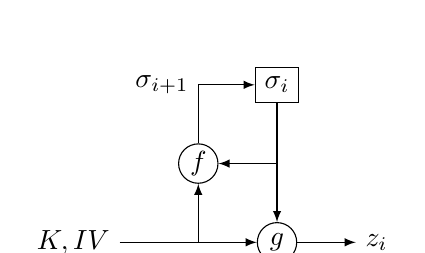
\begin{tikzpicture}[scale=1, every node/.style={scale=1}, node distance=1cm]
		\node[draw,circle,align=left,inner sep=0pt,minimum size=0.5cm]     (g)  {$g$};
		\node[right of=g,anchor=west] (z) {$z_i$};
		\coordinate[left of=g]  (kgmiddle);
		\node[left of=kgmiddle,anchor=east] (k)    {$K, IV$};
		\coordinate[above of=g] (sigmagmiddle);
		\node[draw,circle,inner sep=0pt,minimum size=0.5cm] (f) at (kgmiddle |- sigmagmiddle) {$f$};
		\node[draw,above of=sigmagmiddle] (sigma) {$\sigma_i$};
				
		\draw[->] (k) -- (kgmiddle) -- (f);
		\draw[->] (kgmiddle) -- (g);
		
		\draw[->] (sigma) -- (sigmagmiddle) -- (g);
		\draw[->] (sigmagmiddle) -- (f);
		
		\draw[->] (f) |- node[left] {$\sigma_{i+1}$} (sigma);
		
		\draw[->] (g) -- (z);
	\end{tikzpicture}
	\caption{A general figure of a synchronous stream cipher, taking key and IV as input, and outputting keystream}
	\label{fig:kappa-syncstreamcipher}
\end{figure}
The cipher has an internal state $\sigma$ which for every symbol $i$ is updated to the next state $\sigma_{i+1}$ by the next-state function $f$, which can depend on the key, IV, and current state $\sigma_i$.
For every symbol, the function $g$ calculates the current keystream symbol $z_i$, which depends on the current state $\sigma_i$, the key, and the IV.
Finally, as in (\ref{eq:kappa-streamcipherencrypt}) and (\ref{eq:kappa-streamcipherdecrypt}), the keystream is combined with the plaintext or ciphertext to perform encryption or decryption, respectively.
Stream ciphers generally also have an \emph{initialization phase}, performed before the ciphers start to generate actual keystream.
The initialization phase is not shown in Figure~\ref{fig:kappa-syncstreamcipher}, but will be discussed in more detail later in Section~\ref{sec:kappa-streamcipherinitialization}.

The most common design of synchronous stream ciphers is the \emph{binary additive stream cipher}.
This design has the following properties:
\begin{itemize}
	\item Each plaintext, ciphertext, and keystream symbol is a binary digit.
	\item The output function $h$ is the logical exclusive or operation (XOR), hereafter denoted $\oplus$.
\end{itemize}
Thus, encryption of a plaintext bit $m_i$ and decryption of a ciphertext bit $c_i$ is made with the output functions
\begin{align}
	h(m_i, z_i) &= m_i \oplus z_i        \label{eq:kappa-additiveencrypt} \\
	h^{-1}(c_i, z_i) &= c_i \oplus z_i   \label{eq:kappa-additivedecrypt}
\end{align}
using the keystream bit $z_i$.
We can easily show that this works since

\begin{equation}
	h^{-1}( h(m_i, z_i), z_i) = m_i \oplus z_i \oplus z_i = m_i \,.
\end{equation}
It is worth noting that this is a design where encryption and decryption are done in the same way -- avoiding the need for separate implementations of encryption and decryption, which is the case for some block cipher modes of operation, e.g., CBC mode.

The binary additive stream cipher above mimics another well-known cryptosystem called the \emph{one-time pad}.
In a one-time pad, each keystream symbol $z_i$ is independently and randomly generated, and then added to the plaintext just as in (\ref{eq:kappa-additiveencrypt}).
Furthermore, such a keystream must only be used \emph{once} -- giving the cryptosystem its name -- which also implies that the keystream much be at least as long as the plaintext.
While such a system may be inconvenient due to the large keystream that needs to be distributed, it has an extremely strong security guarantee, it is \emph{unconditionally secure}.
Next, we describe this and several other definitions of security.

\subsection{Security}

What does it mean for a cipher to be secure?
Indeed, there are several different definitions of what security means in this context.
While the terminology may differ slightly in the field of cryptography, these are the definitions used throughout this dissertation.

\subsubsection{Unconditional Security}

Unconditional security, or information-theoretic security, means that an adversary cannot break the cryptosystem, even with unlimited computing power.
As described earlier, the one-time pad is an example of such a system.

\subsubsection{Provable Security}

In some cases, it may be possible to base a cryptosystem on a problem that is thought to be hard.
If it is possible to prove that breaking the cryptosystem is related to solving some other well-known hard problem, the cryptosystem is said to by provably secure.
This is especially common in asymmetric cryptography, where many cryptosystems are designed to be related to well-known mathematical problems that are hard to solve.

An example of such a system with a corresponding problem is RSA \cite{rivest:1978}, which is based on the RSA problem, which can be stated as: Given a ciphertext $c$, and $e$ such that $\gcd(e, \phi(N)) = 1$, find the plaintext $m$ such that $m^e = c \mod N$.

\subsubsection{Empirical Security}
A weaker assumption is that of empirical security.
A cipher is empirically secure if empirical methods have been used to design and analyse it.
The rationale behind calling it secure is this: if a cipher has been thoroughly analysed during some longer time frame, without any attacks being found, it can be seen as secure.
While the approach is pragmatic, there are no formal proofs for security, and a new attack may be found in the future.

\subsection{Attacks}

Given that the whole purpose of a cipher is to conceal valuable information from an adversary, it is only natural that ciphers are under attack from both adversaries, as well as those wanting to select a cipher to protect their own information.
Attacks come in many forms, and can be categorized depending on their properties.
In this section, a few different kind of attacks and attack models will be described, with focus on those that are relevant for this dissertation.

\subsubsection{Key-recovery Attacks}

The goal of a key-recovery attack is simple: to gain access to the secret key $K$.
Knowledge of the key allows an adversary to decrypt ciphertexts.

\subsubsection{State-recovery}

In a state-recovery attack, the goal is to recover the internal state of the cipher.
In the case of a stream cipher, knowing the internal state at time $t$ may allow an attacker to construct a valid keystream from time $t$ and forward, which can be used to decrypt ciphertexts.
Depending on the cipher, it may also be possible to calculate earlier keystream bits, if the next-state function $f$ is invertible.
In addition, if both the next-state function $f$ \emph{and} the initialization phase is invertible, the key can be recovered, thus turning into a key-recovery attack.

\subsubsection{Distinguishers}

In a distinguishing attack, the goal for the attacker is to determine if a sequence of symbols comes from a stream cipher, or is just random data.
Consider the scenario in Figure~\ref{fig:kappa-distinguisher}.
\begin{figure}[ht]
	\centering
	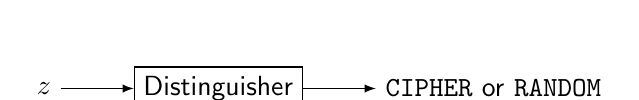
\begin{tikzpicture}[scale=1, every node/.style={scale=1}, node distance=2cm, font=\sffamily]
		\node[draw]     (distinguisher)  {Distinguisher};
		\node[left of=distinguisher,anchor=east] (keystream) {$z$};
		\node[right of=distinguisher,anchor=west] (result) {\texttt{CIPHER} or \texttt{RANDOM}};
		
		\draw[->] (keystream) -- (distinguisher);
		\draw[->] (distinguisher) -- (result);
	\end{tikzpicture}
	\caption{A distinguisher taking keystream $z$ as input, and outputting a decision}
	\label{fig:kappa-distinguisher}
\end{figure}
The goal of the distinguisher is to determine if the given keystream $z$ is produced by a cipher, or if it is just random data.
Naturally, for a given keystream, the distinguisher can always guess the correct answer with a probability of 0.5, simply by picking \texttt{RANDOM} or \texttt{CIPHER} uniformly random.
Thus a distinguishing attack is only considered successful if the distinguisher can guess the result with a higher probability compared to a uniformly random guess.
While the attack is not as strong as for example a key-recovery attack, it is still useful in a number of settings.
First, it may be possible to use the distinguisher as a part of a key-recovery attack, as done in \cite{englund:2005} and \cite{hell:2007}.
Second, if an adversary knows that a ciphertext is the encryption of one of two possible plaintexts, their respective keystreams can be derived, and passed through the distinguisher to determine which of the two plaintexts that were likely sent.
Third, the distinguisher is a useful tool in the design of stream ciphers, since the keystream from a well-designed cipher should appear random to an outside observer without the key.
This third and final use case is discussed in more detail next.

\subsection{Stream Cipher Initialization and Design}
\label{sec:kappa-streamcipherinitialization}

In Section~\ref{sec:kappa-streamciphers}, an overview of synchronous stream ciphers is given, describing the internals of the cipher and how keystream is generated.
Recall that the IV is public, and easily accessible to an attacker, thus it is important that knowledge of the IV does not allow an attacker to gain information about the keystream.
To prevent this, ciphers can mix IV and key bits during an \emph{initialization phase}, before the cipher starts to output actual keystream symbols.

One possible way to perform initialization is to repeatedly apply the next-state function $f$ \emph{before} the cipher starts to generate keystream.
Each such repeated application of the update function $f$ is called a \emph{round}.
This approach is shown in Figure~\ref{fig:kappa-cipherinitialization}.
\begin{figure}[ht]
	\centering
	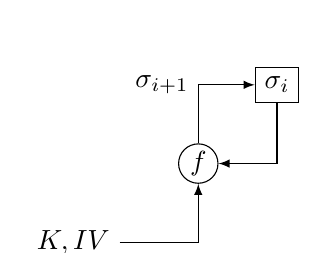
\begin{tikzpicture}[scale=1, every node/.style={scale=1}, node distance=1cm]
	\node[circle,align=left,inner sep=0pt,minimum size=0.5cm]     (g)  {};
	\coordinate[left of=g]  (kgmiddle);
	\node[left of=kgmiddle,anchor=east] (k)    {$K, IV$};
	\coordinate[above of=g] (sigmagmiddle);
	\node[draw,circle,inner sep=0pt,minimum size=0.5cm] (f) at (kgmiddle |- sigmagmiddle) {$f$};
	\node[draw,above of=sigmagmiddle] (sigma) {$\sigma_i$};
	
	\draw[->] (k) -- (kgmiddle) -- (f);
	\draw[->] (sigma) |- (f);
	
	\draw[->] (f) |- node[left] {$\sigma_{i+1}$} (sigma);
	\end{tikzpicture}
	\caption{One way to perform the initialization phase by repeatedly applying the next-state function $f$ to update the state $\sigma_i$}
	\label{fig:kappa-cipherinitialization}
\end{figure}
The initialization phase typically consist of a number of such initialization rounds, and an important part of designing the cipher is to select a suitable amount of rounds.
If too many rounds are performed, the performance of the cipher will suffer, since there is an increased delay before the cipher can start to output actual keystream.
On the other hand, if too few rounds are used, it may be possible to attack the cipher since the mixing of key and IV bits is insufficient.

To try to find such insufficient mixing, a chosen-IV attack can be performed.
As the name implies, in this setting the attacker can freely modify the IV of the cipher.
One way to perform such an attack is to look at certain keystream bits, and analyse the algebraic structure of such a bit.
One such attack was performed in \cite{saarinen:2006}, in which Saarinen used the $d$-Monomial test introduced by \cite{filiol:2002} to analyse the algebraic normal form (ANF) of certain keystream bits.

A Boolean function of $b$ variables, $f \colon \mathbb{F}_2^b \to \mathbb{F}_2$, can be written on ANF, which has the following structure:
\begin{align*}
	f(x_1, \ldots, x_b) = c_0 \oplus c_1 x_1 \oplus \ldots \oplus c_b x_b \oplus c_{b+1} x_1 x_2 \oplus \ldots \oplus c_m x_1 x_2 \ldots x_b \,,
\end{align*}
where the coefficients $c_i \in \mathbb{F}_2$ describe if the term is included in the ANF or not.
The ANF consists of up to $2^b$ monomials, with an average of $2^{b-1}$ monomials in a random Boolean function $f$.
Furthermore, if $k$ is the degree of such a monomial ($0 \le k \le b$), the ANF has on average $\frac{1}{2} {\binom{b}{k}}$ monomials of degree $k$.
The reader is referred to \cite{filiol:2002} for proofs.

The previously mentioned average monomial count can be used to perform statistical tests.
In \cite{saarinen:2006}, the $\chi^2$ test is used to analyse if the Boolean functions of the ciphers' keystream bits are biased, for monomials up to degree $d=4$.

A similar approach was presented in \cite{englund:2007}, where the $d$-Monomial test is replaced with a Maximum Degree Monomial (MDM) test, where only the monomial of the highest degree is considered, i.e., $d=b$.
The rationale behind this approach is that the maximum degree monomial is only likely to exist in the ANF if there has been sufficient mixing of the IV bits.
Furthermore, finding the coefficient $c_m$ of the maximum degree monomial can be done simply by calculating $c_m$ as:
\begin{align}
	c_m = \bigoplus_{\bm{x} \in \mathbb{F}^b_2}^{} f(\bm{x}) \,.
\end{align}

In this context, it is also relevant to mention AIDA and Cube Attacks, introduced in \cite{vielhaber:2007} and \cite{dinur:2009}, respectively.
These attacks are key-recovery attacks, thus trying to derive the secret key of the cipher.
In both papers modified versions of the cipher Trivium \cite{canniere:2006} are attacked, where the modifications consist of reducing the number of initialization rounds.

A property shared between \cite{saarinen:2006,englund:2007,vielhaber:2007,dinur:2009} is that they work on a \emph{subset} of IV bits.
The selection of this subset is a problem in itself, since it affects the outcome of the attack.
In \cite{stankovski:2010}, \citeauthor{stankovski:2010} considers this problem and presents a greedy, iterative, algorithm to find subsets of increasingly large sizes.
In addition, subsets of both IV and key bits are considered.
The author also defines the \emph{MDM signature}, which is used as a metric in the greedy algorithm.
The MDM signature is based on the MDM test described above; recall that the coefficient of the maximum degree monomial can be found by summing over all entries in the truth table.
In the MDM signature this is extended, so instead of looking at a single coefficient from the cipher's first keystream bit, the output from the (normally suppressed) initialization phase is considered instead.
Thus, if a cipher has $l$ initialization rounds, the MDM signature will consist of $l$ coefficients, each one corresponding to the coefficient of the maximum degree monomial of that particular output bit, giving a signature on the following form:
\begin{align}
	\underbrace{0000000111010110\ldots101}_{l\text{ coefficients}} \,.
\end{align}

The idea of this metric is that the lack of ones in the beginning of the MDM signature corresponds to an insufficient mixing of IV bits in the cipher, since the  maximum degree monomial has not yet been seen.

However, since finding the MDM coefficients requires summing over all entries in the truth table, it is infeasible to consider all Boolean input bits, since this would correspond to $2^b$ invocations, where $b=128$ or even more for modern ciphers.
Instead, the author tries to maximize the number of initial zeros in the MDM signature, and greedily adds more IV bits to the subset to maximize this metric.

In \paperref{ch:slightlygreedy}, we consider precisely this problem of finding subsets for attacks such as those described earlier.
While \cite{stankovski:2010} selected the subsets in a greedy fashion, we propose a generalized version, finding better subsets.
The main observation is that greedy algorithms risk getting stuck in local optima, which our generalized algorithm avoids by keeping a list of several good candidates from previous iterations.
Furthermore, the algorithm can add more than one bit in each iteration, at the expense of higher computational complexity.

Further work in the area has been done in \cite{yang:2019}, where a new algorithm is proposed, building upon the work in \paperref{ch:slightlygreedy}.
Instead of requiring the summation of all possible IV combinations (thus having a complexity of $\mathcal{O}(2^n)$ for a subset of size $n$), the authors use an algorithm to estimate the degree of the monomial instead.
This allows them to find larger subsets with lower computational complexity.

\chapter{Contributions and Conclusions}

This dissertation has focused on different preventive measures in the area of cyber security.
The different contributions can be visualized within the area as in Figure~\ref{fig:kappa-contributions}, where only preventive measures that have been covered in this dissertation are included.
After this, the contributions are described in more detail in Section~\ref{sec:kappa-contributions}, followed by conclusions in Section~\ref{sec:kappa-conclusions}.

\begin{figure}[ht]
	\centering
	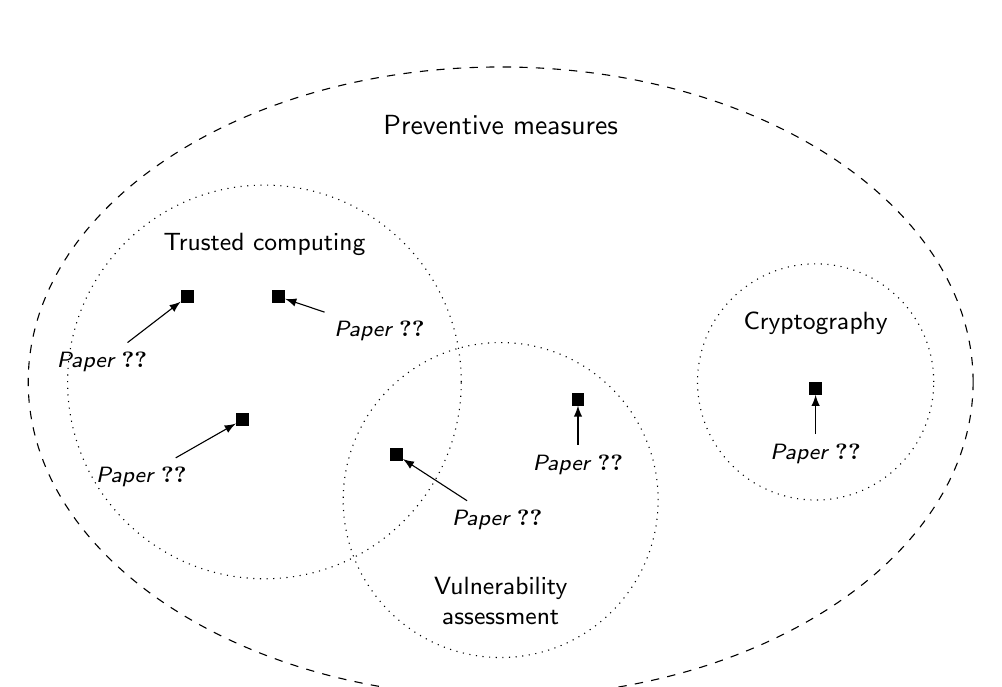
\begin{tikzpicture}[scale=1.0, every node/.style={scale=1.0,font=\sffamily}, node distance=2cm,
			area/.style={draw,dotted,ellipse,font=\small\sffamily},
			label/.style={align=center,font=\small\sffamily},
			paper/.style={draw,fill=black,minimum width=0.15cm,minimum height=0.15cm,inner sep=0pt},
			paperlabel/.style={font=\footnotesize\sffamily\itshape}]
		
		\node[draw,dashed,ellipse,minimum width=12cm,minimum height=8cm] (preventive) at (0,0) {};
		\node[below=0.5cm of preventive.north] {Preventive measures};
		
		\node[area,minimum width=5cm,minimum height=5cm,anchor=west,right=0.5cm of preventive.west] (tc) {};
		\node[label,below=0.5cm of tc.north] {Trusted computing};
		
		\node[area,minimum width=3cm,minimum height=3cm,anchor=east,left=0.5cm of preventive.east] (crypto) {};
		\node[label,below=0.5cm of crypto.north] {Cryptography};
		
		\node[area,minimum width=4cm,minimum height=4cm,anchor=east,above=0.5cm of preventive.south] (vuln) {};
		\node[label,above=0.3cm of vuln.south] {Vulnerability\\assessment};
		
		% The paper coordinates
		
		\node[paper,above left=1.0cm and 0.9cm of tc.center] (paperI) {};
		\node[paper,above right=1.0cm and 0.1cm of tc.center] (paperII) {};
		\node[paper,below left=0.4cm and 0.2cm of tc.center] (paperIII) {};
		\node[paper,above right=1.2cm and 0.9cm of vuln.center] (paperIV) {};
		\node[paper] (paperV) at ($(vuln.north west)!0.5!(tc.south east)$) {};
		\node[paper,below=0.0cm of crypto.center] (paperVI) {};
		
		% Paper labels and arrows
		\node[paperlabel,below left=0.5cm and 0.3cm of paperI] (paperIlabel) {\paperref{ch:tpmhas}};
		\node[paperlabel,below right=0.1cm and 0.5cm of paperII] (paperIIlabel) {\paperref{ch:tpm12to20}};
		\node[paperlabel,below left=0.4cm and 0.5cm of paperIII] (paperIIIlabel) {\paperref{ch:trustanchors}};
		\node[paperlabel,below right=0.5cm and 0.5cm of paperV] (paperVlabel) {\paperref{ch:recsyssgx}};
		\node[paperlabel,below=0.5cm of paperIV] (paperIVlabel) {\paperref{ch:recsys}};
		\node[paperlabel,below=0.5cm of paperVI] (paperVIlabel) {\paperref{ch:slightlygreedy}};
		
		\draw[->] (paperIlabel)   -- (paperI);
		\draw[->] (paperIIlabel)  -- (paperII);
		\draw[->] (paperIIIlabel) -- (paperIII);
		\draw[->] (paperIVlabel)  -- (paperIV);
		\draw[->] (paperVlabel)   -- (paperV);
		\draw[->] (paperVIlabel)  -- (paperVI);
	\end{tikzpicture}
	\caption{The different contributions of this dissertation to the area of preventive measures in cyber security. Each paper is positioned according to the area (or areas) it contributes to.}
	\label{fig:kappa-contributions}
\end{figure}


\section{Contributions}
\label{sec:kappa-contributions}

In this section the main contributions of this dissertation are described.
To give a quick overview, the contributions are:

\begin{itemize}
  \item A way of using TPM secure storage in high availability systems (\paperref{ch:tpmhas}), where we describe a use case where the TPM is used to store key material in a high availability system, consisting of multiple independent Computational Units (CUs) for availability purposes.
  The secure storage must be duplicated on each individual CU for availability purposes, and we describe a solution for this, supporting both TPM 1.2 and TPM 2.0.

  \item The migration of keys from TPM 1.2 to TPM 2.0, while still retaining behaviour with regard to, e.g., authorization, PCR values, and migration, even though the TPM 2.0 standard is not backwards-compatible by design (\paperref{ch:tpm12to20}).
  The proposed design utilizes new features of TPM 2.0 to achieve the behaviour of TPM 1.2.

  \item A design to protect core assets and enrollment of network security elements used in Softward Defined Networking (SDN) entities (\paperref{ch:trustanchors}).
  We describe both a way to protect core assets such as credentials by using isolated execution environments, and also a mechanism to perform secure enrollment of entities into the SDN by using remote attestation.

  \item A recommender system that generates user-specific scorings for software vulnerabilities (\paperref{ch:recsys}).
  The system takes explicit user preferences into account, together with information learned from previous interactions with the system, and creates a user profile.
  The profile is then used to generate a vulnerability scoring that is customized to the user, as opposed to other severity metrics such as the CVSS score.

  \item A privacy-preserving mechanism that can be used to protect the client profile in recommender systems for software vulnerabilities (\paperref{ch:recsyssgx}).
  Such profiles contain information about how clients have interacted with previous software vulnerabilities, as well as client preferences about vulnerability properties, which may be undesirable to share with the service provider.
  The proposed solution protects the privacy of the data such that the service provider cannot infer the real profile of a particular client.

  \item Finally, in the field of cryptography, an algorithm to find subsets for the Maximum Degree Monomial test (\paperref{ch:slightlygreedy}).
  The algorithm is easily tuned to the desired computational complexity, and produces better results compared to previous greedy approaches.
  
\end{itemize}
The following sections describe each contribution in more detail.

\subsection{\paperItitle}

In \paperref{ch:tpmhas} we describe how to use TPM secure storage in a High Availability System (HAS).
A HAS consists of multiple, redundant, Computational Units (CUs), where each CU should be able to use the secure storage.
In such systems, malfunctioning computational units can be removed and replaced with new units without downtime.
This requires the secure storage to be duplicated on each individual CU for availability purposes.

We consider a scenario with four major actors: a CU manufacturer, a HAS manufacturer, customers, and a Trusted Third Party (TTP) during migrations.
In the scenario, we consider a threat model where customer employees can copy data from drives in the HAS cabinet, that complete CU boards can be stolen, and that employees of the HAS manufacturer can access HAS data during assembly.
Apart from the threat model, the paper also specifies several other requirements that the solution should fulfil.
The overall goal is to protect stolen encrypted data from being accessed in decrypted form, while still maintaining availability guarantees using multiple redundant CUs.

The proposed solution creates a parent key, which is identical for all CUs produced by a manufacturer.
By making this key a CMK in TPM 1.2, or by using policies in TPM 2.0, migration of the key can be restricted such that only the TTP can migrate the parent key to a new TPM.
Assuming the TTP can be trusted, this guarantees that the parent key can not be migrated outside a TPM.
After this, a customer-specific key is generated, in one of three possible ways, and placed as a child to the parent key.
This key is not explicitly migratable, which means that even a malicious employee of the customer cannot migrate the key.
The key can, however, be loaded into any CU produced by the CU manufacturer, since all units share the same parent key.

A security analysis is then performed, showing that the proposed solution fulfills all the requirements, and suits the threat model as described in the beginning of the paper.
The analysis continues by comparing the three different ways to generate the customer-specific key, and describes how the different options affect the security.

To prove the feasibility of the solution, the paper also describes in detail the TPM commands that need to be used in each step of the solution, including parent key generation, customer-specific key generation, and CU replacement.
Commands are provided for both TPM 1.2 and TPM 2.0.
To further show that the solution works, the solution was also implemented using TPM emulators for both TPM 1.2 and TPM 2.0.

\subsection{\paperIItitle}

In \paperref{ch:tpm12to20} we provide an upgrade path from TPM 1.2 to TPM 2.0 by designing a solution that migrates keys from TPM 1.2 to TPM 2.0, and still retains the original behaviour of the key with regard to authorization.
Because of the differences and lack of backwards compatibility between the two TPM versions, this is a non-trivial task, but it can be achieved with careful use of the flexible policies in TPM 2.0 to simulate the behaviour of the TPM 1.2 standard.

We start by defining a set of requirements, such as keeping the same key material, keeping authorization requirements, and supporting all key types.
The requirements essentially guarantees that the behaviour with regard to key usage should be identical on the source and destination despite the different TPM versions.

The paper then describes the proposed solution from the viewpoint of four different migration scenarios:
\begin{enumerate}
	\item Migration of a single, simple, decryption or signing key.
	\item Migration of a key requiring a certain state of the PCRs.
	\item Migration of storage key, including child keys.
	\item The scenarios above, but for CMKs.
\end{enumerate}
Together these scenarios cover the different migratable key types.

The conversion is done by introducing a trusted \emph{conversion authority} which performs the conversion of the keys.
An important property of the proposed solution is that the introduction of this conversion authority does not lower the security of the system.
If the original key is a CMK, there is already a TTP in control of migration (the MSA), which could potentially be extended to also support conversion.
If the original key is not a CMK, the owner can already freely migrate the key to any destination.
Thus, the owner can perform the operations of the conversion authority locally at the source or destination TPM, if a separate conversion authority is undesirable.

Finally, the paper also describes the implementation process to test the proposed migration scenarios.
The conversion authority was implemented and tested by using TPM emulators for TPM 1.2 and TPM 2.0.

\subsection{\paperIIItitle}

In \paperref{ch:trustanchors} we contribute to the area of security in Software Defined Networking.
The contributions from this paper can be divided into two major parts: first we protect security assets of network elements using isolated execution environments with a new library called TLSonSGX, and second a mechanism for secure enrollment of network elements in software defined networks.
Both parts use trusted computing to achieve their respective goals, both TPM and Intel SGX.
The two parts are described in more detail below.

\subsubsection{TLSonSGX}

The data plane in an SDN deployment consists of for example virtual switches that are deployed by an orchestrator.
The virtual switches are dynamically connected to virtual instances as they are created and destroyed.
Communication between the data plane and the central SDN controller happens over the southbound API, ideally using TLS with mutual authentication to protect the SDN deployment.

TLSonSGX allows virtual switches to use a cryptographic library that runs inside a TEE.
By providing a wrapper around the OpenSSL API, but with selected functions leading into an SGX enclave, the library can ensure that TLS sessions originate and terminate within the enclave.
Thus, certificates used for mutual TLS authentication can be stored securely within the enclave, protecting the confidentiality and integrity of such security assets even in case of a compromise of the host.
By providing the library as a wrapper around a subset of the OpenSSL API, we could use the library together with Open~vSwitch.

Finally, TLSonSGX was evaluated by measuring several aspects including generation time of keys and certificates, and packet round trip latency.
While key generation is only performed upon launch of Open vSwitch, the packet round trip latency affects all packages in the TLS connection.
The evaluation shows that the latency is increased compared to using OpenSSL outside the enclave, since there is an overhead when entering and exiting the enclave for packets.
However, based on the system model of a typical SDN deployment, only the first packet of flow will be passed to the controller, after this the switch will have learned the flow and the latency between controller and virtual switch is irrelevant.

\subsubsection{Secure Enrollment of Network Elements}

Before enrolling network elements such as VNFs in the network infrastructure, their integrity should be verified, since only trustworthy applications should be able to communicate with the SDN controller.
The paper proposes a solution where the integrity of a VNF is verified by using the TPM as a root of trust.
In addition, SGX enclaves are used to ensure integrity and confidentiality of credentials required for communication with the SDN controller.
This provides an extra layer of protection in case of a breach of the platform TCB.

In the proposed solution, the VNF requires credentials in form of a client certificate to be able to connect and communicate with the SDN controller.
To acquire valid credentials, the VNF must first pass integrity checks.
Integrity measurements are provided by Linux IMA, which can also use a TPM to anchor the measurements.
The TPM can be used for remote attestation, and a certificate authority can compare the signed quote of the platform state with a list of known good configurations.
If the quote is known to be good, the CA issues a signed client certificate back to the VNF which can then use it to connect to the SDN controller.
The signed client certificate is stored securely in an enclave.
A malicious VNF would not be able to acquire such a certificate, and will not be enrolled.

The enrollment scheme is also implemented and evaluated in terms of performance, mainly with regard to time for enrollment, since every time a VNF is launched a new attestation sequence must be performed before enrollment.
Measurements show that the complete attestation sequence can be performed in significantly less than one second.

\subsection{\paperIVtitle}

\paperref{ch:recsys} contributes to the area of software vulnerability assessment.
The paper presents a recommender system that consists of three main subsystems: a knowledge-based, a content-based, and a domain-based.
Together, the three subsystems can deliver recommendations based on a user's explicit preferences, as well as automatically learn from the user's previous interactions with the recommender.
The domain-based subsystem is specific for the field of vulnerabilities, and allows the provider of the recommender to configure rules that are specifically adapted to the field of vulnerabilities.

The proposed recommender is implemented with a set of different vulnerability features as data sources for the recommender.
Suggested features includes both common vulnerability metrics such as confidentiality, integrity, and availability impact from CVSS, but also includes other sources such as the availability of Metasploit exploits, and Google hits.

While the standard CVSS score is the same for all users, the CVSS specification also allows for the use of an \emph{environmental} score \cite{cvss2spec,cvss3spec}.
This allows users to manually select the importance of a set of properties which affect the final weights of the score.
Comparing our proposed recommender to the CVSS environmental score is a relevant comparison to make, since they both allow for user-specific vulnerability scoring.

An initial evaluation of the proposed recommender is provided in the paper, where an offline data set is collected from a set of users working in the industry, for different companies, and with high security awareness -- potential users of such a recommender system.
After asking the users to manually rank a set of CVEs, and state their preferences regarding aspects of vulnerabilities in general, we could evaluate the effectiveness of the score produced by the recommender.
The evaluation shows a higher predictive rating accuracy for most users when using the recommender compared to using the environmental score.

\subsection{\paperVtitle}

In \paperref{ch:recsyssgx} we consider the privacy implications of a recommender such as the one described in \paperref{ch:recsys}.
Stored user profiles, containing both implicit and explicit user preferences, could be used by a malicious actor to gain information about internal security policies.

The paper addresses this problem by describing a privacy-preserving mechanism to protect the user profiles.
The solution is based on both trusted execution environments together with an approach derived from $k$-anonymity and differential privacy.
The overall idea is to release queries to the recommender in larger batches, where the genuine profile is sent together with statistically different pseudo profiles, thus preventing a malicious service provider to match a user with a profile.

The paper proposes a design utilizing a TEE, allowing the privacy-preserving solution to be provided by either a third-party, or the service provider itself.
Regardless of the location, the client can verify the integrity of the intermediary to be sure that it has not been tampered in a way that could destroy the privacy guarantees.
This also allows the intermediary to be placed in near proximity of the recommender system, which may reduce network delays when multiple queries are issued.

We also describe the implementation of a prototype, implemented using Intel SGX, and tested it with an already existing recommender system.
The proposed implementation requires no modifications of the recommender system itself, which together with the possibility for a third-party intermediary allows for a gradual adoption.
Finally, the prototype implementation is evaluated in terms of performance, to show the performance impact of the proposed solution.
As expected, by introducing the extra pseudo-profiles, the response time is increased because the recommender needs to handle more requests.
This highlights the trade-off between privacy guarantees and response time of the recommender.

\subsection{\paperVItitle}

In \paperref{ch:slightlygreedy} we focus on the construction of distinguishers and nonrandomness detectors, specifically on the use of the Maximum Degree Monomial (MDM) test.
This test was introduced in \cite{englund:2007}, and requires the use of a subset of IV and/or key bits which are analysed.
The selection of such subsets was considered in \cite{stankovski:2010}, where a greedy algorithm was proposed.

Greedy algorithms risk getting stuck in local optima, which may not be close to the global optimum.
However, performing an exhaustive search over all possible subsets is infeasible, as recent symmetric ciphers have key and IV lengths of up to 256 bits.

Instead, we propose a new and generic algorithm to find such subsets.
The algorithm is easily tunable to the desired computational complexity, and works on any stream cipher.
It can be seen as a generalization of the greedy algorithm proposed in \cite{stankovski:2010}, but instead of always greedily choosing the best bit in each iteration, our algorithm keeps track of a list of good candidates in each iteration.
This reduces the risk of the algorithm to get stuck in local optima.
The algorithm also allows to add more than one bit to the subset in each iteration, which further decreases the risk of getting stuck in a local optima, at the expense of increased computational complexity.

The algorithm is evaluated by comparing several different input parameters, both to show the possibilities of the algorithm, as well as providing an idea as of how different parameters affect the final results.
The evaluation is performed on several different ciphers: Grain-128a, Kreyvium, and Grain-128, and consistently provides better results compared to the na\"{i}ve greedy approach.

The paper is an extended version of \cite{karlsson:2017}, where the analysis of Kreyvium has been added, as well as more test on all ciphers such as investigating the effect of using an optimal starting set, as well as other improvements.

\section{Conclusions}
\label{sec:kappa-conclusions}

The topic of this dissertation has been to present new results on preventive measures in the area of cyber security.
The contributions have covered several fields, including trusted computing, recommender systems, and cryptography.

The diversity of the contributions also shows that the security of a system as a whole depends on many parts; ciphers need to be secure, only expected code should execute, and the code that actually runs should be free from software vulnerabilities.
While all parts are relevant for a secure system, they may also be managed by different people, and realistically, the contributions of this dissertation are aimed at different practitioners.

Contributions presented in \paperref{ch:tpmhas}, \paperref{ch:tpm12to20}, and \paperref{ch:trustanchors}, are useful for system designers, and providers of services in a high-availability or cloud setting.
Tools such as the recommender system for vulnerabilities presented in \paperref{ch:recsys}, together with the privacy-enhancing methods from \paperref{ch:recsyssgx}, can be useful in a more direct way to a broader range of people -- they can be used directly by developers to detect vulnerabilities in their external components.
In contrast, the tools for analysing stream ciphers presented in \paperref{ch:slightlygreedy} will realistically be used by a limited set of researchers in cryptography.

However, for all contributions, users can indirectly or directly benefit from the increase in security.
It also shows that the responsibility for an overall secure system is in the hands of many people -- where each party is responsible for their individual piece.

{ \raggedright
\printbibliography[segment=\therefsegment,heading=bibintoc]
}


% Remove the LaTeX chapter from all numberings in included papers.
% theHchapter is set so that \setcounter{chapter}{0} below doesn't cause clashes.
\renewcommand{\thesection}{\arabic{section}}
\renewcommand{\thefigure}{\arabic{figure}}
\renewcommand{\thetable}{\arabic{table}}
\renewcommand{\thechapter}{\Roman{chapter}}
\renewcommand{\theHchapter}{publication.\Roman{chapter}}
\renewcommand{\theHsection}{\theHchapter.\arabic{section}}
\renewcommand{\theequation}{\arabic{equation}}

% Include a reference at the footer of each page.
\newlength{\apa}
\setlength{\apa}{0cm}
\setlength{\spiff}{0cm}

% Paper mark in margin.
\renewcommand{\markmargin}{%
\begin{tikzpicture}[remember picture, overlay]%
\node at (current page text area.north -| current page.east) [
  anchor = north east,
  yshift = -\apa,
  rectangle,
  fill = black,
  minimum width = 1.6cm,
  minimum height = 2cm,
  inner sep = 0pt,
  outer sep = 0]
  (rec) {};
\node at (rec.south west) [
  anchor = north west,
  text width = 2cm,
  text height = 0.4cm,
  inner sep = 0,
  outer sep = 0,
  text centered,
  font=\sffamily\bfseries\small,
  color=white,
  rotate=90]
  {Paper~\thechapter};
\end{tikzpicture}%
}

\newfloat{paperfoot}{b}{paper}
\newcommand{\paperRemark}[1]{
  \begin{paperfoot}%
  \hrulefill \flushleft \footnotesize #1 \end{paperfoot}
}
%-------------------------------------------------------

\part{Included Publications}

\setcounter{chapter}{0}
\renewcommand{\chaptername}{Paper}
\fancyhead[LO]{\rightmark}

\ifpaperI
\newrefsegment
\fancyhead[RE]{\paperref{ch:tpmhas}: \paperItitle}
\chapter[\paperItitle]{\texorpdfstring{%
		Using TPM Secure Storage in\\Trusted High Availability Systems}{%
		\paperItitle}}
\label{ch:tpmhas}
\paperRemark{\paperIref}

{
%\documentclass{llncs}
%\usepackage{multirow}
%\usepackage{rotating}
%\usepackage{tikz}
%\usetikzlibrary{arrows,backgrounds,positioning}
%\usepackage{enumitem}
%\usepackage{hyperref}
%\hypersetup{pdfborder=0 0 0}
%\usepackage{listings}
%\usepackage{booktabs}
%\usepackage{array}
%\usepackage{amsmath}
%\usepackage{amssymb}
%\newcolumntype{P}[1]{>{\centering\let\newline\\\arraybackslash\hspace{0pt}}m{#1}}
%\usepackage{geometry}

\makeatletter
\def\namedlabel#1#2{\begingroup
    #2%
    \def\@currentlabel{#2}%
    \phantomsection\label{#1}\endgroup    
}
\makeatother

\newenvironment{tpmcommands}{\begin{scriptsize}}{\end{scriptsize}}

\section*{Abstract}

We consider the problem of providing trusted computing functionality in high availability systems. We consider the case where data is required to be encrypted with a TPM protected key. For redundancy, and to facilitate high availability, the same TPM key is stored in multiple computational units, each one ready to take over if the main unit breaks down. This requires the TPM key to be migratable. We show how such systems can be realized using the secure storage of the TPM. Hundreds of millions TPM 1.2 chips have been shipped but with the recent introduction of TPM 2.0, more manufacturers are expected to start shipping this newer TPM. Thus, a migration from TPM 1.2 to TPM 2.0 will likely be seen in the next few years. To address this issue, we also provide an API that allows a smooth upgrade from TPM 1.2 to TPM 2.0 without having to redesign the communication protocol involving the different entities. The API has been implemented for both TPM 1.2 and TPM 2.0. 

\section{Introduction}
A High Availability System, hereafter referred to as HAS, can be used for mission critical systems like medical, trading, banking, mobile network infrastructure, and blue-light systems. Such systems often run for many years and sometimes longer than a decade.  As part of high availability requirements, often such systems need trusted platform functions that guarantee that only authentic and approved system software and applications can run on them. Also, one frequently sees demands to safely store sensitive data and keys used by applications and management functions.
%HAS and more TPMs
In the types of HAS that we consider there are multiple Computational Units (CUs) that are organized so they can take over each others' tasks in the event a CU fails. To provide for trusted platform functions like authenticated boot and storage of sensitive data and keys, each CU is equipped with a TCG Trusted Platform Module (TPM). Typically, a CU is a PCB or rack mountable unit that can be inserted in a cabinet that hosts the HAS, and can accommodate a multitude of CUs. The use of multiple TPMs for protection in a HAS has many technical problems due to the migration problems that the use of TPM introduces.
 
At the same time, there are different versions of the TPM, which in some aspects are very different from each other. TPM 1.2 was introduced in 2003 and since 2006 a TPM chip has been included in many laptops. In 2012, TPM 2.0 was introduced, adding new functionality and with no backwards compatibility with TPM 1.2. Even though PCBs still come equipped with a TPM 1.2 chip, within a few years TPM 2.0 is likely to be the dominant chip on newer boards. This provides a challenge as systems utilizing trusted computing functionality may have to undergo significant, and costly, changes.
 
In this paper, we focus on Trusted Computing Technology, and how a CU manufacturer can offer a solution where customers have unique keys, only usable in a specific HAS, but which still utilizes generic CUs to be used as replacement boards. Moreover, we provide a general API that is independent of the TPM version used. This allows for a cost-efficient deployment of the system as it can be easily updated when TPM 2.0 gains widespread adoption.

The paper is organized as follows. Section~\ref{sec:overview} gives a brief overview of TPMs, describing some functionality relevant to the paper. In Section~\ref{sec:usecase}, we specify the use cases together with the threat model. In Section~\ref{sec:requirements} we describe the requirements that must be met by the proposed solution, which is then described in Section~\ref{sec:sol}. A security analysis of the proposed solution is described in Section~\ref{sec:secanalysis}. Section~\ref{sec:unifiedapi} describes the general API. Finally we discuss some related work in Section~\ref{sec:tpmhas:relatedwork}. Section~\ref{sec:conc} concludes the paper.
 
\section{Overview of TPM 1.2 and TPM 2.0}
\label{sec:overview}
TPMs have been around for more than a decade and most laptops ship with a TPM. Still, we have seen very few applications taking advantage of the functionality provided by TPMs. Microsoft's Bitlocker encryption system is the most known and widely used. A TPM enables trusted computing functionality such as authenticated boot, remote attestation and sealed storage. This section will give a short introduction to TPM 1.2 and 2.0, highlighting the differences when duplicating keys to new destinations. For a more detailed treatment we refer to the specifications~\cite{TPM1.2spec,TPM2.0r07}.
 
\subsection{Overview of TPM 1.2 and Certifiable Migration Keys}
A TPM 1.2 provides a key hierarchy of asymmetric keys, where the private part of a child key is protected (encrypted) using the public key of the parent. Parents are of type \textit{storage key} and are used to encrypt other keys, while leafs in the tree can be of any type, e.g., a signing key, encryption key or attestation identity key (AIK). Asymmetric keys in TPM 1.2 consist of two parts: one public part, and one private part. The public part contains data such as the public key and different flags. The private part is encrypted, and contains the private key, but also usage and migration secrets. The root of the key hierarchy is the Storage Root Key (SRK), which is created when someone takes ownership of the TPM. The TPM owner authenticates using an \textit{owner secret} and several commands require owner authorization, e.g., commands used in migration which is the main topic of this paper. Commands that use the private part of a key are authenticated using a \textit{usage secret} which can be unique to each key. Such commands are e.g., creation of new keys, data signing and data decryption.
 
The only way to have the same key protected by two TPMs is to use migratable keys. Migratable keys were introduced in TPM 1.1, offering the ability to migrate (or actually duplicate) a TPM protected key to another TPM. There are two variants of migration schemes specified, called \textit{rewrap} and \textit{migrate}. In the rewrap case, the private part of the migratable key is simply decrypted and re-encrypted using the destination key. In the migrate scheme, the key is instead re-encrypted using the public key of a migration authority (MA). The MA can then re-encrypt the private part with the destination public key. We will not consider the scheme using a migration authority any further in this paper.

Each key also has a \textit{migration secret} in addition to the usage secret. Migration is only allowed if the migration secret is known. For non-migratable keys, the migration secret is \textit{tpmproof}, a value internal to the TPM and never exposed. Also, the source TPM-owner must approve the destination, however, for any migratable key, the owner can choose any destination. Thus, if the TPM owner is not trusted, the key can end up in any TPM, or even outside a TPM if the owner migrates the key to his own keypair generated by e.g., OpenSSL.

A Certifiable Migration Key (CMK), introduced in TPM 1.2, allows for a trusted entity, called Migration Selection Authority (MSA), to be in control of destinations for each individual CMK. The MSA control is tied to each CMK by binding the CMK key to a list of MSAs at key creation time (called \textit{MSAList}). Similar to migratable keys, there are two possible migration schemes for CMKs, \textit{restrict\_migrate} and \textit{restrict\_approve}. In restrict\_approve, tickets which include both the CMK and the destination public key, are used to control the destination. Tickets are signed by the MSA and only the destination in the ticket can be used as target for migration. Then the ticket is first used to create a CMK blob encrypted with the destination SRK. Then the ticket is used again in the target TPM to convert the blob into a key in the key hierarchy. The tickets signed by the MSA are called restrictTickets. From these tickets, sigTickets are produced by letting the TPM owner approve the information in the restrictTicket. Thus, both the MSA and the TPM owner control the migration of a CMK. In the following, restrictTickets will sometimes simply be denoted ``ticket'' since this is the ticket that will be communicated between entities.

In the restrict\_migrate scheme, the CMK is migrated directly to an MSA. No ticket is needed in this case since the key already is bound to the MSA at creation time so the MSA is trusted as destination.
 
Different from a migratable key, a CMK can be certified by an AIK. The certification states that the CMK key belongs to a TPM and that the private part of the key will never leave the TPM in unencrypted form (assuming the MSA enforces this). Certification of CMKs is not used in this paper and will not be considered further.
 
 
\subsection{Limitations of CMKs}
The TPM owner controls migratable keys in the sense that he/she can create them outside of the TPM or migrate them out from the TPM. Thus, there is no guarantee that the private key is TPM protected. While this problem is addressed by CMKs, putting an MSA in control, the CMKs have some important limitations.
\begin{itemize}
\item A software MSA can create CMK keys outside the TPM and migrate them into a TPM.
\item When the restrict\_migrate scheme is used, a software MSA can read the private CMK key.
\item Each time a CMK is migrated, both out of a TPM and into a new TPM, a signed ticket from an MSA is required. Thus, from the perspective of the two TPMs, there must be communication with a third party. If tickets are created in advance this is not required, but then the destinations must be known in advance.
\end{itemize}
 
The last limitation above significantly restricts the use of CMKs in HAS's, because the destination CU (e.g. a replacement unit) is not known in advance. It is therefore important to find secure ways to combat this problem. This is one of the main goals in our proposed design.
 
\subsection{Overview of TPM 2.0 and Duplication}
The key hierarchy in TPM 1.2 has been replaced by an object hierarchy in TPM 2.0. Objects in the hierarchy can be both symmetric and asymmetric keys, but also data blobs. The type is determined by a combination of the binary properties \textit{sign}, \textit{decrypt} and \textit{restricted}, where the last property means that the object (key) can only perform actions on data prepared by the TPM itself. This is controlled by including a specific byte sequence in these objects. Some commands can only be performed in objects with this byte sequence. Storage keys are asymmetric keys with the properties restricted and decrypt. Similar to TPM 1.2, these keys protect child keys in the hierarchy. However, the protection in TPM 2.0 is by symmetric encryption. A storage key has a unique seed in its private part, which is used to derive a symmetric encryption/decryption key. This key is derived from the seed each time a new object is created or loaded into the TPM.
 
In TPM 2.0 the term migration has been replaced by duplication, as it more accurately reflects the reality.
%A duplicated key, or migrated in TPM 1.2, is not removed from the source TPM.
Two important object attributes are used to control duplication of a key. The first, fixedTPM, controls if an object can be duplicated at all. If an object has this attribute set, the object can not be duplicated. Naturally, an object with fixedTPM set can not be below an object with fixedTPM clear in the hierarchy. The second, fixedParent, controls if an object can be explicitly duplicated (when fixedParent is clear) or if it must be implicitly duplicated (when fixedParent is set) by duplicating a parent key, which has fixedParent clear.
 
The notion of CMKs and migration schemes has been completely removed in TPM 2.0, and has been replaced by \textit{policies}. A policy is a general concept that controls the actions that can be performed on an object in the hierarchy. Policies are set upon object creation time by storing a value, called authPolicy, in the public part of an object. The authPolicy is a hash value created by running several policy commands, where each command extends the authPolicy digest. This is similar to how PCR values are built by using TPM\_Extend. The authPolicy can be based on e.g., time limitations on usage of the object, specific commands that are possible to execute with an object and specific parameters that can be used in a command. Before executing a command a policyDigest must be built in a policy session. This session also stores specific context values that are checked upon execution, e.g., the command code if a certain command must be executed or the fact that a certain authorization method should be used. The final policyDigest is compared to the object's authPolicy and if they match, the command is executed using the information in the context values. Policies can be combined using logical AND and OR.
 
The use of policies is in general optional as it is possible to authorize using HMAC, similar to authorization in TPM 1.2, or by directly providing a password. However, for duplication the use of policies is mandatory. Policy commands that are particularly interesting for key duplication are TPM2\_PolicyAuthorize and TPM2\_PolicyDuplicationSelect.
 
The TPM2\_PolicyAuthorize command allows a policy to change by letting an authority sign the new policy. This is done as follows. The TPM user generates a new policy to use for an object. This policy, and the properties it represents, are evaluated by an authority. If they are acceptable, the authority signs this policy and returns the signature. The signature is verified using TPM2\_VerifySignature which returns a ticket showing that the signature is valid. This ticket, together with the approved policy, is then used in the TPM2\_PolicyAuthorize command. Upon executing this command with a valid ticket, the policyDigest is updated by replacing it by the hash of the name of the signature key. This hash is then the new PolicyDigest. Thus, any policy that needs to change during the lifetime of an object needs to include the TPM2\_PolicyAuthorize command after all policies that are subject to change. Policies added after this command has been executed can not be changed.
 
The TPM2\_PolicyDuplicationSelect command is used to control the destination for a duplication. The command includes both the name of the object to be duplicated and the name of the destination. The policyDigest is updated using both these names. Thus, the policy ties the object to a specific destination (or several if logic OR is used). Since the destination is typically not known when an object is created, this is typically used together with TPM2\_PolicyAuthorize. This will allow an authority to verify that the destination is valid and then sign the resulting policyDigest.

\subsection{Platform Configuration Registers}
All TPMs, both of version 1.2 and 2.0, have a number of Platform Configuration Registers (PCRs). These registers store a hash value, which is built-up by repeatedly calling TPM\_Extend or TPM2\_Extend. This creates a cumulative hash, since an extend operation depends on both a new value and the previous PCR value. The PCRs are used to store measurements of the hardware configuration and software. The measured values are stored in the Stored Measurement Log (SML), outside the TPM, while the digest are secured by the TPM.

The SML can be read to ensure that the measurement values of the system are as expected, and the integrity of the SML can be verified by comparing them to the PCRs. In addition, keys in the TPM can be bound to certain PCR values, such that keys can only be used when the PCRs have the correct value, thus ensuring that keys are only used in a trusted hardware and software setting.

\section{Scenario and Threat Model}
\label{sec:usecase}
The considered use case aims at building a robust infrastructure, taking the HAS life cycle into consideration. The scenarios includes four entities.

The hardware, i.e., the computational units (CUs), are produced by a \textbf{CU manufacturer}. The CU boards will include a TPM but it will not be associated with any particular, or identified, customer or end user.

A HAS is assembled by a \textbf{HAS manufacturer}. The HAS manufacturer takes two or more CUs, due to the redundancy requirements, from the CU manufacturer and assembles the HAS, also using equipment from other sources. This additional equipment is outside the scope of this work.

\textbf{Customers} are purchasing a HAS on which they want to store sensitive data. This data can e.g., be keys or sensitive application data of applications running on the HAS. The sensitive data is stored in \textit{secure storage}, meaning that it resides on a hard disk in encrypted form, protected by a TPM. 

A \textbf{Trusted Third Party} (TTP) is used to enable the secure migration of keys between TPMs. This is the MSA in TPM 1.2 and authority in TPM 2.0. We assume that this party keeps all keys secure, possibly, but not necessarily, with a TPM. %A TTP is also used to guarantee that attestation identity keys in TPM 1.2 belong to a TPM. This is called PrivacyCA in TCG. The two TTPs are typically different entities and when we refer to TTP in this paper we mean the MSA/Authority. 

\subsection{Threat Model}
Any attacker that controls the hardware, will also be able to circumvent the protection offered by trusted computing, as the root of trust is potentially compromised. Thus, to this end it is natural to consider the CU manufacturer trusted and it can theoretically be merged with the TTP. It is also from the CU manufacturer's perspective we mainly treat the problem. Still, mounting an attack against the hardware is different from attacking the software controlling the migration on the TTP. We will therefore consider them as separate entities. % in this paper.
%TODO: Still, some attacks are easier to mount than others and a separation can be motivated if.....\textit{how to deal with this, should we merge them?? What is included in our threat model}

In practice, many service and operating personnel, hereafter collectively named company employees, will have access to the HAS during its lifetime. Not all company employees can be considered trusted, and this is the main reason to protect data using a TPM, as the decryption key will never leave the TPM unencrypted. Not trusting company employees will also help the customer to protect against other, potentially malicious, customers' personnel.

\begin{itemize}
\item[\namedlabel{TcustEmployees}{T1}.] Anyone, including customer employees, can copy data and software from drives in the HAS cabinet. They may also interact with the TPM.
\item[\namedlabel{Tstolen}{T2}.] CU boards can be stolen, both spare boards and those already mounted in a cabinet. Boards from customer A can be used in the HAS of customer B.
\item[\namedlabel{THAS}{T3}.] HAS manufacturer employees can access data in the HAS when it is being assembled, in particular data that is associated with the TPM.
\end{itemize}

The main goal is to protect stolen (encrypted) HAS data from being accessed in cleartext, while at the same time provide a system with very low downtime. 

\section{Requirements} \label{sec:requirements}
Based on the scenario and threat model, we define the following requirements.

\begin{itemize}
\item[\namedlabel{Rsecurity}{R1}.] \textbf{Data confidentiality.} Data stored on secondary memory, e.g., hard drives or memory cards, must always be encrypted. The key may never be stored (unencrypted) on secondary memory.
\item[\namedlabel{Rredund}{R2}.] \textbf{Redundancy.} The data on a HAS must at all times be accessible, even in the case of hardware failure.
\item[\namedlabel{Rscale}{R3}.] \textbf{Scalability.} After completed assembly by the HAS manufacturer, spare CUs can be ordered by the customer directly from the CU manufacturer. These are generic and not personalised for the specific customer. Thus, we assume that anyone will be able to buy a generic CU.
\item[\namedlabel{RcustLock}{R4}.] \textbf{Customer lockdown.} Only TPMs initiated by the CU factory can be used as replacement boards. This will allow the CU factory to create boards that are specific for a group of customers, still allowing customers to have unique keys.
\item[\namedlabel{Rpers}{R5}.] \textbf{TPM Compatibility.} The API used by the different entities must be compatible with both TPM 1.2 and TPM 2.0.
\item[\namedlabel{RcustControl}{R6}.] \textbf{Customer control.} The customer should be the owner of the TPM, allowing him to use it for other purposes such as remote attestation and key certification. This also allows the customer to reuse the hardware and TPMs in the event of a CU manufacturer going out of business.
\item[\namedlabel{RuserF}{R7}.] \textbf{User friendliness.} Replacing CUs in the HAS should be as easy as possible for the customer. This includes minimizing the online communication with other entities, possibly providing a completely offline solution. It also includes minimizing the HAS interaction needed by customer employees.
\end{itemize}

We return to these requirements in Section~\ref{sec:secanalysis} when evaluating the security of the proposed solution.


For the sake of simplifying our expositions we assume further that the HAS uses only two CUs. Thus, the key protecting the sensitive data must be identical in both TPMs so that the backup CU can immediately become active in case the first CU fails. Further, when a CU breaks it should be replaced by a spare CU from the CU manufacturer.

\section{Proposed System Design}
\label{sec:sol}
Due to the redundancy requirement (\ref{Rredund}), one key must be associated with several TPMs. This can only be done using duplicable (migratable in TPM 1.2) keys. We first analyze how this can be achieved in TPM 1.2. Consider the most straightforward solution of having a plain migratable key immediately below the SRK in the hierarchy. To migrate this key to a new SRK, the TPM owner can simply rewrap this key with the new SRK and import it to the new TPM.

\begin{scriptsize}
\begin{verbatim}
TPM_AuthorizeMigrationKey     //Owner authorized
TPM_CreateMigrationBlob       //On source TPM
TPM_ConvertMigrationBlob      //On destination TPM
\end{verbatim}
\end{scriptsize}
The main problem with this is that the owner can rewrap the key with any key, even one created outside the TPM. Thus, if the customer is the owner (\ref{RcustControl}) the private part of the key is not guaranteed to be protected by the TPM at all times (\ref{TcustEmployees}).

With CMK keys in TPM 1.2 and policies in TPM 2.0, the migration/duplication can be controlled by a trusted authority, even when the customer is the TPM owner. The migration of a key then proceeds as follows.

\begin{scriptsize}
\begin{verbatim}
TPM_CMK_ApproveMA              //On source TPM, owner authorized
TPM_CMK_CreateKey              //On source TPM
TPM_AuthorizeMigrationKey      //On source TPM, owner authorized
TPM_CMK_CreateTicket           //On source TPM, owner authorized
TPM_CMK_CreateBlob             //On source TPM
TPM_CMK_CreateTicket           //On destination TPM, owner authorized
TPM_CMK_ConvertMigration       //On destination TPM
\end{verbatim}
\end{scriptsize}
The \verb!TPM_CMK_ApproveMA! command lets the owner bind an MSA to the CMK. The ticket is signed by the MSA and the key can only be migrated to a destination given in the ticket. From this it is clear that the customer can not be owner at the time the key is first created since he could assign any key to be an MSA public key.

An important observation is that a TPM key, we call it $K_{e}$ ($e$ for encryption), can be used on several TPMs provided that the parent key $K_p$ is the same on all TPMs. The key blob is stored on (secondary) memory and loaded into the TPM when needed. Upon loading a key, it is decrypted by the parent key. Thus, if the parent key is $K_p$ it can be loaded into any TPM that has $K_p$ in the key hierarchy. In order to have $K_p$ in several TPM key hierarchies, it must be migratable and any key having a migratable key as parent key must also be migratable. Moreover, a CMK (which is migratable) may not have a migratable key as parent. Figure~\ref{migratableHierarchy} summarizes these restrictions.

\begin{figure}[h]
\centering
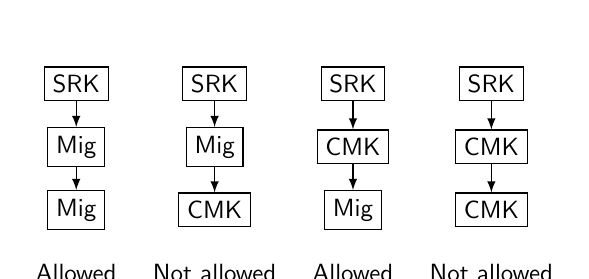
\begin{tikzpicture}[font=\sffamily]
%Case A
\begin{scope}[xshift=0]
\node[draw,align=center, scale = 0.9] (SRK) at (0,0) {SRK};
\node[draw,align=center, scale = 0.9] (mig1) at (0,-0.8) {Mig};
\node[draw,align=center, scale = 0.9] (mig2) at (0,-1.6) {Mig};
\node[align=center, scale = 0.9] (CaseA) at (0,-2.4) {Allowed};
\draw[->] (SRK.south) -- (mig1.north);
\draw[->] (mig1.south) -- (mig2.north);
\end{scope}
%Case B
\begin{scope}[xshift=50]
\node[draw,align=center, scale = 0.9] (SRK) at (0,0) {SRK};
\node[draw,align=center, scale = 0.9] (mig) at (0,-0.8) {Mig};
\node[draw,align=center, scale = 0.9] (cmk) at (0,-1.6) {CMK};
\node[align=center, scale = 0.9] (CaseA) at (0,-2.4) {Not allowed};
\draw[->] (SRK.south) -- (mig.north);
\draw[->] (mig.south) -- (cmk.north);
\end{scope}

%Case C
\begin{scope}[xshift=100]
\node[draw,align=center, scale = 0.9] (SRK) at (0,0) {SRK};
\node[draw,align=center, scale = 0.9] (cmk) at (0,-0.8) {CMK};
\node[draw,align=center, scale = 0.9] (mig) at (0,-1.6) {Mig};
\node[align=center, scale = 0.9] (CaseA) at (0,-2.4) {Allowed};
\draw[->] (SRK.south) -- (cmk.north);
\draw[->] (cmk.south) -- (mig.north);
\end{scope}

%Case D
\begin{scope}[xshift=150]
\node[draw,align=center, scale = 0.9] (SRK) at (0,0) {SRK};
\node[draw,align=center, scale = 0.9] (cmk1) at (0,-0.8) {CMK};
\node[draw,align=center, scale = 0.9] (cmk2) at (0,-1.6) {CMK};
\node[align=center, scale = 0.9] (CaseA) at (0,-2.4) {Not allowed};
\draw[->] (SRK.south) -- (cmk1.north);
\draw[->] (cmk1.south) -- (cmk2.north);
\end{scope}


\end{tikzpicture}
\caption{Key hierarchy restrictions for migratable keys. Both the \texttt{TPM\_CMK\_CreateKey} and the \texttt{TPM\_CMK\_ConvertMigration} commands verify that the parent key is not migratable.}
\label{migratableHierarchy}
\end{figure}

Thus, if we wish to be able to use $K_{e}$ in several TPMs without having to migrate it, this key must be migratable, but not a CMK. The parent key $K_p$ can be either a plain migratable key or a CMK. Since $K_p$ must be explicitly migrated between TPM to facilitate the use of $K_{e}$, we make use of a trusted third party that can control this migration. On a very high level, the proposed solution is given in Fig.~\ref{fig:overviewDesign} and can be summarized as follows.

\begin{figure}[hbtp]
	\centering
	\resizebox{100mm}{!}{
	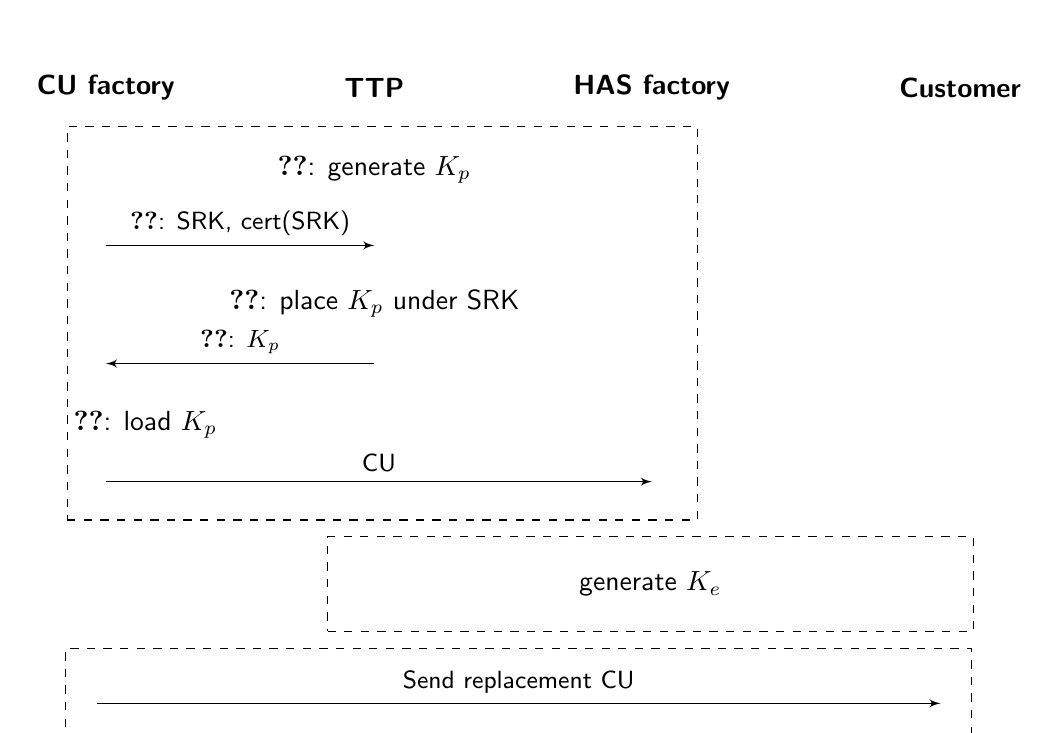
\begin{tikzpicture}[node distance=1.9cm,auto,>=latex',scale=1, every node/.style={scale=1}, font=\sffamily]
		%\def\ts{\footnotesize}
		% Kp things
		\def\ts{\small}
		\node (cu) at (0,0) {\textbf{CU factory}};
		\node[right=of cu] (authority) {\textbf{TTP}};
		\node[right=of authority] (has) {\textbf{HAS factory}};
		\node[right=of has] (customer) {\textbf{Customer}};

		\node[below=0.5cm of authority] (genkey) {\ref{item:genkp}: generate $K_p$};
		\draw[->] ([yshift=-2cm]cu.center) -- node [midway] {\ts \ref{item:sendsrk}: SRK, cert(SRK)} ([yshift=-2cm]authority.center);
		\node[below=2.2cm of authority] (genkey) {\ref{item:migratetocusrk}: place $K_p$ under SRK};		
				
		\draw[<-] ([yshift=-3.5cm]cu.center) -- node [midway] {\ts \ref{item:sendkp}: $K_p$} ([yshift=-3.5cm]authority.center);

		\node (loadblob) at ([xshift=0.5cm,yshift=-4.0cm]cu.south) {\ref{item:culoadblob}: load $K_p$};

		\draw[->] ([yshift=-5.0cm]cu.center) -- node [midway] {\ts CU} ([yshift=-5.0cm]has.center);
		\node (initialization) at ([xshift=-0.5cm, yshift=-0.2cm]cu.south) [draw,dashed,minimum width=8cm,minimum height=5.0cm,anchor=north west] {};
		
		% Generate Ke things
		\node (kegeneration) at ([xshift=-0.7cm, yshift=-0.2cm]initialization.south) [draw,dashed,minimum width=8.2cm,minimum height=1.2cm,anchor=north west] {generate $K_e$};
		
		% Send new CU things
		\node (sendnewcu) at ([xshift=-7.43cm, yshift=-0.2cm]kegeneration.south) [draw,dashed,minimum width=11.5cm,minimum height=1.2cm,anchor=north west] {};
		\draw[->] ([yshift=-0.1cm, xshift=0.4cm]sendnewcu.west) -- node [midway] {\ts Send replacement CU} ([yshift=-0.1cm, xshift=-0.4cm]sendnewcu.east);
	\end{tikzpicture}
	}
	\caption{Overview of the proposed system}
	\label{fig:overviewDesign}
\end{figure}


\begin{enumerate}
\item The TTP generates the CMK key $K_{p}$ to be included in all new TPMs.  \label{item:genkp}
\item The CU manufacturer takes ownership of a new TPM and asks the TTP for $K_p$ to be migrated under the new SRK. \label{item:sendsrk}
\item The TTP migrates the key to the given SRK. \label{item:migratetocusrk}
\item The TTP sends migrated key, encrypted with the SRK public key, to the CU factory. \label{item:sendkp}
\item The CU factory loads the key into the CU. \label{item:culoadblob}
\end{enumerate}

At this point, a generic board has been prepared with a unique SRK, and the $K_p$ which is common for all boards created by the same CU.
The boards are now prepared to be shipped either to a HAS factory for HAS assembly, or to a customer as replacement for a broken board. Assume it has been sent to a HAS factory. The next step is then to generate the customer specific key $K_e$. We consider three different alternatives for generating $K_e$, namely a TTP generated $K_e$, a HAS generated $K_e$, and a customer generated $K_e$. 

Since the boards are generic, we must take two important aspects into account. First, since $K_e$ is a migratable key in TPM 1.2, we must ensure that it can not be migrated further by a malicious customer employee (knowing the owner secret). This can be controlled by not disclosing the migration secret to untrusted users, i.e., simply to destroy it after key generation. In TPM 2.0 this can be controlled more easily by using the fixedParent attribute. Second, we must also ensure that $K_e$ is bound to the HAS, so it can not be used by other customers. This can be done by restricting the use of the key to a given PCR setting. In TPM 1.2, the PCR settings can be directly specified in the key structure, while in TPM 2.0 this is achieved using policies.

\subsection{TTP Generated $K_e$} \label{sec:ttpgeneratedke}
If the $K_e$ is generated by the TTP, the customer needs to send the PCR values which the new key should be bound to. Note that this requires online communication between the two entities. The new key will only be loadable under $K_p$, and only usable on a HAS with the correct PCR values. The steps can be described as in Figure~\ref{fig:ttpgeneratedke}.
\begin{figure}[hbtp]
	\centering
	\resizebox{80mm}{!}{
		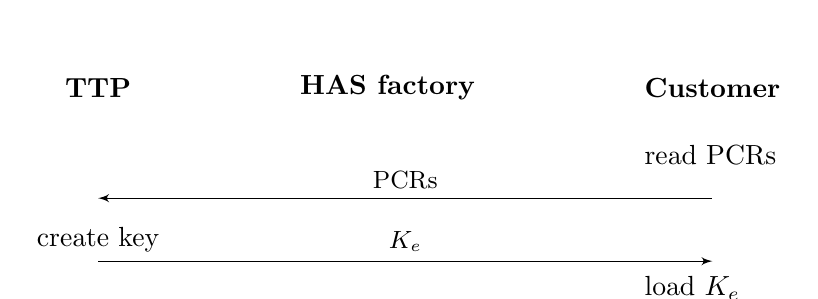
\begin{tikzpicture}[node distance=1.9cm,auto,>=latex',scale=1, every node/.style={scale=1}]
		\def\ts{\small}
		\node at (0,0) (authority) {\textbf{TTP}};
		\node[right=of authority] (has) {\textbf{HAS factory}};
		\node[right=of has] (customer) {\textbf{Customer}};
		
		\node[below left=0.6cm and 0.0cm of customer,right] (readpcrs) {read PCRs};
		\draw[<-] ([yshift=-1.4cm]authority.center) -- node [midway] {\ts PCRs} ([yshift=-1.4cm]customer.center);
		\node[below=1.4cm of authority] (genkey) {create key};		
		
		\draw[->] ([yshift=-2.2cm]authority.center) -- node [midway] {\ts $K_e$} ([yshift=-2.2cm]customer.center);
		
		\node[right] (loadke) at ([yshift=-2.3cm]customer.south west) {load $K_e$};
		\end{tikzpicture}
	}
	\caption{TTP generated $K_e$}
	\label{fig:ttpgeneratedke}
\end{figure}

\subsection{HAS Manufacturer Generated $K_e$} \label{sec:hasgeneratedke}
If the HAS manufacturer generates $K_e$, it can be generated upon HAS assembly. The customer specific key is created on one CU, and then the blob is copied and loaded on the other CU as well. See Figure~\ref{fig:hasgeneratedke} for the executed steps.
\begin{figure}[hbtp]
	\centering
	\resizebox{80mm}{!}{
		
\begin{tikzpicture}[node distance=1.9cm,auto,>=latex',scale=1, every node/.style={scale=1}]
		%\def\ts{\footnotesize}
		% Kp things
		\def\ts{\small}
		\node at (0,0) (authority) {\textbf{TTP}};
		\node[right=of authority] (has) {\textbf{HAS factory}};
		\node[right=of has] (customer) {\textbf{Customer}};
		
		\node[below left=0.5cm and 0.0cm of has,right] (readpcrs) {read PCRs};
		\node[below left=0.9cm and 0.0cm of has,right] (createkey) {create key};
		\node[below left=1.3cm and 0.0cm of has,right] (loadke) {load key};
		\end{tikzpicture}
	}
	\caption{HAS factory generated $K_e$}
	\label{fig:hasgeneratedke}
\end{figure}

\subsection{Customer Generated $K_e$} \label{sec:customergeneratedke}
The customer can execute the same steps as the HAS manufacturer in the section above to generate $K_e$. There is no difference in commands as the hardware is assembled in the same way as when it left the HAS manufacturer. Figure~\ref{fig:customergeneratedke} describes the commands.
\begin{figure}[hbtp]
	\centering
	\resizebox{80mm}{!}{
		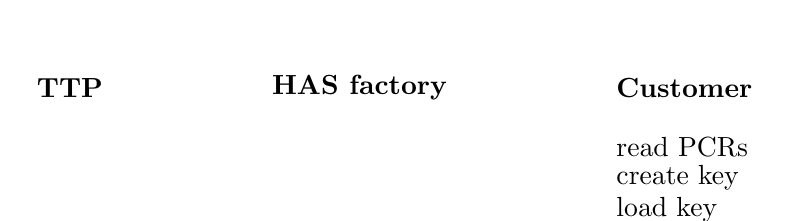
\begin{tikzpicture}[node distance=1.9cm,auto,>=latex',scale=1, every node/.style={scale=1}]
		%\def\ts{\footnotesize}
		% Kp things
		\def\ts{\small}
		\node at (0,0) (authority) {\textbf{TTP}};
		\node[right=of authority] (has) {\textbf{HAS factory}};
		\node[right=of has] (customer) {\textbf{Customer}};
		
		\node[below left=0.5cm and 0.0cm of customer,right] (readpcrs) {read PCRs};
		\node[below left=0.9cm and 0.0cm of customer,right] (createkey) {create key};
		\node[below left=1.3cm and 0.0cm of customer,right] (loadke) {load key};
		\end{tikzpicture}
	}
	\caption{Customer generated $K_e$}
	\label{fig:customergeneratedke}
\end{figure}

\subsection{HAS Initialization}
Before leaving the HAS factory, and before creating the customer-specific keys, the HAS must personalize the HAS in such a way that the PCR values are unique to every customer. This ensures that customer-specific keys can be created.

When the HAS arrives to the customer, the customer must verify that the PCR values after system startup are indeed unique to the customer. This can be done by verifying that the Stored Measurements Log (SML) includes a hash that is customer dependent. If the HAS passes this test, it is ready to be used, knowing that $K_e$ can only be decrypted by this HAS. %For TTP and HAS generated $K_e$, this step is done after the creation of the key and for customer generated $K_e$ this is done prior to the generation of the key.

\section{\texorpdfstring{Security Analysis and Comparison of Properties for $K_e$ Generation}{Security Analysis and Comparison of Properties for Ke Generation}} \label{sec:secanalysis}
We assume that any data that resides on secondary storage on the HAS can be stolen by a malicious employee (\ref{TcustEmployees}). This includes the encrypted sensitive data, the encrypted sensitive part of a TPM protected key, and key usage secrets that are needed to use a key. While it could be possible to restrict the usage secret to only a small number of trusted employees, thus keeping it confidential, or to distribute it using secret sharing, we do not make such assumptions in this work. Since $K_e$ can only be used on a customer specific HAS, the encrypted sensitive part of $K_e$ can only be decrypted on this HAS. Thus, it is not possible to steal the encrypted data and the encrypted $K_e$ and decrypt the data using a generic board. The sensitive data is in clear only in primary memory, when used by the HAS software.

Since the boards are generic, a stolen board will not give an attacker any additional information compared to using their own boards. This mitigates threat~\ref{Tstolen}.

Threat \ref{THAS} can be mitigated to different extent depending on which $K_e$ generation alternative is used and which TPM version is used. When using a TTP for $K_e$ generation or when $K_e$ is generated by the customer, the HAS manufacturer employees will have no access to $K_e$ or any information about it. If $K_e$ is generated by the HAS manufacturer, for TPM 1.2, the security depends on the migration secret being destroyed after the key is generated. Otherwise, this key could be leaked to a malicious customer which is able to migrate $K_e$ outside the TPM. In TPM 2.0, $K_e$ is created with fixedParent set, which can be verified by the customer when the HAS is being initialized. Thus, it is only for HAS manufacturer created keys in TPM 1.2 that we are not able to fully mitigate \ref{THAS}, but it can be noted that an attack require cooperation between HAS manufacturer and customer employees. Returning to \ref{TcustEmployees}, we can also note that for customer created $K_e$ in TPM 1.2, we must ensure that the migration secret is destroyed. Thus, for TPM 1.2, higher security is achieved when $K_e$ is generated by a trusted third party. A summary of the different properties for different cases are given in Table~\ref{tbl:kesecanalysis}.

We note that there are three parts required to gain access to the secure information stored in the HAS: the encrypted data, the customer-specific key $K_e$, and the HAS itself. Thus, we cannot protect against cases where an attacker gets hold of all three of these parts. This includes a potential case where a malicious HAS employee cooperates with an malicious company employee at company A. If they have access to both stolen encrypted data, and the stolen $K_e$ from another company B, the HAS manufacturer and employee at A may cooperate to build a HAS with the same customer-specific PCR values as customer B, thus enabling them to decrypt the stolen data.

Finally, we also note that our analysis relies on the assumption that the TTP is trusted and available.

%\newcommand{\ayemark}{$\text{\rlap{$\checkmark$}}\square$}
\newcommand{\ayemark}{$\boxtimes$}
\newcommand{\nopemark}{$\square$}
%\newcommand{\ayemark}{OK}
%\newcommand{\nopemark}{X}

\begin{table}[hbtp]
	\begin{center}
		\caption{A summary of the properties when different entities generate the key $K_e$}
		\label{tbl:kesecanalysis}
		\begin{tabular}{m{3.65cm}l cc l cc l cc}
			\toprule
			& \phantom{w} & \multicolumn{2}{c}{TTP} & \phantom{w} & \multicolumn{2}{c}{HAS man.} & \phantom{w} & \multicolumn{2}{c}{Customer} \\
			\cmidrule{3-4} \cmidrule{6-7} \cmidrule{9-10}
			&& 1.2~~ & 2.0 & & 1.2 & 2.0 & & 1.2 & 2.0 \\
			\midrule
			{\small No online communication with other entity needed.}& & \nopemark & \nopemark && \ayemark & \ayemark && \ayemark & \ayemark \\
			\midrule
			{\small Possible to verify that $K_e$ is bound to $K_p$.}& & \ayemark & \ayemark && \nopemark & \ayemark && \nopemark & \ayemark \\
			\bottomrule
		\end{tabular}
	\end{center}
\end{table}

\section{Unified API} \label{sec:unifiedapi}

We have developed a unified API for the proposed functionality, such that a move from TPM 1.2 to TPM 2.0 will be as simple as possible.
By looking at the different phases of our solution, we can construct sequences of TPM commands for each of the two TPM versions, such that we get the same behaviour, abstracting away the differences between the TPM versions.

The API has been implemented and tested to ensure the correctness of the given commands, both for TPM 1.2 and TPM 2.0.
To do this, two different TPM simulators and support libraries have been used, one for each TPM version.

For TPM 1.2, IBM's Software TPM version 4720 \cite{ibmswtpm} has been used, which also includes \texttt{libtpm}, which can be used to interface with the simulator.
For TPM 2.0, Microsoft's TPM2 Simulator version 1.1 \cite{mstpm2sim} has been used, together with Microsoft's TPM Software Stack version 1.1 \cite{mstssmsr11}.

\subsection{Generation and Migration of $K_p$} \label{sec:unifiedapikp}

The first step in Figure~\ref{fig:overviewDesign} is to generate $K_p$. The following steps are executed on the TTP:
\begin{center}
	\begin{minipage}{0.4\linewidth}
		\begin{center}
			TPM 1.2
		\end{center}
		\begin{tpmcommands}
			\begin{verbatim}
			TPM_CMK_ApproveMA
			TPM_CMK_CreateKey
			\end{verbatim}
		\end{tpmcommands}
	\end{minipage}
	~~~~~~~~
	\begin{minipage}{0.4\linewidth}
		\begin{center}
			TPM 2.0
		\end{center}
		\begin{tpmcommands}
			\begin{verbatim}
			TPM2_PolicyAuthorize
			TPM2_Create
			\end{verbatim}
		\end{tpmcommands}
	\end{minipage}
\end{center}

In step~\ref{item:sendsrk}, the CU factory sends the SRK to the TTP, which then in step~\ref{item:migratetocusrk} executes the following commands to create a blob which is decryptable under the given CU's SRK.
\begin{center}
	\begin{minipage}{0.4\linewidth}
		\begin{center}
			TPM 1.2
		\end{center}
		\begin{tpmcommands}
			\begin{verbatim}
			TPM_AuthorizeMigrationKey
			TPM_CMK_CreateTicket
			TPM_CMK_CreateBlob
			\end{verbatim}
		\end{tpmcommands}
	\end{minipage}
	~~~~~~~~
	\begin{minipage}{0.4\linewidth}
		\begin{center}
			TPM 2.0
		\end{center}
		\begin{tpmcommands}
			\begin{verbatim}
			TPM2_LoadExternal
			TPM2_PolicyDuplicationSelect
			TPM2_PolicyAuthorize
			TPM2_Duplicate
			\end{verbatim}
		\end{tpmcommands}
	\end{minipage}
\end{center}

In step~\ref{item:sendkp}, the blob is sent to the CU factory, which then loads the blob into the TPM under the SRK (step~\ref{item:culoadblob}):
\begin{center}
	\begin{minipage}{0.4\linewidth}
		\begin{center}
			TPM 1.2
		\end{center}
		\begin{tpmcommands}
			\begin{verbatim}
			TPM_CMK_CreateTicket
			TPM_CMK_ConvertMigration
			TPM_LoadKey2
			\end{verbatim}
		\end{tpmcommands}
	\end{minipage}
	~~~~~~~~
	\begin{minipage}{0.4\linewidth}
		\begin{center}
			TPM 2.0
		\end{center}
		\begin{tpmcommands}
			\begin{verbatim}
			TPM2_Import
			TPM2_Load
			\end{verbatim}
		\end{tpmcommands}
	\end{minipage}
\end{center}

The CU now has $K_p$ loaded directly beneath the SRK, and the customer-specific key $K_e$ can be generated.

\subsection{Generation of $K_e$}
The customer-specific key $K_e$ can be generated using any of the alternatives given in Section~\ref{sec:ttpgeneratedke}, \ref{sec:hasgeneratedke}, and \ref{sec:customergeneratedke}.
The commands for each of the three cases are given below:

\subsubsection{TTP Generated $K_e$}
\begin{center}
	\begin{minipage}{0.4\linewidth}
		\begin{center}
			TPM 1.2
		\end{center}
		\begin{tpmcommands}
			\begin{verbatim}
			TPM_PcrRead       // customer
			// send PCRs TTP
			TPM_CreateWrapKey // TTP
			// send blob to customer
			TPM_LoadKey2      // customer CU1
			TPM_LoadKey2      // customer CU2
			\end{verbatim}
		\end{tpmcommands}
	\end{minipage}
	~~~~~~~~
	\begin{minipage}{0.4\linewidth}
		\begin{center}
			TPM 2.0
		\end{center}
		\begin{tpmcommands}
			\begin{verbatim}
			TPM2_PCR_Read  // customer
			// send PCRs to TTP
			TPM2_PolicyPCR // ttp
			TPM2_Create    // ttp
			// send blob to customer
			TPM2_Load      // customer CU1
			TPM2_Load      // customer CU2
			\end{verbatim}
		\end{tpmcommands}
	\end{minipage}
\end{center}


\subsubsection{HAS Manufacturer Generated $K_e$}
\begin{center}
	\begin{minipage}{0.4\linewidth}
		\begin{center}
			TPM 1.2
		\end{center}
		\begin{tpmcommands}
			\begin{verbatim}
			TPM_PcrRead       // CU1
			TPM_CreateWrapKey // CU1
			TPM_LoadKey2      // CU1
			// copy blob to other CU
			TPM_LoadKey2      // CU2
			\end{verbatim}
		\end{tpmcommands}
	\end{minipage}
	~~~~~~~~
	\begin{minipage}{0.4\linewidth}
		\begin{center}
			TPM 2.0
		\end{center}
		\begin{tpmcommands}
			\begin{verbatim}
			TPM2_PCR_Read  // CU1
			TPM2_PolicyPCR // CU1
			TPM2_Create    // CU1
			TPM2_Load      // CU1
			// copy blob to other CU
			TPM2_Load      // CU2
			\end{verbatim}
		\end{tpmcommands}
	\end{minipage}
\end{center}

\subsubsection{Customer Generated $K_e$.}
These are the same commands as used when the HAS manufacturer generates $K_e$, the only difference is that they are now executed by the customer.
\begin{center}
	\begin{minipage}{0.4\linewidth}
		\begin{center}
			TPM 1.2
		\end{center}
		\begin{tpmcommands}
			\begin{verbatim}
			TPM_PcrRead       // CU1
			TPM_CreateWrapKey // CU1
			TPM_LoadKey2      // CU1
			// copy blob to other CU
			TPM_LoadKey2      // CU2
			\end{verbatim}
		\end{tpmcommands}
	\end{minipage}
	~~~~~~~~
	\begin{minipage}{0.4\linewidth}
		\begin{center}
			TPM 2.0
		\end{center}
		\begin{tpmcommands}
			\begin{verbatim}
			TPM2_PCR_Read  // CU1
			TPM2_PolicyPCR // CU1
			TPM2_Create    // CU1
			TPM2_Load      // CU1
			// copy blob to other CU
			TPM2_Load      // CU2
			\end{verbatim}
		\end{tpmcommands}
	\end{minipage}
\end{center}

\subsection{CU Failure}

In the event of a CU failure, the customer will receive a new CU directly from the CU factory. This will have the key $K_p$ loaded, as per the steps described in Section~\ref{sec:unifiedapikp}. The customer will however be required to load the customer-specific key $K_e$. Since the key is located beneath the common key $K_p$ in the key hierarchy, the same key blob that is used on the other CU can be used directly on the new CU. Thus, the key blob of $K_e$ is copied to the new CU, and the following commands are executed:
\begin{center}
	\begin{minipage}{0.4\linewidth}
		\begin{center}
			TPM 1.2
		\end{center}
		\begin{tpmcommands}
			\begin{verbatim}
			TPM_LoadKey2
			\end{verbatim}
		\end{tpmcommands}
	\end{minipage}
	~~~~~~~~
	\begin{minipage}{0.4\linewidth}
		\begin{center}
			TPM 2.0
		\end{center}
		\begin{tpmcommands}
			\begin{verbatim}
			TPM2_Load
			\end{verbatim}
		\end{tpmcommands}
	\end{minipage}
\end{center}

\section{Related Work} \label{sec:tpmhas:relatedwork}
%THIS MUST BE EXAPANDED\\\\
Though there are few examples of widely adopted applications taking advantage of TPM functionality, several use cases have been considered before. In~\cite{wagan:2010,guette:2008}, the use of TPMs to secure VANETs was proposed and studied. Using TPMs to increase the security in RFID tags and NFC communication has also been proposed in~\cite{mubarak:2010} and~\cite{hutter:2010} respectively.

The use of Certifiable Migration Keys in the Mobile Trusted Module (MTM) for protecting secret data was proposed in~\cite{kang:2009}.

Today, virtualization is a growing area, and there have been several different proposals on how to use the TPM in virtual machines. In \cite{berger:2006} a complete virtualized TPM module is developed, which is then linked to the hardware TPM. In \cite{england:2008} a para-virtualized solution is discussed. \cite{sadeghi:2008} discusses yet another design, and also discusses migration of virtual TPMs to a large extent.

The use of TPMs in cloud computing has also been considered in recent years. In \cite{santos:2009} secure launch and migration of VMs in the cloud is discussed in the context of trusted computing, and in \cite{aslam:2012} secure migration of virtual machines through the use of the Trusted Platform Module is further discussed.

Use of remote attestation has been considered in many works before \cite{berger:2006,gu:2008,nauman:2010,sailer:2004}. In remote attestation, the goal is to provide the contents of PCRs to a remote party. The PCR values are signed with an AIK and the remote party can verify through the signature that the system is in a known configuration. Using an SML, the content of this, which is a set of run programs and their hashes, can be compared to the signed PCR values. In our work, it is the customer that verifies the PCRs and the SML.

\section{Conclusions} \label{sec:conc}
We have proposed a solution for using TPMs to secure sensitive data in a high availability system. The main challenge is to create customers specific keys which can only be used in the customer's own HAS, while at the same time allowing generic computational units to be produced and shipped as replacement boards. Since employees come and go, we also do not want to trust employees. Our proposed solution relies on binding the customer specific key to a parent key which is the same on all boards, and to also bind the key to PCR values that are specific to a customer. We show that the increased functionality in TPM 2.0 allows a more secure solution in certain cases. In addition to the proposed solution we define an API such that it is possible to upgrade from TPM 1.2 to TPM 2.0 without changing the communication flow.

\subsubsection{Acknowledgments.}The authors would like to thank the anonymous reviewers for their valuable comments.

{\raggedright
	\printbibliography[segment=\therefsegment,heading=subbibliography]
}

}
\fi

\ifpaperII
\newrefsegment
\addtolength{\apa}{2cm}
\fancyhead[RE]{\paperref{ch:tpm12to20}: \paperIItitle}
\chapter[\paperIItitle]{\texorpdfstring{%
		\paperIItitle}{%
		\paperIItitle}}
\label{ch:tpm12to20}
\paperRemark{\paperIIref}

% CHANGES: fixed wrong reference, original paper links to bitlocker but link goes to virtual smartcards.
%      ACTION: replace with new bitlocker reference used in other parts of paper.

{
%\documentclass{llncs}
%%\documentclass[conference]{IEEEtran}
%\usepackage{multirow}
%\usepackage{rotating}
%\usepackage{tikz}
%\usetikzlibrary{arrows,backgrounds,positioning,matrix}
%\usepackage{enumitem}
%\usepackage{hyperref}
%\hypersetup{pdfborder=0 0 0}
%\usepackage{listings}
%\usepackage{booktabs}
%\usepackage{array}
%\usepackage{amsmath}
%\usepackage{amssymb}
%\usepackage{color}
%\usepackage{subcaption}
%\newcolumntype{P}[1]{>{\centering\let\newline\\\arraybackslash\hspace{0pt}}m{#1}}
%\usepackage{geometry}
%
%\makeatletter
%\let\orgdescriptionlabel\descriptionlabel
%\renewcommand*{\descriptionlabel}[1]{%
%	\let\orglabel\label
%	\let\label\@gobble
%	\phantomsection
%	\edef\@currentlabel{#1}%
%	%\edef\@currentlabelname{#1}%
%	\let\label\orglabel
%	\orgdescriptionlabel{#1}%
%}
%\makeatother

\renewcommand{\sectionautorefname}{Section}
\renewcommand{\subsectionautorefname}{\sectionautorefname}
%\renewcommand{\subsubsectionautorefname}{\sectionautorefname}

\newenvironment{tpmcommands}{\begin{scriptsize}}{\end{scriptsize}}

\newcommand{\tpms}{TPM$_{\text{S}}$}
\newcommand{\tpma}{TPM$_{\text{A}}$}
\newcommand{\tpmd}{TPM$_{\text{D}}$}
\newcommand{\ek}{$K$}
\newcommand{\eksib}{$K_\text{sib}$}
\newcommand{\ca}{TPM$_{\text{C}}$}
\newcommand{\tpmc}[1]{\texttt{#1}}
\newcommand{\tpmco}[1]{\tpmc{TPM\_#1}}
\newcommand{\tpmct}[1]{\tpmc{TPM2\_#1}}
\newcommand{\todo}[1]{\textcolor{red}{\textbf{#1}}}
\def\policychainscalefactor{0.8}

\section*{Abstract}
We consider the problem of migrating keys from TPM 1.2 to the backwards
incompatible TPM 2.0. The major differences between
the two versions introduce several challenges for deployed systems when
support for TPM 2.0 is introduced. We show how TPM 2.0 support can be
introduced while still maintaining the functionality specified by TPM 1.2,
allowing a smoother transition to the newer version. Specifically, we
propose a solution such that keys can be migrated from TPM 1.2 to TPM 2.0,
while retaining behavior with regard to e.g. authorization, migration
secrets, PCR values and CMK functionality. This is achieved by utilizing
new functionality, such as policies, in TPM 2.0. The proposed solution is
implemented and verified using TPM emulators to ensure correctness.

\section{Introduction}
There are different versions of the TPM, which differ from one another in several ways. In this paper we consider TPM 1.2, introduced in 2003, and TPM 2.0 which was introduced in 2012. TPM 2.0 is not backwards compatible with TPM 1.2, but nevertheless TPM 2.0 chips are now available \cite{infineon-tpm20-released} and have started to ship in devices \cite{infineon-tpm20-surfacepro}. %and it is likely that some years in the future, TPM 2.0 will be the predominant version in new equipment.

We consider the process of migrating from the TPM 1.2 generation chips, to the newer TPM 2.0. As new equipment comes with TPM 2.0 chips, we want to be able to move or copy keys from TPM 1.2 to the new chips, while still maintaining the same functionality. However, because of the lack of backwards compatibility, there is no such support built into the TPM specifications. This presents a problem when we would like to use the same keys even when moving to a newer TPM, for example to be able to decrypt previously encrypted data. In addition, we may want to continue to use these keys with the same functionality, despite the differences between the specifications.

The lack of backwards compatibility means that this migration has to be done manually. Keys have to be converted between different formats, and adapted to the different feature sets of the two standards. Some features in TPM 1.2 have no direct equivalent in TPM 2.0, but identical or similar behavior can be achieved by using new features of TPM 2.0.
%The goal of this paper is to give a solution on how to achieve this for several different cases.
The goal of this paper is to give a solution for how to achieve this for all different key types and migration alternatives in TPM 1.2.
As an example, in TPM 1.2 there is a concept of a \emph{migration secret}, which authorizes the migration of a key to another TPM. This migration secret has no direct counterpart in TPM 2.0, but the same behavior can be implemented using functionality only available in the TPM 2.0 specifications.
Another example is the use of Certifiable Migratable Keys (CMKs) in TPM 1.2, which also requires a non-trivial design by expressing the functionality as policies in TPM 2.0.

We describe a process which allows us to migrate keys from a TPM 1.2 to a TPM 2.0. We start by determining a set of requirements, and present a solution which performs migration according to the presented requirements.
We start by implementing the equivalent functionality of TPM 1.2's migration secret in TPM 2.0, using constructions only available in the newest TPM version. We then look at keys bound to Platform Configuration Register (PCR) values, and present a way to handle the incompatibilities in key format between TPM 1.2 and TPM 2.0. We also present a solution for CMKs, such that equivalent behavior is achieved in both TPM versions.
We do not consider the case of TPM 2.0 to 1.2 migration, since it is not likely that new TPM 1.2 equipment will be deployed once equipment with TPM 2.0 has been deployed.

The paper is organized as follows. \autoref{sec:tpm12to20:overview} presents a brief overview of TPM 1.2 and 2.0. In \autoref{sec:goals} we present our goals and requirements. In \autoref{sec:scenarios} we describe our proposed solution for different relevant scenarios, which are then extended to the case of CMKs in \autoref{sec:cmks}. \autoref{sec:tpm12to20:implementation} describes the implementation. Finally in \autoref{sec:tpm12to20:relatedwork}, we discuss some related work. \autoref{sec:discussion} concludes the paper.

\section{Overview of TPM 1.2 and TPM 2.0} \label{sec:tpm12to20:overview}
This section will give a short introduction to TPM 1.2 and 2.0, with focus on issues related to key migration. For a complete review, consult the specifications \cite{TPM1.2spec,TPM2.0r16}.

\subsection{Overview of TPM 1.2 and Certifiable Migratable Keys}
A TPM 1.2 provides a key hierarchy of asymmetric keys. Keys can be of different types, for example storage keys, signing keys, or decryption keys (the last called binding key in TPM 1.2). Since the keys are asymmetric, they consist of two parts: one public and one private part. The private part of every key is encrypted with the public part of the parent key. Only a storage key can be the parent of another key.

Certain operations on the TPM, e.g. some commands related to migration, must only be performed by the TPM owner. These operations are authorized by proving knowledge of an \emph{owner secret}, which is set when someone takes ownership of the TPM. To be able to use the private part of a key, e.g. to decrypt or sign data, the user must provide a \emph{usage secret}. This secret is stored inside the key in the TPM, and can be unique for each key.

Copying keys between different TPMs is called \emph{migration}, and was introduced in TPM 1.1\cite{TPM1.1bspec}. To authorize such an operation the TPM owner must first authorize the destination using the command \tpmco{AuthorizeMigrationKey}. We note that the TPM owner can authorize any destination, thus making it possible to migrate the key to any TPM, or even to a keypair generated outside any TPM. In addition, the user performing the migration must prove knowledge of the \emph{migration secret}, which is a secret set on key creation. If this secret is not known, the key is not migratable. This is verified during execution of \tpmco{CreateMigrationBlob}, which outputs a data blob which can be transferred to the destination TPM. At the destination, the key can be loaded by \tpmco{LoadKey2}, possibly after conversion by \tpmco{ConvertMigrationBlob}.

In TPM 1.2, CMKs were introduced. Their migration is further restricted, such that instead of the migration secret above, an authorization from a trusted entity, called the Migration Selection Authority (MSA), is required. The MSAs are chosen at key creation time. During the migration, the MSA must approve the destination, either implicitly by migrating the key to the MSA itself, or by signing a ticket containing the destination. The signature is done using the private key of the MSA. By signing the ticket, the MSA approves the migration of the specified key to a specific destination. This signature is required by the source TPM to actually perform the migration.

\subsection{Overview of TPM 2.0}
In TPM 2.0 the asymmetric key hierarchy has been generalized, and has been replaced with an object hierarchy. Objects can be asymmetric or symmetric keys, or data blobs. The type of the object is determined by a set of flags on the object: \emph{sign}, \emph{decrypt}, and \emph{restricted}. An object with the flags \emph{decrypt} and \emph{restricted} set is a storage key, since it can be used to encrypt and decrypt the private parts of child keys, and the \emph{restricted} bit tells the TPM to operate only on data prepared by the TPM (for example keys). However, the storage keys in TPM 2.0 protect its child keys by using symmetric encryption instead of asymmetric. The symmetric key is derived from a seed included in the key itself. In addition to this, TPM 2.0 allows for a wide range of ciphers and algorithms, including different symmetric ciphers and hash functions.

In TPM 2.0, migration has been renamed to \emph{duplication}. Indeed, this is a more appropriate terminology, since keys are not removed from the source when performing a migration. Instead the key will exist in both TPMs. There are two flags connected to the duplicability of a key: \emph{fixedTPM} and \emph{fixedParent}. A key with fixedTPM set can never leave the TPM, and can thus not be duplicated. The other flag, fixedParent, tells us if the key is fixed to its parent. If the flag is set, the key cannot be explicitly duplicated, but it may still be loaded in another TPM if it is possible to duplicate its parent.

Just like in TPM 1.2, use of the private part of a key requires a usage secret, but there is no direct equivalent of the migration secret. Instead, a more general authorization mechanism has been introduced in TPM 2.0, namely policies.

\subsection{Policies in TPM 2.0}
A major addition in TPM 2.0 is the introduction of policies. A policy can be used to authorize different operations on an object in the hierarchy. The policy is set at creation time, by including a value \tpmc{authPolicy} in the object. This value is created by repeatedly hashing different values from different policy commands. Possible commands are for example policies based on time, signatures, or secret values. Different policies can also be combined using OR.

Before executing a command using the object, a policy hash must be built in a policy session. The session also includes context specific values which are checked during command execution, for example if we are authorizing duplication or usage of the object, or what authorization method to use. The resulting policy hash of the policy session is then compared to the \tpmc{authPolicy} in the object to authorize the command execution.

In this paper we are mostly concerned with duplication and authorization. Thus, we are only interested in a subset of the different policy commands:

\begin{itemize}
	\item \tpmct{PolicyAuthValue} requires the usage secret of the object being authorized, and does the authorization using a HMAC.
	\item \tpmct{PolicyAuthorize} allows us to modify an existing policy. A new policy is signed using the private key of an authority, and if this signature is valid, the policy is included in the policy session.
	\item \tpmct{PolicyCommandCode} limits the authorization to a certain command, for example to authorize duplication only. This is done by setting a \emph{command code} in the current policy session.
	\item \tpmct{PolicyDuplicationSelect} limits the allowed destination parent when performing a duplication.
	\item \tpmct{PolicyOR} is a logical OR policy, which is true if the current policy hash matches any of the conditions in this policy.
	\item \tpmct{PolicyPassword} requires the usage secret of the object being authorized, and does the authorization using the password in clear.
	\item \tpmct{PolicyPCR} requires the PCRs (see \autoref{sec:pcrs}) to have a specific set of values.
	\item \tpmct{PolicySecret} requires the usage secret of another object on the TPM.
	\item \tpmct{PolicySigned} requires a digital signature.
\end{itemize}

\subsection{Platform Configuration Registers} \label{sec:pcrs}
Both TPM 1.2 and 2.0 have a number of Platform Configuration Registers (PCRs). Each PCR stores a hash value, which is created by repeatedly calling \tpmco{Extend} or \tpmct{Extend}. The extend operation depends both on the previous PCR value, and on the new data. This can be used to store measurements of hardware configuration and software on the host. Keys in both TPM 1.2 and 2.0 can be bound to PCR values, such that the use of a key requires certain PCRs to be in a specified state. This ensures that such keys are only usable in a known environment. In addition, the PCR values can be read by using the commands \tpmco{PCRRead} and \tpmct{PCR\_Read}.

\subsection{Comparing Migration in TPM 1.2 and TPM 2.0}
%As can be seen from the previous descriptions, there are multiple differences when it comes to migration between the two TPM versions.
From the descriptions above we see that when it comes to migration, there are several differences between the two TPM versions.

To perform a migration of a (non-CMK) TPM 1.2 key, the following criteria must be fulfilled:

\begin{enumerate}
	\item The key must have been created with the key flag \texttt{migratable} set to TRUE.
	\item The migration secret must be known.
	\item The TPM owner must authorize the migration destination.
	\item The usage secret of the parent key on the source TPM must be known.
	\item The usage secret of the parent key on the destination TPM must be known.
\end{enumerate}

In comparison, the following criteria must be fulfilled when migrating a TPM 2.0 key:

\begin{enumerate}
	\item The key must have \tpmc{fixedParent} CLEAR.
	\item The command code of the policy session must be \tpmc{TPM\_CC\_Duplicate}, i.e. the key must have a policy which allows for duplication.
	\item The usage secret of the parent key on the source TPM must be known.
	\item The usage secret of the parent key on the destination TPM must be known.
\end{enumerate}

We first note the similarities, namely that for both TPM versions, the usage secret of the  parent key on the source TPM must be known, such that the key to be migrated can be loaded into the TPM. In addition, the usage secret of the destination TPM's parent key must also be known, such that the key to be migrated can be added as a child key.

In TPM 1.2 there is an explicit flag which tells whether or not the key is migratable. This is not the case in TPM 2.0, where there are two flags which control the migratability of a key. If \tpmc{fixedParent} is SET, then the key has a fixed parent, and cannot be migrated directly (however, it could still be migrated if its parent is migratable). If \tpmc{fixedTPM} is SET, the key can never be migrated. We note that it is not possible to create a key with \tpmc{fixedParent} CLEAR and \tpmc{fixedTPM} SET, so a sufficient condition is that \tpmc{fixedParent} is CLEAR.

Another difference is the authorization of the migration. In TPM 1.2 this is done by proving knowledge of the migration secret. In TPM 2.0, it is done with a policy session that authorizes the migration. We note that the policy session is a more generic approach, which supports multiple ways of authorizing the migration through the use of any policy command. The only requirement is that there exists a command in the chain of policy commands that explicitly sets the commandCode to \tpmc{TPM\_CC\_Duplicate}, since duplication is a special authorization role in TPM 2.0.

%For CMKs in TPM 1.2, the MSA is responsible for ensuring that the destination TPM is valid

Finally, we note that there is no requirement for owner authorization when performing a migration in TPM 2.0.

Looking at the migration of a CMK in TPM 1.2, the following criteria must be fulfilled:

\begin{enumerate}
	\item The MSA must authorize the migration destination.
	\item The TPM owner must authorize the migration destination.
	\item The usage secret of the parent key on the source TPM must be known.
	\item The usage secret of the parent key on the destination TPM must be known.
\end{enumerate}

Compared to the non-CMK criteria described above, the migration secret criterion is replaced by the approval of the MSA. TPM 2.0 does not have the concept of CMKs, but the behavior can be implemented by the use of policies. Details will be presented later in \autoref{sec:cmks}.

\section{Goals} \label{sec:goals}
We want to migrate a \emph{migratable} key from a source TPM (TPM 1.2), hereafter called \tpms{}, to a destination TPM (TPM 2.0), denoted \tpmd{}. The key to be migrated from \tpms{} to \tpmd{} is denoted \ek{}.

If the source key is a CMK, then the migration must also be approved by an already existing trusted third-party, called the authority/MSA. This third party may, or may not, have a TPM module installed, but let's assume that this is the case, and call this party \tpma{}.

When migrating a key between two TPMs of the same version (i.e. either 1.2 $\rightarrow$ 1.2, or 2.0 $\rightarrow$ 2.0) we can immediately import the binary migration blobs produced by the source TPM into the destination TPM. We can also be sure that all features are supported. However, when we do a migration from 1.2 $\rightarrow$ 2.0 the migration blob must be converted manually, taking into account the differences between the two versions.

We introduce a \emph{conversion authority} which is a trusted entity that performs the actual binary conversion between 1.2 and 2.0, and denote this with \ca{}.

Introducing this trusted entity does not lower the security of our proposed solution. If the key \ek{} is a CMK, there is already a trusted third-party (the authority/MSA). If a new, separate, conversion authority is undesirable, it would be possible to extend the MSA to also be the conversion authority.

In the case of a non-CMK, the source key owner is in full control of \ek{}. This means that the owner may migrate it to any destination, including a destination outside of a TPM. Thus the owner has full responsibility and opportunity to choose a trusted conversion authority. It is possible to have the conversion authority on either the source or destination, a separate third system is not required. Seeing the conversion authority as a separate entity does however provide a clear separation of concerns, and simplifies reasoning in this paper.

\subsection{Requirements}
We want our solution to maintain the same functionality with respect to authorization when moving from TPM 1.2 to TPM 2.0. Thus, if an entity is authorized to migrate or use a key at the source TPM, it should have the possibility and authorization to do so also at the destination TPM.

To maintain the functionality when moving between the different TPMs, we identify a number of requirements which must be supported by the conversion authority.

\begin{enumerate}[label=R\arabic*.,ref=R\arabic*]
	\item Keep the same private and public part of the RSA key, such that it can be used to decrypt previously encrypted data, or create identical signatures. \label{req:privpub}
	\item Keep the same authorization requirements for key usage.\label{req:usageath}
	\item Keep the same authorization requirements for key migration. \label{req:migrationauth}
	\item If a key requires a certain state (PCR values) of the TPM, the same state should be required after migration. \label{req:pcr}
	\item Support all key types of the TPM 1.2, i.e., signing, decryption, and storage keys. Both non-CMK and CMK keys should be supported. \label{req:keytypes}
	\item Once migrated to a TPM 2.0, it should be possible (if authorized) to further migrate the key to another TPM 2.0. \label{req:furthermigration}
	\item The migration should be deterministic, such that if the same key is migrated twice, the result at the destination TPM should be identical after both migrations. \label{req:deterministic}
\end{enumerate}

The motivation for \ref{req:deterministic} is that when migrating a storage key in TPM 1.2 or TPM 2.0, its child keys are implicitly migrated as well, since they can just be loaded at the destination TPM with the respective Load-commands. This allows a hierarchy to be moved incrementally, simply by moving the child keys to the destination. However, when migrating keys between TPM 1.2 and 2.0, we will have to perform a conversion step. To be able to perform the migration incrementally at different occasions, the steps involved must be deterministic.

\section{Migration Scenarios} \label{sec:scenarios}
We will look at the following different migration scenarios:

\begin{enumerate}
	\item Migration of a simple, single, key from \tpms{} to \tpmd{}. Only signing keys and decryption keys, without considering PCR values. %, \autoref{sec:simple}.
	\item Migration of a simple, single, key requiring specific values of the PCRs.
	\item Migration of a storage key, including its child keys.
	\item All of the scenarios above, for CMKs.
\end{enumerate}

\subsection{Signing or Decryption Key} \label{sec:simple}
In this case we want to migrate a signing or decryption key from \tpms{} to \tpmd{}. Clearly we must retain both the private and public portions of the key when migrating to \tpmd{}. Furthermore we assume that this key is the child key of the \emph{storage root key} (SRK), but the steps will be identical for any parent key.

Because of the differences between TPM 1.2 and 2.0, both in functionality and in the actual binary migration blob format, we must do a conversion of the binary migration blob before importing it into \tpmd{}. This means that we cannot simply perform the migration to the SRK of \tpmd{}. If we did, the migration blob could only be decrypted by the destination TPM, which would also have to perform the actual conversion. This is not possible, since the conversion cannot be performed inside the destination TPM. Rather, we must use the previously introduced conversion authority, \ca{}. The conversion authority has its own RSA keypair, which will act as an intermediate destination during the migration.

The outline of the conversion is as follows, also depicted in \autoref{fig:conversionoverview}.

\begin{enumerate}
	\item The owner of \tpms{}, and the owner of \ek{} authorize the migration of \ek{} to \ca{}, by proving knowledge of the owner secret and migration secret respectively.
	\item A migration blob is created by the command \tpmco{CreateMigrationBlob}.
	\item The migration blob is first decrypted by \ca{}, and then converted to a TPM 2.0-format, and migrated to the final destination \tpmd{}.
	\item \tpmd{} imports the migration blob and now has its own copy of \ek{}.
\end{enumerate}

%% SUITABLE FOR IEEE double column.
%\begin{figure}[thbp] 
%	\centering
%	\begin{tikzpicture}[node distance=0.6cm,auto,>=latex',scale=0.8, every node/.style={scale=0.8}]
%	% tpm 1.2 (tpms)
%	\node[draw] (parent) at (0,0) {Parent 1};
%	
%	% % % % % % % %
%	
%	% conversion authority (tpmc)
%	\node[draw,right=1.0cm of parent] (parentC) {Parent 2};
%	\node[draw,right=1.0cm of parentC] (parentC2) {Parent 3};
%	
%	\node[draw,below=of parentC,align=left] (tpm12migblob) {TPM 1.2\\migration\\blob};
%	\node[draw,align=left] at (parentC2 |- tpm12migblob) (tpm20keyC) {TPM 2.0\\key};
%	
%	\draw[->] (parentC) to (tpm12migblob);
%	\draw[->] (parentC2) to (tpm20keyC);
%	
%	% box around all tpmc
%	\node[above right=0.3cm and -1.2cm of parentC] {Conversion authority (\ca{})};
%	\draw[dotted] ([xshift=-1.1cm,yshift=1cm]parentC.north) rectangle ([xshift=1.1cm,yshift=-.5cm]tpm20keyC.south);
%	
%	% % % % %
%	% tpm 1.2 again
%	
%	\node[draw] at (parent |- tpm12migblob) (key) {\ek{}}; % use parent X and tpm12migblob Y coord.
%	\draw[->] (parent) to (key);
%	
%	% box around all tpms
%	\node[above=0.3cm of parent] {TPM 1.2 (\tpms{})};
%	\draw[dotted] ([xshift=-1.3cm,yshift=1cm]parent.north) rectangle ([xshift=1.3cm,yshift=-0.7cm]key.south);
%	
%	% % % % % % %
%	
%	% tpm 2.0
%	\node[draw,right=1.0cm of parentC2] (parent2) {Parent 4};
%	\node[draw] at (parent2 |- tpm20keyC) (key2) {\ek{}};
%	
%	\draw[->] (parent2) to (key2);
%	
%	% box around all tpm 2.0
%	\node[above=0.3cm of parent2] {TPM 2.0 (\tpmd{})};
%	\draw[dotted] ([xshift=-1.3cm,yshift=1cm]parent2.north) rectangle ([xshift=1.3cm,yshift=-0.7cm]key2.south);
%	
%	% mapping between entities.
%	\draw[->,dashed] (key.east) to node {migrate} (tpm12migblob.west);
%	\draw[->,dashed] (tpm12migblob.east) to node {convert} (tpm20keyC.west);
%	\draw[->,dashed] (tpm20keyC.east) to node {migrate} (key2.west);
%	\end{tikzpicture}
%	\caption{Overview of migration using the conversion authority.}
%	\label{fig:conversionoverview}
%\end{figure}

%% SUITABLE FOR LNCS.
\begin{figure}[hbtp]
	\centering
	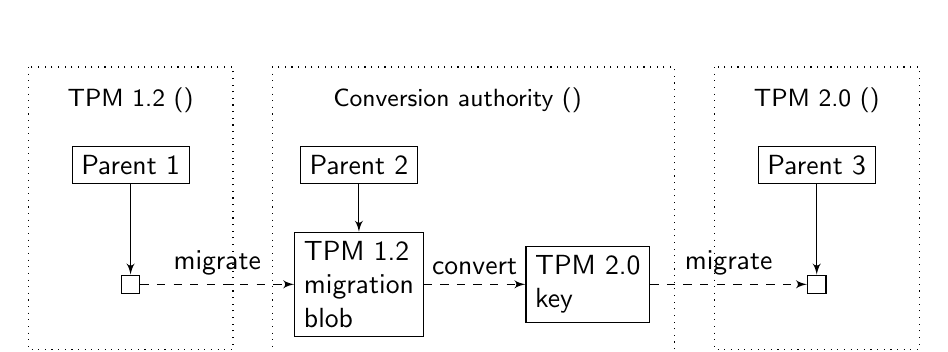
\begin{tikzpicture}[node distance=0.6cm,auto,>=latex',scale=1.0, every node/.style={scale=1.0}, font=\sffamily]
	% tpm 1.2 (tpms)
	\node[draw] (parent) at (0,0) {Parent 1};
	
	% % % % % % % %
	
	% conversion authority (tpmc)
	\node[draw,right=1.4cm of parent] (parentC) {Parent 2};
	%\node[draw,right=1.4cm of parentC] (parentC2) {Parent 3};
	\node[right=1.4cm of parentC,minimum width=1.5cm] (parentC2) {};
	
	\node[draw,below=of parentC,align=left] (tpm12migblob) {TPM 1.2\\migration\\blob};
	\node[draw,align=left] at (parentC2 |- tpm12migblob) (tpm20keyC) {TPM 2.0\\key};
	
	\draw[->] (parentC) to (tpm12migblob);
	%\draw[->] (parentC2) to (tpm20keyC);
	
	% box around all tpmc
	\node[above right=0.3cm and -1.2cm of parentC] {\small Conversion authority (\ca{})};
	\draw[dotted] ([xshift=-1.1cm,yshift=1cm]parentC.north) rectangle ([xshift=1.1cm,yshift=-.5cm]tpm20keyC.south);
		
	% % % % %
	% tpm 1.2 again
	
	\node[draw] at (parent |- tpm12migblob) (key) {\ek{}}; % use parent X and tpm12migblob Y coord.
	\draw[->] (parent) to (key);
	
	% box around all tpms
	\node[above=0.3cm of parent] {\small TPM 1.2 (\tpms{})};
	\draw[dotted] ([xshift=-1.3cm,yshift=1cm]parent.north) rectangle ([xshift=1.3cm,yshift=-0.7cm]key.south);
	
	% % % % % % %
	
	% tpm 2.0
	\node[draw,right=1.4cm of parentC2] (parent2) {Parent 3};
	\node[draw] at (parent2 |- tpm20keyC) (key2) {\ek{}};
	
	\draw[->] (parent2) to (key2);
	
	% box around all tpm 2.0
	\node[above=0.3cm of parent2] {\small TPM 2.0 (\tpmd{})};
	\draw[dotted] ([xshift=-1.3cm,yshift=1cm]parent2.north) rectangle ([xshift=1.3cm,yshift=-0.7cm]key2.south);
	
	% mapping between entities.
	\draw[->,dashed] (key.east) to node {migrate} (tpm12migblob.west);
	\draw[->,dashed] (tpm12migblob.east) to node {convert} (tpm20keyC.west);
	\draw[->,dashed] (tpm20keyC.east) to node {migrate} (key2.west);
	\end{tikzpicture}
	\caption{Overview of migration using the conversion authority}
	\label{fig:conversionoverview}
\end{figure}

\subsubsection{Conversion}
The conversion authority will perform the conversion of the key. The following are some important steps in this process.

TPM 2.0 supports a wide range of hash functions, and each key has a property \tpmc{nameAlg} which stores the algorithm for the key. We set \tpmc{nameAlg} of the TPM 2.0 key to be SHA-1, since that is the only supported hash algorithm in TPM 1.2. After this, the \tpmc{usageAuth} in the TPM 1.2 key (which is the SHA-1 hash of some secret) can be moved as-is to the TPM 2.0 formatted key.

Next, we want to move the public and private part of the source key. The public part of the key, which is simply a structure from the TPM 1.2 specification, must be sent separately to \ca{}, since it is not included in the migration blob. This contains the public modulus and exponent.

The private part of the key, which we obtained by manually decrypting the migration blob with the key of \ca{}, can be copied directly to the sensitive structure in TPM 2.0, since both TPM specifications states that the private part of RSA keys is one of the two RSA primes. % (TPM 1.2: part 2, rev 116, page 93, TPM 2.0: part 2, rev 01.16, page 134)

\subsubsection{Migration of the Migration Secret} \label{sec:migmigkeymigauth}
In TPM 1.2, each key has a migration secret, in addition to usage secret. If the value of this secret is \emph{tpmProof}, no migration is possible since \emph{tpmProof} is a value internal to the TPM. However, if the migration secret is the hash of a secret known to the user, migration is possible.

In TPM 2.0 there is no direct equivalent of the migration secret (which is called \tpmc{migrationAuth}) in TPM 1.2.
%An initial analysis give the following four options, of which only one fulfills our requirements.
An analysis of the migration secret functionality provides the following four options.

\begin{enumerate}
	\item Disallow any further migration, that is, once migrated to TPM 2.0, no more migrations will be possible. This violates requirement~\ref{req:furthermigration}.
	\item Always allow migration, that is, anyone can migrate the key. This violates requirement~\ref{req:migrationauth}.
	\item Only allow migration if the user knows the \tpmc{usageAuth}. This can be implemented through a simple policy. However, this violates requirement~\ref{req:migrationauth}.\label{itm:migrationsecretusage}
	\item Construct a more complex policy, which emulates the \tpmc{migrationAuth} behavior of TPM 1.2. \label{itm:migrationsecretmig}
\end{enumerate}

Of these options, option~\ref{itm:migrationsecretmig} is the only one which fulfills our requirements, and most closely resembles the original behavior of \tpms{}. Thus, when migrating \ek{} to \tpmd{}, we wish to keep the same migration secret, such that only entities with knowledge of the migration secret can migrate the key further.

In TPM 2.0, migration authorization is performed using policies. Thus, to keep the same migration secret, we must find a policy scheme that mimics the behavior of TPM 1.2.

An initial thought may be to utilize the commands \tpmct{PolicyAuthValue} or \tpmct{PolicyPassword} command in combination with setting the command code with \tpmct{PolicyCommandCode(TPM\_CC\_DUPLICATION)}, which would allow migration to any destination as long as a secret is known. However, both \tpmct{PolicyAuthValue} and \tpmct{PolicyPassword} use the \tpmc{authValue} of the key, which is the same secret which is required for regular usage of the key. This would correspond to our discarded option \ref{itm:migrationsecretusage} in the list above.

In the general case, the migration and usage secret will be different, and thus these two policy commands do not offer a solution to our problem. Another possibility is to use \tpmct{PolicySecret}. This policy command uses the \tpmc{authValue} of \emph{another} entity in the TPM. Thus we could imagine a scenario where a new, separate entity, whose only purpose is to keep the previous \tpmc{migrationAuth} as its own usage auth, is created. In this way, we could create a policy with the command \tpmct{PolicySecret} which uses this extra entity.

However, we have chosen another approach, which somewhat mimics the scenario where we have an MSA that approves our migration. This makes our proposed solution more consistent when we later on start considering CMKs. The proposed solution is depicted in \autoref{fig:migauthsibling}.

\begin{figure}[htbp]
	\centering
	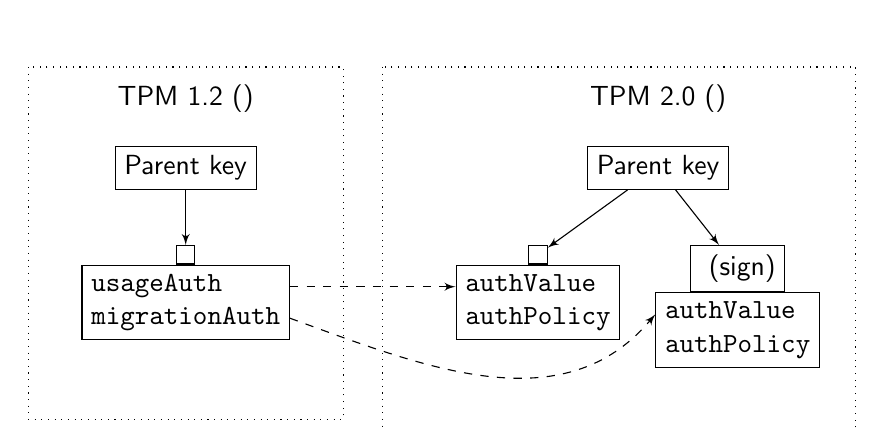
\begin{tikzpicture}[node distance=0.7cm,auto,>=latex',scale=1.0, every node/.style={scale=1.0}, font=\sffamily]
	\def\nd{0.7cm}
	% tpm 1.2
	\def\linedelta{0.20cm}
	\node[draw] (parent) at (0,0) {Parent key};
	
	\node[draw,below=of parent] (key) {\ek{}};
	\node[draw,below=0cm of key,align=left] (keysec) {\texttt{usageAuth}\\ \texttt{migrationAuth}};
	
	\draw[->] (parent) to (key);
	
	% box around all tpm 1.2
	\node[above=0.3cm of parent] {TPM 1.2 (\tpms{})};
	\draw[dotted] ([xshift=-2cm,yshift=1cm]parent.north) rectangle ([xshift=2cm,yshift=-1cm]keysec.south);
	
	% tpm 2.0
	\node[draw] (parent2) at (6,0) {Parent key};
	
	\node[draw,below left=\nd and 0.5cm of parent2] (key2) {\ek{}};
	\node[draw,below=0cm of key2,align=left] (keysec2) {\texttt{authValue}\\ \texttt{authPolicy}};
	
	\node[draw,below right=\nd and -0.5cm of parent2] (key2sibling) {\eksib{} (sign)};
	\node[draw,below=0cm of key2sibling,align=left] (keysec2sibling) {\texttt{authValue}\\ \texttt{authPolicy}};
	
	\draw[->] (parent2) to (key2);
	\draw[->] (parent2) to (key2sibling);
	
	% box around all tpm 2.0
	\node[above=0.3cm of parent2] {TPM 2.0 (\tpmd{})};
	\draw[dotted] ([xshift=-3.5cm,yshift=1cm]parent2.north) rectangle ([xshift=1.5cm,yshift=-0.9cm]keysec2sibling.south);
	
	% mapping between 1.2 and 2.0
	\draw[->,dashed] ([yshift=\linedelta]keysec.east) to ([yshift=\linedelta]keysec2.west);
	\draw[->,dashed] ([yshift=-\linedelta]keysec.east) to [out=-20,in=230] ([yshift=\linedelta]keysec2sibling.west);
	\end{tikzpicture}
	\caption{Migration secret in TPM 2.0}
	\label{fig:migauthsibling}
\end{figure}

The \tpmc{usageAuth} from our TPM 1.2 key is copied directly to the \tpmc{authValue} field of the TPM 2.0 key. We also copy the \tpmc{migrationAuth} from the TPM 1.2 key to the \texttt{authValue} field of a separate, newly created, signing key, called the \emph{sibling} key (\eksib{}), on the TPM 2.0. Thus, to be able to create signatures using the sibling key, we must know the \tpmc{authValue} of this key (which is the original \tpmc{migrationAuth}).

To control the migration of the key, we include a policy in the \tpmc{authPolicy} field of the key \ek{} at the destination TPM. We construct the policy such that a signature from the sibling key is required for a migration to succeed. To construct such a signature, the user clearly must have knowledge of the migration secret.

Constructing a policy which validates a signature can be done by using the policy command \tpmct{PolicySigned}. The policy will require the TPM user to present a signature from the sibling key (thus proving possession of the migration secret), and if valid,  \tpmct{PolicyCommandCode(TPM\_CC\_Duplicate)} is used to authorize a migration to any destination, mimicking the behavior of TPM 1.2.

Furthermore, in the \tpmc{authPolicy} field of the \emph{sibling key} we include a policy which allows migration of the sibling key as long as the \tpmc{authValue} is known. This allows us to migrate both the sibling key and \ek{} to another TPM 2.0 destination, which fulfills requirement~\ref{req:furthermigration}.

When creating \eksib{}, care must be taken to ensure that we get a deterministic creation. Simply creating a new, random, RSA keypair would violate requirement~\ref{req:deterministic}, since every migration of \ek{} would result in different \eksib{}, and thus different \tpmc{authPolicy} in \ek{}. Instead, we must base the generation of \eksib{} on \ek{}, to ensure that the generation is deterministic, yet unique for all keys. Assuming that the original private part of \ek{}, the pair of primes $(p,q)$, is random, we use a hash of $(p,q)$ as the seed to the prime number generator to construct new primes for the sibling key. This is similar to how TPM 2.0 generates primary objects (such as the SRK) using the primary seeds in the TPM. The process is depicted in \autoref{fig:pqtosibpq}.
%
Since we assumed that the original $(p,q)$ were random primes, our derived seed can also be considered random, thus giving a deterministic, but still secure \eksib{}. Clearly, if someone has knowledge of $(p,q)$ of \ek{}, they would be able to derive \eksib{}, and authorize a migration. However, if $(p,q)$ of \ek{} is already known, there is no reason for an attacker to do a migration, since the private part of \ek{} is already compromised.

\begin{figure}[tbp]
	\centering
	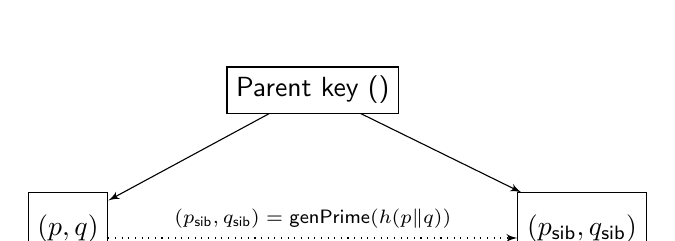
\begin{tikzpicture}[node distance=1cm,auto,>=latex',scale=1.0, every node/.style={scale=1.0}, font=\sffamily]

	% tpm 2.0
	\node[draw] (parent2) at (6,0) {Parent key (\tpmd{})};
	
	\node[draw,below left=1cm and 1.5cm of parent2,align=center] (key2) {\ek{} \\ $(p,q)$};
	
	\node[draw,below right=1cm and 1.5cm of parent2,align=center] (key2sibling) {\eksib{} \\ $(p_{\text{sib}},q_{\text{sib}})$};
	
	\draw[->] (parent2) to (key2);
	\draw[->] (parent2) to (key2sibling);
	
	\draw[->,dotted] ([yshift=-0.2cm]key2.east) to node {\scriptsize $(p_{\text{sib}},q_{\text{sib}}) = \text{genPrime}(h(p\|q))$} ([yshift=-0.2cm]key2sibling.west);
	% 
	% box around all tpm 2.0
	%\node[above=0.3cm of parent2] {TPM 2.0 (\tpmd{})};
	%\draw[dotted] ([xshift=-3.5cm,yshift=1cm]parent2.north) rectangle ([xshift=1.5cm,yshift=-1cm]keysec2sibling.south);
	\end{tikzpicture}
	\caption{Generating the primes for \eksib{} based on $(p,q)$ of \ek{}}
	\label{fig:pqtosibpq}
\end{figure}

\subsubsection{Owner Secret}
In TPM 1.2 the TPM owner is also required to authorize the migration. However this is not the case in TPM 2.0. We propose a solution where an extra signing key is introduced, similar to the sibling key above. However, different from the owner secret, this key is not unique per TPM, but rather per key. In a sense, it becomes an extra migration secret. It does deviate slightly from the behavior in TPM 1.2 since this owner signing key will have to be identical on all TPM 2.0 chips. The secret of the owner signing key is selected during the initial 1.2 to 2.0 migration, and the key will be created by the conversion authority. Just like for the migration key, the actual verification of the signature is done by including a \tpmct{PolicySigned} in the policy chain.

\subsection{PCR Bound Keys} \label{sec:pcrboundkeys}

In TPM 1.2, key usage can be restricted such that both certain PCR values (through \texttt{pcrSelection}) and knowledge of the \texttt{usageAuth} is required. In TPM 2.0, this must be implemented through the use of policies. As can be seen in \cite[Part 1, Annex A]{TPM2.0r16}, this can be realized by combining the use of \tpmct{PolicyPCR} and \tpmct{PolicyAuthValue}. When converting the key to TPM 2.0-format, it is important to set the \tpmc{userWithAuth}-attribute to CLEAR, since otherwise the user could circumvent the PCR requirement by only providing the \tpmc{authValue}.

When migrating and converting from 1.2 to 2.0, the PCR values need to be moved from the \texttt{pcrSelection} structure and instead be included as a part of the \tpmct{PolicyPCR} policy.

However, it is not possible for \ca{} to extract the PCR values from the TPM 1.2 migration blob. This is because the TPM 1.2 PCR structure present in the TPM 1.2 key only contains the hash over a structure containing multiple PCR values. The exact steps to calculate this hash is described in \cite[Part 2, Sec. 5.4.1]{TPM1.2spec}.

To be able to convert the PCR values to a format suitable for TPM 2.0, we would require access to each individual PCR value. In TPM 2.0 we will use the hash of the concatenation of all PCR values
%(section 17.5 tpm 2.0 spec part 1)
in the \tpmct{PolicyPCR} command, which is not the same structure that were used in TPM 1.2.

Thus, since we cannot extract each individual PCR value from the composite hash of the key in TPM 1.2, we cannot reconstruct a TPM 2.0 key bound to the exact same PCR values, at least not given only a migration blob.
Therefore, the PCR values from \tpms{} must be provided separately to the \ca{} during the conversion step.

A migration using \tpmco{CreateMigrationBlob} does not require that the PCR values of the TPM are in the expected state. This means that we cannot be sure that reading PCR values using \tpmco{PCRRead} returns the PCR values required to use the key. Instead, this must be verified by the conversion authority. Assuming that the PCR values, and the corresponding PCR index, are sent to the conversion authority, it can verify that these are indeed the correct values by calculating the hash in the same way as the TPM 1.2, and then compare it to the hash in the migration blob. If they match, \ca{} can then use the PCR values when converting the key for TPM 2.0.

Assuming the correct PCR values are sent to the conversion authority, we can construct a policy using \tpmct{PolicyPCR} followed by \tpmct{PolicyAuthValue}, which when combined will require both the correct PCR values and the correct usage secret.

However, we must also combine this with the policy for migration authorization in \autoref{sec:migmigkeymigauth}, such that we both can have PCR requirements and migration requirements. This does not mean that a migration requires correct PCR values (this is not required in TPM 1.2 either), but that one of the two policy branches is satisfied.

Thus, we create a policy with two branches, combined with \tpmct{PolicyOR}, as in \autoref{fig:policypcror}. Either of the two branches can be satisfied, if the left branch is satisfied, key usage is granted (if the PCR values are correct). If the right branch is satisfied, migration is authorized.

\begin{figure}[htbp]
	\centering
%	\begin{tikzpicture}[node distance=0.3cm,auto,>=latex',scale=\policychainscalefactor, every node/.style={scale=\policychainscalefactor}]
%%	\node (pcr) at (0,0) {\tpmct{PolicyPCR}};
%%	\node[below=of pcr] (authvalue) {\tpmct{PolicyAuthValue}};
%%	
%%	\node[right=of pcr] (dupselect) {\tpmct{PolicyDuplicationSelect}};
%%	\node[below=of dupselect] (authorize) {\tpmct{PolicyAuthorize}};
%%	
%%	\node[below right=of authvalue] (or) {\tpmct{PolicyOR}};
%%	
%%	\draw[->] (pcr) to (authvalue);
%%	\draw[->] (authvalue) to (or);
%	
%	\matrix (m) [matrix of nodes, row sep=1.5em]
%	{ \tpmct{PolicyPCR} & & \tpmct{PolicySigned} \\
%	  \tpmct{PolicyAuthValue} & {} & \tpmct{PolicyCommandCode} \\  
%	};
%	\node[below=1.5em of m-2-2] (m-3-2) {\tpmct{PolicyOR}};
%	
%	\draw[->] (m-1-1) to (m-2-1);
%	\draw[->] (m-2-1) to (m-3-2);
%	
%	\draw[->] (m-1-3) to (m-2-3);
%	\draw[->] (m-2-3) to (m-3-2);
%	
%	\end{tikzpicture}
	
		\begin{tikzpicture}[node distance=0.3cm,auto,>=latex',scale=\policychainscalefactor, every node/.style={scale=\policychainscalefactor}]
		\matrix (m) [matrix of nodes, row sep=0.3cm]
		{
			&                  & \tpmct{PolicySigned} \\
			\tpmct{PolicyPCR}       &                  & \tpmct{PolicySigned} \\
			\tpmct{PolicyAuthValue} &                  & \tpmct{PolicyCommandCode} \\
			&                  & \\
		};
		\path (m-3-1) -- (m-3-3) node[midway] (m-3-2) {}; % helper node for placing the node below.
		\node[below=0.5cm of m-3-2] (m-4-2) {\tpmct{PolicyOR}};
		
		\draw[->] (m-2-1) to (m-3-1);
		\draw[->] (m-3-1) to (m-4-2);
		
		\draw[->] (m-1-3) to (m-2-3);
		\draw[->] (m-2-3) to (m-3-3);
		\draw[->] (m-3-3) to (m-4-2);
		\end{tikzpicture}
	\caption{Policy for PCR combined with migration authorization}
	\label{fig:policypcror}
\end{figure}

\subsection{Key Hierarchies} \label{sec:keyhierarchies}
Up until now, we have only considered the case where \ek{} is either a signing or a decryption key. If \ek{} is a storage key with child keys, we must be able to migrate the complete hierarchy as well.

Normally, when migrating keys either from 1.2 to 1.2, or from 2.0 to 2.0, there is no need to explicitly migrate the child keys. If the parent key is migrated and thus available in the destination TPM, all child keys can simply be loaded directly with \tpmco{LoadKey2} or \tpmct{Load}, using the same encrypted private part on both the source and destination, without any migration.

However, due to the difference in encryption and overall key storage format between 1.2 and 2.0, a more elaborate scheme is required when migrating a hierarchy from 1.2 to 2.0.

Recall that in TPM 1.2, the parent's public key is used to encrypt the child key's private part. Thus, asymmetric encryption is used. However, in TPM 2.0, symmetric encryption is used instead. The child key's private part is encrypted using a symmetric key derived from a \emph{seed} in the parent key. Normally, this seed is generated upon key creation, and is based on data from the RNG in the TPM. However, due to requirement~\ref{req:deterministic}, we require a deterministic seed.
%Otherwise, different subsequent migrations would yield different seeds, which would make it impossible to decrypt child keys stemming from another migration.
Otherwise, subsequent migrations of the same hierarchy would yield different seeds, and child keys would be encrypted with different symmetric keys, even though they share the same parent.

When migrating a complete key hierarchy, we introduce extra requirements on our solution:
\begin{enumerate}
	\item When migrating a hierarchy, only the migration secret of the hierarchy's root key should be required to migrate the root and all of its descendant keys.
	\item It should be possible to migrate parts of a hierarchy at different occasions.
\end{enumerate}

Assume the hierarchy of keys given in \autoref{fig:mighierarchy}. If we want to migrate \ek{}, including its child keys C1 and C2, we first perform a migration of \ek{} as usual, i.e. just like if it was a signature or decryption key. However, \ca{} can see that \ek{} is a storage key, and if this is the case we include a seed inside the TPM 2.0-version of the key.

\begin{figure}
	\centering
	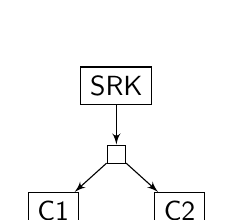
\begin{tikzpicture}[node distance=0.5cm,auto,>=latex',scale=1, every node/.style={scale=1}, font=\sffamily]
	\node[draw] (parent) at (0,0) {SRK};
	
	\node[draw,below=of parent] (key) {\ek{}};
	\node[draw,below left=of key] (keyc1) {C1};
	\node[draw,below right=of key] (keyc2) {C2};
	
	\draw[->] (parent) to (key);
	\draw[->] (key) to (keyc1);
	\draw[->] (key) to (keyc2);
	\end{tikzpicture}
	\caption{Key hierarchy}
	\label{fig:mighierarchy}
\end{figure}

We calculate the seed as $seed = \text{SHA1}(p \| q)$. The reason for using SHA-1 is because the seed must be of the same size as the \tpmc{nameAlg} of the key, which is set to SHA-1 to be able to use the same \tpmc{usageAuth} as in TPM 1.2.

When migrating a hierarchy, we also provide \ca{} with the encrypted private parts of the child keys of \ek{}, which we wish to migrate to \tpmd{}. When \ca{} receives this bundle of keys, it can use the private parts of \ek{} to decrypt all the other encrypted private parts of the child keys. The child keys can then be converted to TPM 2.0-format, and re-encrypted using the symmetric key derived from the seed.

This approach will work for hierarchies of any depth. However, the hierarchy must be preserved inside the bundle, since \ca{} must have access to the parent of a child key to be able to decrypt it. We can also migrate only parts of a deep hierarchy, as long as all relevant parents leading to \ek{} are included.

When migrating keys in the hierarchy, their migration secret must be preserved just as before. This means that in addition to converted child keys, we will also get sibling keys for each converted child key.
%
The sibling keys are placed so that they share parent with the key that they correspond to, see \autoref{fig:mighierarchysiblings}.

\begin{figure}
	\centering
	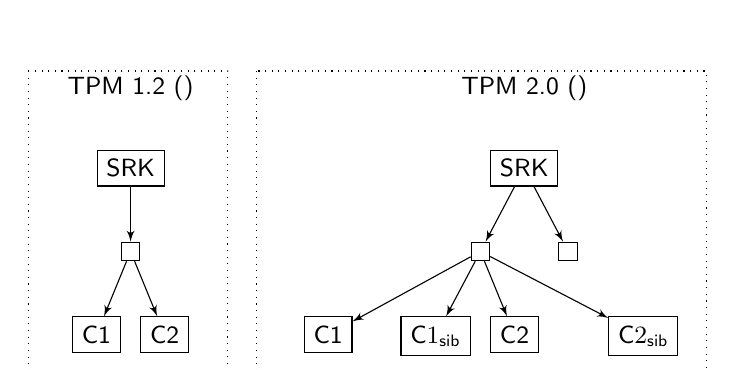
\begin{tikzpicture}[node distance=0.7cm,auto,>=latex',scale=1, every node/.style={scale=1}, font=\small\sffamily]
	\def\nd{0.7cm} % would be neat if node distance already had a command?
	% tpm 1.2
	\node[draw] (parent) at (0,0) {SRK};
	
	\node[draw,below=of parent] (key) {\ek{}};
	\node[draw,below left=\nd and 0cm of key] (keyc1) {C1};
	\node[draw,below right=\nd and 0cm of key] (keyc2) {C2};
	
	\draw[->] (parent) to (key);
	\draw[->] (key) to (keyc1);
	\draw[->] (key) to (keyc2);
	
	% box around all tpm 1.2
	\node[above=0.5cm of parent] {TPM 1.2 (\tpms{})};
	\draw[dotted] ([xshift=-1.3cm,yshift=1cm]parent.north) rectangle ([xshift=0.8cm,yshift=-0.3cm]keyc2.south);
	
	% tpm 2.0
	\node[draw] (parent2) at (5,0) {SRK};
	
	\node[draw,below left=\nd and 0.0cm of parent2] (key2) {\ek{}};
	\node[draw,below right=\nd and 0.0cm of parent2] (key2sibling) {\eksib{}};
	
	\node[draw,below left=\nd and 1.5cm of key2] (key2c1) {C1};
	\node[draw,below left=\nd and 0cm of key2] (key2c1sibling) {C$1_\text{sib}$};
	
	\node[draw,below right=\nd and 0cm of key2] (key2c2) {C2};
	\node[draw,below right=\nd and 1.5cm of key2] (key2c2sibling) {C$2_\text{sib}$};
	
	\draw[->] (parent2) to (key2);
	\draw[->] (parent2) to (key2sibling);
	\draw[->] (key2) to (key2c1);
	\draw[->] (key2) to (key2c1sibling);
	\draw[->] (key2) to (key2c2);
	\draw[->] (key2) to (key2c2sibling);
	
	% box around all tpm 2.0
	\node[above=0.5cm of parent2] {TPM 2.0 (\tpmd{})};
	\draw[dotted] ([xshift=-3.4cm,yshift=1cm]parent2.north) rectangle ([xshift=0.8cm,yshift=-0.3cm]key2c2sibling.south);
	
	% mapping between 1.2 and 2.0

	\end{tikzpicture}
	\caption{Key hierarchy and sibling keys}
	\label{fig:mighierarchysiblings}
\end{figure}

\section{Certifiable Migratable Keys} \label{sec:cmks}
In TPM 1.2, a CMK can only be migrated with the approval of both the TPM owner and a third-party Migration Selection Authority (MSA).

In TPM 2.0, there is no direct equivalent of CMK, but the behavior can be achieved by using policies as in \autoref{fig:policycmk}. \tpmct{PolicyAuthorize} allows us to replace the previous commands in the policy chain, in this case, it allows us to replace \tpmct{PolicyDuplicationSelect} with another destination, as long as we can present a valid signature of the policy hash. This signature is done by the authority (MSA in TPM 1.2 terminology).

In this way the MSA must approve the destination before any migration can be performed, and the approval is only valid for a specific destination.

\begin{figure}[htbp]
	\centering
	\begin{tikzpicture}[node distance=0.3cm,auto,>=latex',scale=\policychainscalefactor, every node/.style={scale=\policychainscalefactor}]
		\node (dupselect) at (0,0) {\tpmct{PolicyDuplicationSelect}};
		\node[below=of dupselect] (authorize) {\tpmct{PolicyAuthorize}};
		
		\draw[->] (dupselect) to (authorize);
	\end{tikzpicture}
	\caption{Policy for CMK}
	\label{fig:policycmk}
\end{figure}

A complication introduced by CMKs is that TPM 1.2 introduces restrictions on the place of CMKs in the key hierarchy. A CMK cannot be the child of a migratable key, nor can it be the child of another CMK. When we convert a CMK into TPM 2.0 format, we must ensure that these restrictions still hold. Otherwise we would violate requirement~\ref{req:migrationauth}, since we would be able to further migrate the child CMK if we were authorized to migrate the migratable parent.

Thus, when migrating a CMK, we must ensure that the destination parent is not a migratable key. This is the responsibility of the MSA, and is not discussed any further.

We consider the three cases in the previous section, and construct the required policy for each case.

\subsection{Signing or Decryption Key} \label{sec:cmksimple}
When using CMKs, there is no migration secret that the key owner needs to present. In \autoref{sec:simple} we presented a solution where two \tpmct{PolicySigned} commands were included in the \tpmc{authPolicy} of \ek{}. In the CMK case, we can remove one of the signatures, since there is no migration secret. This also means that no sibling key is required, we can consider the key of the MSA as our (remote) sibling key.

Since there is no built-in requirement in TPM 2.0 for the owner to authorize a migration, we introduced an owner signing key. This signature is still required in the CMK case. 

We can do this by simply adding the \tpmct{PolicySigned} command to the end of the chain. Note that adding it to the start of the chain would make it possible for the authority to override the owner authorization, which we want to avoid. Thus the chain now look like in \autoref{fig:policycmkmig}. \tpmct{PolicyDuplicationSelect} will set the command code to \tpmc{TPM\_CC\_Duplicate}, so no explicit call to set the command code is required after \tpmct{PolicySigned}.
\begin{figure}[bhtp]
	\centering
	\begin{tikzpicture}[node distance=0.3cm,auto,>=latex',scale=\policychainscalefactor, every node/.style={scale=\policychainscalefactor}]
	\node (dupselect) at (0,0) {\tpmct{PolicyDuplicationSelect}};
	\node[below=of dupselect] (authorize) {\tpmct{PolicyAuthorize}};
	\node[below=of authorize] (signed) {\tpmct{PolicySigned}};
	
	\draw[->] (dupselect) to (authorize);
	\draw[->] (authorize) to (signed);
	\end{tikzpicture}
	\caption{Policy for CMK, with owner authorization}
	\label{fig:policycmkmig}
\end{figure}

\subsection{PCR Bound Keys}
We start with the policy from the previous section, and add a PCR policy, similar to what we did in \autoref{sec:pcrboundkeys}. Again, we get two different branches of the policy, one for usage, and one for migration, see \autoref{fig:policycmkpcror}. Just like before, either of the two branches can be satisfied. If the left branch is satisfied, key usage is granted (if the PCR values are correct). If the right branch is satisfied, migration is authorized, because \tpmct{PolicyDuplicationSelect} will set the correct command code for migration.

\begin{figure}[htbp]
	\centering
	\begin{tikzpicture}[node distance=0.3cm,auto,>=latex',scale=\policychainscalefactor, every node/.style={scale=\policychainscalefactor}]
%		\matrix (m) [matrix of nodes, row sep=0.3cm]
%		{
%			                        &                  & \tpmct{PolicyDuplicationSelect} \\
%			\tpmct{PolicyPCR}       &                  & \tpmct{PolicyAuthorize} \\
%			\tpmct{PolicyAuthValue} &                  & \tpmct{PolicySigned} \\
%			                        & \tpmct{PolicyOR} & \\
%		};
%		
%		\draw[->] (m-2-1) to (m-3-1);
%		\draw[->] (m-3-1) to (m-4-2);
%		
%		\draw[->] (m-1-3) to (m-2-3);
%		\draw[->] (m-2-3) to (m-3-3);
%		\draw[->] (m-3-3) to (m-4-2);
		\matrix (m) [matrix of nodes, row sep=0.3cm]
		{
			                        &                  & \tpmct{PolicyDuplicationSelect} \\
			\tpmct{PolicyPCR}       &                  & \tpmct{PolicyAuthorize} \\
			\tpmct{PolicyAuthValue} &                  & \tpmct{PolicySigned} \\
			                        &                  & \\
		};
		\path (m-3-1) -- (m-3-3) node[midway] (m-3-2) {}; % helper node for placing the node below.
		\node[below=0.5cm of m-3-2] (m-4-2) {\tpmct{PolicyOR}};
		
		\draw[->] (m-2-1) to (m-3-1);
		\draw[->] (m-3-1) to (m-4-2);
		
		\draw[->] (m-1-3) to (m-2-3);
		\draw[->] (m-2-3) to (m-3-3);
		\draw[->] (m-3-3) to (m-4-2);
		\end{tikzpicture}
	\caption{Policy for PCR combined with migration authorization and CMK}
	\label{fig:policycmkpcror}
\end{figure}

\subsection{Storage Keys}
Recall the restrictions on CMKs in the key hierarchy. A CMK may not have a migratable parent, neither a regular migratable key nor a CMK. The effect is the only possible key hierarchy which includes CMKs is a hierarchy where the root node is a CMK. This means that we can proceed as in \autoref{sec:keyhierarchies}, with the additional requirement that the root CMK key gets a policy just like in \autoref{sec:cmksimple}.

\section{Implementation} \label{sec:tpm12to20:implementation}
To ensure that our conversion process works as intended, we have implemented all the above test cases, and verified their behavior. The TPMs have been emulated in software. For TPM 1.2, IBM's Software TPM version 4720 \cite{ibmswtpm} has been used. For TPM 2.0, Microsoft's TPM2 Simulator version 1.1 \cite{mstpm2sim} has been used.

To simplify the implementation, we have assumed the following:

\begin{itemize}
	\item All TPM 1.2 keys are in the \texttt{TPM\_KEY12}-key format.
	\item \ek{} is 2048 bit RSA, two primes. Two primes and RSA is a requirement for migratable keys according to \cite[Part 2, Sec. 10.7]{TPM1.2spec}. %[TPM 1.2 spec part 2 sec. 10.7 p. 93].
	\item The default RSA exponent ($2^{16}+1$) is used for all keys. For storage keys this is also required by the TPM 1.2 specification. %(TPM 1.2 spec part 3 sec 10.4)).
\end{itemize}

The TPM 1.2 specification in \cite{TPM1.2spec} has no defined formats on how to send migration packages between the different entities. It does, however, exist a specification \cite{TPMmigrationservices-tcg} which describes an XML schema for supplying information about keys during the migration phase. This specification is, however, not fully updated for TPM 1.2, but rather based on TPM 1.1, and thus we have not used this XML-based approach in our implementation.

Instead, since our implementation was primary meant for testing and evaluation purposes, we have simply passed files with binary content between the different entities.

\section{Related Work} \label{sec:tpm12to20:relatedwork}
While there are few widespread applications that rely on the functionality provided by the TPM, there are examples of existing pieces of software, and some other proposed use cases. From Microsoft we have both Bitlocker \cite{Bitlocker}, used for full-disk encryption, and Virtual Smart Cards \cite{microsoft-vsc}, which uses the TPM instead of physical smart cards to store private keys.
Examples of proposed use cases for the newer TPM 2.0 are for example the use of TPM for tamper-proof logging \cite{sinha:2014}, or the use of TPM 2.0 for electronic identities \cite{nyman:2014}.

Related to the challenge of providing consistent behavior between the two TPM versions, in \cite{hell:2014}, the authors design a unified API which implements their functionality on both TPM 1.2 and 2.0. In contrast to this work, they consider the functionality for a certain use case, and then create two different and separate implementations, one for each TPM version, with no possibility of key migration between them.

The use of TPMs to provide trusted computing functionality within cloud computing is an area where there also has been development and research. In \cite{santos:2009} the use of trusted computing in cloud platforms is discussed, and in \cite{srivastava:2012} trusted snapshots of running virtual machines is discussed. Related to migrating keys between TPMs are ways of sharing keys between different TPMs. A cloud-based solution is proposed in \cite{chen:2014}.

\section{Conclusions} \label{sec:discussion}
We have proposed a solution to make it possible to move or copy key material from TPM 1.2 to TPM 2.0. Even though the two TPM versions differ significantly in functionality, and offer no backward compatibility, we have presented a design which allows the migration of keys between different versions, while still maintaining the same functionality.
This allows users of the current TPM 1.2 version to start using the newer TPM 2.0 chips, still keeping the same encryption keys and functionality. In this way, previously encrypted data can be decrypted with the same set of authorization requirements as before.
The required functionality was first identified and organized as a set of requirements. After this we looked at several different cases, where each case corresponded to different properties of the source key on the TPM 1.2.

We presented a way to provide the migration secret functionality of TPM 1.2 also in TPM 2.0. By introducing sibling keys and using policies, we can maintain the same authorization requirements in both TPM versions.
We also handle migration of PCR bound keys from TPM 1.2 to TPM 2.0. Because of the differences in key format between the two versions, the migration requires PCR values to be sent to the conversion authority. The conversion authority can then verify the values against the source key before including them in the destination key.
In addition to this, we showed how the TPM 1.2 CMK functionality can be expressed in terms of TPM 2.0 policies, and combined this with the previous results so that migration of all key types of TPM 1.2 are covered.
%For each case, we proposed a solution which maintained the properties of the source key after it has been moved to the TPM 2.0 domain. This was mainly done by utilizing policies in TPM 2.0.
Finally the different proposed solutions were implemented and tested using TPM emulators.

\subsubsection{Acknowledgments.}The authors would like to thank the anonymous reviewers for their helpful and valuable comments.


%\bibliographystyle{IEEEtran}
%\bibliographystyle{splncs03}

%\bibliography{tpm12to20}
% Generated by the bibfile above.


{\raggedright
	\printbibliography[segment=\therefsegment,heading=subbibliography]
}

}

%\begin{thebibliography}{10}
%\providecommand{\url}[1]{\texttt{#1}}
%\providecommand{\urlprefix}{URL }
%
%\bibitem{chen+raj-ctpm:14}
%Chen, C., Raj, H., Saroiu, S., Wolman, A.: {cTPM: A Cloud TPM for Cross-Device
%  Trusted Applications}. In: 11th USENIX Symposium on Networked Systems Design
%  and Implementation (NSDI 14). USENIX Association, Seattle, WA (Apr 2014)
%
%\bibitem{hell+karlsson-tpmsecurestorage:14}
%Hell, M., Karlsson, L., Smeets, B., Mirosavljevic, J.: {Using TPM Secure
%  Storage in Trusted High Availability Systems}. In: {Trusted Systems: 6th
%  International Conference, INTRUST 2014, Beijing, China}. pp. 243--258.
%  Springer International Publishing (2015)
%
%\bibitem{ibmswtpm}
%IBM: {IBM}'s software trusted platform module.
%  \url{http://ibmswtpm.sourceforge.net/}
%
%\bibitem{infineon-tpm20-released}
%Infineon: {Infineon Advances Trusted Computing with New OPTIGA\texttrademark{}
%  TPM Family: Security Chips Serve Industrial/Embedded Environments and Support
%  Next Generation TPM 2.0 Firmware}.
%  \url{http://www.infineon.com/cms/en/about-infineon/press/press-releases/2013/INFCCS201309-062.html}
%
%\bibitem{infineon-tpm20-surfacepro}
%Infineon: {Infineon Expands its Trusted Computing Expertise to Mobile Devices:
%  OPTIGA\texttrademark{} TPM 2.0 Chips Secure Microsoft Surface Pro 3 Tablet}.
%  \url{http://www.infineon.com/cms/en/about-infineon/press/press-releases/2015/INFCCS201502-026.html}
%
%\bibitem{microsoft-bitlocker}
%Microsoft: {BitLocker Drive Encryption Overview}.
%  \url{https://www.microsoft.com/en-us/download/details.aspx?id=29076}
%
%\bibitem{mstpm2sim}
%Microsoft: {TSS.MSR} v1.1 {TPM2} simulator.
%  \url{http://research.microsoft.com/en-US/downloads/35116857-e544-4003-8e7b-584182dc6833/default.aspx}
%
%\bibitem{microsoft-vsc}
%{Microsoft}: {Understanding and Evaluating Virtual Smart Cards} (July 2014)
%
%\bibitem{Nyman:2014:CEI:2666141.2666146}
%Nyman, T., Ekberg, J.E., Asokan, N.: {Citizen Electronic Identities Using TPM
%  2.0}. In: Proceedings of the 4th International Workshop on Trustworthy
%  Embedded Devices. pp. 37--48. TrustED '14, ACM, New York, NY, USA (2014)
%
%\bibitem{santos+gummadi+rodrigues-towardstcc:09}
%Santos, N., Gummadi, K.P., Rodrigues, R.: Towards trusted cloud computing. In:
%  Proceedings of the 2009 conference on Hot topics in cloud computing. USENIX
%  Association (2009)
%
%\bibitem{sinha+jia-tamperprooflogging:14}
%Sinha, A., Jia, L., England, P., Lorch, J.R.: {Continuous Tamper-Proof Logging
%  Using TPM 2.0}. In: {Trust and Trustworthy Computing: 7th International
%  Conference, TRUST 2014}. pp. 19--36. Springer International Publishing (2014)
%
%\bibitem{Srivastava-trustedvmsnapshots:12}
%Srivastava, A., Raj, H., Giffin, J., England, P.: Trusted VM Snapshots in
%  Untrusted Cloud Infrastructures, pp. 1--21. Springer Berlin Heidelberg,
%  Berlin, Heidelberg (2012)
%
%\bibitem{TPM1.1bspec-tcg}
%{Trusted Computing Group}: {Trusted Computing Platform Alliance (TCPA) Main
%  Specification Version 1.1b} (February 2002)
%
%\bibitem{TPMmigrationservices-tcg}
%{Trusted Computing Group}: {Interoperability Specification for Backup and
%  Migration Services, Specification Version: 1.0 Final, Revision 1.0 } (June
%  2005)
%
%\bibitem{TPM1.2spec-tcg}
%{Trusted Computing Group}: {TPM} main specification, Version 1.2, Revision 116
%  (March 2011)
%
%\bibitem{TPM2.0spec-tcg}
%{Trusted Computing Group}: Trusted Platform Module Library Specification,
%  Family "2.0", Level 00, Revision 01.16 (October 2014)
%
%\end{thebibliography}


\fi

\ifpaperIII
\newrefsegment
\addtolength{\apa}{2cm}
\fancyhead[RE]{\paperref{ch:trustanchors}: \paperIIItitle}
\chapter[\paperIIItitle]{\texorpdfstring{%
		Trust Anchors in\\Software Defined Networks}{%
		\paperIIItitle}}
\label{ch:trustanchors}
\paperRemark{\paperIIIref}

{

%\documentclass{llncs}
%\usepackage[utf8]{inputenc}
%\usepackage{amsmath}
%\usepackage{amsfonts}
%\usepackage{amssymb}
%\usepackage{booktabs}
%\usepackage{makecell}
%\usepackage{multirow}
%\usepackage{soul}
%\usepackage{tikz}
%\usepackage{todonotes}
%
%\usepackage[hidelinks]{hyperref}
%\renewcommand\UrlFont{\color{blue}\rmfamily}

\newcommand*\circled[1]{\tikz[baseline=(char.base)]{
            \node[shape=circle,draw,inner sep=1pt, color=white,fill=black] (char) {#1};}}





%\begin{document}
%
%\title{Trust Anchors in Software Defined Networks}	
%
%\author{Nicolae Paladi\inst{1} \and
%Linus Karlsson\inst{2} \and
%Khalid Elbashir\inst{3}}
%
%\institute{RISE SICS \\ \email{nicolae.paladi@ri.se} \and
%Lund University \\ \email{linus.karlsson@eit.lth.se} \and
%KTH - Royal Institute of Technology \\ \email{elbashir@kth.se}}
%
%\maketitle

\section*{Abstract}
Advances in software virtualization and network processing lead to increasing network softwarization.
Software network elements running on commodity platforms replace or complement hardware components in cloud and mobile network infrastructure.
However, such commodity platforms have a large attack surface and often lack granular control and tight integration of the underlying hardware and software stack.
Often, software network elements are either themselves vulnerable to software attacks or can be compromised through the bloated trusted computing base.
To address this, we protect the core security assets of network elements -- authentication credentials and cryptographic context -- by provisioning them to and maintaining them exclusively in isolated execution environments.
We complement this with a secure and scalable mechanism to enroll network elements into software defined networks.
Our evaluation results show a negligible impact on run-time performance and only a moderate performance impact at the deployment stage.

%=====================================================================================
\section{Introduction}
\label{sec:intro}
%=====================================================================================
Software Defined Networking (SDN) is a widely used approach to operate network infrastructure in virtualized environments.
Separation of forwarding and control logic, a core idea of this model, is often realized by software network elements in a virtualized network infrastructure deployed on commodity hardware.
However, by departing from hardware network elements with tightly couped software and hardware often provided by the same vendor~\cite{etsinfv:2013},
SDN broke previous assumptions, outdated best-practices and introduced new vulnerabilities~\cite{paladi:2015,paladi:2017c}.
Scott-Hayward et al. outlined a series of attack vectors that can lead to unauthorized access, data leakage or modification, malicious applications on the network, configuration issues, and a wider collection of system-level security vulnerabilities~\cite{scott:2015}.
This concern applies to both the data plane and the application plane in SDN deployments.
On the data plane, related literature describes both potential attacks on SDN in case of a virtual switch compromise~\cite{antikainen:2014}, partly demonstrated in~\cite{thimmaraju:2017}.
Malicious applications deployed on the SDN infrastructure are a particular concern in virtualized environments. 
They affect network security both directly (by intercepting or modifying traffic), or indirectly through horizontal attacks aimed to leak authentication credentials and encryption keys~\cite{itu-t:2016}.

Earlier research addressed SDN security through additional services~\cite{porras:2012,shin:2013,hu:2014}, formal verification~\cite{ball:2014} and isolated execution using Intel Software Guard Extensions (SGX)~\cite{shih:2016,paladi:2016b,kim:2017,paladi:2017b}, and most popular network element implementation support communication over transport layer security (TLS)~\cite{rfc5246}.
Despite these efforts, the confidentiality and integrity of authentication credentials of network elements in SDN remain unaddressed.
In particular, the existing approaches to provision authentication credentials to network elements in SDN are either plain insecure or both insecure and unscalable, requiring manual steps\footnote{Indeed, the Open vSwitch manual contains phrases as 
``Write the fingerprint down on a slip of paper and copy sc-req.pem to the machine that contains the PKI structure''}~\cite{ovs_ssl}.
Moreover, credentials provisioned to network elements in virtualized environments are often stored in plaintext on the file system.
Adversaries exploiting vulnerabilities in process and virtualization isolation can access authentication credentials to perform network attacks or impersonate network elements.
In this paper, we address two complementary questions:
(1) \textit{How can authentication credentials be securely provisioned to software network elements in SDN deployments?}
and 
(2) \textit{How can the TLS context of virtual switches be protected on compromised hosts?}

\subsection{Contributions}
\label{subsec:contrib}
In this work, we present the following contributions:
\begin{itemize}
	\item A secure, practical, and scalable mechanism to provision authentication credentials and bootstrap communication between software network elements.
	\item TLSonSGX\footnote{Source code available: \url{https://github.com/TLSonSGX/TLSonSGX}}, a library allowing to maintain authentication credentials and the TLS context exclusively in isolated execution environments. 
	\item A novel approach to restricting the availability of authentication credentials for SDN components to hosts with an attested trusted computing base.
	\item A first thorough analysis of the performance trade-offs of deploying components of network elements in SGX enclaves.
\end{itemize}

\subsection{Structure}
\label{subsec:structure}
The remainder of this paper is structured as follows.
We present the system model and threat model in~\S\ref{sec:sys-threat-mod}.
Next, we describe the proposed solution in~\S\ref{sec:arch} and its implementation in \S\ref{sec:implem}.
We evaluate the approach in~\S\ref{sec:eval}, discuss the related work in~\S\ref{sec:related-work}, outline limitations and future work in~\S\ref{sec:future_work} and conclude in~\S\ref{sec:trustanchors:conclusion}.

%=====================================================================================
\section{System and Threat Model}
\label{sec:sys-threat-mod}
%=====================================================================================
We consider an SDN infrastructure deployed on commodity platforms in a distributed system, such as in a cloud platform or a mobile communications network.
The infrastructure is managed by the \textit{administrators} of a \textit{network operator}.
Physical access to the platforms is restricted and auditable.

\paragraph{System model} 
Administrators use \textit{orchestrators} to manage network infrastructure, software components and network services~\cite{etsinfv:2013}.
They deploy network elements on the \textit{data plane}, \textit{control plane} and \textit{application plane}. % over a dedicated management network.
The \textit{data plane} consists of hardware or software switches (e.g. Open vSwitch~\cite{pfaff:2015}) and communication links between them.
The \textit{control plane} consists of a logically centralized \textit{network controller} (e.g. ONOS~\cite{berde:2014}, Floodlight~\cite{floodlightapi}).
The network controller manages software switches through protocols such as OpenFlow~\cite{mckeown:2008} (to add or remove flows) or OVSDB~\cite{rfc7047} (to create ports and tunnels); 
it manages hardware switches through OpenFlow (if supported) or other interfaces, such as NETCONF~\cite{rfc6241}.
The \textit{application plane} comprises \textit{network functions} that implement services such as traffic engineering, monitoring, or caching.
A \textit{Virtual Network Function} (VNF) is a virtualisation of a network function~\cite{etsinfv:2013}.
Orchestrators deploy VNFs upon request from the network controller or a tenant. 
The network controller configures flows and steers traffic to the network functions.

Network elements on the data-, control-, and application planes communicate over two application programming interfaces (APIs).
The controller communicates with data plane elements over the \textit{southbound} API, commonly Openflow~\cite{mckeown:2008,sherwood:2010,bifulco:2016} and with application plane elements over the \textit{northbound} API.

At deployment time, the orchestrator provisions TLS certificates to network elements during the \textit{enrollment} process.
Furthermore, to protect the data within the SDN deployment, the network controller enforces communication over TLS with mutual authentication on both southbound and northbound APIs.

\paragraph{Threat model} Similar to earlier work on SDN security threats \cite{kreutz:2013,paladi:2015}, we assume physical security of the platforms underlying the SDN infrastructure and correct implementation of cryptographic algorithms and communication security protocols, such as TLS~\cite{rfc5246}. 
The adversary has the capabilities of a system administrator with remote access to commodity platforms in the SDN infrastructure.
The adversary can intercept, drop and modify packets on the southbound and northbound interfaces.
Furthermore, the adversary can run arbitrary network elements in the SDN deployment and elsewhere~\cite{etsinfv:2013}. 
The adversary can read the memory of the commodity platforms, exploit vulnerabilities in network elements on the data- and application planes, and circumvent virtualization isolation~\cite{antikainen:2014}.

%=====================================================================================
\section{Solution Space}
\label{sec:arch}
%=====================================================================================
We next present the approach for provisioning and protecting authentication credentials on the data and application planes of SDN deployments.
We first introduce three building blocks to create trust anchors in SDN deployments: 
Software Guard Extensions (SGX), Trusted Platform Module (TPM) and Integrity Measurement Architecture (IMA).

%=====================================================================================
\subsection{Trust Anchors}
\label{subsec:trust-anchors}
%=====================================================================================
We use SGX enclaves~\cite{anati:2013,mckeen:2013,xing:2016,mckeen:2016} to create trusted execution environments (TEEs) during operating system execution.
We use the TEEs to store authentication credentials and execute cryptographic operations for network elements.
SGX enclaves rely on a trusted computing base (TCB) of code and data loaded at enclave creation time, processor firmware and processor hardware.
Program execution within an enclave is transparent to the underlying operating system and other mutually distrusting enclaves on the platform.
Enclaves operate in a dedicated memory area called the Enclave Page Cache, a range of DRAM that cannot be accessed by system software or peripherals~\cite{mckeen:2013,intel64}.
The CPU firmware and hardware are the root of trust of an enclave;
it prevents access to the enclave's memory by the operating system and other enclaves.
Remote attestation~\cite{coker:2011} allows an enclave to provide integrity guarantees of its contents~\cite{anati:2013}.

We use TPMs to store platform integrity measurements collected during boot, and attest the integrity of platforms hosting the SDN infrastructure.
A TPM is a discrete component on the platform motherboard and its state is distinct from the state of the platform.
TPMs provide secure non-volatile storage, cryptographic key generation and use, sealed storage and support (remote) attestation~\cite{TPM1.2spec}.
TPMs assume platform integrity by identifying and reporting the platform state that comprises the hardware and software components~\cite{nyman:2014}.
In this context, \textit{trust} is based on the conjecture that a certain behaviour can be expected based on the reported platform state~\cite{paladi:2017c}.
TPMs can prove the association between a cryptographically verifiable identity and the host platform~\cite{TPM1.2spec,TPM2.0r16}.


We use Linux IMA to measure the integrity of the TCB.
Linux IMA measures a predefined set of files on the system by hashing their contents and storing the values in a measurement list;
it can be configured to detect modifications of files at runtime.
To guarantee the integrity of the measurement list, its trust can be rooted in the TPM.
The system's trustworthiness can be assessed by a remote appraiser by comparing the measurement list to an expected configuration~\cite{coker:2011}.
We utilize IMA to collect measurements of the network elements on the platform.
During the remote attestation of the platform, we use the measurement list to verify the integrity - and implicitly the trustworthiness - of network elements.


\subsection{Data Plane}
\label{subsec:data-plane-trust}
At cloud platform deployment time, an orchestrator deploys and runs virtual switches on the underlying compute resources.
To enable network connectivity, the orchestrator instructs virtual switches to add (or delete) ports whenever virtualized execution environments are instantiated or torn down.

For a secure deployment, the administrator must ensure both a secure installation of hardware and software, as well as provision the correct initial configuration of the virtual switch instances in the cloud infrastructure.
In turn, secure generation of keys and provisioning of certificates is a precondition to ensuring security of the initial deployment configuration.
Furthermore, ensuring the integrity of virtual switch binaries and configurations is a precondition for ensuring the run-time security of the deployed instances. 

We address this with a new library, \textbf{TLSonSGX}, that enables virtual switches to use a cryptographic library running in a TEE (see Figure \ref{fig:tlsonsgx}).
TLSonSGX provides an abstraction layer and a wrapper around the cryptographic library deployed in a TEE, allowing to easily substitute the implementation depending on performance, functionality and licensing aspects.
Following this approach, TLS sessions originate and terminate within the TEE and the generated keys and certificates are confined to the TEE,
ensuring the confidentiality and integrity of core assets, such as generated keys, certificates and TLS context, even in the event of a host compromise.
This, in combination with an infrastructure monitoring system and a file integrity subsystem (such as Linux IMA), prevents the adversary from impersonating data plane network elements~\cite{thimmaraju:2017} and from enrolling additional network elements into the infrastructure.

\begin{figure}[t] 
\centering

\includegraphics[width=0.75\textwidth]{TLSonSGX.eps}
\caption{TLSonSGX System Design}
\label{fig:tlsonsgx}
\end{figure}

Secure provisioning of authentication certificates is challenging, especially at scale, and depends on the capability to establish a secure communication channel between the certificate authority (CA) and the target component.
Several vendor-specific solutions exist~\cite{mckeen:2013,jain:2016}.
To support the deployment, we introduced a CA with extended functionality to sign certificates for the virtual switches and the SDN controller.
CA certificates are provisioned to the virtual switches and the SDN controller in the deployment and are subsequently used for mutual authentication.
Beyond secure certificate provisioning, the extended CA verifies the integrity of the virtual switches before signing their certificates.
We leverage the remote attestation capability provided by the TPM to verify the TCB integrity on the host platform.
The TPM is in this protocol the root of trust that stores and provides a signed quote of the integrity measurements of the virtual switch binary and ancillary libraries, collected by IMA.

\subsection{Application Plane}
\label{subsec:application-plane-trust}
Network elements on the application layer, such as VNFs, must be authenticated and integrity verified prior to enrollment into the SDN infrastructure.
As the controller requires mutual authentication with all its clients, this ensures that only trustworthy VNFs can communicate with the controller.
Similar to the approach above, the TPM is used as a root of trust.%, and only verified VNFs are provisioned with credentials required to connect to the controller and enrolled into the network deployment.

We use SGX enclaves to ensure integrity and confidentiality of the authentication credentials for enrolled VNFs.
Storing the credentials in SGX enclaves reduces the attack surface to the enclave TCB and offers an additional layer of protection even in the case of a breach of the platform TCB.
We discuss the limitations of this approach in Section~\ref{subsec:attacks-on-tls-sgx}.

We next provide an overview of the proposed solution (see Figure~\ref{fig:apparchitecture}).
The extended certificate authority (CA) introduced above determines whether or not a VNF configuration is valid, by matching against a list of known good configurations.
If a configuration is valid, the CA can also sign certificates.
This component can be collocated with the network elements in the deployment, or be deployed and operated by a third party.
We assume that the CA root certificate is provided to the SDN controller during initial setup.

At the start of the enrollment protocol, the orchestrator launches an execution environment (such as a bare-metal host, virtual machine or container) with TPM and IMA support.
Together, these two mechanisms record both the software and hardware configuration in a measurement log, including the TCB of the VNFs.
The measurement log is anchored in the TPM located of the host, allowing the use of the TPM's remote attestation functionality.
Note that both a native and a virtualized TPM can be used in this case.

Similar to \cite{zhu:2017} we use an \emph{attestation agent} running on the container host.
This agent proxies the communication between the container and the TPM and IMA.
We propose a solution where the attestation agent is only accessible from the container running on the same host.
This prevents direct communication between the attestation agent and the CA.
To prevent cuckoo attacks \cite{parno:2008}, the communication passes through the container application and the enclave and ensures that the enclave is running on the same host.

The enrollment phase consists of the following steps (see Figure~\ref{fig:apparchitecture}):
Upon initialization of the container and application, the latter requests a nonce from the CA \circled{1},\circled{2}.
Next, the application requests from the attestation agent a quote for the given nonce, together with the IMA measurement list \circled{3}.
The agent communicates with the TPM and the IMA to retrieve the data \circled{4}, and returns the data to the application \circled{5}.
The enclave generates a new private key and a certificate signing request (CSR) and stores it in the SGX enclave \circled{6}.
The application sends the quote, measurement list, and the CSR to the CA \circled{7}, that verifies the message~\circled{8}.
As the measurement list covers both the host system and the container TCB, the integrity of the host and target containers can be validated.
If the measurement values match known good configurations, the CA signs the CSR and returns the signed certificate to the enclave \circled{9}.
At this point, the VNF can establish a secure TLS connection with the SDN controller.
The proposed solution ensures that only trustworthy VNFs receive valid certificates and can be enrolled in the SDN infrastructure.


\begin{figure}[t] 
	\centering
	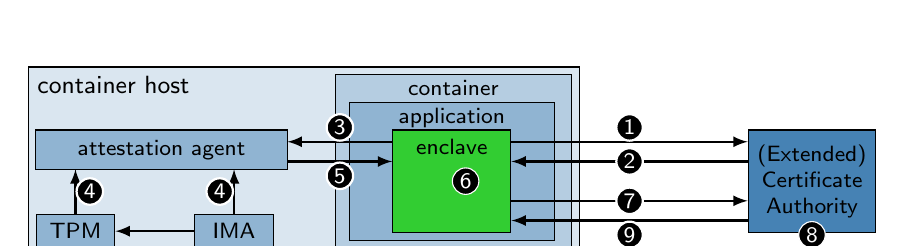
\begin{tikzpicture}[scale=1, every node/.style={scale=1}, node distance=2cm, font=\footnotesize\sffamily]
		\definecolor{bluebase}{RGB}{70,130,180}
		\colorlet{remotecolor}{bluebase!20}
		\colorlet{containercolor}{bluebase!40}
		\colorlet{vnfcolor}{bluebase!60}
		\colorlet{vmcolor}{bluebase!100}
		\colorlet{iascolor}{bluebase!80}
		\colorlet{enclavedcolor}{gray!80}
		\definecolor{enclavevcolor}{RGB}{50,205,50}
		\tikzset{cnc/.style={shape=circle,draw,inner sep=1pt, color=white,fill=black}}
		\tikzset{cn/.style={cnc,above}}
		\tikzset{cnr/.style={cn,right}}
		\tikzset{cnl/.style={cn,left}}
		\tikzset{cnb/.style={cn,below}}
		\tikzset{sa/.style={->,thick}}
		
		% Container host
		\node[minimum width=7cm,minimum height=2.4cm,fill=remotecolor,draw] (container host) at (0, 0) {};
		\node[below right] at (container host.north west) {\small container host};
		
		% Container
		\node[below left=0.1cm and 0.1cm,minimum width=3cm,minimum height=2.2cm,fill=containercolor,draw] (container) at (container host.north east) {};
		\node[below=-0.05cm] at (container.north) {\footnotesize container};

		% Application
		\node[above right=0.1cm and 0.18cm,minimum width=2.6cm,minimum height=1.75cm,fill=vnfcolor,draw] (vnf) at (container.south west) {};
		\node[below=-0.05cm] at (vnf.north) {\footnotesize application};
		
		% Enclave
		\node[above=0.1cm,minimum width=1.5cm,minimum height=1.3cm,fill=enclavevcolor,draw] (enclave) at (vnf.south) {};
		\node[below] at (enclave.north) {\footnotesize enclave};

		% Controller
		%\node[right=of container host,draw] (controller) {controller};
			
		% Verification Manager (Certificate Authority)
		\node[right=3cm of enclave,draw,align=center,fill=vmcolor,minimum height=1.3cm] (vm) {(Extended)\\ Certificate\\ Authority};
				
		% TPM
		\node[above right=0.1cm and 0.1cm,minimum width=1cm,minimum height=0.4cm,fill=vnfcolor,draw] (tpm) at (container host.south west) {TPM};
		
		% IMA
		\node[right=1cm of tpm,minimum width=1cm,minimum height=0.4cm,fill=vnfcolor,draw] (ima) {IMA};
		
		% Attestation agent
		\node[above right=-0.1cm and 0.1cm,minimum width=3.2cm,minimum height=0.5cm,fill=vnfcolor,draw,outer sep=0mm] (agent) at (container host.west) {attestation agent};
		\draw[->,thick] (ima.west) -- (tpm.east);

		% Numbered steps in attestation sequence.
		\coordinate (enclavesu) at ([yshift=5mm]enclave.west);
		\coordinate (enclavesd) at ([yshift=2.5mm]enclave.west);
		
		\draw[sa] ([yshift=5mm]enclave.east) -- node[cn] {1} ([yshift=5mm]vm.west);
		\draw[sa] ([yshift=2.5mm]vm.west) -- node[cnc] {2} ([yshift=2.5mm]enclave.east);
		\draw[sa] (enclavesu) -- node[cn] {3} (enclavesu -| agent.east);
		\draw[sa] (tpm.north) -- node[cnr] {4} (tpm.north |- agent.south);
		\draw[sa] (ima.north) -- node[cnl] {4} (ima.north |- agent.south);
		\draw[sa] (enclavesd -| agent.east) -- node[cnb] {5} (enclavesd);
		\node[cnr] at (enclave) {6};
		\draw[sa] ([yshift=-2.5mm]enclave.east) -- node[cnc] {7} ([yshift=-2.5mm]vm.west);
		\node[below=0.2cm of vm,cn] {8};
		\draw[sa] ([yshift=-5mm]vm.west) -- node[cnb] {9} ([yshift=-5mm]enclave.east);
	\end{tikzpicture}
	\caption{Enrollment steps in the application layer}
	\label{fig:apparchitecture}
\end{figure}

%============================================================================
\section{Implementation}
\label{sec:implem}
%============================================================================
To facilitate adoption and obtain reproducible results, we implemented the proposed solution using common open-source libraries and execution isolation features available on commodity platforms.
We used Open vSwitch (OvS), a popular software switch implementation and the Ryu and Floodlight SDN controllers, mainly due to their popularity and simple configuration.
In the remainder of this section, we first describe the implementation of TLSonSGX on the data plane.
Next, we describe the security mechanisms deployed on the application plane.

\subsection{TLSonSGX}
\label{subsec:tlsonsgx-impl}
The SGX programming model requires that applications deployed in SGX enclaves have an external component that can be called by other processes running on the operating system, and that in turn maps such calls to software in the enclave.
This external component is not part of the enclave and its integrity cannot be attested using the SGX integrity attestation mechanisms, thus is is considered \textit{untrusted};
in contrast, the code running in the enclave is considered \textit{trusted} once its integrity has been attested.
Following the SGX programming model, the untrusted code portion of the TLSonSGX library is a wrapper that maps OpenSSL external methods (used by Open vSwitch) internally into enclave calls (ECALLs).
The trusted portion of the code, contained within the SGX enclave, implements the ECALLs by utilizing the SGX trusted TLS library.
Support for TLS libraries in SGX varies and evolves continuously; 
we have chosen the mbed~TLS~\cite{mbedtls_sgx} library considering its sufficient support for SGX enclaves.

Considering that authentication keys and certificates are confined to the enclave, we modified OvS to use only a limited set of OpenSSL external methods that we subsequently implemented in TLSonSGX.
The OpenSSL library implements three data structures: \texttt{SSL\_METHOD}, \texttt{SSL\_CTX}, and \texttt{SSL}.

These data structures all contain crucial information for TLS connection security, therefore we create and confine them within the enclave.
The objects are passed by the OvS instance via an unmodified API using the external methods we implemented.
They are created, confined, and handled inside the enclave during the operation of the virtual switch, and hence discarded and not passed to ECALLs.
There is no one-to-one mapping in mbed~TLS for these three structures, hence we redefine these structures 
using mbed~TLS primitives (specifically the \texttt{mbedtls\_ssl\_config} and \texttt{mbedtls\_ssl\_context} data structures). 

The code in \texttt{stream-ssl.c} implements the interface between OvS and the OpenSSL library. 
We extended the OvS configuration script and \texttt{stream-ssl.c} with a new compilation flag, \texttt{SGX}.
If the \texttt{SGX} flag is set at compilation time, \texttt{stream-ssl.c} will use the TLSonSGX static library instead of the OpenSSL library.
Moreover, the sections of \texttt{stream-ssl.c} that load keys and certificates from the file system become redundant and are omitted.

\subsection{Application Plane}
\label{subsec:trustanchors:appplane}
On the application plane, the solution consists of three major components: the network application, the attestation agent, and the certificate authority.

The attestation agent is a service running on the container host, setup to listen to connections from containers running on the same host, as those are the only containers able to request a quote from this host.
The attestation agent can return both a copy of the measurement list, and a quote from the TPM.
The quotes are made over the appropriate PCR registers to capture the current configuration, together with a nonce to prevent replay attacks.
Interfacing with the TPM is implemented using the TrouSerS TSS library~\cite{trousers} on Linux.
Using an attestation agent reduced the code base of the containers, since they do not have to interface directly with a TPM or Linux IMA.

Next, the CA fulfills two goals.
First, it validates the integrity of the components by validating the quote, and compares the configuration and measurement list to known good values.
Second, if the two values match, the CA signs the applications CSR.
We implemented this using the OpenSSL C library to create the signature with a pre-configured root certificate.
This root certificate is distributed to the SDN controller, allowing it to validate the certificate chain.

The final component is the container application.
Using mbed~TLS~\cite{mbedtls_sgx}, we implemented an application that supports the attestation sequence described earlier, and communicates with both the attestation agent and the CA.
Once the attestation sequence is finished, the application can connect to an SDN controller using the credentials generated and confined within the enclave.

%============================================================================
\section{Evaluation}
\label{sec:eval}

\subsection{Testbed}
\label{subsec:testbed}
We evaluated the solution on the testbed described below (see Figure \ref{fig:testbed}).%comprising two VMs on a shared host platform , with the following specifications.
\paragraph{Hardware}
The host platform is a Lenovo Thinkpad T460s with a dual-core Intel Core\textsuperscript{TM} i7-6600U CPU clocked at 2.60GHz with SGX support.
VM\textsubscript{1} was created with 1 virtual CPU, and VM\textsubscript{2} with 2 virtual CPUs;
both VMs had 4 GB RAM, 30 GB of storage, and used virtio as vNIC.
We used Ubuntu 16.04.1 (with OvS and SGX drivers and SDKs) on both the host and VMs.
To enable the use of SGX within the VM environment, we created VM\textsubscript{2} using patched versions of QEMU and KVM provided by the SGX project\footnote{SGX Virtualization, \\\url{https://01.org/intel-software-guard-extensions/sgx-virtualization}} and Intel SGX SDK, v1.8. %\footnote{Released on March, 17th 2017}.

We enabled hyper-threading on the host platform, yielding 4 logical CPUs.
We pinned VM\textsubscript{1} to CPU 2 and VM\textsubscript{2} to CPUs 1 and 3 (same core).
In VM\textsubscript{2}, we pinned the virtual switch to CPU 1 and the traffic generator/sink and echo server to CPU 2, in order to reduce inter-core communication overhead~\cite{sekar:2012}. 
However, due to the limited number of cores on the host (2 cores) we were unable to implement strict CPU isolation by dedicating entire cores.
In~\S\ref{subsubsec:results_latency} we discuss the potential implications of this.

\paragraph{Software}
We used OvS release 2.6.0\footnote{Commit \texttt{4b27db644a8c8e8d2640f2913cbdfa7e4b78e788}}.
In VM\textsubscript{2}, we deployed OvS binaries compiled and linked with our TLSonSGX (as explained in~\S\ref{subsec:data-plane-trust}).
We created two network namespaces, each with a port connected to the OvS instance.

The CA uses OpenSSL 1.1.0d for TLS communication with OvS and to sign the OvS and the SDN controller certificates. 
We used OpenSSL, rather than TLSonSGX for the CA implementation for two reasons: 
(1) the CA implementation is trusted according to the threat model; 
and (2) to ensure interoperability between TLSonSGX (on the client side) and OpenSSL (on the server side).

We chose the Ryu SDN open-source controller as it supports TLS communication with OpenFlow switches\footnote{See Ryu 4.9 Documentation, \url{https://ryu.readthedocs.io/en/latest/tls.html}}.
It is written in Python and is widely used in research \cite{arbettu:2016} and in commercial products\footnote{See SmartSDN Controller, \url{https://osrg.github.io/ryu-book/}}.

\begin{figure}[t]
	\parbox{.5\linewidth}{
		\centering
		%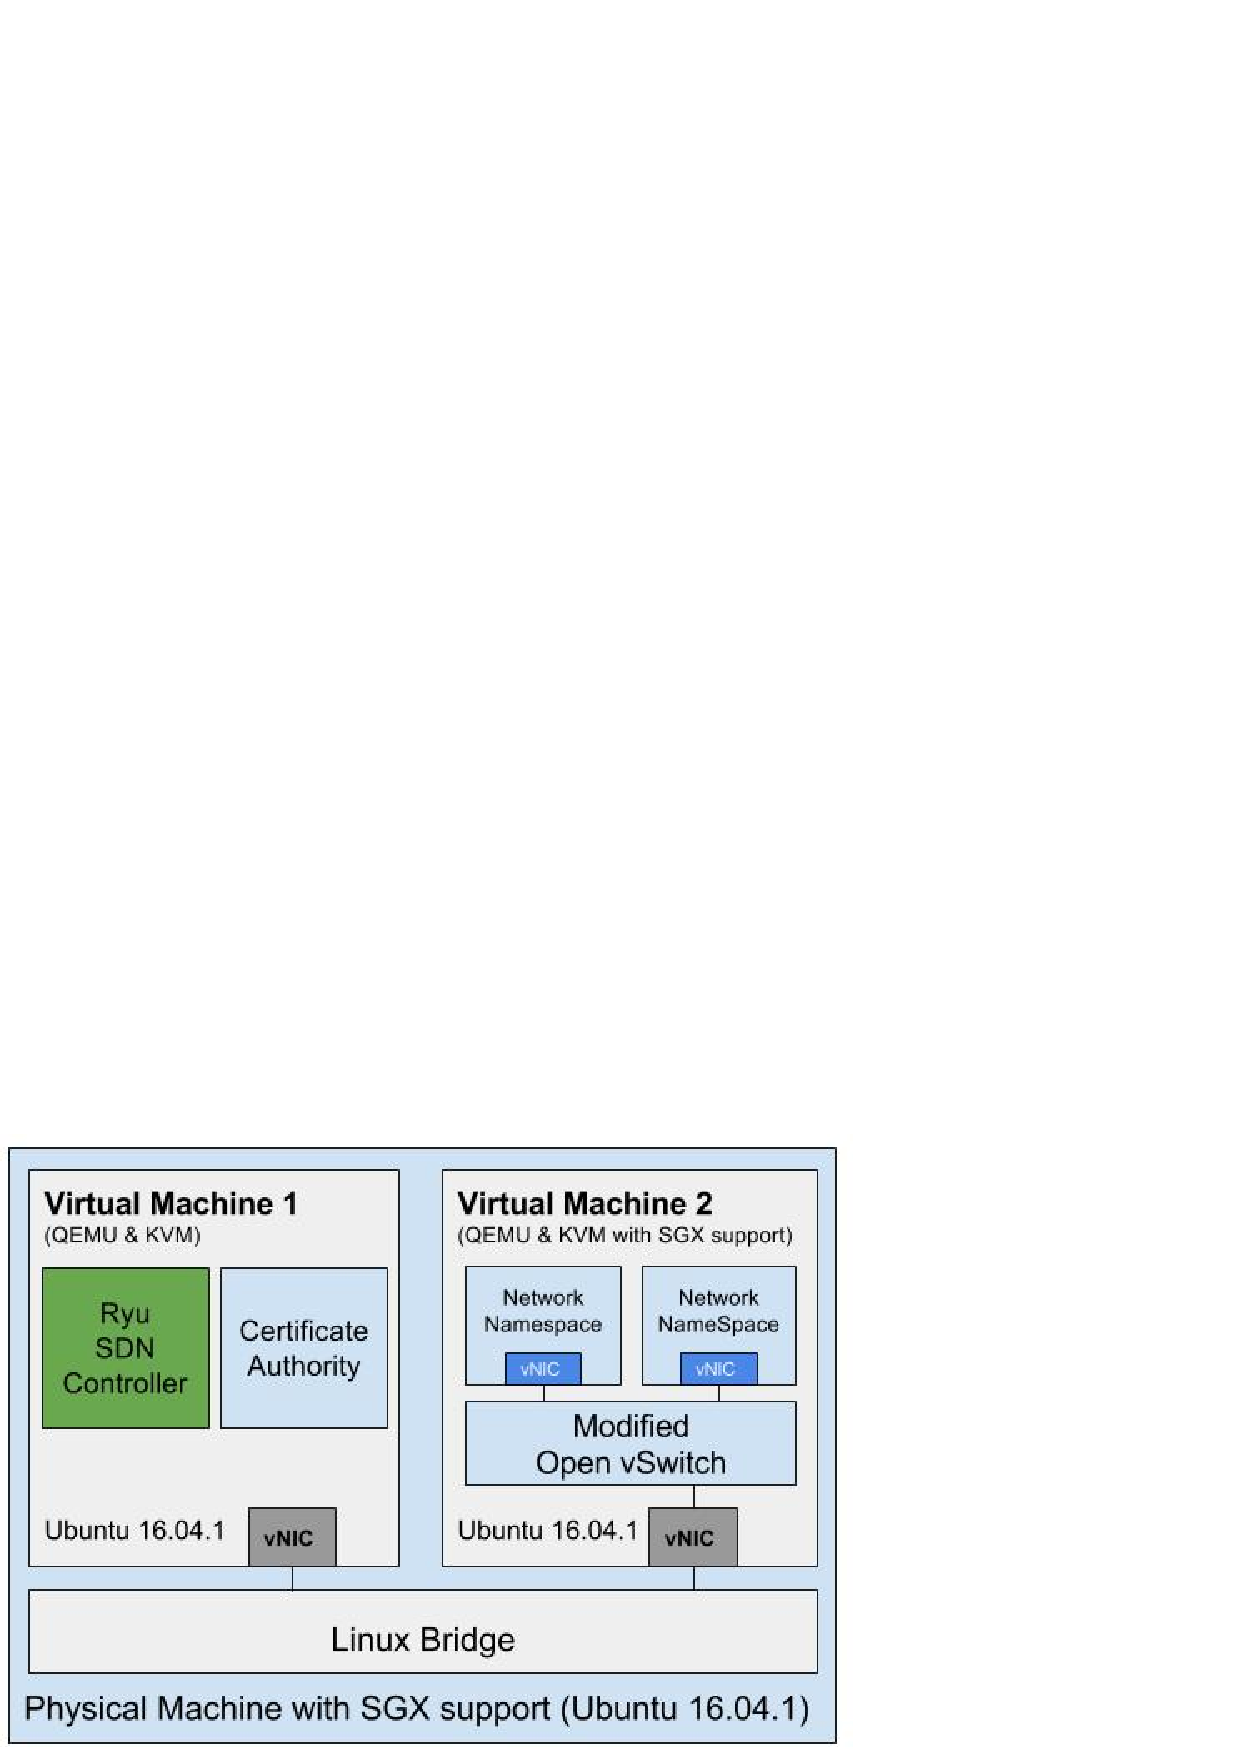
\includegraphics[width=1\linewidth]{testbed.jpeg}
		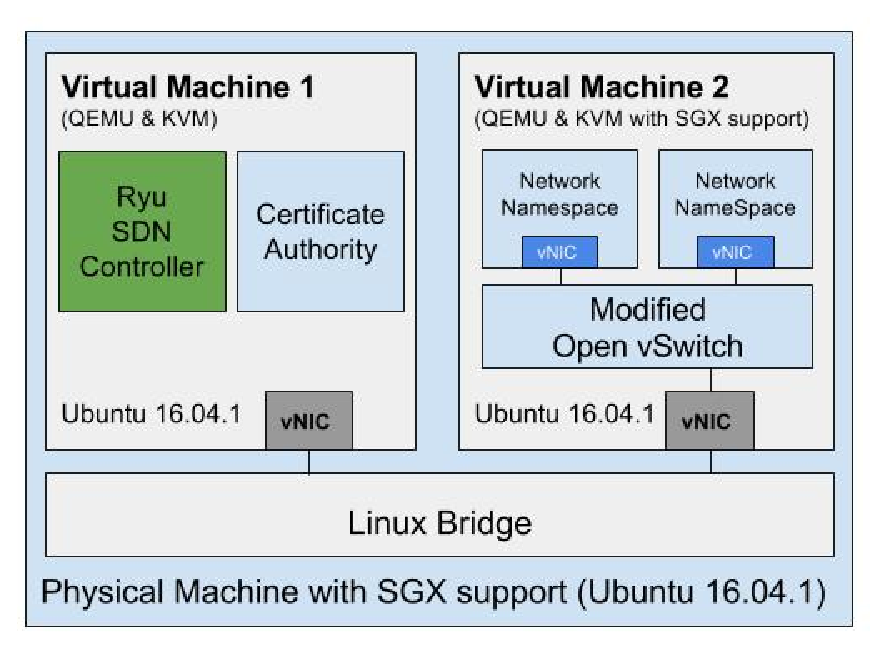
\includegraphics[width=1\linewidth]{testbed.eps}
		\caption{Testbed architecture}
		\label{fig:testbed}
	}%
	%\hfill
	\parbox{.5\linewidth}{
		\centering
		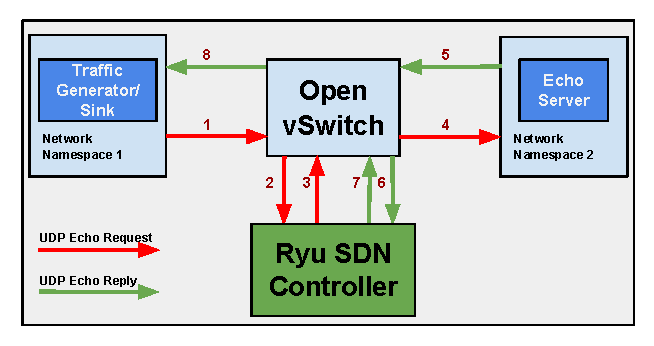
\includegraphics[width=1\linewidth]{Packet_Path.eps}
		\caption{UDP Packet Path}
		\label{fig:Packet_Path}
	}
\end{figure}

\subsection{Evaluation Targets}
\label{sec:planned_measurements}

\paragraph{SDN Controller Program}
In the SDN model, the virtual switch forwards the first packet in a new flow to the SDN controller.
The controller replies with a flow table update, the action to be executed by the switch to handle the packet, and the packet itself.
The virtual switch handles subsequent packets in the flow according to the newly installed rule in the flow table.

To exercise the communication between the SDN controller and the virtual switch and to capture latency measurements, we designed the SDN controller as a learning L2 switch, with a MAC address to port number mapping table.
To collect measurements of the controller-induced latency, the SDN controller sends no flow updates to the virtual switch (otherwise we would get one measurement per new destination).
As a result, the virtual switch sends all the packets in the flow to the SDN controller and the controller returns the packets to the virtual switch along with the action to send the packet through the corresponding port.

\paragraph{Performance Measurements}
\label{sec:performance_management}
We are primarily interested in the latency and the time required to generate key pairs and to obtain a signed certificate from the CA. 
When it comes to latency, the choice of traffic generators was limited to those that can provide latency measurements.
Moreover, such measurements require that clocks of both traffic source and sink are synchronized (or co-exist in the same host).
Having investigated several traffic generators (qperf~\footnote{See \texttt{qperf} man page}, pktgen~\cite{olsson:2005}, moongen~\cite{emmerich:2015}, and Click~\cite{morris:2000}), we chose Click due to its flexibility and versatility.

We implemented a traffic generator and sink using the Click Modular Router.
This allows us to measure round trip latency for UDP packets of varying sizes, at a rate of 500 Packets Per Second (pps) using the Click element \newline \texttt{StoreUDPTimeSeqRecord}.
Increasing the rate beyond that results in much higher latency variance (see \S\ref{subsubsec:results_latency}).

We deployed the traffic generator and sink in network namespace \textit{(i)} and a UDP echo server in network namespace \textit{(ii)}. 
The echo server echoes the received UDP packet back to the traffic generator and sink. 
The the two network namespaces communicate through Open vSwitch, as illustrated in Figure \ref{fig:Packet_Path}.
To benchmark the performance, we replicated the measurements in a clone of VM\textsubscript{2}, using a vanilla QEMU and 
KVM, with a default Open vSwitch implementation that uses OpenSSL.


\subsection{TLSonSGX Performance Evaluation}
\paragraph{Keys and Certificate Generation Time}
\label{section:keys_time}
This measurement concerns the time from \texttt{SSL\_library\_init} invocation in the Open vSwitch until the key pairs and signed certificate are loaded to the enclave's memory.
See measurement results in Table \ref{table:key_generation}.
There is no corresponding measurement in a vanilla Open vSwitch, since keys and certificates are handled manually~\cite{ovs_ssl}. 
However, as this operation is only executed once when \texttt{ovs-vswitchd} starts, the measurements show that there is little \textit{de facto} overhead introduced by the implementation. 

\begin{table}[tb]
	\parbox{.40\linewidth}{
		\centering
		\caption{Keys and certificate generation time. 1000 measurements.}
		\label{table:key_generation}
		\begin{tabular}{|l|l|}
			\hline
			\textbf{Mean}             &     0.344 seconds        \\ \hline
			\textbf{Variance}             &     0.0488        \\ \hline
			\textbf{1st Quartile} &     0.186 seconds       \\ \hline
			\textbf{Median}       &      0.276 seconds      \\ \hline
			\textbf{3rd Quartile}       &      0.434 seconds      \\ \hline
		\end{tabular}
	}
	\hfill
	\parbox{.55\linewidth}{
		\centering
		\caption{Packet rate vs. Average CPU utilization}
		\label{table:cpu_utilization}
		\renewcommand{\arraystretch}{}%{1.5		}
		\begin{tabular}{|c|c|c|}
			\hline
			\textbf{Packet Rate}  &  \textbf{ OpenSSL} & \textbf{TLSonSGX}      \\ \hline
			\ 500 pps &     25\% & 61\%        \\ \hline
			\ 1000 pps            &     40\% & 78\%        \\ \hline
			\ 2000 pps &     49\% & 96\%       \\ \hline
		\end{tabular}
	}
\end{table}

\subsubsection{Packet Round Trip Latency}
\label{subsubsec:results_latency}
In this section we discuss and analyze the packet round trip latency.
The measurements do not include the key generation time;
likewise, the time to establish a TLS session is not included, as it must already be established before packets can flow.
The TLS session remains active unless one of the two ends (Open vSwitch or SDN controller) terminates the session.

\paragraph{Packet Size}
\label{sec:packet_size}
The IP packet size received by the Open vSwitch from the traffic generator is bounded by the Maximum Transmission Unit (MTU) of the network namespace port connected to the Open vSwitch (1500 bytes in our tests).
Open vSwitch encapsulates the received packet 
in an OpenFlow \texttt{Packet In} message, adding an 18 bytes header \cite{openflowswitch}, that is in return encapsulated in a TLS record sent from the Open vSwitch to the SDN controller.
If the packet sent by the traffic generator is larger than the MTU, then it is fragmented and Open vSwitch handles it as two separate \texttt{Packet In} messages to the SDN controller. 

The TLS record adds a 5-byte header.
Depending on the cipher suite negotiated between the server and the client, a padding field (up to 15 bytes) is added, and the TLS record is appended with a Message Authentication Code (MAC) computed over the data.
In the handshake messages exchanged between Open vSwitch and the SDN controller in our tests, the negotiated cipher suite was \texttt{ECDHE-RSA-AES256-SHA}, which provides perfect forward secrecy through the use of an Elliptic Curve Diffie-Hellman key exchange \cite{rfc4492}, while the bulk encryption use 256-bit AES in CBC-mode with SHA-1 for MAC \cite{rfc3268}.

We measure the latency for increasing packet sizes ranging from 64 bytes up to 1408 bytes (in increments of 64 bytes), including the Ethernet and IP headers (minus the Cyclic Redundancy Check).
The upper limit is set to avoid subsequent fragmentation between the Open vSwitch and the SDN controller.

\paragraph{Packet Rate Selection and CPU Utilization}
We excluded outliers with a round trip latency over 2.5 milliseconds from the captured data: 5237 outliers when testing OpenSSL and 11622 outliers when testing TLSonSGX, out of 220000 samples for each implementation.
We investigated the CPU utilization to identify the cause of the outliers and the order-of-magnitude difference in the outlier numbers between the two implementations.
In both implementations, inside the VM, the first vCPU reaches 100\% utilization due to the Click packet generation process pinned to it, even at rates lower than 500 pps (i.e., 50, 100, 200 pps). 
However, the second vCPU, where \texttt{ovs-vswitchd} process is pinned, has a higher average CPU utilization when TLSonSGX is used compared to OpenSSL (see Table \ref{table:cpu_utilization}). 
Increasing the rate beyond 500 pps leads to increasing the second vCPU's utilization and average latency.
Thus, we chose 500 pps as a suitable and optimal maximum rate for further measurements and analysis.
Using SGX causes increased CPU utilization due to the overhead of transitioning to and from the memory enclave.

\paragraph{Latency and Packet Size}
The packet round trip latency measurements are plotted in a boxplot comparing TLSonSGX with the vanilla Open vSwitch with OpenSSL when forwarding UDP packets of a range of sizes (outliers were excluded, as stated above).
Figure \ref{fig:tcp_latency} shows a plot of latency versus packet size.

\begin{figure*}[t!]
\centering
\includegraphics[width=1.0\textwidth]{tlsonsgx_plot.eps}
\caption{UDP Packet Round Trip Latency vs. Packet Size}
\label{fig:tcp_latency}
\end{figure*}

Each box represents the data between first and third quartile, the thick line in the box represents the median.
The upper whisker is the minimum value between the data maximum and 3rd Quartile + 1.5*IQR, where IQR is the interquartile range.
The lower whisker is the maximum value between the data minimum and 1st Quartile - 1.5*IQR \cite{frigge:1989}.

A linear regression analysis of means shows that at zero byte TLSonSGX adds an overhead of 0.33 ms compared to OpenSSL.
In implementations the latency increases linearly with packet size;
we estimate this increase to 28 nanoseconds per byte for OpenSSL, and 182 nanoseconds per byte for TLSonSGX.
While the linear increase is consistent with our expectations (larger packets require more processing time),
the increase per byte is higher in TLSonSGX than in OpenSSL (154 nanoseconds per byte).
This, and the extra cost of 0.33 ms at zero byte are also expected due to the transition overhead to and from the memory enclave.
%Their numbers are as follows.

Once a packet is received at an Open vSwitch port from the network name space, \texttt{ovs-vswitchd} triggers \texttt{ecall\_ssl\_write} to encrypt and send the packet to the SDN controller,  while checking the SSL state (\texttt{ecall\_ssl\_get\_state}) before and after the write ECALL.
Since \texttt{ovs-vswitchd} uses non-blocking sockets, \texttt{ovs-vswitchd} keeps reading and returning from the socket (\texttt{ecall\_ssl\_read}), while comparing the SSL state before and after the read \newline (\texttt{ecall\_ssl\_get\_state}).
If a negative value is returned (WANT\_READ) from \texttt{ecall\_ssl\_read} then it triggers (\texttt{ecall\_ssl\_get\_error}) to retrieve the error code which indicates that the read call must be repeated and accordingly continue the loop.
If a positive value is returned, there is a response from the controller. 
The controller will respond with two packets: (1) the original packet itself; (2) the action needed by the switch to forward the packet to the second network name space.
The same flow will run during the return trip from the second network name space to the first one.


\begin{table}[t] % XXX: LNCS version
	\centering
	\small
	\caption{Analysis of packet latency (all measurements are in milliseconds**)}
	\label{table:analysis}
	\setlength{\tabcolsep}{2pt}
	\resizebox{\columnwidth}{!}{%
	\begin{tabular}{rcccccccc}
		\toprule
		& & & & \multicolumn{4}{c}{\texttt{ecall\_ssl\_}} & \multirow{2}{*}{\thead{Total \\enclave \\access}} \\
		\cmidrule{5-8}
		Size (B) & 
		\thead{TLSonSGX}  &
		OpenSSL & Diff & \texttt{read} & \texttt{write} & \texttt{get\_state}* & \texttt{get\_error}* & \\
		\midrule
		64 & 1.6500 & 1.2682 & 0.3817 & 0.0047 & 0.0646 & 0.0047 & 0.0043 & 0.2966 \\
		128 & 1.6667 & 1.2722 & 0.3944 & 0.0048 & 0.0676 & 0.0047 & 0.0043 & 0.3040 \\
		256  & 1.6820 & 1.2844 & 0.3976 & 0.0049 & 0.0725 & 0.0047 & 0.0043 & 0.3146 \\
		512  & 1.6852 & 1.2955 & 0.3897 & 0.0049 & 0.0828 & 0.0047 & 0.0043 & 0.3350 \\
		1024 & 1.6963 & 1.3145 & 0.3818 & 0.0049 & 0.1022 & 0.0047 & 0.0043 & 0.3740 \\
		\bottomrule
	\end{tabular}%
	}
	\raggedright {\textsf{\footnotesize* \texttt{ecall\_ssl\_get\_state} and \texttt{ecall\_ssl\_get\_error} are independent of packet size.}} \\
	\raggedright {\textsf{\footnotesize** Measurements captured in a different iteration than in Figure~\ref{fig:tcp_latency}.}}
\end{table}

To analyze and break down the time difference between OpenSSL and TLSonSGX, we traced the ECALLs indirectly called by \texttt{ovs-vswitchd} during the packet's round trip.
We measured the time consumed for each ECALL and repeated the measurement 10000 times per packet size.
Table \ref{table:analysis} lists the mean values for each of the four different ECALLs.
The last column in the table shows the sum of all ECALLs times per packet round trip. %, as explained above. 

We noticed that the duration of \texttt{ecall\_ssl\_write} is longer (and increases with packet size) than that of other ECALLs. 
This is because \texttt{ecall\_ssl\_write} is the only ECALL that writes from a buffer with a pointer outside the enclave (unprotected memory) to the enclave memory. 
All other ECALLs do the opposite. 
According to the manual, ECALLs that pass an external pointer into the enclave are slow, since a buffer is allocated inside the enclave memory\footnote{
Pointer Handling, {Intel {Software Guard Extensions SDK}}, \url{https://software.intel.com/en-us/node/708975}}. 
Before copying the contents of the external buffer into the enclave memory, the content and the size of the buffer referenced by the external pointer are verified for every call to prevent overwriting enclave code or data.

Recall from the system model (consistent with a typical SDN deployment) that only the first packet in the flow is sent to the SDN controller.
As a result, crafting a small enough first packet (64 bytes) allows to optimize the latency and reduce the time to add the flow rule in the Open vSwitch flow table.

\subsection{Application Plane Evaluation}
\label{subsec:application-evaluation}

In the application plane, we are mostly interested in performance measurement regarding the attestation time.
Every time a container is launched, both the container itself and the host it is running on must be attested.
In this section, we focus on measuring the attestation time for the proposed application plane design.
There are of course other relevant performance aspects, such as time required for the actual TLS connection to the controller, but we refer to previous work for such measurements \cite{girtler:2017}.

\begin{table}[h] % XXX: LNCS version
	\centering
	\caption{Attestation Time in Application Plane for various stages of the attestation sequence. Stages with execution time $< 0.010 \text{ s}$ removed.}
	\label{tbl:apptotalatttime}
	%\renewcommand{\arraystretch}{}%{1.5}
	\setlength{\tabcolsep}{3pt}
	\begin{tabular}{lrrr}
		\toprule
		Stage & Mean & Variance & Median \\
		\midrule
		TPM quote              & 0.332 s & 0.000159 & 0.335 s \\
		Key generation         & 0.326 s & 0.050746 & 0.266 s \\
		CSR signing            & 0.011 s & 0.000002 & 0.010 s \\
		\midrule
		Total attestation time & 0.686 s & 0.050849 & 0.622 s \\
		\bottomrule
	\end{tabular}
\end{table}

The benchmarks were made by repeatedly launching the application which triggers the attestation. 
We ran 1000 tests, and calculated the mean and median values of the total attestation time (see results in Table~\ref{tbl:apptotalatttime}).
As seen from the table, the attestation time is well below one second in the average case.
Breaking down the execution time to various stages of the attestation, and presenting those with an execution time of $\ge 0.010 \text{ s}$, we see that the majority of the attestation time is spent in two different stages: (1) waiting for the TPM chip to generate the quote, and (2) generating the private key within the enclave. 
Stage (1) is implemented in the TPM chip itself, while stage (2) depends on the size and type of key generated. A 2048-bit RSA key was used for the measurements presented above.
We also note that our current implementation is not optimized, and it may be possible to reduce the execution time even further.
%One fairly straightforward optimization for future work could be to generate the private key and waiting for the TPM quote in parallel.

%============================================================================

\section{Related Work}
\label{sec:related-work}
%============================================================================

\subsection{Isolating Network Elements}
\label{subsec:effective-network-element-isolation}
Protecting the sensitive code and data of network elements is a topic of active on-going research.
Jacquin proposed an architecture that used a hardware root of trust to remotely attest the integrity of virtualization hosts in SDN infrastructure~\cite{jacquin:2015}.
Furthermore, commodity TEEs were used in case studies on securing network applications~\cite{kim:2015,shih:2016}, implemented using OpenSGX, an emulator of SGX~\cite{jain:2016}.
TruSDN is a framework for bootstrapping trust in an SDN infrastructure implemented using OpenSGX~\cite{paladi:2016b}.
It supports secure provisioning of switches in SGX enclaves, a secure communication channel between switches and SDN controller, and secure communication between endpoints in the network using session keys that are generated per flow and used only during the lifetime of the flow.
Similarly, \textit{Trusted Click}~\cite{coughlin:2017} explores the feasibility of performing network processing in SGX enclaves.

\textit{SCONE} enables operators to protect confidentiality and integrity of computation in application containers against an adversary with root access to the container host~\cite{arnautov:2016}.
SCONE achieves this by deploying containers within SGX enclaves and relies on a \texttt{libc} library ported to the SGX environment to reduce performance impact of context switches between SGX enclaves and the underlying OS, at the cost of expanding the TCB.

Our solution addresses both confidentiality of long-term credentials and session keys, as well as integrity of the network element platform. %host where the network elements execute.
In particular, we enable network elements on remotely attested hosts to protect their communication with the network controller using a TLS library and credentials in a local SGX enclave.
This allows us to protect core assets with insignificant performance overhead and minimal changes to network element implementations.
Porting entire applications into SGX enclaves - as proposed in the related work above - expands the attack surface to both software vulnerabilities and side-channel attacks.
We avoid this by only porting to the enclaves a minimal TCB of the network elements.
We reduce the TCB by only confining the TLSonSGX library, credentials, and TLS session information to the enclave.


\subsection{Enrolling Network Elements}
\label{subsec:enrollment-and-key}
According to \cite{paladi:2015b}, incomplete or incorrect network views are an attack vector in SDN deployments.
The Secure Network Bootstrapping Infrastructure (SNBI) protocol~\cite{snbi} bootstraps secure communication channels of network elements and controllers and provisions the keys required for secure communication.
To enable connectivity to the network devices, SNBI assigns unique IPv6 addresses (based on the unique device identifier) or and bootstraps devices with the required keys.
However, the SNBI protocol is not resistant against impersonation attacks on network elements and fails to specify a protocol for software network elements with similar security features.
We address the shortcomings of SNBI by attesting the integrity of the trusted computing base of the platforms hosting network elements prior to provisioning authentication credentials;
the credentials are stored in a secure enclave and as described in~\ref{subsec:tlsonsgx-impl}, never leave the enclave.


\subsection{TLS Implementations for SGX}
\label{subsec:tls-for-sgx}
There are several known TLS libraries ported to SGX enclaves.
TaLoS~\cite{aublin:2017} terminates TLS communication inside the container enclave by providing a port of LibreSSL library into SGX and thus maintaining OpenSSL API, including APIs to set private keys and certificates from outside the enclave. 
In this paper, keys and certificates are maintained inside the enclave and no APIs are exposed to manipulate them.
Furthermore, TaLoS %was released in March 2017 and thus it 
was not available at the time of writing.

Initially, mbed TLS was the only available port of a TLS library into SGX in Linux \cite{mbedtls_sgx}. % \footnote{TLS for SGX: a port of mbedtls, \url{https://github.com/bl4ck5un/mbedtls-SGX}}. 
Intel \cite{sgxssl} and wolfSSL \cite{wolfSSL} provided a port to Linux in May 2017 and June 2017 respectively. 
However, none of these three provided an unmodified OpenSSL API that is exposed outside the enclave.
%Moreover, Intel\textsuperscript{\textregistered} SGX SSL library supports only a subset of OpenSSL APIs available only within the enclave and not exposed outside the enclave.
Thus, none of the TLS libraries for SGX enclaves expose the required functionality.
We implemented TLSonSGX to address the lack of usable implementations. 
TLSonSGX implements a wrapper around mbed TLS Trusted SGX library that exposes the OpenSSL APIs (that are needed for Open vSwitch TLS operations) outside the enclave.

\label{subsec:attacks-on-tls-sgx}
Popular TLS libraries with support for execution in SGX enclaves (OpenSSL, GnuTLS, mbed TLS, WolfSSL, LibreSSL) are vulnerable to Bleichenbacher attacks~\cite{bleichenbacher:1998} and a modified version padding oracle attacks~\cite{vaudenay:2002} on branch level, cache line level and page level~\cite{xiao:2017}.
Such attacks can be mitigated by using the Diffie-Hellman (DH) key exchange instead of RSA-based key exchanges and \textit{Authenticated Encryption with Associated Data} (AEAD) mode for encryption~\cite{xiao:2017}.
TLSonSGX is compatible with the mitigation suggested in \cite{xiao:2017} and can be configured to enforce DH key exchanges and AEAD encryption mode.


%============================================================================
\section{Limitations and Future Work}
\label{sec:future_work}

We implemented a prototype and tested it using one dual-core laptop and used VMs with SGX support to host the virtual switches, the SDN controller, and network namespaces (See in~\S\ref{subsec:testbed}). 
While this sufficient to demonstrate the feasiblity of TLSonSGX and compare it to OpenSSL, the platform choice 
limited possible performance measurements.
Dedicated multi-core platforms, or cloud resources, with SGX support could be used to refine the performance measurements.

The current implementation supports only one virtual switch connecting multiple VMs per physical host, as only one SSL context is created and kept inside the enclave. 
This can be improved by introducing support for multiple switches per host by extending the library to support multiple SSL contexts. 
TLSonSGX could also be extended to protect the flow table %(stored in unprotected memory)
or OVS database content %(stored as a file in the disk)
from tampering by storing them in the enclave. 

For keys and certificates to survive host reboots, the enclave could deploy sealing mechanisms to seal the enclave, i.e. encrypt it, export it from the enclave, and store it on the local hard disk. 
We did not prioritize this, as generating new keys and obtaining a new certificate takes approximately 0.3 seconds (See~\S\ref{section:keys_time}).

%============================================================================


%============================================================================
\section{Conclusion}
\label{sec:trustanchors:conclusion}
Protecting network elements on the data and application planes is essential for the security of SDN deployments and the network isolation between tenants.
However, both state of art network elements and the underlying platforms are vulnerable to software attacks, potentially exposing authentication credentials stored in plaintext.
To address this, we implement the TLSonSGX library that provides a secure and scalable mechanism for network elements to generate keys and obtain signed certificates, while keeping them secure within a memory enclave.
TLSonSGX confines all the TLS connections to the SDN controller within the enclave to ensure that keys, certificates, and session data remain inaccessible outside the enclave.
We complement TLSonSGX with additional mechanisms to asses the network element trustworthyness and apply the approach on both data- and application planes.

Our evaluation results show that TLSonSGX does not significantly impact the time to generate credentials and only adds an insignificant overhead when processing the first packet in each flow.
TLSonSGX reduces the TLS configuration overhead and improves the security of SDN deployments.

%============================================================================



%=======================WE WILL ADD ACKNOWLEDGEMENTS IN THE CAMERA READY VERSION=====================================================
%============================================================================
\subsubsection*{Acknowledgements.}
\label{sec:acknowledgements}
%============================================================================

This research was conducted within the 5G-ENSURE and COLA projects and received  funding  from  the European Union's Horizon 2020 research and innovation programme, under grant agreements No 671562 and 731574.
%=======================WE WILL ADD ACKNOWLEDGEMENTS IN THE CAMERA READY VERSION=====================================================

%\bibliographystyle{splncs04}
%\bibliography{bt-bibliography}

%\end{document}

{\raggedright
	\printbibliography[segment=\therefsegment,heading=subbibliography]
}

}


\fi

\ifpaperIV
\newrefsegment
\addtolength{\apa}{2cm}
\fancyhead[RE]{\paperref{ch:recsys}: \paperIVtitle}
\chapter[\paperIVtitle]{\texorpdfstring{%
		\paperIVtitle}{%
		\paperIVtitle}}

\label{ch:recsys}
\paperRemark{This is the full version of the paper below.
	This version contains an extended background description, and a more detailed motivation behind choices in the implementation as well as evaluation.

	\paperIVref}

{

%\documentclass{llncs}
%\usepackage{amsmath}
%\usepackage{amssymb}
%\usepackage{bm}
%\usepackage{booktabs}
%\usepackage{enumitem}
%\usepackage{tikz}
%\usetikzlibrary{shapes,arrows,calc,positioning,shapes.geometric}
%\usepackage{url}
%\usepackage{xcolor}
%\usepackage{cite}
%\usepackage{multirow}
%\usepackage{makecell}
%\usepackage{tabularx}
%\usepackage{multicol}
%\usetikzlibrary{arrows,backgrounds,calc,positioning}

%\title{A Recommender System for User-Specific Vulnerability Scoring}
%\author{Linus Karlsson, Pegah Nikbakht Bideh, Martin Hell}
%\institute{Lund University, Department of Electrical and Information Technology, Sweden 
%	\email{\{linus.karlsson, pegah.nikbakht\_bideh, martin.hell\}@eit.lth.se }
%}

% some nice shortcuts to reduce typing.
\newcommand{\simsf}{\mathsf{sim}}
\newcommand{\updatesf}{\mathsf{update}}
\newcommand{\mersf}{\mathsf{mer}}

\newcommand{\bmv}{\bm{v}}
\newcommand{\bmw}{\bm{w}}
\newcommand{\bmu}{\bm{u}}
\newcommand{\bmuhat}{\bm{\hat{u}}}

% Counter for the nice circled thingies.
\newcounter{blockcntno}
\renewcommand{\theblockcntno}{\alph{blockcntno}}
\newcommand{\blockcnt}[1]{\refstepcounter{blockcntno}\label{#1}}

% For the nice circled thingies with black background.
%\newcommand*\circled[1]{\tikz[baseline=(char.base)]{
%            \node[shape=circle,draw,inner sep=1pt,color=white,fill=black,minimum size=0.4cm] (char) {\ref{#1}};}}

% The same with white background.
%\newcommand*\circled[1]{\tikz[baseline=(char.base)]{
%            \node[shape=circle,draw,inner sep=1pt,color=black,fill=white,minimum size=0.4cm] (char) {\ref{#1}};}}
% Third option which just replaces it with (a) (b) parentheses if we want to be really boring and non-creative ;)
\newcommand*\circled[1]{(\ref{#1})}

%\begin{document}
	
%\maketitle

\section*{Abstract}
With the inclusion of external software components in their software, vendors also need to identify and evaluate vulnerabilities in the components they use.
A growing number of external components makes this process more time-consuming, as vendors need to evaluate the severity and applicability of published vulnerabilities.
The CVSS score is used to rank the severity of a vulnerability, but in its simplest form, it fails to take user properties into account.
The CVSS also defines an environmental metric, allowing organizations to manually define individual impact requirements.
However, it is limited to explicitly defined user information and only a subset of vulnerability properties are used in the metric.
In this paper we address these shortcomings by presenting a recommender system specifically targeting software vulnerabilities.
The recommender considers both user history, explicit user properties, and domain based knowledge.
It provides a utility metric for each vulnerability, targeting the specific organization's requirements and needs.
An initial evaluation with industry participants shows that the recommender can generate a metric closer to the users' reference rankings, based on predictive and rank accuracy metrics, compared to using CVSS environmental score.


%%%%%%%%%%%%%%%%%%%%%%%%%%%%%%%%%%%%%%%%%%%%%%%%%%%%%%%%%%%%%%%%%%%%%%%%%%%%%%%%%%%%%%%%%%%%%%%%%%%%%%%%%%%%%%%%%%%%%%%

\section{Introduction}
The current software development landscape shows a trend towards increasing reuse of existing code.
Products are constructed by using already existing libraries and software, such as OpenSSL, libxml, and many others.
A report \cite{synopsis:2018}, found that in the scanned applications, on average 57\% of the code base was open source.
However, as a maintainer of products, vendors need to identify vulnerabilities in the components they use.
As the number of external components increases, the workload on developers to identify vulnerabilities and update these components grows.
At the same time, many vendors already have a hard time to identify and evaluate vulnerabilities, for example in IoT companies
\cite{host:2018}. % TODO: add more details, find other research that supports us? look eg in hösts paper.

Updating a component introduces a cost, since it requires a new release cycle to be completed.
This includes building, quality assurance, and the distribution of the new release to the end-users' devices.
Therefore, vendors would like to patch only vulnerabilities which are relevant to the product.

The Common Vulnerability Scoring System (CVSS)~\cite{cvss2spec,cvss3spec} defines a severity ranking for vulnerabilities.
The base score does not take into account individual preferences of users. Instead, CVSS has an environmental metric which can be used to modify the base score such that it represents user dependent properties of vulnerabilities. It will rewrite the confidentiality, integrity, and availability metrics both to adjust them according to measures already taken by the organization, but also to capture the actual impact such loss would have on the organization. As this will differ between organizations, such a modified metric will better reflect the actual severity of a vulnerability to that organization. 

The environmental metrics must be evaluated on a per vulnerability basis and are handled manually. This is both time consuming, error prone, and can lead to inconsistencies in case there are several vulnerabilities and they are handled by different analysts. Moreover, the environmental metric, though unique for the organization, only constitutes the sub-metrics available in the base score. Additional information that might affect the organization is not covered.

Recommender systems work by analyzing information about user preferences, and combine this with information about items, or with the history of other users.
Their goal is to output recommendations targeting the specific user.

%In this paper, we focus on the prioritization problem by designing a recommender system for vulnerabilities.
In this paper, we explore ways to improve measuring how a vulnerability affects an organization. Using machine learning techniques applied to recommender systems, we combine different properties and metrics in order to capture vulnerability data and map it to requirements of the specific organization. Compared to CVSS environmental metrics, our method provides several advantages.

First, the requirements for the organization is derived by combining explicit requirements with requirements learned from previous analysis of vulnerabilities. This data driven approach will not only use personal preferences, but also take into account how real vulnerabilities have been evaluated previously. Such learned data is able to capture information that might be overseen by analysts, or that are difficult to express. Second, our approach is general and is not restricted to a certain group of properties. It can be amended with new metrics if needed, focusing on metrics relevant for the given organization or device. 

Our goal is to design a recommender that provides a personalized severity assessment based on a user profile.
The profile is both explicit, based on the users' own choices, and implicit as the recommender learns from the users' previous actions.
We also support inclusion of domain knowledge into the system and discuss how the different parts can be weighted, following a heuristic approach. Suitable similarity functions are used to form a utility function that outputs the personalized severity assessment. The recommender is also evaluated using participants from the industry. Though the evaluation is small scale, the results indicate that our recommender system is able to provide severity information that is closer to the users' actual preferences than the CVSS environmental score.

The remainder of this paper is structured as follows: in Section~\ref{sec:recsys:background} we describe the necessary background of recommender systems and vulnerabilities.
In Section~\ref{sec:model} the proposed model is described, which is followed by the implementation of the model in Section~\ref{sec:implementation}.
The recommender is evaluated in Section~\ref{sec:recsys:evaluation}.
Related work is discussed in Section~\ref{sec:relatedwork}.
Finally, the paper is concluded in Section~\ref{sec:recsys:conclusions}.

%%%%%%%%%%%%%%%%%%%%%%%%%%%%%%%%%%%%%%%%%%%%%%%%%%%%%%%%%%%%%%%%%%%%%%%%%%%%%%%%%%%%%%%%%%%%%%%%%%%%%%%%%%%%%%%%%%%%%%%

\section{Recommenders and Vulnerability Severity Ratings} \label{sec:recsys:background}

Generally, the goal of a recommender is to present recommendations of \emph{items} to a set of \emph{users}. An item can be for example a movie, a song, or a website. 
The idea is that the recommender should present a subset of items to the user, such that the user finds this subset relevant. The subset is found by matching user preferences or activity  using a learnt profile and sometimes other similar users' activity. In a shopping scenario, the added value for the user also leads to higher sales.
%Some recommenders can increase sale while others can add value to the user.
%For e-commerce sites, this can increase the sales by presenting items the customer is likely to buy.
%In other cases, such as movie or music recommendations on streaming services, the recommender is instead something that adds value to the users.
%It helps users to more easily navigate the large collection of media available.
In this paper, the goal of the recommender is to add value to an end-user by tailoring the severity score for vulnerabilities.

Recommender systems can be divided into three major categories \cite{aggarwal:2016}: knowledge-based systems, content-based systems, and collaborative filtering.
%Each type has different properties and different advantages and drawbacks.

A knowledge-based recommender system
can be used in cases where ratings of items are not available, e.g., rarely used or bought items.
%This includes items which are bought rarely, such as luxury goods.
It finds similarities between user requirements and item descriptions.
In other words, a knowledge-based recommender allow users to specify desired domain-specific properties of items, and the recommender tries to find suitable items.

In content-based systems,
item descriptions are used for recommendations and user ratings are combined with item information.
One advantage of content-based systems is that when a rating is not available for an item, items with similar attributes that have been rated by the user can be used to make recommendations.
On the other hand, because the lacking history of ratings for new users, they are not effective at providing recommendations for new users. 

Collaborative filtering systems
use collaborative ratings provided by multiple users to make recommendations. %Rating metrics in collaborative filtering are sparse. This means that in large set of items, if only a small fraction of them have ratings, unspecified or unobserved ratings can be imputed by observed ratings. For example, 
If two users have similar taste of ratings for many items, this similarity is identified. When only one of them has specified a rating, the other user can receive a similar rating. 

Other than the types above,
recommendations can be generated from domain-specific knowledge.
This generates recommendations for a specific field of knowledge,
and is designed specifically to handle data for that domain.
%In addition to the recommender systems above, there is another type of recommender system called domain-specific knowledge system. This type of recommender does not generate user based recommendations, in fact it generates recommendations based on a specific field of knowledge which can be applied to all users.  

The above recommenders works well in defined scenarios. Knowledge-based systems are efficient in cold-start settings, while collaborative methods works well when a lot of ratings are available. Various features of different recommenders can be combined in hybrid systems for better performance. 

Many vulnerabilities are reported and given a CVE identifier. The CVE system thus provides a centralized repository for vulnerabilities. As an example, in 2018, more than 16,500 vulnerabilities were added to the National Vulnerability Database (NVD). For each vulnerability, NVD also provides a severity score. This score, denoted the base score, uses exploitability and impact submetrics in order to define a severity score between 0--10. This score is made to be reproducible and organization independent. Instead, the environmental score can be used to adapt the base score to an organization's requirements and needs. In this paper, a recommender system has been applied to CVEs, and the performance is compared to the environmental metric.    
%%%%%%%%%%%%%%%%%%%%%%%%%%%%%%%%%%%%%%%%%%%%%%%%%%%%%%%%%%%%%%%%%%%%%%%%%%%%%%%%%%%%%%%%%%%%%%%%%%%%%%%%%%%%%%%%%%%%%%%

\section{System Model} \label{sec:model}

During the design of a recommender system for vulnerabilities, several requirements should be fulfilled. The following requirements have been identified: 1) The recommender should give reasonable recommendations for new users of the system, and thus avoid the cold-start problem of recommender systems. 2) It should allow the user to select certain preferences that the system will honor. 3) It should expose a meaningful subset of user preferences to the user. 4) It should learn from user actions, so that future recommendations are as relevant as possible to the user. To avoid privacy concerns, only the user's own actions are considered. Thus, methods based on collaborative filtering will not be considered in this paper.

% \begin{enumerate}
% 	\item The recommender should give reasonable recommendations for new users of the system, and thus avoid the cold-start problem of recommender systems.
% 	\item The recommender should allow the user to select certain preferences that the system will honor.
%     \item The recommender should expose a meaningful subset of user preferences to the user.
% 	\item The recommender should learn from user actions, so that future recommendations are as relevant as possible to the user. To avoid privacy concerns, only the user's own actions are considered.
% \end{enumerate}

We first note that no single class of recommender system can fulfill all requirements.
Instead, we propose a hybrid recommender based on three parts.
The first is a \emph{domain-based} subsystem which provides domain-specific knowledge unique to a recommender for vulnerabilities. The second part is a \emph{knowledge-based} subsystem which allows the user to select certain user preferences that they are interested in. Lastly, the third part is a \emph{content-based} subsystem which learns from the user's previous actions to provide more meaningful recommendations for each user. %Methods based on collaborative filtering will not be considered further in this paper due to potential privacy issues. 
%when recommendations are based on other users' actions.

\tikzstyle{block} = [rectangle, draw, fill=blue!20, text width=6em, text centered, rounded corners, minimum height=4em]
\tikzstyle{line} = [draw, -latex']
\tikzstyle{cloud} = [draw, ellipse,fill=red!20, node distance=3cm, minimum height=2em]
\tikzstyle{rec} = [rectangle, draw, fill=yellow!50, text width=5em, text centered, minimum height=4em]

\begin{figure}[btp]
	\centering
	\begin{tikzpicture}[scale=0.9, every node/.style={scale=0.9}, node distance = 2cm, auto, font=\small\sffamily,
	database/.style={
		cylinder,
		cylinder uses custom fill,
		cylinder body fill=yellow!50,
		cylinder end fill=yellow!50,
		shape border rotate=90,
		aspect=0.25,
		draw
	},
	% black circle.
	%cnc/.style={shape=circle,draw,inner sep=1pt,color=white,fill=black,minimum size=0.4cm}]
	% white circle
	cnc/.style={shape=circle,draw,inner sep=1pt,color=black,fill=white,minimum size=0.4cm}]
	% Place nodes
	\node [block] (init) {User requests recommendations for a set $c$ of vulnerabilities};
	%\node [cnc] {b} at (0,0);
	\node[cnc] at (init.north west) {\blockcnt{blk:ureq}\ref{blk:ureq}};
	
	\node [block, below of=init, node distance=2.5cm] (dmknowledge) {Domain knowledge $\bm{w}$};
	\node[cnc] at (dmknowledge.north west) {\blockcnt{blk:dmknowledge}\ref{blk:dmknowledge}};
	%\node [rec, above left of =dmknowledge, node distance=3.5cm] (domain) {Domain knowledge};
	\node [block, right of=dmknowledge, node distance=2.8cm] (coeff) {Subsystem weights $\bm{\alpha}, \bm{\beta}, \bm{\gamma}$};
	\node[cnc] at (coeff.north west) {\blockcnt{blk:coeff}\ref{blk:coeff}};
	\node [block, right of=coeff, node distance=2.8cm] (profile) {Fetch user profile $\bmu$, $\bmuhat$};
	\node[cnc] at (profile.north west) {\blockcnt{blk:profile}\ref{blk:profile}};
	\node [block, right of=profile, node distance=2.8cm] (feature) {Fetch feature data for each CVE};
	\node[cnc] at (feature.north west) {\blockcnt{blk:feature}\ref{blk:feature}};
	\node [database, above=1cm of feature] (db) {Vulnerability db};
	\node [block, below of=dmknowledge, node distance=2cm] (combine) {Calculate utility $U$ for each CVE in $c$};
	\node[cnc] at (combine.north west) {\blockcnt{blk:combine}\ref{blk:combine}};
	%\node [block, below of=combine, node distance=2cm] (stop) {Rank value per CVE};
	\node [database, above=1.8cm of profile] (pdb) {User profile db};
	% Draw edges
	\path [line] (init) -- (dmknowledge);
	\path [line] (dmknowledge) -- (combine);
	%\path [line] (combine) -- (stop);
	%\path [line] (combine.south) -- node {ranking} ++(0,-0.5cm);
	\path [line] (init) -- (coeff);
	\path [line] (init) edge[bend left=30] node[below] {} (profile);
	\path [line] (init) edge[bend left=25] node[below] {$c$} (feature);
	\path [line] (coeff) -- (combine);
	\path [line] (profile) edge[bend left=10] (combine);
	\path [line] (feature) edge[bend left=15] (combine);
	
	\path [line,dashed] (pdb) -- (profile);
	\path [line,dashed] (db) -- (feature);
	
	%\path [line,dashed] (domain) edge[bend right=20] (dmknowledge);
	\end{tikzpicture}
	\caption{Flow chart of recommendation generation}
	\label{fig:userreqrec}
\end{figure}

\subsection{Overall Recommender System Design}
An overview of the recommendation generation process can be seen in Fig.~\ref{fig:userreqrec}.
When a user requests recommendations for a set $c$ of vulnerabilities, the feature data, domain-specific knowledge, user profiles, and weights are fetched from their respective storage.
Each of these parts will be described in details in the following sections.
These pieces will then be combined in the actual recommender, which then outputs recommendations in the range $[0,1]$.
Such a value is generated for each vulnerability in the set $c$ of user requested vulnerabilities.
A higher value means that a vulnerability is more relevant to the user.

Our hybrid recommender system learns user preferences based on the user's interaction with vulnerabilities.
An overview of the rating procedure is shown in Fig.~\ref{fig:userraterec}.
First, the user rates a vulnerability based on their own preferences.
While such a rating can be of any form, this paper only considers positive feedback.
Next, the current user profile is updated with the new information, so that a new user profile estimated called $\bmuhat$ is stored in the user profile database.
The profile update procedure will be explained in Section~\ref{sec:userprofileupdate}. 

\begin{figure}[tb]
	\centering
	\begin{tikzpicture}[scale=0.9, every node/.style={scale=0.9}, node distance = 2cm, auto, font=\small\sffamily,
	database/.style={
		cylinder,
		cylinder uses custom fill,
		cylinder body fill=yellow!50,
		cylinder end fill=yellow!50,
		shape border rotate=90,
		aspect=0.25,
		draw
	}]
	% Place nodes
	\node [block] (init) {User marks vulnerability as interesting};
	
	\coordinate[right=2cm of init] (rinit);
	%\node [cloud, above=0.1cm of rinit] (u) {$u$};
	%\node [cloud, below=0.1cm of rinit] (v) {$v$};
	
	%\node [block, below of=init, node distance=2.5cm] (historian) {Store raw user interaction in historian};
	%\node [database, right of =historian, node distance=5cm] (db) {Historian};
	\node [block, below of=init, node distance=2cm] (update) {Update user profile};
	\node [rec, right of =update, node distance=4cm] (profile) {Profile updater};
	\node [database, right of =profile, node distance=4cm] (userdb) {User profile db};
	
	% Draw edges
	%\path [line] (init) -- (historian);
	%\path [line] (historian) -- (update);
	\path [line] (init) -- (update);
	
	%\path [line,dashed] (u) -- (init.east |- u);
	%\path [line,dashed] (v) -- (init.east |- v);
	
	%\path [line,dashed] (historian) -- node {$u, v, \text{datetime}$} (db);
	
	%\path [line,dashed] (update) edge[bend left=40]  node {} (profile);
	\path [line,dashed] (update) edge node {} (profile);
	\path [line,dashed] (profile) edge[bend right=40] node[below] {New user profile estimator $\bmuhat$}(userdb);
	\path [line,dashed] (userdb) edge[bend right=40] node[above] {Current user profile $\bmu$, $\bmuhat$}(profile);
	\end{tikzpicture}
	\caption{Flow chart of user rating a vulnerability}
	\label{fig:userraterec}
\end{figure}

\subsection{Feature Representation} \label{sec:featurerepresentation}
A key task in designing a recommender is constructing a good feature extraction stage. In our case, this means that we wish to extract features from each vulnerability, to be used as input to the recommender, see block \circled{blk:feature} in Fig.~\ref{fig:userreqrec}.
First, a selection of features must be made, and later on their respective feature weight parameters must be decided. We will discuss actual features to use in Section~\ref{sec:features}, while here we describe how features are represented inside the recommender.

We consider the features of a vulnerability as a vector $\bm{v}$, where each individual feature $v_i$ denotes a specific feature value. Such a value could be of any type, such as a Boolean value, a real number, an integer in a specific range, categorical data, or hierarchical data. %The interpretation and comparison between values would be done by similarity functions, described in Section~\ref{sec:similarityfuncs}.

\subsection{User Profile Representation}
There are two distinct parts of the user profile. First, there is the explicit user profile $\bm{u}$, where the user explicitly select their own preferences. This is similar to the requirements that can be defined in the CVSS environmental metric.
Second, there is the \emph{estimated} user profile $\bm{\hat{u}}$, which is determined from the user's interactions with the system.
The system learns this profile about the user automatically.
This allows the system to capture user preferences that are hard to explicitly express for users, either because the feature is complex, or because the user is unaware of them.
The explicit user profile is the knowledge-based part of our hybrid recommender, while the estimated user profile is the content-based part.
%They are both used when generating recommendations, as can be seen from point \circled{blk:profile} in Fig.~\ref{fig:userreqrec}.

Each of the two parts of the user profile is represented as a vector, where each element of the vector describes the interest the user has for each feature. The elements of the vectors are matched with the feature value from above, to find vulnerabilities to recommend to the user.
This matching is done by a \emph{similarity} function, which is further discussed in Section~\ref{sec:similarityfuncs}.
In Section~\ref{sec:userprofileupdate} we describe how the estimated user profile vector is found.

\subsection{Domain-specific Knowledge}
The recommendations are not only based on the user profile, but also on a set of domain-specific knowledge, unique to the field of vulnerability assessment.
Such knowledge is required both to provide recommendations suitable for such a highly specific area of interest, but also serves as a component to solve the cold-start problem.

The domain-specific knowledge $\bmw$ is represented in the same way as the user profile above, but instead of being user-specific, it is global for all users of the system.
It is fetched at point \circled{blk:dmknowledge} in Fig.~\ref{fig:userreqrec}.
It can be used to express rules that should apply for all users, such as prioritizing recent vulnerabilities, or prioritizing vulnerabilities with lots of activity on social media.

\subsection{Subsystem Weights} \label{sec:subsystemweights}
As described earlier, the recommender system is a hybrid system with three major parts. The three parts all contribute to the final result of the recommender, but they should be able to do so to different extents depending on the features, see Section~\ref{sec:features}. 
%Some features are user independent, while some are highly user specific. In the same way, some features should be possible to configure explicitly by the user, while some are ill-suited for anything other than automatic configuration.
%We will return to actual categorization of features in Section~\ref{sec:features}.
The subsystem weights are fetched at point \circled{blk:coeff} in Fig.~\ref{fig:userreqrec}.

The subsystems are given a weight between 0 and 1. Let the vectors $\bm{\alpha}, \bm{\beta}, \bm{\gamma}$ describe the weights for the domain-based, knowledge-based, and content-based subsystems, respectively. For any given feature $i$, the sum $\alpha_i + \beta_i + \gamma_i = 1$. %, such that the contributions from all subsystems sum to one. 
Note that relative weight of each subsystem can vary between different features.

\subsection{Similarity Functions} \label{sec:similarityfuncs}
A similarity function compares a value from the user profile, called the target value $t_i$, with the feature value extracted from the vulnerability $v_i$. We denote this function $\simsf_i (t_i, v_i)$, where $0 \leq \simsf_i (t_i, v_i) \leq 1$.
Higher value means that the feature value is more similar to the target value.
Here, we use the similarity functions given below. For examples of other variants, see e.g. \cite{smyth:2007}.

The similarity function for the distance between $t_i$ and $v_i$ is given by
\begin{align}
\simsf_\text{dist}(t_i, v_i) = 1 - \frac{|t_i - v_i|}{\max_\text{dist} - \min_\text{dist}} \,, \label{eq:simdist}
\end{align}
where $\max_\text{dist}$ and $\min_\text{dist}$ are the maximum and minimum possible distances between $t_i$ and $v_i$.
This guarantees that the output is in the range $[0,1]$.

Another similarity function is a scoring function, which sees the target value $t_i$ as a multiplier to multiply the feature value with. This is suitable when we simply wish to rank higher feature values higher.
\begin{align}
\simsf_\text{mult}(t_i, v_i) = t_i \cdot v_i
\end{align}
Note that $t_i$ must be selected so that the output range still stays within $[0,1]$.

In the two previous similarity functions, both the target value $t_i$ and the feature value $v_i$ have been numerical values.
However, as described earlier in Section~\ref{sec:featurerepresentation}, they can be of any type.
Two examples of such similarity functions are $\simsf_\text{daydist}$ and $\simsf_\text{cosine}$, which calculates the difference between two dates, and the cosine similarity between two vectors, respectively.
The date similarity $\simsf_\text{daydist}$ can be implemented as in (\ref{eq:simdist}), with the date being days since the epoch, while
%The date similarity is compared as follows, with $t_i$ being today's date.
%\begin{align}
%    \simsf_\text{daydist}(t_i, v_i) = 1 - \frac{\mathsf{daysBetween}(t_i, v_i)}{t_i - \mathsf{earliestDate}}, 
%\end{align}
%where $t_i$ is today's date.
the cosine similarity is calculated using% the following function, where $t_i$ and $v_i$ are themselves \emph{vectors} as opposed to scalar values.
% \begin{align}
%     \simsf_\text{cosine}(t_i, v_i) = \frac{\sum\limits_{i=1}^{n}{t_{ij} v_{ij}}}{\sqrt{\sum\limits_{i=1}^{n}{t_{ij}^2}} \sqrt{\sum\limits_{i=1}^{n}{v_{ij}^2}}},
% \end{align}
\begin{align}
\simsf_\text{cosine}(t_i, v_i) = \left. \sum\limits_{i=1}^{n}{t_{ij} v_{ij}} \middle/   \sqrt{\sum\limits_{i=1}^{n}{t_{ij}^2}} \sqrt{\sum\limits_{i=1}^{n}{v_{ij}^2}}, \right.
\end{align}
where $t_{ij}$ and $v_{ij}$ are the $j^{\text{th}}$ components of the vector $t_i$ and $v_i$ respectively.

A special case is a similarity function for Boolean values. In this case, $t_i$ is simply a constant which is returned if $v_i$ is true.
\begin{align}
\simsf_\text{boost}(t_i, v_i) &=
\begin{cases}
t_i, & \text{if } v_i \text{ is true}, \\
0, & \text{otherwise} \\
\end{cases}
\end{align}

Note that the similarity functions as described above follows the definition from~\cite{smyth:2007}, where the similarity function compares individual feature values.
%Other definitions of similarity metrics operate on all feature values rather than individual elements.
%We will also construct such a function, called the utility function, in the next section.

\subsection{Generating Recommendations} \label{sec:generatingrecommendations}
Combining the building blocks from the sections above, a complete recommender can now be described.
The goal here is to describe a \emph{utility function} $U$, which takes a given vulnerability $\bmv$ as input, and outputs the utility value, i.e. the user-specific severity assessment.
As can be seen at point \circled{blk:combine} in Fig.~\ref{fig:userreqrec}, the utility function $U$ is the final step in a series of actions.

Recall that the design is a hybrid recommender. Therefore, subsystem weights will be combined with the similarity functions for the different feature values for all $d$ features.
Utility $U$ for vulnerability can be described as:
\begin{align}
%U(\bmv, \bm{\alpha}, \bm{\beta}, \bm{\gamma}, \bmw, \bmu, \bmuhat) &= 
U &= \frac{1}{d} \sum_{i=1}^d \alpha_i \cdot \simsf_i(w_i, v_i) + \beta_i \cdot \simsf_i(u_i, v_i) + \gamma_i \cdot \simsf_i(\hat{u}_i, v_i) \,,
\end{align}
where $\alpha_i, \beta_i, \gamma_i$ are the subsystem coefficients, $\simsf_i$ is the similarity function for the $i^\text{th}$ feature, $w_i, u_i, \hat{u}_i$ are the target values for feature $i$ for the different subsystems (i.e. elements of $\bmw, \bmu, \bmuhat$ respectively), and $v_i$ is the feature value for feature $i$.
%If there are several $\bmuhat$, the one which maximizes $U$ is selected.

Because the similarity functions are limited to the range $[0, 1]$, and $\alpha_i + \beta_i + \gamma_i = 1$, the output of $U$ will be a value between $0$ and $1$.
A higher value indicates higher utility, i.e. a better match to the user's preferences.

\subsection{Updating User Profile} \label{sec:userprofileupdate}
For estimating the user profile $\bmuhat$, we wish to combine the previous estimation with the new data about the user's preferences.
We consider only input of vulnerabilities that the user \emph{is interested in}, that is, positive training examples.
Then, the update function $\updatesf$ can be expressed as a function of the form
$\bmuhat' = \updatesf(\bmuhat, \bmv),$
% \begin{align}
%     \bmuhat' = \updatesf(\bmuhat, \bmv),
% \end{align}
i.e., a function taking a new vulnerability $\bmv$, the current $\bmuhat$, and returning a new estimation of the user preferences $\bmuhat'$.

Depending on what kind of user preferences the system should model, there are different ways to design the update function. In \cite{meteren:2000} the authors used the vector space model to represent text from web pages.
The user profile was represented as a single vector $\bm{\hat{u}}$, therefore the authors represented their update function as $\bmuhat' = a \cdot \bmuhat + \bmv$, where $a$ is a decay factor.
Since the vectors had weights determined by the tf-idf scheme, in combination with using the cosine similarity measure, simple addition of the vectors worked well as an update function, because the cosine similarity measures vector orientation, not magnitude.

We propose an approach inspired by the paper above, with some adaptions to make the update function applicable for any type of feature, not only text.
The proposed update function is given by
\begin{align}
\updatesf(\bmuhat, \bmv) &= \left( \mersf_1 (\hat{u}_1, v_1), \ldots, \mersf_i (\hat{u}_i, v_i), \ldots, \mersf_d (\hat{u}_d, v_d) \right) \,,
%\updatesf(\bmuhat, \bmv) &= \left( \ldots, \mersf_i (\hat{u}_i, v_i), \ldots \right)
\end{align}
where $d$ is the number of features, and therefore elements in $\bmuhat$ and $\bmv$.

For each pair $(\hat{u}_i, v_i)$, a \emph{merge function} $\mersf_i$ is applied. The merge function is similar to the similarity functions $\simsf_i$, but instead of comparing two elements, it merges them.
The merging needs to be handled different for each feature type, and this construction is thus a generalization of \cite{chen:1998,meteren:2000}, where the merge function is equivalent to $\mersf_i(\hat{u}_i, v_i) = \hat{u}_i + v_i$.

Another example of a more complex merge function, used later in this paper, is a merge function based on the Modified Moving Average (MMA):
\begin{align}
\mersf_\text{mma} (\hat{u}_i, v_i) = \frac{(S-1)\hat{u}_i + v_i}{S} \,,
\end{align}
where $S$ controls the exponential smoothing.

Just as in Section~\ref{sec:similarityfuncs}, where similarity functions could handle both scalars and vectors, depending on the feature type, merge functions must support this as well.
Consider the case where $\hat{u}_i$ and $v_i$ are vectors, then the following merge function performs element-wise addition over $n$-dimensional vectors $\hat{u}_i$ and $v_i$.
\begin{align}
\mersf_\text{add} (\hat{u}_i, v_i) = \left( \hat{u}_{i,1} + v_{i,1}, \hat{u}_{i,2} + v_{i,2}, \ldots, \hat{u}_{i,n} + v_{i,n} \right) \,,
\end{align}

%%%%%%%%%%%%%%%%%%%%%%%%%%%%%%%%%%%%%%%%%%%%%%%%%%%%%%%%%%%%%%%%%%%%%%%%%%%%%%%%%%%%%%%%%%%%%%%%%%%%%%%%%%%%%%%%%%%%%%%

\section{Implementation} \label{sec:implementation}

Given the theoretical model described in the previous section, the actual recommender can now be constructed.
At first, the set of features must be selected.
While the proposed model is flexible enough to handle many different feature types, an actual implementation must still have suitable similarity functions, merge functions, and subsystem weights for all selected features.
This section describes such decisions for our implemented recommender. %, which will later be evaluated in Section~\ref{sec:recsys:evaluation}.
We stress that this is an example implementation of the model described in the previous section. Another implementation may choose different features, weights, or functions.

\subsection{CVE Features} \label{sec:features} % TODO: REMOVE: consider making the descriptions of each feature shorter.
The implementation has used several sources for vulnerability information.
A majority of the data is collected from NVD~\cite{nvd}, but also other sites such as CVEdetails~\cite{cve-details}, and Google have been used.
A list of features extracted is available in Table~\ref{tab:cve-features}, and below we discuss the features in more detail.

\begin{table}
	\caption{\label{tab:cve-features}Feature selection in the implementation, feature types, weights of domain-based ($\alpha$), knowledge-based ($\beta$), and content-based ($\gamma$) subsystems, and finally similarity and merge functions}
	\small
	\centering
	\resizebox{\linewidth}{!}{%
	\begin{tabular}{ll<{\hspace{0.1cm}}   l<{\hspace{0.0cm}}l<{\hspace{0.0cm}}l    c<{\hspace{0.0cm}}ll}
		\toprule
		& & \multicolumn{3}{c}{Subsystem weights} && \multicolumn{2}{c}{Functions} \\
		\cmidrule(){3-5} \cmidrule(){7-8}
		Features & Data type & $\alpha$ & $\beta$ & $\gamma$ && $\simsf$ & $\mersf$ \\ 
		\midrule
		Impact metrics & Categorical          & 0.0 & 0.5  & 0.5  && $\simsf_\text{mult}$ & $\mersf_\text{mma}$ \\
		Exploitability subscore & Numerical   & 0.0 & 0.8  & 0.2  && $\simsf_\text{mult}$ & $\mersf_\text{mma}$ \\
		Authentication & Categorical     & 0.3 & 0.35 & 0.35 && $\simsf_\text{mult}$ & $\mersf_\text{mma}$ \\ 
		Access vector & Categorical           & 0.3 & 0.35 & 0.35 && $\simsf_\text{dist}$ & $\mersf_\text{mma}$ \\
		CWE & Hierarchical                    & 0.0 & 0.0  & 1.0  && $\simsf_\text{cosine}$ & $\mersf_\text{add}$ \\
		Published date & Date                 & 1.0 & 0.0  & 0.0  && $\simsf_\text{daydist}$ & N/A \\
		Metaspolit exploits & Boolean         & 0.3 & 0.7  & 0.0  && $\simsf_\text{boost}$ & N/A \\
		Linked external resources & Numerical & 1.0 & 0.0  & 0.0  && $\simsf_\text{mult}$ & N/A \\
		Google hits & Numerical               & 1.0 & 0.0  & 0.0  && $\simsf_\text{mult}$ & N/A \\
		\bottomrule
	\end{tabular}%
	}
	\vspace{-0.5cm}
\end{table}

\begin{description}
	\item[Impact metrics] includes the impact metrics in the CVSS score, namely confidentiality, integrity, and availability impact. These are categorical values where the impact can be \texttt{NONE}, \texttt{PARTIAL}, or \texttt{COMPLETE}. In our implementation, we map these values to numerical scores of $0.0$, $0.5$, and $1.0$ respectively. These metrics are interesting since they describe how serious the impact is on different security properties. %We consider vulnerabilities with higher impact values as more serious.
	\item[Exploitability subscore] is the exploitability subscore taken from the CVSS ranking, which estimates the ease of exploiting the vulnerability. This is a numerical value between $0.0$ and $10.0$. This metric is interesting since a higher value means that the vulnerability is easier to exploit. %Therefore, we consider such vulnerabilities as more serious.
	\item[Authentication] (CVSS metric) describes how many times an attacker needs to authenticate before performing an attack. It is a categorical feature with values \texttt{NONE}, \texttt{SINGLE}, or \texttt{MULTIPLE}. In our implementation, we map these values to numerical scores of $1.0$, $0.5$, and $0.0$ respectively. This is interesting since if no authentication is required, a vulnerability is easier to exploit.%, and more serious. %Thus, we regard vulnerabilities with \emph{lower} required privileges as more serious.
	\item[Access vector] (CVSS metric) describes the attack vector for the vulnerability. It is categorical with the value \texttt{NETWORK}, \texttt{ADJACENT}, \texttt{LOCAL}. In our implementation, we map these to numerical values of $1.0$, $0.5$, and $0.0$, respectively. The access vector is relevant since different users have different threat models. Some users may consider network attacks as most serious, while others may perceive local attacks as more serious. Later in the paper we will describe how the recommender allows the user to describe their preferences.
	\item[CWE ID] categorizes vulnerabilities according to the type of the vulnerability. This is a hierarchical structure, but we treat each individual CWE as a category in our implementation, because there is only a limited set of all possible CWE IDs that are actually used in CVEs. We expect the CWE ID to be important in providing recommendations based on the user's history, since it describes the vulnerability class.
	\item[Metasploit exploits] is a Boolean value which describes if there is a Metasploit module~\cite{metasploit} available for this vulnerability. A module in Metasploit means that attackers may find and launch attacks through easy-to-use tools. Thus, such vulnerabilities are considered more serious.
	\item[Linked external resources] is a numerical value which counts the number of linked resources for a specific CVE on NVD. These resources may include links to news articles, exploits, or security advisories. A vulnerability with a high amount of external resources may be more relevant to consider.
	\item[Google hits] is a numerical value of the number of Google search hits a specific CVE-ID has. Just like the number of linked external resources, this tells the recommender about the popularity of the vulnerability in the Internet.
\end{description}

\subsection{User Requirements Selection} \label{sec:userreqselection}
When users start using the system, they should select what makes certain vulnerabilities more relevant to them.
This is used to create the explicit user profile $\bmu$ for the recommender.
The user profile is constructed by rating the importance of certain information about a vulnerability.
The rating should be in the interval of [0,1], and will be used to construct the vector $\bmu$.
User requirements can be selected in many ways, in our implementation the user can rate the following properties.
\begin{itemize}
	\item Confidentiality impact: To what extent the vulnerability may cause private information to be leaked to an attacker.
	\item Integrity impact: To what extent the vulnerability may cause stored information to be modified by an attacker.
	\item Availability impact: To what extent the vulnerability may cause a system to be unavailable to perform its normal functions.
	\item Exploit accessibility: How widely accessible or easily used attack code that can be found for the vulnerability.
	\item Access vector: What access vector that is used for the attack, e.g. if network access is enough, or if local access is required.
	\item Authentication: If the vulnerability requires an already authenticated user, of if unauthenticated users can trigger the vulnerability as well.
\end{itemize}

\subsection{Subsystem Weights}

The choice of subsystem weights for each individual feature is based on two main aspects:
\emph{(i)} is it meaningful for users to explicitly state their preference about the feature, and
\emph{(ii)} do users' preferences for the feature differ, or do all users value the feature in the same way?

Recall that $\bm{\alpha}, \bm{\beta}, \bm{\gamma}$ correspond to the domain-based, knowledge-based, and content-based parts of the recommender, respectively. In Table~\ref{tab:cve-features} the choice of subsystem weights for each feature can be seen. We discuss our choices below, but other choices are of course possible.%. Another implementation may select the weights in a different way.

Since impact metrics are highly user-dependent, the domain-based part is set to 0.0, so that the user's explicit choice and history are the only things affecting the score for the impact metrics. In addition, an even split between explicit and implicit user preferences is selected. Similar arguments can be made for the Exploitability subscore, but since we wish the users to have a higher degree on explicitly selecting the importance of this setting, we have a larger $\beta$ for this case.

The Authentication and Access vector features have a non-zero domain-based component, since the importance of these factors can be considered more universal across users.

Looking at the CWE ID, the type of underlying weakness that is of interest can be very user-dependent. Since there are several available CWE IDs, the recommender solely learns the user profile based on the user's previous action. Thus, both the domain-based and knowledge-based components are zero.

The opposite is true for the publication date, which is treated equally for all users, thus marking more recent vulnerabilities as more important. The same argument can be made for the number of linked external resources, and the number of Google hits.

Finally, the availability of Metasploit exploits is seen as a combination of a domain-based and knowledge-based preference.

\subsection{Similarity and Merge Functions}

The choice of similarity and merge functions are described in Table~\ref{tab:cve-features}. Refer to Section~\ref{sec:similarityfuncs} for the actual definitions of the similarity functions.

In general, $\simsf_\text{mult}$ is the most common similarity function, since it maps a higher feature value to a more important vulnerability, by multiplying with some factor. It is a good fit for features ranging from less to more serious.

Considering a few special cases, such as access vector, the $\simsf_\text{dist}$ distance similarity function is used instead, since this instead measures how close the feature value is to the user's preference. In this way, the user can select to rank e.g. local attacks higher than network-based attacks.

The Metasploit and publication date features have straightforward similarity functions based on their data type, while the CWE feature requires the use of the $\simsf_\text{cosine}$ similarity to correctly handle the comparison between CWE vectors.

If we instead look at merge functions, a modified moving average $\mersf_\text{mma}$ is used for most features, since it provides a simple way to converge towards to user's preference. For CWE, the special $\mersf_\text{add}$ function needs to be used such that the vector of previously seen CWEs are merged with the newly rated CWE.

Finally, features with $\gamma_i=0$ do not need merge functions, and are marked as N/A in Table~\ref{tab:cve-features}.

\section{Evaluation} \label{sec:recsys:evaluation}
In this section we present an initial evaluation of our recommender.
The main purpose of the evaluation is to determine if the system fulfills its goals, which in our case is providing an assessment according to users' own preferences.

There are three common types of evaluation techniques for recommenders, namely user studies, online methods, and offline methods.
In user studies, feedback is collected from users before, during, and after use of recommender.
In online studies, information is collected from a running recommender, for example using A/B testing, so that results from two different groups with recommenders can be compared.
Finally, in offline methods, a set of historical data is used to evaluate the recommender, without requiring ongoing interactions from users.

An online evaluation requires an already existing user base, which makes it difficult to use in our setting where we evaluate a new recommender.
While offline evaluation methods are popular in recommender system evaluation~\cite{aggarwal:2016}, it requires the availability of historical data, which is domain specific.
While data sets such as the Netflix Prize data set~\cite{netflixprize} is widely used, it cannot be used to evaluate a recommender system for vulnerabilities.

Because of the reasons above, we have decided to collect our own offline data set from users.
This is similar to the user study approach described above, but the users do not actually use the recommender system, instead we ask them to manually provide their user profile, and rank a set of vulnerabilities.
These results are then used as a data set to evaluate the recommender. Since the utility function applied to a set of vulnerabilities will induce a ranking of the vulnerabilities, we can use that ranking to determine how well our system succeeds in recommending vulnerabilities.

\subsection{Evaluation Metrics}
There are several different metrics used in recommender system evaluation.
However, care must be taken to select metrics that are suitable to the type of recommender in question.
%Two common metrics are \emph{precision} and \emph{recall}, where precision measures how many of the returned elements that are relevant, while recall measures how many of all relevant items that were selected.
Two common metrics are \emph{precision} and \emph{recall}, which both measure the frequency with which a recommender makes relevant decisions.
While common, these metrics are ill-suited for our recommender, since they consider other types of recommender system goals.
In our recommender, the output is utility metrics for vulnerabilities, where it does not make sense to talk about precision and recall.
Instead, we wish to measure the deviation between the recommender output and the actual rankings.

To do this, we have chosen predictive accuracy metrics and rank accuracy metrics, as these metrics are closer to the goal of recommender systems similar to ours~\cite{degemmis:2007,rosaci:2009}.
Predictive accuracy metrics measure how close the recommender system's predicted ratings are to the true user ratings~\cite{gunawardana:2015}.
Root Mean Square Error (RMSE) is probably the most popular metric used in evaluating accuracy of predictive ratings.
The system generates predicted ratings $\hat{r}_{ui}$ for a test set $L$ of user-item pairs $(u,i)$ for which the true ratings ${r}_{ui}$ are known.

The other type of metric, rank accuracy metrics, measure the ability of a recommender system to produce an ordering of items that matches how the user would prefer to have them ordered.
To be able to evaluate based on rank accuracy, it is necessary to obtain reference ranking.
We used the Yao's Normalized Distance-based Performance Measure (NDPM)~\cite{yao:1995} as rank accuracy metric, which calculates the difference between the order of items in preferred user order, and the system's recommendation order.
The RMSE and NDPM can be calculated as follows~\cite{gunawardana:2015}:
\vspace{-0.5cm}
\begin{multicols}{2}
	\begin{equation*}
	RMSE =  \sqrt{\sum\nolimits_{(u,i)\in L} (\hat{r}_{ui}-{r}_{ui})^2 / |L| }
	\end{equation*}\break
	\begin{equation*}
	NDPM =  \frac{C^{-}+ 0.5C^{u0}}{C^u} 
	\end{equation*}
\end{multicols}
\noindent where $C^{-}$ is the number of contradictory preference relations between the system ranking and the user ranking, 
%A contradictory preference relation happens when the system says that one item will be preferred to another item, and the user ranking says the opposite.
$C^{u0}$ is the number of compatible preference relations, %where the user rates one item higher than another item, but the system ranking has those 2 items at equal preference levels.
and $C^u$ is the total number of preferred relationships in the user's ranking. See~\cite{gunawardana:2015} for details.
The NDPM value varies between 0 and 1, where 0 means that the orderings are identical, and 1 means the ordering is  reversed.

\subsection{Experiment Results}

In this section we want to evaluate the performance of the proposed recommender.
In order to do this we selected a subset of CVEs, and then compared the recommendations made by the system, the manual ranking done by users, and the CVSS2 environmental scores.

For the evaluation, 8 users have been asked to participate.
The users are working in the industry, for five different companies, and are people with high security awareness.
These people are potential users of such a recommender.
Each user started by selecting their own user profile, with preferences described in Section~\ref{sec:userreqselection}.

Then, 30 sample CVEs were selected, the CVEs were from different products, years, described different vulnerabilities, and were presented in a random order.
The users were asked to rank these CVEs on a scale from 0 to 10, where a higher value indicated higher interest to the user.
The users were asked to only consider properties of the CVE itself, rather than the product it affected.
To avoid bias from the CVSS base score, this score, as well as the impact and exploitability subscores, were hidden from the user during the evaluation.
The users could however see other information in the CVE to make an informed decision.

After collecting the data, we proceed with the actual evaluation.
The CVEs were divided into training and test sets using $k$-fold cross-validation, using $k=5$.
We performed an evaluation where both the user profile and the training set were used to train the recommender, before generating recommendations.
As a comparison, we also compared the results to using the CVSS2 environmental score, with explicit user profiles mapped to impact subscore modifiers.
For both cases, the reference ranking was the manual ranking performed by the users.

The RMSE and NDPM values were then calculated between the reference ranking and the recommender output, and between the reference ranking and the CVSS2 environmental score.
The metrics can be seen in Table~\ref{tab:RMSE-NDPM}.
We see that the RMSE values of the recommender system are lower compared to the CVSS environmental score.
This indicates that the recommender has higher predictive rating accuracy for all users in comparison to just using the environmental score.
The results also indicate higher rank accuracy in comparison to the environmental score based on the NDPM metric, for the majority of test users.

\begin{table}[htb]
	\centering
	\caption{RMSE and NDPM of recommender system and CVSS environmental score, relative the reference ranking, for different users}
	\resizebox{\columnwidth}{!}{%
	\begin{tabular}{c<{\hspace{0.1cm}}ccc<{\hspace{0.1cm}}cc}
		\toprule
		& \multicolumn{2}{c}{RMSE} && \multicolumn{2}{c}{NDPM} \\
		\cmidrule(){2-3}
		\cmidrule(){5-6}
		& \makecell{Recommender} & \makecell{Environmental} && \makecell{Recommender} &  \makecell{Environmental} \\
		\midrule
		User 1 & 0.179 & 0.222 && 0.303 & 0.287 \\
		User 2 & 0.247 & 0.340 && 0.195 & 0.271 \\
		User 3 & 0.200 & 0.256 && 0.207 & 0.333 \\
		User 4 & 0.153 & 0.296 && 0.179 & 0.276 \\
		\midrule
		User 5 & 0.168 & 0.286 && 0.294 & 0.283 \\
		User 6 & 0.138 & 0.234 && 0.175 & 0.228 \\
		User 7 & 0.115 & 0.224 && 0.147 & 0.251 \\
		User 8 & 0.198 & 0.267 && 0.349 & 0.340 \\
		\bottomrule
	\end{tabular}%
	}
	\label{tab:RMSE-NDPM}
	\vspace{-0.5cm}
\end{table}

\section{Related Work} \label{sec:relatedwork}
In~\cite{farris:2018}, a vulnerability management system called VULCON was proposed.
VULCON's objective is to reduce time-to-vulnerability remediation (TVR) and total vulnerability exposure (TVE) within an organization.
VULCON takes inputs such as vulnerability scan data, target TVR requirements, and personnel resources.
It then utilizes severity, persistence, and age of vulnerabilities to prioritize vulnerabilities. 
Compared to our paper, VULCON uses these three features, while our recommender can utilize many vulnerability features.
Furthermore, VULCON does not include any learning based on user history similar to ours.

Another recommender system has been suggested in~\cite{gadepally:2016}.
Among others, the authors' describe a system which can speed up response to events such as cyber attacks.
They use features such as the time since the vulnerability's discovery, severity of the exploit, existence of a patch, difficulty of deploying the patch, and impact of the patch on users. 
Compared to our paper, the authors does not at all discuss the construction of such a system.
Their goal is also different, since their recommender should suggest an appropriate action on how to handle the vulnerability.

In~\cite{lee:2018}, the authors present a method where they use textual description of vulnerabilities to construct a graph of related vulnerabilities.
The authors' goal of producing a vulnerability ranking is similar to ours, but they do not discuss user-personalized rankings.
The used features are also different: their recommender looks only at keywords from textual description, while we currently look at many other vulnerability features.

Previous work has also looked at designing different vulnerability metrics, as opposed to using the CVSS score.
In \cite{liu:2011} the authors proposed VRSS, a system to rate and score vulnerabilities, using a combination of qualitative and quantitative methods, resulting in scores closer distributed to the normal distribution.
WIVSS \cite{spanos:2013} is a system with similar goals, where the authors propose a scoring system with the goal of more diverse scores and better accuracy.
However, neither of these two vulnerability metrics consider individual user preferences as done in this paper.


%%%%%%%%%%%%%%%%%%%%%%%%%%%%%%%%%%%%%%%%%%%%%%%%%%%%%%%%%%%%%%%%%%%%%%%%%%%%%%%%%%%%%%%%%%%%%%%%%%%%%%%%%%%%%%%%%%%%%%%

\section{Conclusions and Future Work} \label{sec:recsys:conclusions}
We have defined, implemented and evaluated a recommender system providing severity assessments of vulnerabilities.
The recommender system is specialized for vulnerabilities, and is designed to be useful specifically for the context of vulnerability assessment.
Recommendations are generated by considering both users' explicit preferences, and by considering their previous interactions with the recommender.
The system can be used with a variety of different inputs, and can easily be extended with new features if desired.

The evaluation shows that the system gives better recommendations compared to just using the CVSS environmental score. To be able to tune the parameters for optimized performance, data from more users is needed. However, the results from our evaluation with real users suggests that it is possible to improve the assessment using a recommender system approach. 
Other possible future work includes consider negative feedback in the learning phase, which may further improve the results when learning is enabled.

%\bibliographystyle{splncs04}
%\bibliography{references}
%\end{document}

\subsubsection*{Acknowledgements}

This work was partially supported by the Swedish Foundation for Strategic Research, grant RIT17-0035, and partially supported by the Wallenberg Autonomous Systems and Software Program (WASP) funded by Knut and Alice Wallenberg foundation.

{\raggedright
	\printbibliography[segment=\therefsegment,heading=subbibliography]
}

}
\fi

\ifpaperV
\newrefsegment
\addtolength{\apa}{2cm}
\fancyhead[RE]{\paperref{ch:recsyssgx}: \paperVtitle}
\chapter[\paperVtitle]{\texorpdfstring{%
		\paperVtitle}{%
		\paperVtitle}}
\label{ch:recsyssgx}
\paperRemark{\paperVref} % TODO: consider adding e.g. Reformatted for clarity

{

% IEEE CS
%\documentclass[conference,compsoc]{IEEEtran}
%\usepackage{cite} % apparently should be used with IEEE CS?

%\usepackage{todonotes}

%\usepackage{amsmath,amssymb,amsfonts}
%\usepackage{booktabs}
%\usepackage{tikz}
%\usetikzlibrary{calc,shapes}

%\begin{document}

%
% The "title" command has an optional parameter, allowing the author to define a "short title" to be used in page headers.
%\title{Privacy-enabled Recommendations for Software Vulnerabilities}

%\author{\IEEEauthorblockN{Linus Karlsson}
%	\IEEEauthorblockA{Dept. of Electrical and Information\\
%		Technology, Lund University\\
%		Lund, Sweden\\
%		linus.karlsson@eit.lth.se}
%	\and
%	\IEEEauthorblockN{Nicolae Paladi}
%	\IEEEauthorblockA{Dept. of Electrical and Information\\
%		Technology, Lund University\\
%		Lund, Sweden\\
%		nicolae.paladi@eit.lth.se \\ RISE Research Institutes of Sweden}}

%\maketitle

\section*{Abstract}
New software vulnerabilities are published daily.
Prioritizing vulnerabilities according to their relevance to the collection of software an organization uses is a costly and slow process.
While recommender systems were earlier proposed to address this issue, they ignore the security of the vulnerability prioritization data.
As a result, a malicious operator or a third party adversary can collect vulnerability prioritization data to identify the security assets in the enterprise deployments of client organizations. 
To address this, we propose a solution that leverages isolated execution to protect the privacy of vulnerability profiles without compromising data integrity.
To  validate an implementation of the proposed solution we integrated it with an existing recommender system for software vulnerabilities.
The evaluation of our implementation shows that the proposed solution can effectively complement existing recommender systems for software vulnerabilities. 

\section{Introduction}
\label{sec:introduction}

Modern enterprise software systems are increasingly complex.
Organizations commonly use a plethora of software systems - running either in-house or in public clouds - running on hundreds or thousands of devices.
A simple and carefully implemented software library may run in isolation for extended periods of time without maintenance.
However, as more and more software applications are interconnected, they must be adapted to support new communication protocols, updated to process new types of input data, and patched to fix vulnerabilities.
Software patching is costly, since it requires specialist human effort and must be done shortly after vulnerabilities are discovered - often during weekends and evenings - in order to minimize the risk of exploits.
Since software vulnerabilities can be discovered on any layer of the software stack, the cost is compounded by the complexity of selecting and prioritizing the patches.

Information about software vulnerabilities is collected from several sources, such as public or private security information providers, security researchers or software vendors.
Vulnerabilities discovered by the vendor of the respective software are often treated as software bugs and corrected in the regular release cycle.
Other vulnerabilities, discovered by software users or security researchers, are either communicated directly to the vendors, publicly released, or sold as zero-day exploits.
Publicly known vulnerabilities are assigned a common vulnerability and exposure (CVE) identifier, along with high-level attributes such as: 
perceived impact on confidentiality, integrity, and availability; 
attack complexity; 
attack vector; 
and required privileges.
With new vulnerabilities published daily, software users must review the relevant vulnerabilities, understand their impact and prioritize them. 
This makes prioritizing software vulnerabilities a stringent issue for both software vendors and software users.

Recommender systems \cite{aggarwal:2016} were earlier proposed as solutions for vulnerability prioritization~\cite{bozorgi:2009,farris:2018,cobleigh:2018}.
However, \textit{vulnerability profiles}, i.e. the priority ranking of vulnerability entries, reveal valuable information about the software libraries, packages, applications and protocols that are part of the user's \textit{software bundle}, i.e. the collection of software applications, services and protocols an organization uses.
Access to this information allows an adversary to build an intimate profile of an organization's internal systems - including specific software packages, versions and configurations.
This enables highly effective, targeted attacks using zero-day exploits.
While the recommender systems proposed earlier address to some extent vulnerability prioritization, they do not implement mechanisms to protect the vulnerability profiles.
We address this by describing the design, implementation and evaluation of a privacy-preserving mechanism for software vulnerability recommender systems.
We leverage commodity isolated execution environments to protect vulnerability profiles using an approach derived from earlier work on differential privacy~\cite{dwork:2006}, yet without compromising the integrity of vulnerability data.
%\subsection{Contribution}
%\label{subsec:contribution}
Our contribution is as follows:
\begin{itemize}
    \item We describe a privacy protection mechanism to protect client vulnerability profiles;
    to the best of our knowledge, this is the first work addressing the privacy of client vulnerability profiles.
    \item we describe the implementation and evaluation of a prototype solution, implemented using Intel SGX enclaves and tested with a functioning vulnerability recommender system.
\end{itemize}

%\subsection{Paper Organization}
%\label{subsec:paper-organization}
The remainder of this paper is organized as follows.
We introduce the background, including the system model and the threat model in section~\ref{sec:vulnerability-management}.
We discuss the solution space for protecting vulnerability profile privacy in Section~\ref{sec:solution},
describe the implementation in Section~\ref{sec:recsyssgx:implementation} and present the evaluation results in Section~\ref{sec:recsyssgx:evaluation}.
Finally, we discuss the related work in Section~\ref{sec:related} and conclude in Section~\ref{sec:recsyssgx:conclusion}.

\section{Preliminaries}
\label{sec:vulnerability-management}
We follow earlier work and define \textit{software vulnerabilities} as exploitable software flaws in software systems that pose security risks~\cite{bozorgi:2009, frei:2010}.
Frei et al. describe several distinct phases of the vulnerability life-cycle: creation, discovery, exploit availability, public disclosure, patch availability, and patch installation.
The life-cycle events are grouped into three risk exposure phases: pre-disclosure, post-disclosure, and post-patch~\cite{frei:2010}.
In the pre-disclosure phase, neither vendors nor users can affect the impact of an externally discovered security vulnerability.
Once a vulnerability is disclosed (either by the vendor itself or externally), vendors and users can develop patches to correct the vulnerability, or alternatively mitigate it through workarounds.
In the scope of this paper, we consider software vendors as the only legitimate source of software patches.
Considering the large number of software vulnerabilities released on a daily basis, assessing the impact of a vulnerability on a particular software bundle is a tedious task.
While the community proposed a variety of approaches for vulnerability risk assessment~\cite{sridharan:2008} they are often ad-hoc, do not scale, and are not sufficiently robust to reflect the complexity of enterprise environments.

\textit{Automating} vulnerability prioritization can reduce the duration and the risk exposure of the post-disclosure phase.
Rapid prioritization of software vulnerabilities can both speed up patch development and patch installation.
However, despite increasing productivity, software vulnerability recommenders pose data privacy risks as they may leak client vulnerability  profiles, including information about software vulnerabilities that users and vendors consider of primary interest.
We address this by proposing an approach to protect client vulnerability profiles in software vulnerability recommenders. 
We next describe the system model of automated vulnerability prioritization followed by the treat model we consider in this work.

\subsection{Automating Vulnerability Prioritization}
\label{subsec:scenario}
Automatic tools to provide software vulnerability recommendations have been described earlier~\cite{farris:2018,cobleigh:2018}.
Such tools help enterprise customers with recommendations and are often provided in a Software-as-a-Service (SaaS) delivery model.
A key component in this scenario is that the service provider must have knowledge both about the customers' software bundles and of customer data such as user preferences from historic interactions with the system.

We consider the scenario described below.
The service provider offers two distinct features: \textit{vulnerability identification}, and \textit{vulnerability prioritization}.
The output of vulnerability identification is a list of vulnerabilities, encoded as CVE identifiers.
In the following step, the vulnerability prioritization step, the list of CVE identifiers is passed to a recommender, which then ranks the list of CVEs according to user preferences.
Output from the identification phase can be obtained from various sources \cite{githubsecalert,farris:2018,cobleigh:2018}.
In this paper we focus on the vulnerability prioritization phase.

Clients require a profile shared with a service provider in order to enable the recommender system to provide personalized ranking in the prioritization phase.
This profile contains the client's individual preferences, including client considerations while assessing the severity of a vulnerability.
We consider the scenario illustrated in Figure~\ref{fig:vuln-prio-scenario}.
A client requests recommendations for a given set of CVE identifiers from the recommender system.
To get personalized recommendations, the client also attaches its client profile $p$ to the request.
The recommender returns a personalized ranking $r$ of the given vulnerabilities.
Note that in this scenario, the recommender can trivially map a client to its profile;
there is no data privacy.

\begin{figure}[ht]
	\centering
	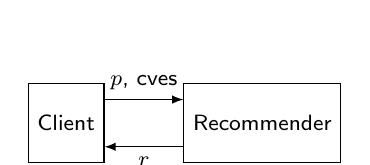
\begin{tikzpicture}[scale=1, every node/.style={scale=1}, node distance=1cm, font=\footnotesize\sffamily]
		\node[draw,minimum height=1cm] (client) at (0,0) {Client};
		\node[draw,minimum height=1cm,right=of client] (recommender) {Recommender};
		
		\draw[->] ([yshift=0.3cm]client.east) -- node[above] {$p$, cves} ([yshift=0.3cm]recommender.west);
		\draw[<-] ([yshift=-0.3cm]client.east) -- node[below] {$r$} ([yshift=-0.3cm]recommender.west);
	\end{tikzpicture}
	\caption{Vulnerability prioritization: a client requests recommendations for a set of CVEs, using client profile $p$}
	\label{fig:vuln-prio-scenario}
\end{figure}

\subsection{Isolated Execution}
\label{subsec:isolatedexecution}
In this paper we propose a mechanism to protect the privacy of client requests to the recommender.
This mechanism requires confidentiality of the data, requirements that can be satisfied using isolated execution. 
We use SGX enclaves~\cite{anati:2013,mckeen:2013,xing:2016,mckeen:2016} to create commodity trusted execution environments (TEEs) during operating system run-time.
We use TEEs to protect the privacy of client vulnerability profiles.
SGX enclaves rely on a trusted computing base of code and data loaded at enclave creation time, processor firmware, and processor hardware.
Program execution within an enclave is opaque to the underlying operating system and other mutually distrusting enclaves on the platform.
Enclaves operate in a dedicated memory area called the Enclave Page Cache, a range of dynamic random access memory that cannot be accessed by system software or peripherals~\cite{mckeen:2013}.
The CPU firmware and hardware are the root of trust of an enclave.
Isolation features implemented in firmware and hardware prevent access to the enclave's memory by the operating system and other enclaves.
While we use Intel SGX enclaves in our implementation of the privacy-preserving service, alternative commodity TEEs~\cite{mofrad:2017, brasser:2019} may be used.

\subsection{Threat Model}
\label{subsec:threat-model}

To construct a correct and relevant threat model in the scenario described above, we conducted in-depth interviews with software vendors and users that operate enterprise deployments.
Software vendors highlight the importance of protecting information about relevant software vulnerabilities during the pre- and post-disclosure phases, i.e. while assessing the vulnerability impact and prioritizing it, as well as before releasing a software patch (see Figure~\ref{fig:conf-window}).
We aim to protect the confidentiality of the vendor's software vulnerability priority ranking, since it reveals information about the severity of the vulnerability (as perceived by the vendor) and can be used to guide exploit development.
We assume clients have no information about unpublished vulnerabilities.
Hence, we must protect the confidentiality of the relevance and priority of the released security patches during the post-disclosure (denoted as $t_{pd}$) and post-patch (denoted as $t_{pp}$) phases, i.e. up to the point when software users patch their systems.
%===========================================================================
\begin{figure}[h]
  \centering
  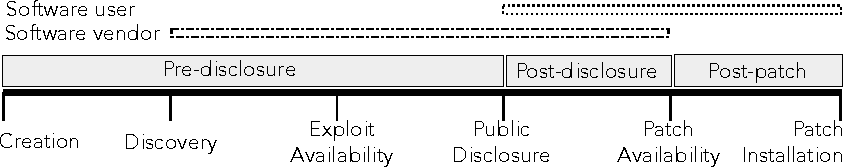
\includegraphics[width=\linewidth]{confidentiality-window}
  \caption{Vulnerability confidentiality window}
  \label{fig:conf-window}
\end{figure}
%===========================================================================

We assume the duration of the post-disclosure and post-patch phases is constant, equal to $T$:
\begin{equation}
    t_{pd} + t_{pp} = T
\end{equation}

The proposed architecture contains three main components - Client, Intermediary and Recommender.
We describe the security assumptions about the components of the proposed architecture.
\subsubsection*{Client}
The Client is potentially malicious, and may submit queries containing requests for arbitrary CVE identifiers.
The goal of the malicious Client is to reveal the privacy-preserving algorithm implemented in the Intermediary and distinguish the vulnerability profiles of other Clients from the vulnerability profiles generated by the Intermediary.
A set of Clients may collude to achieve this purpose.

\subsubsection*{Recommender}
The Recommender is an \textit{honest-but-curious} entity that aims to reveal the vulnerability profile of a specific Client.
The Recommender is assumed to have access to powerful computation capacity and is not sensitive to changes in the computation load of the queries received from the Client.
A collusion between the Client and the Recommender reveals the vulnerability profile of the colluding Client and is out of the scope of this model.

\subsubsection*{Intermediary}
The Intermediary is potentially malicious and aims to reveal the vulnerability profile of a specific Client.
A collusion between the Client and the Intermediary reveals the vulnerability profile of the colluding Client and is out of the scope of this model.
However, we consider that the isolated execution enclave that hosts the privacy protection mechanism is trustworthy;
its trustworthiness can be established through remote attestation by any of the components participating in the protocol.
Isolated execution enclaves used in the implementation of the Intermediary are vulnerable to side-channel attacks~\cite{wang:2017};
we explicitly exclude side-channel attacks from this threat model, since they can be mitigated through improved software implementation.

We consider a remote adversary with attack capabilities on the network and platform level.
The adversary is capable to observe and interact with the network communication between Client and the Recommender, as well with the communication among the internal services of the Recommender.
Furthermore, the adversary can launch arbitrary processes and obtain root access on the hosts running the Recommender.

\section{Vulnerability Profile Privacy}
\label{sec:solution}

As discussed in Section~\ref{subsec:threat-model} above, our goal is to protect the privacy of individual Client vulnerability profiles.
To design a solution for this task, we consider the following defining aspects: 
\textit{(i)} Client profile updates are sparse (e.g. one request every period $T$); 
\textit{(ii)} vulnerability profiles evolve after every period $T$;
\textit{(iii)} the value of an arbitrary snapshot of the vulnerability profile decays in time $T$, equal to the length of software user's confidentiality window.
These are aspects that are sound in the context of vulnerability prioritization, but may not hold for other recommender systems.

While a myriad of definitions, approaches and techniques have been proposed for privacy protection, it remains an elusive goal.
One reason is the discrepancy between the assumptions required for a solution to offer data privacy protection in the presence of other related data sets.
Another reason is the trade-off between data privacy and data utility present in most privacy-preserving solutions~\cite{dwork:2006, dwork:2014}.

To protect the privacy of Client vulnerability profiles, we design an approach based on a combination of k-anonymity~\cite{samarati:1998, samarati:2001} and local differential privacy~\cite{bassily:2017, tang:2017, zheng:2017}.
A combination of the two approaches guarantees that queries derived from Client vulnerability profiles are released only in large enough batches that contain additional queries derived from statistically different pseudo vulnerability profiles.
This approach prevents the direct release of information about subgroups and provides differential privacy guarantees by adding pseudo-random noise (in the form of fake queries) to the genuine queries based on individual Client vulnerability profiles.

This approach, adapted to the vulnerability recommender system described in~\cite{cobleigh:2018}, allows us to substitute the privacy-utility trade-off with a privacy-cost relation.
Intuitively, larger proportions of noise accompanying genuine queries lead to stronger privacy of the respective Client vulnerability profile.
While increasing computational cost of the recommender, this allows to proportionally decrease the utility of information observed by the adversary, without utility loss for the client.

\subsection{k-anonymous Vulnerability Profiles}
\label{subsec:solution-diff-privacy}
We next describe the mechanism for protecting the anonymity of queries derived from Client vulnerability profiles.
Our approach is based on two fundamental aspects: 
\textit{(1)} issuing queries in large enough batches, and 
\textit{(2)} mixing queries derived from genuine Client vulnerability profiles (called \textit{genuine queries)} with pseudo-random noise expressed as queries derived from statistically different pseudo vulnerability profiles (called \textit{pseudo queries}).

We next present the approach of issuing a single genuine query per batch.
Each Client vulnerability profile consists of exactly $n$ different properties, where each property describes the Client's preference for a certain aspect of a vulnerability.
Preferences are represented as a vector $p$ describing the Client profile, where each individual property is denoted $v_i$.
\begin{equation}
p = \{v_1, v_2, \ldots, v_n\}
\end{equation}

For example, a Client vulnerability profile may be built by ranking three different vulnerability properties: 
confidentiality impact, 
integrity impact, 
and availability impact.
A client preference could be that the Client considers that vulnerabilities affecting confidentiality have higher priority, while vulnerabilities with an impact on integrity or availability have lower priority.
A profile is then represented as: $\{0.9, 0.2, 0.2\}$, where a higher value $v_i$ implies that a property is considered more important.

To reduce the utility of information disclosed to the adversary through queries, the pseudo queries should fulfill two requirements:
\textit{(i)} introduce sufficient noise regardless of the cardinality of the profile $|p|$ and of the values of the elements $v_i$ in the profile;
\textit{(ii)} have the same dimensions and be indistinguishable from the genuine query.
Different from database anonymization approaches~\cite{samarati:1998, samarati:2001, holohan:2017}, low variability in the data set does not satisfy our privacy requirements, since it leaks Client vulnerability profile data.
Therefore we add a third condition that the pseudo queries must satisfy, along with conditions \textit{(i)}, \textit{(ii)} above:
\textit{(iii)} the query data set should display high variability (or high standard deviation in statistical terms).

Thus, on every period $T$, the Client submits a query $Q_g$ to the Intermediary.
The Intermediary derives $k - 1$ pseudo queries $Q_p$ that along with $Q_g$ are submitted to the Recommender.
The Recommender processes all of the queries and returns $k$ different responses based on the received queries.
As a result, neither the adversary observing the network, nor the potentially malicious Recommender are aware which of the $k$ (profile, response)-pairs belongs to the Client.
Upon receiving $k$ replies the Intermediary discards all pseudo queries $Q_p$ and returns to the Client the reply to query $Q_g$.
The variability of the $k$ profiles is sufficiently large to make it unfeasible to draw any conclusions about the contents of the genuine profile.
The size $k-1$ is configurable, depending on the computational cost acceptable for the Recommender and the privacy guarantees requested by the Client.

Having described the Client vulnerability profile anonymization principles, we next discuss the use of isolated execution to provide platform security guarantees of the Intermediary.


\subsection{Privacy Protection with Isolated Execution}
\label{subsec:solution-sgx}

The privacy-preserving mechanism described above can be implemented by any component of the proposed architecture: Client, Intermediary, or Recommender (see Section~\ref{subsec:threat-model}).
A straightforward client implementation is possible;
however, this places a large load on the client and generate excessive network traffic.
Alternatively, a client may choose to instead send only a single request to the intermediary.
The intermediary is then responsible for sending multiple requests to the Recommender.
From the Client's point of view, a \textit{trustworthy} intermediary allows to reduce external network traffic, since the intermediary can be placed close to the recommender system.
The privacy-preserving mechanism can also be implemented by the Recommender provider itself, thus reducing the network latency between the Intermediary and the Recommender to near zero.
However, this is incompatible with the honest-but-curious Recommender described in Section~\ref{subsec:threat-model}.

Trustworthy intermediary functionality can be implemented using the functionality of a TEE.
The TEE should support remote attestation, isolated execution, and sealing of sensitive data.
In the description below, a solution designed on Intel SGX is described, but we stress that alternative commodity TEEs may be used instead.
We consider a scenario with the following requirements:
\begin{itemize} 
	\item A malicious Intermediary or Recommender system should not be able to know if a certain client profile is the genuine client profile for a particular Client.
	\item The Client should be able to attest the integrity of the Intermediary before sending sensitive data.
	\item The Recommender should be oblivious to the privacy-preserving measures taken by the Intermediary: changes to the privacy preserving mechanism in the Intermediary should not require any modifications of the Recommender.
\end{itemize}

We propose a solution as depicted in Figure~\ref{fig:tee-privacy}.
The Client starts by attesting the integrity of the Intermediary through remote attestation.
During this stage, the Client receives proof that the TEE of the Intermediary has not been tampered with, and negotiates a shared secret $S$, which can be used to send encrypted data to the TEE.
The key $S$ is confined within the TEE and cannot be read from the outside.


\begin{figure}[h]
	\centering
	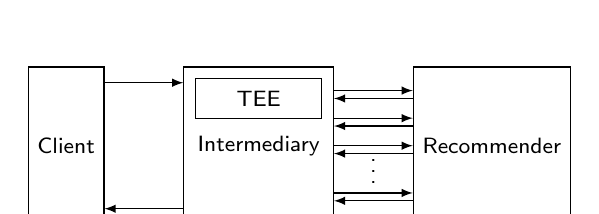
\begin{tikzpicture}[scale=1, every node/.style={scale=1}, node distance=1cm, font=\footnotesize\sffamily]
		\node[draw,minimum height=2cm] (client) at (0,0) {Client};
		\node[draw,minimum height=2cm,minimum width=1.9cm,right=of client] (intermediary) {Intermediary};
		\node[draw,minimum height=2cm,right=of intermediary] (recommender) {Recommender};
		
		\node[draw,minimum height=0.5cm,minimum width=1.6cm,below right] (tee) at ([xshift=0.15cm,yshift=-0.15cm]intermediary.north west) {TEE};
		
		\draw[->] ([yshift=0.8cm]client.east) -- ([yshift=0.8cm]intermediary.west);
		
		\draw[->] ([yshift=0.7cm]intermediary.east) -- ([yshift=0.7cm]recommender.west);
		\draw[<-] ([yshift=0.6cm]intermediary.east) -- ([yshift=0.6cm]recommender.west);
		
		\draw[->] ([yshift=0.35cm]intermediary.east) -- ([yshift=0.35cm]recommender.west);
		\draw[<-] ([yshift=0.25cm]intermediary.east) -- ([yshift=0.25cm]recommender.west);
		
		\draw[->] ([yshift=0.00cm]intermediary.east) -- ([yshift=0.00cm]recommender.west);
		\draw[<-] ([yshift=-0.1cm]intermediary.east) -- ([yshift=-0.1cm]recommender.west);

		\draw[->,above] ([yshift=-0.6cm]intermediary.east) -- node {$\vdots$} ([yshift=-0.6cm]recommender.west);
		\draw[<-] ([yshift=-0.7cm]intermediary.east) -- ([yshift=-0.7cm]recommender.west);
		
		\draw[<-] ([yshift=-0.8cm]client.east) -- ([yshift=-0.8cm]intermediary.west);
	\end{tikzpicture}
	\caption{Proposed design with an Intermediary running in a TEE}
	\label{fig:tee-privacy}
\end{figure}


Next, the Client either updates its client profile, or requests recommendations from the Recommender.
In both cases, the Client sends a single request to the Intermediary, encrypted with the shared secret $S$.
The TEE of the Intermediary can then decrypt the request.

For a request to update the profile, the TEE generates $k-1$ new pseudo profiles, to be used as described in Section~\ref{subsec:solution-diff-privacy}.

For a request for recommendations, the TEE looks up $k$ different profiles, of which only one is the genuine profile.
These profiles are then used to generate $k$ queries to the Recommender.
All $k$ responses are then returned to the Intermediary.
The Intermediary next sends all results into the TEE, which picks the result corresponding to the genuine client profile.
This result is encrypted with $S$ and sent back to the Client, where it can be decrypted.
This design achieves the following properties:
\begin{itemize}
	\item The decrypted data with the genuine client profile is never available alone to the Intermediary \emph{outside} the TEE. 
	Only the collection of $k$ profiles is available, and it is not possible to distinguish the genuine profile from pseudo profiles.
	\item Following the definition of a TEE, an entity on the outside can never read data inside the TEE.
	\item If the adversary modifies the TEE, the attestation phase will fail, and no sensitive data will be sent to the TEE.
	\item The Recommender remains unaware of the Intermediary and simply receives extra requests made with several different profiles.
\end{itemize}
Together, these properties fulfill the requirements described earlier in this section.
We will next describe implementation details in Section~\ref{sec:recsyssgx:implementation}.

\section{Implementation}
\label{sec:recsyssgx:implementation}

To evaluate our proposed design and demonstrate its viability, we implemented a proof-of-concept prototype.
The implementation uses Intel SGX to provide the TEE of the Intermediary, and was evaluated with hardware support for Intel SGX.

The implementation includes three major components: Client, Intermediary, and Recommender, (see Figure~\ref{fig:tee-privacy}).
In this implementation our focus is the Client and the Intermediary.
We assume that the Recommender is already implemented, but without any privacy-enabling technologies, as explained in Section~\ref{subsec:scenario} and \cite{cobleigh:2018}.
The three main features that the implementation must support are remote attestation, profile management, and recommendation generation.
We next describe their implementation details.

\subsection{Remote attestation}
\label{subsec:impl-remoteattestation}
The first step before the Client can trust the Intermediary is to attest the Intermediary's TEE, in this case an SGX enclave.
The remote attestation implementation uses the suggested design from Intel \cite{sgx-ra-example}, using a modified Sigma protocol to derive a shared secret in the attestation phase.

We next briefly describe the procedure (see  \cite{sgx-ra-example} for more details).
First, the Client starts the attestation process by contacting the Intermediary, which initiates the remote attestation process inside the enclave.
The Client proceeds by retrieving a signature revocation list from Intel Attestation Services (IAS), and sends this to the enclave together with other data.
The enclave proceeds by returning a quote, which can then be verified by the Client.
This verification is done by first contacting IAS, to verify that the quote is made by an enclave on trusted hardware.
After this, the hash value of the enclave's code can be read from the quote.
If this matches the expected value, the Client can be certain that the enclave has not been tampered with.

After this point, both the enclave and the Client has a shared secret $S$ that can be used to secure further communications.
Note that this secret is only available to the Client and the enclave, \emph{not} the Intermediary outside the enclave.

\subsection{Profile Management}
\label{subsec:impl-profilemanagement}


\begin{figure}[ht]
	\centering
	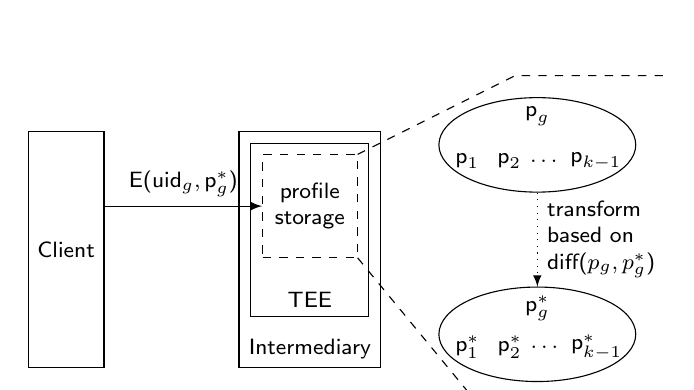
\begin{tikzpicture}[scale=1, every node/.style={scale=1}, node distance=1.7cm, font=\footnotesize\sffamily]
	\node[draw,minimum height=3.0cm] (client) at (0,0) {Client};
	\node[draw,minimum height=3.0cm,minimum width=1.8cm,right=of client] (intermediary) {};
	\node[draw,minimum height=2.2cm,minimum width=1.5cm,below right] (tee) at ([xshift=0.15cm,yshift=-0.15cm]intermediary.north west) {};
	\node[draw,dashed,minimum height=1.3cm,minimum width=1.2cm,below right,align=center] (teemgmt) at ([xshift=0.15cm,yshift=-0.15cm]tee.north west) {profile\\storage};

	\node[above] at (intermediary.south) {Intermediary};
	\node[above] at (tee.south) {TEE};

	\draw[->] (client.east |- teemgmt.west) -- node[above] {E($\text{uid}_g,\text{p}_g^{*}$)} (teemgmt.west);
	
	\node[draw,ellipse,minimum width=2.5cm,minimum height=1.2cm,below right=-0.25cm and 2cm of intermediary.north] (profbefore) {};
	\node[draw,ellipse,minimum width=2.5cm,minimum height=1.2cm,above right=0cm and 2cm of intermediary.south] (profafter) {};
	
	% profiles inside ellipses
	\node[below] (pc) at (profbefore.north) {$\text{p}_g$};
	\node[above] (p1) at (profbefore.south west) {$\text{p}_1$};
	\node[inner sep=0,right=0.1cm of p1] (p2) {$\text{p}_2$};
	\node[inner sep=0,right=0.1cm of p2] (pdots) {$\dots$};
	\node[inner sep=0,right=0.1cm of pdots] (pk) {$\text{p}_{k-1}$};

	\node[below] (pcs) at (profafter.north) {$\text{p}_g^{*}$};
	\node[above] (p1s) at (profafter.south west) {$\text{p}_1^{*}$};
	\node[inner sep=0,right=0.1cm of p1s] (p2s) {$\text{p}_2^{*}$};
	\node[inner sep=0,right=0.1cm of p2s] (pdotss) {$\dots$};
	\node[inner sep=0,right=0.1cm of pdotss] (pks) {$\text{p}_{k-1}^{*}$};

	% transition between old and new profiles
	\draw[->,dotted] (profbefore.south) -- node[right,align=left] (transformlabel) {transform\\based on\\diff($p_g,p_g^{*}$)} (profafter.north);

	% dashed lines surrounding ellipses
	\draw[dashed] (teemgmt.north east) -- +(2cm,1cm) node (topcrv) {} -- (topcrv -| transformlabel.east);
	\draw[dashed] (teemgmt.south east) -- +(1.4cm,-1.7cm) node (bottomcrv) {} -- (bottomcrv -| transformlabel.east);

	\end{tikzpicture}
	\caption{Enclave profile management during profile update}
	\label{fig:impl-profilemanagement}
\end{figure}

The profile management is located within the trusted enclave.
This ensures that its behavior can be verified by the Client, such that it does not leak information to an attacker.

Each client profile $p_i$, has a corresponding id $\text{uid}_i$, used in communication between the different entities.
Furthermore, for each \emph{genuine} client profile $p_g$, there are $k-1$ \emph{pseudo} profiles.
Using a different set of pseudo profiles for each genuine profile ensures that colluding clients cannot find pseudo profiles for other clients.
The profile management keeps a record over the mapping between genuine and pseudo profiles, such that the same set of pseudo profiles is used during profile update or recommendation generation for a specific genuine profile.

As the user's preferences change, the profile stored in the enclave needs to be updated.
An overview of this is shown in Figure~\ref{fig:impl-profilemanagement}.
During the profile update stage, the Client sends an encrypted updated genuine profile $p_g^*$ to the Intermediary.
The profile is decrypted inside the enclave, which then applies a transformation function as described below. 
The transformation is applied to each one of the $k-1$ pseudo profiles.
This ensures that an outside observer can only see that all profiles have been updated, but still cannot know which one that is the genuine profile.

There are two main events in the life cycle of pseudo profiles: the initial pseudo profile generation, and updates of the pseudo profile.
First, when a new genuine profile is created for the first time, $k-1$ new pseudo profiles must also be created.
Based on requirements listed in Section~\ref{subsec:solution-diff-privacy}, the pseudo profiles should be indistinguishable from a genuine profile.
To achieve this during initial pseudo profile generation, we select a profile such that its properties are distributed according the distribution of each property's value over all existing profiles, inspired by the work on $t$-closeness \cite{li:2007}.
This ensures that the newly generated pseudo profiles is non-distinguishable from genuine profiles.

Second, when a profile should be updated, following the terminology from Figure~\ref{fig:impl-profilemanagement}, we want to implement a $\texttt{diff()}$ function that updates the pseudo profiles based on the update of the genuine profile.
This function should:
\textit{(i)} hide \emph{which} property of the profile that was updated, and
\textit{(ii)} hide the exact \emph{value difference} between the new and the old property.
Without loss of generality, we can assume that during update of a genuine profile $p_g$ to its new value $p_g^*$, only a single property $v_i$ of the profile is modified\footnote{A single profile update modifying multiple properties can be converted to several consecutive updates, each modifying a single property.}.

To hide which property $v_i$ that is updated, for every pseudo profile, we randomly select a property $v_j$ from that profile ($1 \le j \le n$), whose value is updated.
The result is that different properties are updated, and since an outside observer does not know the genuine profile, it is not possible to find out which actual property that was updated.

To hide the exact value difference between the old property $v_i$ and the new property $v_i^*$, we suggest a solution similar to differential privacy \cite{dwork:2006}.
While the genuine profile is updated to (the exact) new property value $v_i^*$, noise is added to the pseudo profile.
The noise is based on the difference $v_i - v_i^*$, such that the exact value of the difference is hidden.
The distribution from which to draw the noise may be varied, in our proof-of-concept we base it on the Laplace distribution commonly used in $\epsilon$-differential privacy.

\subsection{Recommendation Generation}
\label{subsec:impl-recgen}

\begin{figure}[ht]
	\centering
	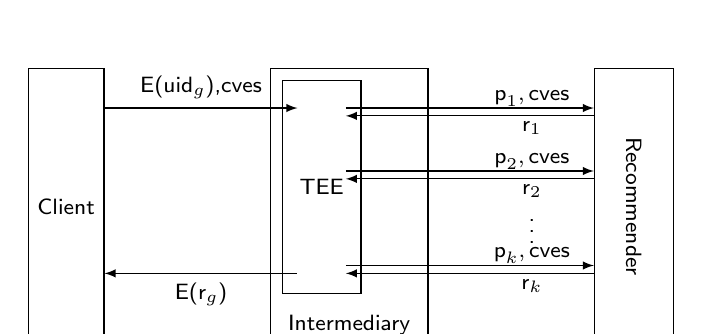
\begin{tikzpicture}[scale=1, every node/.style={scale=1}, node distance=2.1cm, font=\footnotesize\sffamily]
		\node[draw,minimum height=3.5cm] (client) at (0,0) {Client};
		\node[draw,minimum height=3.5cm,minimum width=2cm,right=of client] (intermediary) {};
		\node[draw,minimum height=3.5cm,minimum width=1cm,right=of intermediary] (recommender) {};
		
		\node[above] at (intermediary.south) {Intermediary};
		\node[rotate=-90] at (recommender.center) {Recommender};
		
		\node[draw,minimum height=2.7cm,minimum width=1cm,below right] (tee) at ([xshift=0.15cm,yshift=-0.15cm]intermediary.north west) {TEE};
		
		\coordinate (clientreq) at ([yshift=1.0cm,xshift=0.2cm]tee.west);
		\coordinate (clientres) at ([yshift=-1.1cm,xshift=0.2cm]tee.west);
		\draw[->] (client.east |- clientreq) -- node[above] {E($\text{uid}_g$),cves} (clientreq);
		
		\coordinate (r1) at ([yshift=1.0cm,xshift=-0.2cm]tee.east);
		\coordinate (r1r) at ([yshift=0.9cm,xshift=-0.2cm]tee.east);
		\coordinate (r2) at ([yshift=0.2cm,xshift=-0.2cm]tee.east);
		\coordinate (r2r) at ([yshift=0.1cm,xshift=-0.2cm]tee.east);
		\coordinate (rk) at ([yshift=-1.0cm,xshift=-0.2cm]tee.east);
		\coordinate (rkr) at ([yshift=-1.1cm,xshift=-0.2cm]tee.east);
		
		\draw[->] (r1) -- node[above=-0.1cm,near end] {$\text{p}_1, \text{cves}$} (r1 -| recommender.west);
		\draw[<-] (r1r) -- node[below=-0.05cm,near end] {$\text{r}_1$} (r1r -| recommender.west);

		\draw[->] (r2) -- node[above=-0.1cm,near end] {$\text{p}_2, \text{cves}$} (r2 -| recommender.west);
		\draw[<-] (r2r) -- node[below=-0.05cm,near end] (r2rnode) {$\text{r}_2$} (r2r -| recommender.west);

		\draw[->] (rk) -- node[above=-0.1cm,near end] (rknode) {$\text{p}_k, \text{cves}$} (rk -| recommender.west);
		\draw[<-] (rkr) -- node[below=-0.05cm,near end] {$\text{r}_k$} (rkr -| recommender.west);
		
		\node[] at ($(r2rnode)!0.5!(rknode)$) {\vdots};
		
		\draw[<-] (client.east |- clientres) -- node[below] {E($\text{r}_g$)} (clientres);
	\end{tikzpicture}
	\caption{Recommendation generation}
	\label{fig:impl-recgen}
\end{figure}

We illustrate the flow for recommendation generation in Figure~\ref{fig:impl-recgen}.
When the Client wishes to request recommendations, it sends a request to the Intermediary.
The request contains an encrypted id ($\text{uid}_g$), and a list of CVEs to rank.
The enclave decrypts the id, and returns $k$ different profiles to the Intermediary, outside of the enclave.
One of these profiles is the genuine client profile ($\text{p}_g$), but to the outside observer, all profiles are indistinguishable.

For each of the $k$ profiles, the Intermediary sends one request to the Recommender, which returns $k$ different responses.
The responses are forwarded to the enclave which selects only response $\text{r}_g$ corresponding to the genuine user profile $p_g$, encrypts it, and returns it to the Client.

An implementation must consider several aspects to avoid leaking information.
First, the order of profiles must be randomized, such that the position of the genuine profile is not known.
Second, even though the id and response is encrypted, the size of the ciphertext may still leak information, if different user profiles and responses from the Recommender have different sizes.
It is therefore important for the enclave to ensure that all ids have identical size, as well as verifying that responses from the Recommender do not differ in size.
In practice, this does not limit the functionality of the system: both the id and recommender response can be padded inside the enclave to ensure equal size.
Note that since it is the communication between client and enclave that is padded, the Recommender does not have to be modified.

\section{Evaluation}
\label{sec:recsyssgx:evaluation}
To evaluate the performance overhead of the proposed privacy-enabling mechanism, we measured the response time for recommendation generation.

Consider the setup in Figure~\ref{fig:tee-privacy}, with each entity running on a different host, connected to the same local network.
The Recommender is an actual implementation of a recommender as described in \cite{cobleigh:2018}, and the Intermediary's TEE is on a CPU with hardware support for Intel SGX.
We performed the following measurements.
First, three random sets of CVEs were constructed, containing 30, 100, and 1000 different CVEs, respectively.
Second, for each such set, we perform a test without the Intermediary as a baseline; 
in this test the Client connects directly to the Recommender, without any privacy protection.
This can be used as a reference when comparing to the other measurements.
Third, again for each set of CVEs, we performed five tests with different privacy levels, i.e. different values of $k$.
Recall that $k$ determines the number of profiles that are sent to the Recommender, so for e.g. $k=8$, there is one genuine and seven pseudo profiles being sent to the Recommender.
Each test was repeated 100 times, and the resulting mean, median, and standard deviation are presented in Table~\ref{tbl:evaluation}.
Note that the baseline measurement, in which the Client connects directly to the Recommender, is denoted by $k$ set to \emph{none}.



\begin{table}[ht]
    \centering
    \caption{Response times for recommendation generation for various number of CVEs and various values of $k$}
    \begin{tabular}{rrrrr}
        \toprule
        \#CVEs & $k$ & Mean (ms) & Median (ms) & St.dev (ms) \\
        \midrule
        30 & \emph{none} &   94.2 &   93.8 &   3.2 \\
           & 1           &  106.7 &  106.4 &   7.2 \\
           & 8           &  324.0 &  323.0 &  21.1 \\
           & 16          &  589.3 &  583.4 &  21.0 \\
           & 32          & 1117.6 & 1114.5 &  31.1 \\
           & 64          & 2154.7 & 2159.6 &  32.6 \\
        \midrule
        100 & \emph{none} &  122.0 &  121.6 &    2.6 \\
            & 1           &  135.2 &  135.0 &    2.5 \\
            & 8           &  378.0 &  371.7 &   33.0 \\
            & 16          &  662.5 &  650.5 &   39.9 \\
            & 32          & 1206.7 & 1198.0 &   49.9 \\
            & 64          & 2281.7 & 2277.3 &   44.0 \\
        \midrule
        1000 & \emph{none} &  442.6 &  441.6 &    5.5 \\
             & 1           &  463.6 &  462.9 &    6.5 \\
             & 8           &  813.4 &  777.5 &  108.6 \\
             & 16          & 1536.7 & 1502.8 &  153.1 \\
             & 32          & 2682.3 & 2661.1 &  136.1 \\
             & 64          & 4881.5 & 4836.1 &  154.9 \\
        \bottomrule
    \end{tabular}
    \label{tbl:evaluation}
\end{table}

The evaluation of the prototype implementation highlights the relation between the privacy guarantees and the response time of the recommender system.
Requests to recommender systems for vulnerability prioritization are expected to be sparse and potentially asynchronous.
Therefore, we consider the increase in response time detailed in Table~\ref{tbl:evaluation}  acceptable, considering the added benefit of data privacy.

\section{Related Work}
\label{sec:related}
In this paper we address the challenge of protecting the privacy of Client profiles in a vulnerability recommender service.
While this topic was not addressed earlier, we base our approach on a rich body of privacy and anonymity research.
We next review the related work.

\subsection{Privacy for Recommender Systems}
\label{subsec:related-privacy}

McSherry et al. described the design and implementation of a platform for privacy-preserving data analysis for SQL-like queries~\cite{mcsherry:2009}.
While this approach allows to write applications that provide privacy guarantees in an \textit{honest-but-curious} threat model, it is not backward-compatible with existing applications and requires native implementations in the Privacy Integrated Queries platform. Abadi et al. described algorithmic techniques for learning and a refined analysis of privacy costs within the framework of differential privacy~\cite{abadi:2016}.
The approach is geared towards training deep neural networks with non-convex objectives.
The solution enables this functionality under a modest privacy budget and at a manageable cost in software complexity and model quality.
However, the approach is not suitable for the \textit{honest-but-curious} threat model, since it relies on a trustworthy implementation of the framework on the data processing end.
Our approach introduces a privacy-protection layer that is independent of the implementation of the data processing (in this case a recommender system) and can therefore be applied to a wide range of applications.

Ohrimenko et al. described an approach for oblivious multi-party machine learning on trusted processors~\cite{ohrimenko:2016}.
The approach relies of a set of custom machine learning algorithms for trusted processors that make use of general-purpose oblivious primitives.
For further security, the multi-party machine learning mechanism is implemented in trusted execution environments (namely Intel SGX enclaves).
The Prochlo~\cite{bittau:2017} implementation likewise uses Intel SGX enclaves to implement the Encode, Shuffle, Analyze architecture for privacy-preserving software monitoring.
The architecture is tailored for anonymizing data streams from many heterogeneous sources and allows to expose anonymized data to third parties.
In this paper, we similarly rely on SGX enclaves to create trusted execution environments to run an implementation for query anonymization.
We address a different use case, where the privacy of a single profile using the recommender system is preserved against an adversary capable to observe the queries and the internals of the recommender system.

\subsection{Vulnerability Selection}
\label{subsec:related-selection}

Vulnerability \textit{detection} precedes and is closely related to vulnerability \textit{selection}.
In~\cite{shoshitaishvili:2017} the authors address the challenge of shifting vulnerability detection from a human-centric to a computer-centric approach.
In particular, the paper presents a design and implementation for a human-assisted automated
vulnerability analysis system.
VULCON (VULnerability CONtrol) is a vulnerability management strategy described in~\cite{farris:2018}. 
It is based on two metrics, namely time-to-vulnerability remediation and  total vulnerability exposure.
Based on inputs such as  vulnerability scan reports, metadata about the discovered vulnerabilities, asset criticality, and personnel resources VULCON prioritizes vulnerabilities for patching.
Both vulnerability \textit{detection} and vulnerability \textit{selection} may require anonymity and privacy guarantees for the Client profiles in privacy-sensitive settings.
Our work addresses this by describing a privacy protection mechanism for Client vulnerability profiles.

\section{Conclusion}
\label{sec:recsyssgx:conclusion}

Automated vulnerability prioritization and patch selection become increasingly necessary in order to cope with the growing complexity of corporate software environments.
Earlier research on recommender systems for vulnerability prioritization and patch selection did not address the privacy of client vulnerability profiles.
In this work we presented a privacy-preserving mechanism that helps protect client vulnerability profiles in the context of recommender systems for vulnerability prioritization and patch selection;
to the best of our knowledge, this is the first work addressing this aspect. 
We implement a prototype of the proposed solution using Intel SGX enclaves and a functioning recommender system for vulnerability prioritization and patch selection.
Our evaluation of the prototype implementation reveals that the response time increases along with the proportion of pseudo queries issues with each request, but remains acceptable considering that requests are expected to be sparse.
The evaluation result highlights that the proposed mechanism is practical and can complement existing recommender systems for vulnerability prioritization and patch selection.
 

\section*{Acknowledgment}
This work was financially supported by the Swedish Foundation for Strategic Research, grant RIT17-0035.

%\bibliographystyle{IEEEtran}
%\bibliography{sample-base}

%\end{document}

{\raggedright
	\printbibliography[segment=\therefsegment,heading=subbibliography]
}

}

\fi

\ifpaperVI
\newrefsegment
\addtolength{\apa}{2cm}
\fancyhead[RE]{\truncate{.95\headwidth}{\paperref{ch:slightlygreedy}: \paperVItitle}}
\chapter[\paperVItitle]{\texorpdfstring{%
		\paperVItitle}{%
		\paperVItitle}}
\label{ch:slightlygreedy}
\paperRemark{\paperVIref} % TODO: consider adding e.g. Reformatted for clarity

{

%\documentclass{acm_proc_article-sp}
%\documentclass{llncs}
%\documentclass[a4paper,twoside]{article}

%\usepackage[T1]{fontenc}
%\usepackage{multirow}
%\usepackage{rotating}
%\usepackage{tikz}
%\usetikzlibrary{arrows,backgrounds,patterns,shapes,decorations.markings,decorations.pathreplacing,positioning,matrix}
%\usepackage{enumitem}
%\usepackage{hyperref}
%\hypersetup{pdfborder=0 0 0}
%\usepackage{listings}
%\usepackage{booktabs}
%\usepackage{array}
%\usepackage{amsmath}
%\usepackage{amssymb}
%\usepackage{bm}
%\usepackage{calc}
%\usepackage{subcaption}
%\usepackage{multicol}

\newcommand{\cfor}{\textbf{for}}
\newcommand{\creturn}{\textbf{return}}
\newcommand{\cif}{\textbf{if}}
\newcommand{\celse}{\textbf{else}}
\newcommand{\cwhile}{\textbf{while}}
\newcommand{\crepeat}{\textbf{repeat}}

\newcounter{algcount}
\renewcommand{\thealgcount}{\arabic{algcount}}

\newcommand{\alg}[4]{
	\begin{table}[htbp]
		\centering
		\begin{tabular}{l}
			\toprule[0.4mm]
			\parbox{0.9\linewidth}{
				\refstepcounter{algcount}
				\label{#2}
				\parbox[t]{\widthof{\textbf{Algorithm \thealgcount}~--~}}{\textbf{Algorithm~\thealgcount}~--~}
				\parbox[t]{0.9\linewidth - \widthof{\textbf{Algorithm \thealgcount}~--~}}{{#1}}\vspace{.65mm}
			}\\
			\midrule[0.4mm]
			\parbox{0.9\linewidth}{#3}\\
			\midrule
			\parbox{0.9\linewidth}{{#4}}\\
			\bottomrule[0.4mm]
		\end{tabular}
	\end{table}
}

\newcommand{\algref}[1]{{Algorithm \ref{alg:#1}}}

\renewcommand{\sectionautorefname}{Section}
\renewcommand{\subsectionautorefname}{\sectionautorefname}

%\subfigtopskip=0pt
%\subfigcapskip=0pt
%\subfigbottomskip=0pt

%\begin{document}

%\title{Not so Greedy: Enhanced Subset Exploration for Nonrandomness Detectors}

%\author{Linus Karlsson \and Martin Hell \and Paul Stankovski}

% Linus Karlsson ORCID: https://orcid.org/0000-0002-6332-5078

%\institute{Dept. of Electrical and Information Technology, Lund University,\\
%P.O. Box 118, 221 00 Lund, Sweden\\
%\email{\{linus.karlsson,martin.hell,paul.stankovski\}@eit.lth.se}
%}

%\maketitle

\section*{Abstract}
Distinguishers and nonrandomness detectors are used to distinguish ciphertext from random data. In this paper, we focus on the construction of such devices using the maximum degree monomial test. This requires the selection of certain subsets of key and IV-bits of the cipher, and since this selection to a great extent affects the final outcome, it is important to make a good selection. We present a new, generic and tunable algorithm to find such subsets. Our algorithm works on any stream cipher, and can easily be tuned to the desired computational complexity. We test our algorithm with both different input parameters and different ciphers, namely Grain-128a, Kreyvium and Grain-128. Compared to a previous greedy approach, our algorithm consistently provides better results.

\section{Introduction}

Stream ciphers are symmetric cryptographic primitives which generate a pseudo-random sequence of digits, called the keystream, which is then combined with the plaintext message to produce a ciphertext. To generate the keystream, a public initialization vector (IV) and a secret key are used. It is important that an attacker cannot use the public IV to deduce information about the keystream, since this would put the encrypted message at risk.

To prevent such an attack, the key and IV are mixed during an initialization phase, before the stream cipher produces actual keystream. This initialization phase consist of a set of initialization rounds, during which the output of the cipher is suppressed.

A cipher needs to have an adequate amount of initialization rounds. Too many, and the cipher will have poor initialization performance, too few and an attacker may be able to perform an attack, e.g., a chosen-IV attack.

In this paper we will look into the design of distinguishers and nonrandomness detectors to perform cryptanalysis of different ciphers. The goal of such devices is to look at data and then determine whether the data is random data, or data from a specific cipher. Recall that for a good cipher, the keystream should be pseudo-random, so it should be hard to construct such a detection device, since data from a cipher should appear random to an outside observer.

Distinguishers and nonrandomness detectors differs in what degree of control an attacker has over the input. In a distinguisher, the key is fixed and unknown to the attacker, only the IV can be modified. In a nonrandomness detector, an attacker has more control, and can modify both key and IV bits.

The design of distinguishers and nonrandomness detectors has previously been discussed in the literature. Previous work such as \cite{englund:2007} has considered the design of such devices by using a test called the Maximum Degree Monomial (MDM) test. This test looks at statistical properties of a cipher to find weaknesses.

This test requires selection of a subset of the cipher's key and IV bits, which can be selected using, for example, a greedy algorithm, as described in ~\cite{stankovski:2010}.

We build upon this previous work and propose an improved, generalized, algorithm which outperforms the greedy algorithm in finding suitable subsets. We also implement and test our algorithm, and present new results on the stream ciphers Grain-128, Grain-128a and Kreyvium.

This paper is an extended and revised version of \cite{karlsson:2017}.
The major novelties are analysis of one more cipher (Kreyvium), a new test which investigates the effect of optimal starting subsets, and a more detailed descriptions of our algorithm.

The paper is organized as follows. In \autoref{sec:slightlygreedy:background} we present some required background, which is then used when describing our new algorithm in \autoref{sec:improvedalg}. Results are presented in \autoref{sec:results}, which is then followed by a discussion of related work in \autoref{sec:slightlygreedy:relatedwork}. \autoref{sec:slightlygreedy:conclusions} concludes the paper.

\section{Background} \label{sec:slightlygreedy:background}
In this paper we will mainly focus on the analysis of the two stream ciphers Grain-128a and Kreyvium. This selection of ciphers has been made since they share some interesting properties. They are both based on ciphers from the final eSTREAM portfolio (Grain~v1 and Trivium, respectively), but modified to have 128-bit keys. Both ciphers also update their internal state relatively slowly---a small fraction of the internal state is modified in each clock cycle. This requires both ciphers to have many initializations rounds.

For completeness, we start with a brief description of these two ciphers.
After this, in the rest of this chapter, we discuss the Maximum Degree Monomial test in more detail.

\subsection{Grain-128a}
The Grain-family of ciphers consist of a progression of multiple ciphers, starting with Grain~v1 \cite{hell:2006a}, which is included in the final eSTREAM portfolio of ciphers. This was extended into a 128-bit key version as Grain-128 \cite{hell:2006b}, and finally to the current version Grain-128a \cite{agren:2011}.

Grain-128a is a stream cipher with a 128 bit key and a 96 bit IV. It support two modes of operations, with or without authentication. For brevity, the following description will focus on the non-authenticated mode. Refer to the original paper for an extended description. The cipher is constructed with three major parts: one LFSR of size 128, one NFSR of size 128, and one pre-output function $h$ combining values from the LFSR and the NFSR. An overview of the cipher can be seen in \autoref{fig:grain128a}.

\begin{figure}
	\centering
	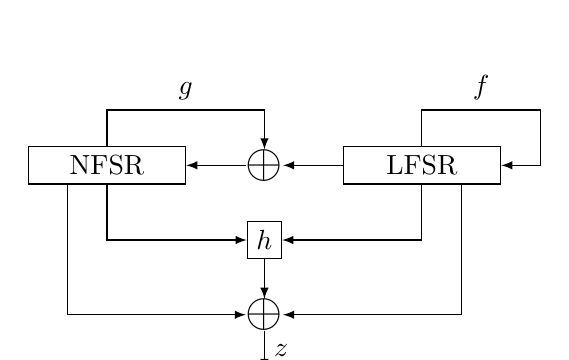
\begin{tikzpicture}[scale=1.0, every node/.style={scale=1.0}, node distance=2cm]
		\node[draw,minimum width=2cm] (nfsr) at (0,0) {NFSR};
		\node[right of=nfsr,inner sep=0,outer sep=0] (nfsrlfsrplus) {\LARGE $\oplus$};
		\node[draw,minimum width=2cm,right of=nfsrlfsrplus] (lfsr) {LFSR};
		
		\node[draw,below=0.5cm of nfsrlfsrplus] (h) {$h$};
		\node[below=0.5cm of h,inner sep=0,outer sep=0] (hplus) {\LARGE $\oplus$};
		
		\draw[->] (lfsr.west) -- (nfsrlfsrplus.east);
		\draw[->] (nfsrlfsrplus.west) -- (nfsr.east);
		
		\draw[->] (nfsr.south) |- (h.west);
		\draw[->] (lfsr.south) |- (h.east);
		
		\coordinate (nfsrsouth2) at ([xshift=-0.5cm]nfsr.south);
		\coordinate (lfsrsouth2) at ([xshift=0.5cm]lfsr.south);
		\draw[->] (nfsrsouth2) |- (hplus.west);
		\draw[->] (lfsrsouth2) |- (hplus.east);
		\draw[->] (h.south) -- (hplus.north);
		\draw[->] (hplus.south) -- ++(0cm,-0.5cm) node[midway,right] {$z$};
		
		% feedback functions.
		\coordinate[above=0.5cm of nfsrlfsrplus] (aboveplus);
		\draw[->] (nfsr.north) -- (aboveplus -| nfsr.north) -- (aboveplus) node[midway,above] {$g$} --  (nfsrlfsrplus.north);

		\coordinate[right=0.5cm of lfsr.east] (lfsrr);
		\draw[->] (lfsr.north) -- (aboveplus -| lfsr.north) -- (aboveplus -| lfsrr) node[midway,above] {$f$} -- (lfsrr) -- (lfsr.east);
	\end{tikzpicture}
	\caption{Overview of Grain-128a}
	\label{fig:grain128a}
\end{figure}

The functions $f(x)$ and $g(x)$ are the feedback functions for the LFSR and the NFSR respectively. They are defined as follows:
\[
f(x) = 1 + x^{32} + x^{47} + x^{58} + x^{90} + x^{121} + x^{128}
\]
and
\begin{align*}
	g(x) &= 1 + x^{32} + x^{37} + x^{72} + x^{102} + x^{128} + x^{44}x^{60} + x^{61}x^{125} + x^{63}x^{67} \\
		 &+ x^{69}x^{101} + x^{80}x^{88} + x^{110}x^{111} + x^{115}x^{117} + x^{46}x^{50}x^{58} \\
		 &+ x^{103}x^{104}x^{106} + x^{33}x^{35}x^{36}x^{40}
\end{align*}

The function $h(x)$ is defined as follows, where $s_i$ and $b_i$ correspond to the $i$th state variable of the LFSR and the NFSR respectively: 
\[
h = b_{12}s_{8} + s_{13}s_{20} + b_{95}s_{42} + s_{60}s_{79} + b_{12}b_{95}s_{94}
\]
Finally, the output $z$ from the cipher is constructed as:
\[
z = h + s_{93} + b_{2} + b_{15} + b_{36} + b_{45} + b_{64} + b_{73} + b_{89}
\]

The initialization of the cipher is as follows. At first the NFSR is filled with the 128 key bits, and then the LFSR is filled with the 96 IV-bits. The remaining 32 bits of the LFSR are filled with ones, except the final bit which is set to zero. After this, the cipher is clocked 256 times, during which the output is suppressed and instead fed back and XORed with the input to both the NFSR and LFSR. After this, the cipher is ready and starts to produce keystream.

\subsection{Kreyvium}
Kreyvium \cite{canteaut:2016} is based on another eSTREAM finalist, namely Trivium \cite{canniere:2006}. Trivium is notable for its simplistic design. It has an 80 bit key and an 80 bit IV. The authors of Kreyvium modifies the construction by increasing this to 128 bit for both the key and the IV.

Kreyvium's internal state consists of five different registers, of sizes 93, 84, 111, 128, and 128 bits. In the following brief description, we will call them $a$, $b$, $c$, $IV^*$, and $K^*$, respectively. The first three registers are the same as in Trivium, while the latter two are added in Kreyvium. An overview of the cipher can be found in \autoref{fig:kreyvium}.

\begin{figure}
	\centering
	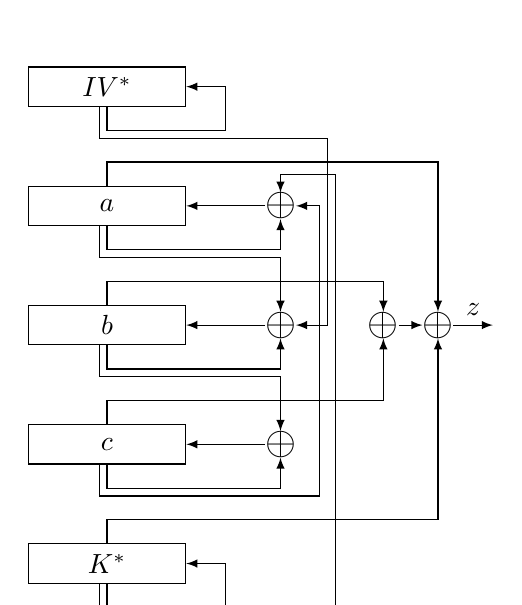
\begin{tikzpicture}[scale=1.0, every node/.style={scale=1.0}, node distance=1cm]
		\node[draw,minimum width=2cm,minimum height=0.5cm] (ivstar) at (0,0) {$IV^*$};
		\node[draw,minimum width=2cm,minimum height=0.5cm,below=of ivstar] (a) {$a$};
		\node[draw,minimum width=2cm,minimum height=0.5cm,below=of a] (b) {$b$};
		\node[draw,minimum width=2cm,minimum height=0.5cm,below=of b] (c) {$c$};
		\node[draw,minimum width=2cm,minimum height=0.5cm,below=of c] (kstar) {$K^*$};
		
		\node[right=3cm of b,outer sep=0,inner sep=0] (zplus) {\Large $\oplus$};
		\node[left=0.3cm of zplus,outer sep=0,inner sep=0] (zplusl) {\Large $\oplus$};
		\node[right=1cm of a,outer sep=0,inner sep=0] (aplus) {\Large $\oplus$};
		\node[right=1cm of b,outer sep=0,inner sep=0] (bplus) {\Large $\oplus$};
		\node[right=1cm of c,outer sep=0,inner sep=0] (cplus) {\Large $\oplus$};
		
		\coordinate[right=0.3cm of aplus] (aplusr);
		\coordinate[above right=0.4cm and 0.2cm of aplusr] (aplusr2);
		\coordinate[right=0.4cm of bplus] (bplusr);
		
		% z generation
		\draw[->] (zplus.east) -- ++(0.5cm,0) node[midway,above] {$z$};
		\draw[->] (zplusl.east) -- (zplus.west);
		
		\coordinate[above=0.3cm of a] (aabove);
		\coordinate[above=0.3cm of b] (babove);
		\coordinate[above=0.3cm of c] (cabove);
		\coordinate[above=0.3cm of kstar] (kstarabove);
		\draw[->] (a.north) -- (aabove) -- (aabove -| zplus.north) -- (zplus.north);
		\draw[->] (b.north) -- (babove) -- (babove -| zplusl.north) -- (zplusl.north);
		\draw[->] (c.north) -- (cabove) -- (cabove -| zplusl.south) -- (zplusl.south);
		\draw[->] (kstar.north) -- (kstarabove) -- (kstarabove -| zplus.south) -- (zplus.south);
		
		% various helpers.
		\coordinate[below=0.3cm of a] (abelow);
		
		% feedback for K*
		\coordinate[right=0.5cm of kstar] (kstarr);
		\coordinate[below=0.3cm of kstar] (kstarbelow);
		\draw[->] (kstar.south -| kstarbelow) -- (kstarbelow) -- (kstarbelow -| kstarr) |- (kstar.east);

		% feedback for IV*
		\coordinate[below=0.3cm of ivstar] (ivstarbelow);
		\coordinate[right=0.5cm of ivstar] (ivstarr);
		\draw[->] (ivstar.south -| ivstarbelow) -- (ivstarbelow) -- (ivstarbelow -| ivstarr) |- (ivstar.east);

		% feedback for b
		\draw[->] (bplus) -- (b.east);
		
		\coordinate[below left=0.1cm and 0.1cm of ivstarbelow] (ivstarbelow2);
		\coordinate[below left=0.1cm and 0.1cm of abelow] (abelow2);
		\coordinate[below=0.3cm of b] (bbelow);
		\draw[->] (a.south -| abelow2) -- (abelow2) -- (abelow2 -| bplus.north) -- (bplus.north);
		\draw[->] (b.south) -- (bbelow) -- (bbelow -| bplus.south) -- (bplus.south);
		\draw[->] (ivstar.south -| ivstarbelow2) -- (ivstarbelow2) -- (ivstarbelow2 -| bplusr) -- (bplusr) -- (bplus.east);
		
		% feedback for c
		\draw[->] (cplus) -- (c.east);
		
		\coordinate[below left=0.1cm and 0.1cm of bbelow] (bbelow2);
		\coordinate[below=0.3cm of c] (cbelow);
		\draw[->] (b.south -| bbelow2) -- (bbelow2) -- (bbelow2 -| cplus.north) -- (cplus.north);
		\draw[->] (c.south -| cbelow) -- (cbelow) -- (cbelow -| cplus.south) -- (cplus.south);
		
		% feedback for a
		\draw[->] (aplus) -- (a.east);
		
		\coordinate[below left=0.1cm and 0.1cm of cbelow] (cbelow2);
		\coordinate[below left=0.1cm and 0.1cm of kstarbelow] (kstarbelow2);
		\draw[->] (a.south -| abelow) -- (abelow) -- (abelow -| aplus.south) -- (aplus.south);
		\draw[->] (c.south -| cbelow2) -- (cbelow2) -- (cbelow2 -| aplusr) -- (aplusr) -- (aplus.east);
		\draw[->] (kstar.south -| kstarbelow2) -- (kstarbelow2) -| (aplusr2) -| (aplus.north);
	\end{tikzpicture}
	\caption{Overview of Kreyvium}
	\label{fig:kreyvium}
\end{figure}

Following the notation of the original paper, the registers $a$, $b$, and $c$ are numbered $s_1, \ldots, s_{93}$, followed by  $s_{94}, \ldots, s_{177}$, and finally $s_{178}, \ldots, s_{288}$, respectively. Then the output $z$ can be expressed as:

\[
z = s_{66} + s_{93} + s_{162} + s_{177} + s_{243} + s_{288} + K^*_0
\]

For every clock, each LFSR is shifted one step, and the following values are shifted in for each register:
\begin{align*}
s_1 &= s_{243} + s_{288} + K^*_0 + s_{286}s_{287} + s_{69} \\
s_{94} &= s_{66} + s_{93} + s_{91}s_{92} + s_{171} + IV^*_0 \\
s_{178} &= s_{162} + s_{177} + s_{175}s_{176} + s_{264} \\
K^*_{127} &= K^*_0 \\
IV^*_{127} &= IV^*_0 \\
\end{align*}

The initialization of the ciphers is as follows. The $a$ register is initialized with the first 93 key bits. The $b$ register is intialized with the first 84 IV bits. The $c$ register is initialized with the remaining IV bits, followed by all ones, except the final bit which is a zero. The $K^*$ register is filled with the key, and the $IV^*$ register is filled with the IV. After this the cipher is clocked 1152 times, during which the output is suppressed. After this, the cipher starts generating keystream.

\subsection{Maximum Degree Monomial Test}
The maximum degree monomial test was first presented in \cite{englund:2007} and described a clean way to detect nonrandomness by looking at the cipher output.

Considering an arbitrary stream cipher, we can consider it as a black box with two inputs, and one output. The input is the key $K$ and the initialization vector (IV) $V$ respectively, while the output is the generated keystream. We consider the concatenation of the key $K$ and the IV $V$ as a boolean space $B$ of dimension $b=|K| + |V|$.

Any Boolean function $g$ over a boolean space $B$ can be described by its Algebraic Normal Form (ANF)
\[
g(x_1, x_2, \ldots, x_b) = c_0 + c_1 x_1 + c_2 x_2 + \ldots + c_m x_1 x_2 \ldots x_b
\]
where the coefficients $c_i$ are either 0 or 1, thus describing if the term is included in the ANF or not. For the function $g$ above, the last term with coefficient $c_m$ describes the maximum degree monomial. If $c_m$ is zero, we say that the maximum degree monomial does not exist, while if $c_m$ is 1, we say it does exist. We note that for a randomly chosen Boolean function $g$, we would expect the maximum degree monomial to appear with a probability of $\frac{1}{2}$.

We are interested in finding out whether or not the maximum degree monomial exists in the ANF of the Boolean function of the first keystream bit. The rationale behind this is that intuitively, the maximum degree monomial tells us something about the mixing of the input to the cipher. Since the maximum degree monomial is the product of all inputs of the Boolean function, we expect to see it only if all inputs have been mixed.

It is well known that according to the Reed-Muller transform, the coefficient of the maximum degree monomial can be found simply by XORing all the entries in the truth table of a Boolean function as
\begin{align}
\bigoplus_{\bm{x} \in \{0,1\}^b}^{} g(\bm{x}) \label{eq:reedmuller}
\end{align}
where $g(\bm{x})$ is a Boolean function. Thus all possible values for the input set is generated, and for each input value the function is evaluated.

We will use this test to analyze the required amount of initialization rounds of a stream cipher. The designers of a stream cipher need to select how many initialization rounds to perform: too few, and it may be possible to attack the cipher, too many, and the performance hit will be large.

If we consider the first bit of keystream from a stream cipher as a Boolean function, we can choose to sum over this function in Equation~\ref{eq:reedmuller} above. The input $\bm{x}$ would then correspond to the input set of key and IV bits.

Instead of only looking at the first bit of real keystream, the idea can be extended such that a modified version of the cipher is considered. In the modified version, we also look at the cipher's output during its initialization rounds, output which is normally suppressed. Assuming a cipher with $l$ initialization rounds, we denote the $i$th initialization round output function as $f_i(\bm{x})$, thus giving us a vector
\[
\underbrace{f_1(\bm{x}), f_2(\bm{x}), \ldots, f_l(\bm{x})}_{l \text{ functions}} \,.
\]

Thus, instead of only looking at the ANF and finding the maximum degree monomial of a single function ($z_0$ before), we now look at $l$ different boolean functions, and for each of the functions, we find the coefficient of the maximum degree monomial. Such a sequence would have a format like
\[
\underbrace{01100101\ldots101}_{l\text{ coefficients}}
\]
where each individual bit is the maximum degree monomial coefficient for its corresponding function $f_i$.
We call this sequence of coefficients the \emph{maximum degree monomial signature}, or MDM signature, following the terminology in \cite{stankovski:2010}.

Since the keystream is a pseudo-random sequence of digits, the keystream produced by an ideal stream cipher should, to an outside observer, be indistinguishable from a random stream of bits. This means that if we look at each output bit function $f_i(\bm{x})$, it should appear to be a random function $f_i: B \rightarrow \{0,1\}$. As noted earlier, for a random Boolean function, we expect the maximum degree monomial to exist with probability $\frac{1}{2}$. Therefore, we expect the coefficients 0 and 1 to appear with equal probability, and for an ideal cipher, we expect to see a random-looking MDM signature.

However, if the input space $B$ is large, clearly the construction of a MDM signature will result in too many initialization of the cipher to be feasible. Therefore, we can only consider a subset $S$ of the input space $B$. The remaining part, $B \setminus S$, is set to some constant value, in this paper we selected it to be zero.

% XXX: subsection rewritten.
\subsection{Finding the Subset $S$}
The selection of the subset $S$ turns out to be a crucial part of the MDM test. We will soon see that depending on the choice of $S$, the resulting MDM signature will vary greatly.

Consider a subset $S$ of key and IV bits for the stream cipher Grain-128a \cite{agren:2011}. Choosing $S$ as key bit 23, and IV bits 47, 53, 58, and 64, we get the following MDM signature:

\[
\underbrace{000\ldots 000}_{\text{187 zeros}}111\ldots
\]

Looking at the initial sequence of 187 adjacent zeros, out first conclusion is that this does not appear to be a random-looking sequence. After this, we will however start to see ones and zeros in a more mixed fashion. From this we can intuitively say the it appears as if 187 initialization rounds are not enough. However, Grain-128a is designed with 256 initialization rounds in a non-modified implementation, and thus it appears as if the designers have chosen a sufficiently high amount of initialization rounds.

To more concisely describe the result above, we state that \emph{we find nonrandomness in 187 out of 256 initialization rounds}. We will use this terminology throughout the paper. Worth noting is also that this is a nonrandomness result, since we have included both key and IV bits as a part of the subset $S$.

From the description above, it should not come as a surprise that our goal now is to maximize the length of the initial sequence of zeros we can find in the MDM signature. The ultimate goal is of course to find nonrandomness in \emph{all} initialization rounds, at which point it may be interesting to look for it in the actual keystream of an unmodified cipher.

The selection of what bits to include from $B$ into the subset $S$ is important. The composition of $S$ will greatly influence the resulting MDM signature. Four examples can be found in \autoref{tbl:sgrain128a}.

%The subset $S$ plays a crucial role here. Its composition affects the resulting MDM signature to a great extent. Consider the two examples for Grain-128a found in \autoref{tbl:sgrain128a}.

\begin{table}[h]
	\caption{The number of initial zeros in the MDM signature for four different subsets $S$ for Grain-128a}
    \centering
	\begin{tabular}{llr}
		\toprule
		$K$ & $IV$ & rounds out of 256 \\
		\midrule
		$\{  \}$ & $\{ 1,2,3,4,5 \}$ & $107$ \\
		$\{  \}$ & $\{ 91,92,93,94,95 \}$ & $124$ \\
		$\{ 23 \}$ & $\{ 47,53,58,64 \}$ & $187$ \\
		$\{ 1,2,3,4,5 \}$ & $\{  \}$ & $109$ \\
		\bottomrule
	\end{tabular}
	\label{tbl:sgrain128a}
\end{table}

% [Sun 16:24:26, 0 days  0 h  0 min  0 sec] Bit set size  5  ->  109 / 256 zero bits = 42.58%, xor = 00000000000000000000000000607839B8EFD040384DB9C1FF91400F6CAF64FE, Key bit set = {  1,  2,  3,  4,  5 }, IV bit set = { }
% [Sun 16:25:40, 0 days  0 h  0 min  0 sec] Bit set size  5  ->  124 / 256 zero bits = 48.44%, xor = 00000000000000000000000000000030A1BA20CA751C9482B7CADB9AA01739B5, Key bit set = { }, IV bit set = { 95, 94, 93, 92, 91 }
% [Sun 16:23:59, 0 days  0 h  0 min  0 sec] Bit set size  5  ->  187 / 256 zero bits = 73.05%, xor = 0000000000000000000000000000000000000000000000F88B6C7D59A8A5A2D6, Key bit set = { 23 }, IV bit set = { 47, 53, 58, 64 }


From the table above, we can clearly see that the choice of $S$ is crucial. For these examples, we have selected a subset size of five, i.e. $|S|=5$, and included both key and/or IV bits in $S$. The third row, where we find 187 consecutive zeros, is actually the optimal result for a subset of size 5. Calculating the optimal result is however not feasible as the subset grows larger. For the general case, where the input space is $B$ and the subset is $S$, we would have to test $\binom{|B|}{|S|}$ combinations. Again, using Grain-128a as an example, that would correspond to $\binom{224}{|S|}$ combinations, since Grain-128a has 96 IV bits and 128 key bits.

% XXX: rewritten.
\subsection{Greedy Approach} \label{sec:greedybackground}
Since the selection of the subset $S$ is important, we now turn our attention to algorithms used to construct such a subset. Previous work, such as \cite{stankovski:2010}, has proposed to use a greedy algorithm to find such a subset. The greedy approach can, in short, be described through the following steps, which results in a subset of a desired size:

\begin{enumerate}
	\item Find an optimal starting subset of a small size (possibly empty, making this step optional)
	\item Add the $n$ bits which together produce the highest number of zero rounds to the current subset. \label{itm:greedyiter}
	\item Repeat step~\ref{itm:greedyiter} until a subset of the wanted size $m$ is found.
\end{enumerate}

To make the algorithm even clearer, consider the following example where we start with the optimal subset of size five described earlier in \autoref{tbl:sgrain128a}. A few steps of the greedy algorithm, with $n=1$, would then look like this:
\begin{center}
	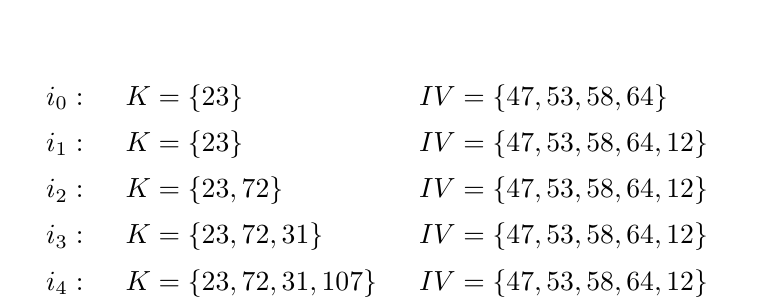
\begin{tikzpicture}[scale=1.0, every node/.style={scale=1.0}]
	\matrix (m)[matrix of nodes,column sep=3mm,row sep=0mm,align=left,nodes={anchor=base west},ampersand replacement=\&]
	{
		\node{$i_0:$}; \& \node{$K = \{23\}$}; \& $IV = \{47, 53, 58, 64\}$ \\
		\node{$i_1:$}; \& \node{$K = \{23\}$}; \& $IV = \{47, 53, 58, 64, 12\}$ \\
		\node{$i_2:$}; \& \node{$K = \{23, 72\}$}; \& $IV = \{47, 53, 58, 64, 12\}$ \\
		\node{$i_3:$}; \& \node{$K = \{23, 72, 31\}$}; \& $IV = \{47, 53, 58, 64, 12\}$ \\
		\node{$i_4:$}; \& \node{$K = \{23, 72, 31, 107\}$}; \& $IV = \{47, 53, 58, 64, 12\}$	\\
	};
	\end{tikzpicture}
\end{center}

The algorithm, in iteration $i_0$ starts with the optimal subset of size 5. In iteration $i_1$ all possible remaining bits are tried, and the best bit, i.e. the one giving the longest initial sequence of zeros, is selected and included in the subset, in this case IV bit 12. The algorithm then repeat the same step for all remaining iterations until a subset of the desired size is found, in this example $|S|=9$.

This greedy algorithm has the same drawbacks as for greedy algorithms in general---they may not find the global optimum, but rather get stuck in a local optima, thus resulting in a poor selection of $S$.

% XXX: rewritten
\section{Improved Algorithm} \label{sec:improvedalg}

Considering the possible issues of the greedy algorithm presented in the previous section, we propose a more general solution which can achieve better results. The main idea to solve this efficiency problem is to extend the na\"{i}ve greedy algorithm to examine more possible paths.

Rather than only considering the single best candidate in each iteration, our improved algorithm will store and explore a multitude of possible paths.
The rationale behind this approach is that the second best candidate in one iteration may be better in the following iteration of the algorithm, when more bits are to be added.

\begin{figure}[t]
	\begin{center}
		\tikzstyle{vecArrow} = [thick, decoration={markings,mark=at position
			1 with {\arrow[semithick]{open triangle 60}}},
		double distance=1.4pt, shorten >= 5.5pt,
		preaction = {decorate},
		postaction = {draw,line width=1.4pt, white,shorten >= 4.5pt}]
		\begin{tikzpicture}
		[node distance=.5cm,auto,>=latex',scale=0.9, every node/.style={scale=0.9},
		brcb/.style = {decoration={brace,pre=moveto,pre length=10pt,post=moveto,post length=10pt,raise=0.5mm, amplitude=3pt}, decorate},
		%		shorten <>/.style = {shorten >=#1pt, shorten <=#1pt},
		brcbl/.style = {decoration={brace,pre=moveto,pre length=10pt,post=moveto,post length=10pt,raise=0.5mm, amplitude=3pt}, decorate},
		%		shorten <>/.style = {shorten >=#1pt, shorten <=#1pt},
		brcbm/.style = {decoration={brace,pre=moveto,pre length=5pt,post=moveto,post length=5pt,raise=0.5mm,mirror,amplitude=3pt}, decorate},
		%		shorten <>/.style = {shorten >=#1pt, shorten <=#1pt}
		]
		\def\thecolsep{2pt}
		% Ugly hack to get a consistent image size.
		%\draw[use as bounding box] (-1.8,-4) rectangle (11.5,4);
		% i=0
		\node (A) {
			$\arraycolsep=\thecolsep \left[\begin{array}{ccc}
			2 &    ,   & 16 \\
			8 &    ,   & 43 \\
			32 &    ,   & 69 \\
			%				 9 &    ,   & 12 \\
			& \vdots & \\
			\end{array}\right]$
		};
		\draw [brcbm] (A.north west) -- (A.south west) node[midway,xshift=-2.1cm] {\small $\ldots k_{i-1} \alpha_{i-1}$};
		%\draw [brcb]  (A.north west) -- (A.north east) node[midway,yshift=0.2cm] {$n_{i-1}$};
		
		% i=1
		\node[above right=0.5cm and 1cm of A] (B1) {
			$\arraycolsep=\thecolsep \left[\begin{array}{ccccc}
			2 & , & 16 &   ,    & 86 \\
			2 & , & 16 &   ,    & 55 \\
			&   &    \vdots \\
			\end{array}\right]$
		};
		\draw [brcbm] (B1.north west) -- (B1.south west) node[midway,xshift=-0.7cm] {$k_i$};
		\draw [brcbl]  (B1.north) -- (B1.north east) node[midway,xshift=0pt,yshift=0.1cm] {$n_i$};
		
		\node[right=1cm of A] (B2) {
			$\arraycolsep=\thecolsep \left[\begin{array}{ccccc}
			8 & , & 43 &   ,    & 54 \\
			8 & , & 43 &   ,    & 27 \\
			&   &    \vdots \\
			\end{array}\right]$
		};
		\draw [brcbm] (B2.north west) -- (B2.south west) node[midway,xshift=-0.7cm] {$k_i$};
		\draw [brcbl]  (B2.north) -- (B2.north east) node[midway,xshift=0pt,yshift=0.1cm] {$n_i$};
		
		\node[below right=0.5cm and 1cm of A] (B3) {
			$\arraycolsep=\thecolsep \left[\begin{array}{ccccc}
			32 & , & 69 &   ,    & 5 \\
			32 & , & 69 &   ,    & 8 \\
			&   &    \vdots \\
			\end{array}\right]$
		};
		\draw [brcbm] (B3.north west) -- (B3.south west) node[midway,xshift=-0.7cm] {$k_i$};
		\draw [brcbl]  (B3.north) -- (B3.north east) node[midway,xshift=0pt,yshift=0.1cm] {$n_i$};
		
		% Arrows to Bx
		\coordinate (Afirst) at ([xshift=-0.2cm,yshift=-0.25cm]A.north east);
		\coordinate (Asecond) at ([yshift=-0.40cm]Afirst);
		\coordinate (Athird) at ([yshift=-0.40cm]Asecond);
		\draw[->,thick] (Afirst) -- (B1.west);
		\draw[->,thick] (Asecond) -- (B2.west);
		\draw[->,thick] (Athird) -- (B3.west);
		
		% sort, merge, and reduce step.
		\node[right=2.6cm of B2] (BM) {
			$\arraycolsep=\thecolsep \left[\begin{array}{ccccc}
			8 & , & 43 & , & 54 \\
			2 & , & 16 & , & 86 \\
			8 & , & 43 & , & 27 \\
			&   &   \vdots \\
			\end{array}\right]$
		};
		\draw [brcbm] (BM.north west) -- (BM.south west) node[midway,xshift=-2.8cm] {\small $\ldots k_{i-1} \alpha_{i-1} k_i \alpha_i$};
		
		\draw[vecArrow] ([yshift=1.2cm]B2.east) --  node {\scriptsize merge, sort, reduce} ([yshift=1.2cm]BM.west);
		\end{tikzpicture}
	\end{center}
	\caption{One step of our improved algorithm \cite{karlsson:2017}}
	\label{fig:overview}
\end{figure}

Increasing the number of explored candidates in each step of the algorithm will of course increase the computational complexity of the algorithm. We will, however, later derive the an expression for calculating the total computational effort required for certain parameters. In this way, we can easily estimate the computation time required.

The algorithm can briefly be described as follows:
The algorithm starts with either an optimal set of candidates, or an empty set. Each member of set is called a candidate, and every candidate is in itself a subset of key and IV-bits. For each candidate, the algorithm now tries to find the best bits to add, to maximize the initial sequence of zeros in the resulting MDM signature. This is done for each of the original candidates, which means that this generates several new sets of candidates. If this is repeated, the number of candidates clearly will grow to unmanageable numbers. Therefore, the algorithm limits the resulting set of new candidates with some factor.

A more formal and detailed description of the algorithm is described below. A description in pseudo-code can be found in \algref{slightlygreedy} and \algref{findbest}. The algorithm is parametrized by three different parameter vectors: $\bm{\alpha}$, $\bm{k}$, and $\bm{n}$. We also provide a graphical presentation of one iteration of the algorithm in \autoref{fig:overview}, which we will refer to in the more detailed, textual, description below:

\begin{enumerate}
	\item Consider a set of candidates from a previous iteration, or from an optimal starting set. If this is the first iteration, it is also possible to start with a completely empty subset of key and IV bits. In that case the algorithm starts with a single candidate, where the MDM signature is calculated with all key and IV bits set to zero. \label{itm:improvedalgfirst}
	\item For each candidate in the list, the algorithm adds the $k_i$ best $n_i$ new bits and store them in a new list. Note that there now exists one such new list for each candidate in the original list.
	\item Merge all lists, sorting by the number of zeros in the MDM signature. This gives a list of $k_0\alpha_0\ldots k_{i-1} \alpha_{i-1} k_i$ items, since there were $k_0\alpha_0\ldots k_{i-1} \alpha_{i-1}$ candidates in the beginning of this iteration, and each one has now resulted in $k_i$ new candidates.
	\item Finally, reduce the size of this merged list with the factor $\alpha_{i}$ ($0 < \alpha_i \le 1.0$), limiting the size of the combined list to $k_0\alpha_0\ldots k_{i-1} \alpha_{i-1} k_i \alpha_i$ items. If this step is omitted, or if $\alpha_i$ is set to $1.0$, the number of candidates will grow exponentially.
	\item Repeat from step~\ref{itm:improvedalgfirst} until a subset $S$ of the wanted size has been found.
\end{enumerate}

We earlier stated that this improved algorithm was a more general approach compared to the na\"{i}ve greedy algorithm described in \autoref{sec:greedybackground}. Using our new, improved algorithm and its input parameters $\bm{k}$, $\bm{n}$, and $\bm{\alpha}$, we can express the previous greedy algorithm's behavior as a specific set of input parameters, namely $\bm{\alpha} = [1.0, 1.0, \ldots])$, $\bm{k} = [1, 1, \ldots]$, and $\bm{n} = [n, n, \ldots]$. Thus our improved algorithm is a generalization of the previous algorithm, with many more degrees of freedom.

\alg{SlightlyGreedy \cite{karlsson:2017}}{alg:slightlygreedy}
{
	\textbf{Input:} key $K$, IV $V$, bit space $B$, maximum subset size $m$, vector $\bm{k}$, vector $\bm{n}$, vector $\bm{\alpha}$ \\
	\textbf{Output:} subset $S$ of size $m$.
}
{
	$S_0 = \{\emptyset\}$ \\
    /* The set $S_0$ contains a single empty subset */\\
	\cfor{} (each $i \in \{0, \ldots, m - 1\}$) \{ \\
	\indent\hspace{0.4cm}\cfor{} (each $c \in S_i$) \{ \\
	\indent\hspace{0.8cm}    $L_c$ = FindBest($K, V, B, c, k_i, n_i$); \\
	\indent\hspace{0.4cm}\} \\
	\indent\hspace{0.4cm}$S_{i+1}$ = concatenate(all $L_c$ from above); \\
	\indent\hspace{0.4cm}sort $S_{i+1}$ by the number of consecutive zeros in the MDM signature; \\
	\indent\hspace{0.4cm}reduce the number of elements in $S_{i+1}$ by a factor $\alpha_i$; \\
	\} \\
	\creturn{} $S_m$;
}

\alg{FindBest \cite{karlsson:2017} }{alg:findbest}
{
	\textbf{Input:} key $K$, IV $V$, bit space $B$, current subset $c$, number of best subsets to retain $k$, bits to add $n$ \\
	\textbf{Output:} $k$ subsets each of size $|c| + n$.
}
{
	/* let $\binom{S}{k}$ denote the set of all $k$-combinations of a set $S$. */ \\
	\\
	$S = \emptyset$; \\
	\cfor{} (each $n$-tuple $\{b_1, \ldots, b_n\} \in \binom{B\setminus c}{n}$) \{ \\
	\indent\hspace{0.4cm}$z = $ number of initial zeros using subset $c \cup \{b_1, \ldots, b_n\}$; \\
	\indent\hspace{0.4cm}\cif{} ($z$ is among the $k$ highest values) \{ \\
	\indent\hspace{0.8cm}    add $c \cup \{b_1, \ldots, b_n\}$ to $S$; \\
	\indent\hspace{0.8cm}    reduce $S$ to $k$ elements by removing element with lowest $z$; \\
	\indent\hspace{0.4cm}\} \\
	\} \\
	\creturn{} $S$;
}

\subsection{Computational Cost}
The improved algorithm may have a greater computation cost compared to the previous greedy algorithm, because it considers more candidates. The computational cost will depend on the input parameter vectors, since they affect the amount of candidates explored.

The total computational cost $C$ is expressed as the number of initializations required. The cost is expressed according to the following function, from \cite{karlsson:2017}, where $c$ is the number of iterations required ($c=|\bm{k}|=|\bm{n}|=|\bm{\alpha}|$), and $b$ is the bit space size $b=|B|$.

\begin{align}
C(b, c, \bm{k}, \bm{n}, \bm{\alpha}) = 
\sum_{i=0}^{c-1} \left[ 2^{\sum_{j=0}^{i} n_j} \binom{b - \sum_{j=0}^{i-1} n_j}{n_i} \prod_{j=0}^{i-1} k_j \alpha_j \right]
\label{eq:complexity}
\end{align}

The expression can be derived using combinatorics. In the expression, the power of two is related to the size of the different subsets $S$---a large subset requires more initializations of the cipher. The binomial coefficient is the number of possible subsets we can form given the current iteration's $n_i$. Finally, the final product is needed because the algorithm reduces the number of candidates in each iteration using the factors in $\bm{\alpha}$.
Clearly, in practice, the actual running time is also dependent on other factors, such as the cipher we are running the algorithm on.

As a special case of the expression in \autoref{eq:complexity}, an expression for the previous greedy algorithm can be derived. Recall that this algorithm had a constant $n$, and since it only considered the best candidate in each iteration, both $\bm{k}$ and $\bm{\alpha}$ are all ones. Under these constraints, the expression can more concisely be given as \cite{karlsson:2017}:

\begin{align}
C(b, c, n) = \sum_{i=0}^{c-1} \left[ 2^{n(i+1)} \binom{b - n \cdot i}{n} \right]
\label{eq:complexitygreedy}
\end{align}


%or if one-indexed:
%\begin{align}
%C(b, c, \bm{k}, \bm{n}, \bm{\alpha}) = \sum_{i=1}^{c} \left[ 2^{\sum_{j=1}^{i} n_j} \binom{b - \sum_{j=1}^{i-1} n_j}{n_i} \prod_{j=1}^{i-1} k_j \alpha_j \right]
%\label{eq:complexityoneindex}
%\end{align}

\section{Results} \label{sec:results}
To get any results from our proposed algorithm, the choice of parameters must first be discussed. The algorithm is parametrized by the parameter vectors $\bm{k}$, $\bm{n}$, and $\bm{\alpha}$. In this section we will explore and investigate how the choice of parameters affect the final result of our algorithm. These new results will be compared to the previous greedy algorithm as a baseline.

The greedy algorithm only had one degree of freedom, $n$, while the improved algorithm has many more. We have performed a significant amount of simulations, on several different ciphers, to be able to present results on how the choice of parameters affect the results of the algorithm.

The tests have been performed on the stream ciphers Grain-128a \cite{agren:2011}, Kreyvium \cite{canteaut:2016}, and to some extent Grain-128 \cite{hell:2006b}. For reference, the exact parameters used for each result presented below are available in the Appendix of this paper.

\subsection{Tuning the Greediness} \label{sec:tuninggreedy}

To get a feeling for how the different parameters affect the result, we start by varying the two parameter vectors $\bm{k}$ and $\bm{\alpha}$, while keeping $\bm{n}$ consistent, and equal to an all-one vector.
While $\bm{k}$ and $\bm{\alpha}$ gives almost unlimited possibilities, we have opted for the following simulation setup.

For every test case, a given iteration $i$ will have the same amount of candidates, which makes the computational complexity identical between the different test cases. The input vectors $\bm{k}$ and $\bm{\alpha}$ will of course be different for the different test cases, which in turn mean that even if the amount of candidates is the same, the actual candidates will vary between the tests. By designing the test this way, we wish to investigate how this difference in candidate selection affect the final result of the algorithm.

Recall that $k_i$ govern how many new candidates we generate from a previous iteration's subsets. A high $k_i$ and low $\alpha_i$ means that we may end up with several candidates that have the same ``stem'', i.e. they have the same origin list. If we lower $k_i$ and instead increase $\alpha_i$ we will get a greater mix of different stems, while still maintaining the same amount of candidates for the iteration---in a sense the greediness of the algorithm is reduced. Thus, we want to test some different tradeoffs between the two parameters. In the results below, we name the different test cases as a percentage value of the total amount of candidates for each round. As an example, if the total number of candidates in a given round is 1000, we could select a $k_i$ of 200, and a corresponding $\alpha_i$ of $0.005$, which gives us 1000 candidates for the next round as well. We call this particular case \emph{20 \%-k} since $k_i$ is 20~\% of the candidates for the round.

As mentioned earlier, the simulations have been performed on different ciphers, in this case Grain-128a and Kreyvium.
We have tried several combinations of $\bm{k}$ and $\bm{\alpha}$ as can be seen in the plot in \autoref{fig:kalpha}, which includes one plot for each cipher. Note that Grain-128a has 256 initialization rounds, while Kreyvium has 1152 initialization rounds.
The greedy algorithm is also included as a reference. Note that the greedy algorithm will, due to its simplistic nature, have a lower computational complexity since it only keeps one candidate in each iteration. To be able to compare the results based on computational complexity, we have plotted the graph based on logarithmic complexity rather than subset size. The complexity is calculated using Equation~\ref{eq:complexity}, and the natural logarithm is then applied on this value, so that a reasonably scaled plot is produced. This graph can be seen in \autoref{fig:kalphacomplexity}, for the same ciphers as above. The maximum values for each case is also available in \autoref{tbl:kalpha}.

From the results we note that a too low $k$ seems to lower the efficiency of the algorithm. The reason for this is probably that a too low $k$ forces the algorithm to choose candidates from lists with lower value. These candidates are then poor choices for the upcoming iterations. We also note that our improved algorithm consistently gives better results than the previous greedy algorithm.

%\renewcommand{\arraystretch}{1.2} 
\begin{table}[htb]
	\centering
    \caption{Maximum length of initial sequence of zeros in MDM signature when varying $\bm{k}$ and $\bm{\alpha}$, expressed as actual count, and percentage of total initialization rounds}
    \begin{tabular}{lrrrr}
    	\toprule
        & \multicolumn{2}{c}{Grain-128a} & \multicolumn{2}{c}{Kreyvium} \\
        \cmidrule(r){2-3} \cmidrule(l){4-5}
                  & Count & Percentage & Count & Percentage \\
        \midrule
        Greedy & 187 & 73.0 & 862 & 74.8 \\
        20 \%-k & 203 & 79.3 & 896 & 77.8 \\
        0.5 \%-k & 198 & 77.3 & 876 & 76.0 \\
        0.2 \%-k & 192 & 75.0 & 877 & 76.1 \\ 
        min-k \%-k & 190 & 74.2 & 866 & 75.2 \\
        \bottomrule
    \end{tabular}
    \label{tbl:kalpha}
\end{table}

\begin{figure}[htbp]
	\centering
	\begin{subfigure}[b]{0.5\textwidth}
		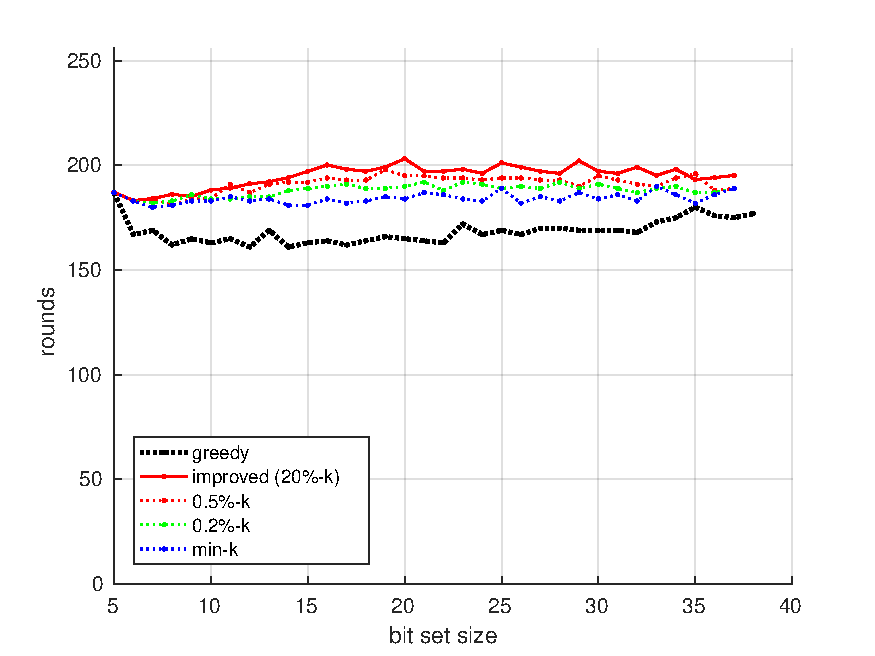
\includegraphics[width=1.07\columnwidth]{kalpha_pres1}
		\captionsetup{singlelinecheck=true}
		\caption{Grain-128a}
		\label{fig:kalphagrain128a}
	\end{subfigure}%
	\begin{subfigure}[b]{0.5\textwidth}
		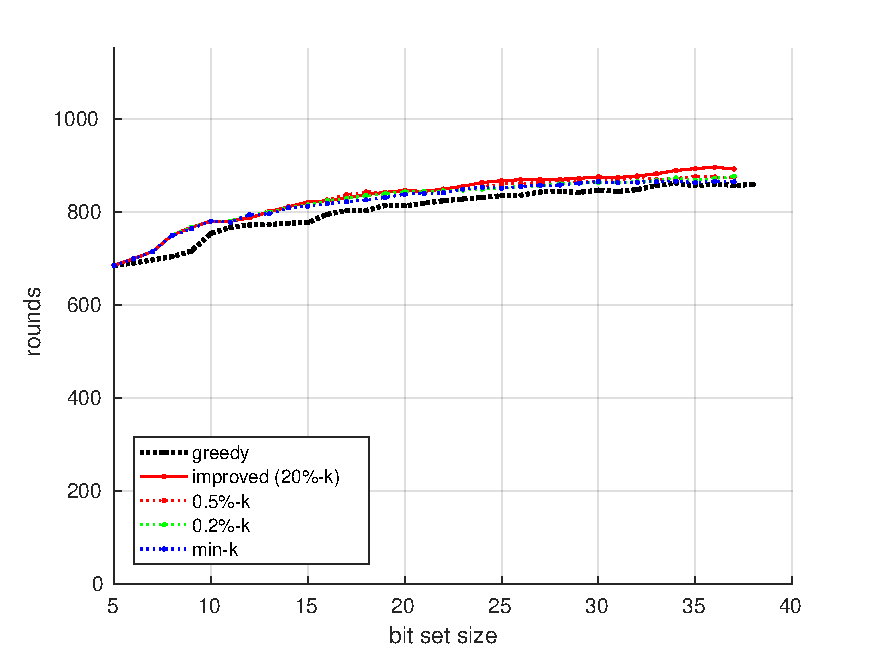
\includegraphics[width=1.07\columnwidth]{kalpha_pres1_kreyvium}
		\captionsetup{singlelinecheck=true}
		\caption{Kreyvium}
		\label{fig:kalphakreyvium}
	\end{subfigure}	
	\caption{Varying $k$ and $\alpha$, with $n_i=1$. Thick dotted black line is the greedy baseline.}
	\label{fig:kalpha}
\end{figure}

\begin{figure}[htbp]
	\centering
	\begin{subfigure}[b]{0.5\textwidth}
		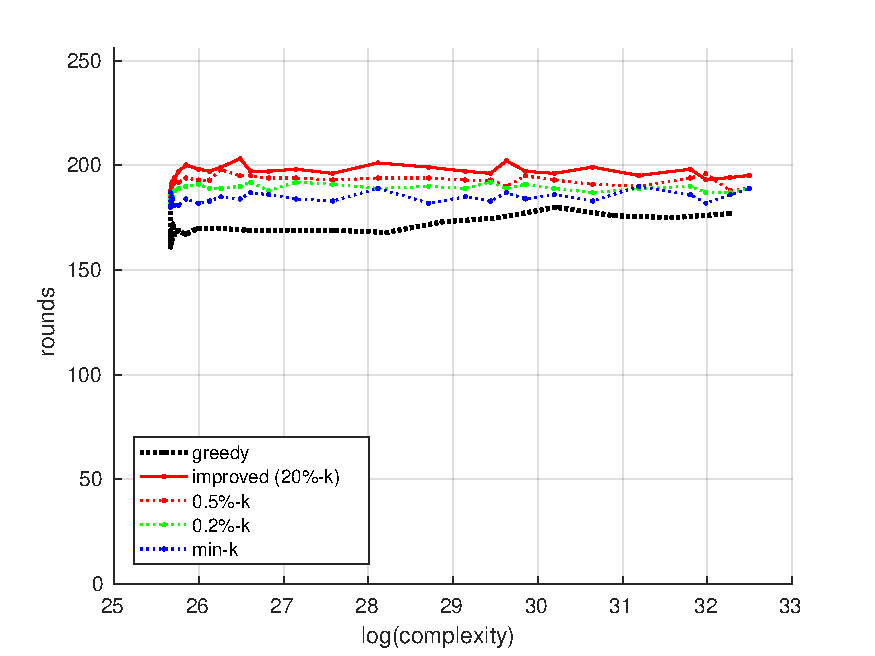
\includegraphics[width=1.07\columnwidth]{kalpha_pres1_complexity}
		\captionsetup{singlelinecheck=true}
		\caption{Grain-128a}
		\label{fig:kalphacomplexitygrain128a}
	\end{subfigure}%
	\begin{subfigure}[b]{0.5\textwidth}
		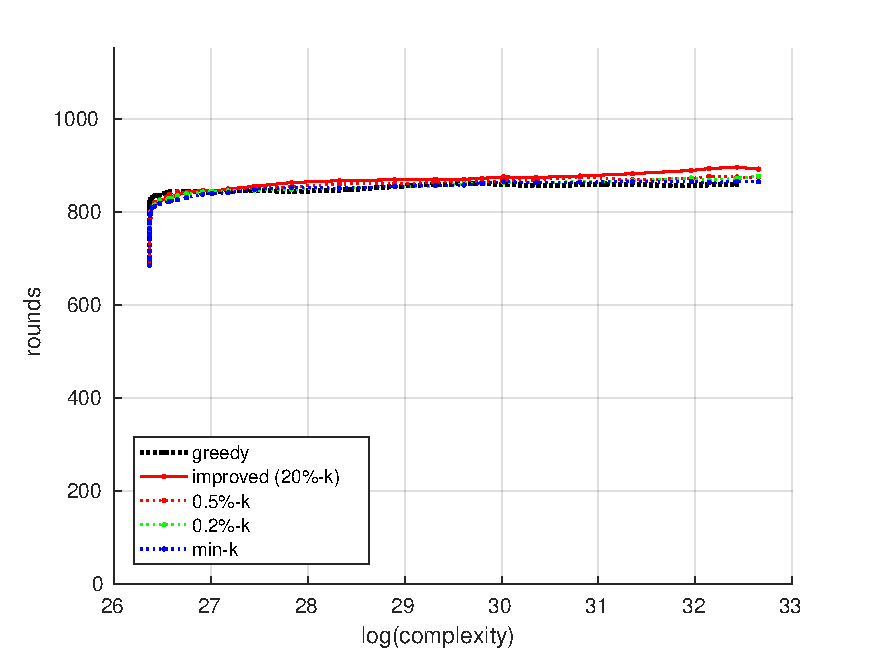
\includegraphics[width=1.07\columnwidth]{kalpha_pres1_kreyvium_complexity}
		\captionsetup{singlelinecheck=true}
		\caption{Kreyvium}
		\label{fig:kalphacomplexitykreyvium}
	\end{subfigure}
	
	\caption{Varying $k$ and $\alpha$, with $n_i=1$. Thick dotted black line is the greedy baseline. The $x$-axis scaled according to logarithmic computational complexity.}
	\label{fig:kalphacomplexity}
\end{figure}

%\subsection{Varying $\bm{n}$}
\subsection{Varying the Number of Bits Added in Each Iteration}

In the previous section, a fixed $\bm{n}$ was used throughout all tests. In this section, we will instead focus on the input parameter vector $\bm{n}$ and see how different vectors affect the result of the algorithm. Recall that this vector decides how many bits that is added to the subset in each iteration.

Intuitively, we expect a higher value of a single $n_i$ to yield better results, since this also reduces the risk to get stuck in a local optima. However, having a large, constant $n_i$ in all iterations, as explored in \cite{stankovski:2010}, means that later iterations will be require very heavy computations. We therefore explore three different variants, where the vector $\bm{n}$ contains decreasing values of $n_i$. These results are then compared to the previous greedy approach where a constant $n$ of different values where used throughout the whole algorithm.

For these tests, the computational complexity will vary between the different tests. This is different from the previous section where the tests were designed to have the same computational complexity. Therefore the results are once again presented in two ways, first as plots where the $x$-axis is the subset size, as seen in \autoref{fig:n}.
The other plots present the results plotted by their computational complexity. As in the last section, the complexity is calculated using \autoref{eq:complexity}, and the plot uses a logarithmic scale on the $x$-axis. This can be seen in \autoref{fig:ncomplexity}. The results for each test case are also available in tabular form in \autoref{tbl:n}.

From the results we note that regardless of our choice of $\bm{n}$, our algorithm outperforms the greedy variants. For Grain-128a, we also see that a higher $n_i$ in the initial iterations seem to lead to better results which remain as the algorithm proceeds towards larger subsets. The results for Kreyvium are not as clear, and it seems like the size of the resulting subset is the most important property.

% allow three consecutive floats.
%\setcounter{topnumber}{3}

\begin{table}[htb]
	\centering
    \caption{Maximum length of initial sequence of zeros in MDM signature when varying $\bm{n}$, expressed as actual count, and percentage of total initialization rounds}
    \begin{tabular}{lrrrr}
    	\toprule
        & \multicolumn{2}{c}{Grain-128a} & \multicolumn{2}{c}{Kreyvium} \\
        \cmidrule(r){2-3} \cmidrule(l){4-5}
                  & Count & Percentage & Count & Percentage \\
        \midrule
        Greedy 1-bit & 187 & 73.1 & 862 & 74.8 \\
        Greedy 2-bit & 187 & 73.1 & 864 & 75.0 \\
        Greedy 3-bit & 187 & 73.1 & 851 & 73.9 \\
        2-2-2-2-2-2-2-2-1-\ldots & 203 & 79.3 & 868 & 75.4 \\
        2-2-2-2-1-\ldots & 199 & 77.7 & 872 & 75.7 \\
        1-\ldots & 195 & 76.2 & 869 & 75.4 \\ 
        \bottomrule
    \end{tabular}
    \label{tbl:n}
\end{table}


\begin{figure}[htbp]
	\centering
	\begin{subfigure}[b]{0.5\textwidth}
		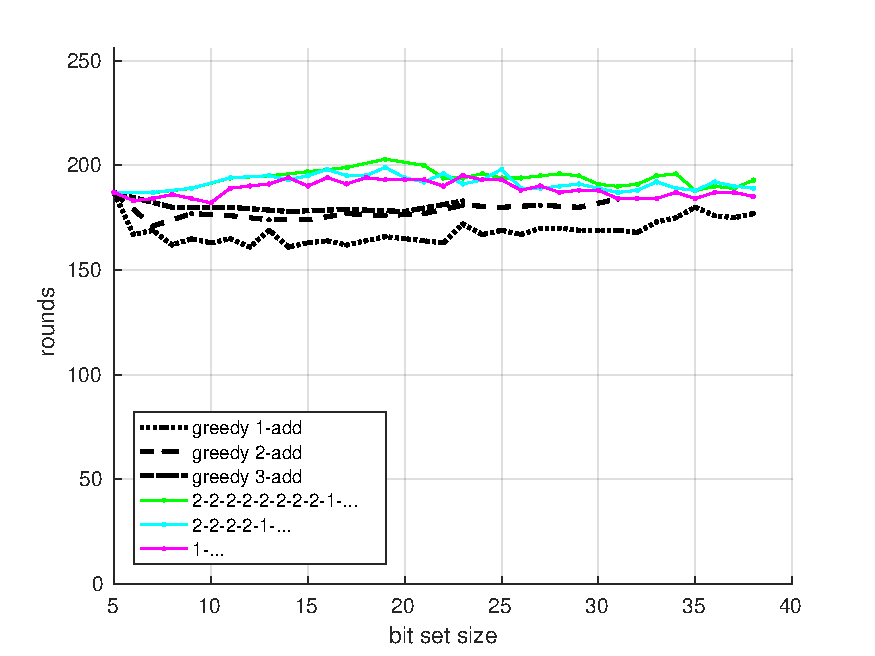
\includegraphics[width=1.07\columnwidth]{nstat_pres}
		\captionsetup{singlelinecheck=true}
		\caption{Grain-128a}
		\label{fig:ngrain128a}
	\end{subfigure}%
	\begin{subfigure}[b]{0.5\textwidth}
		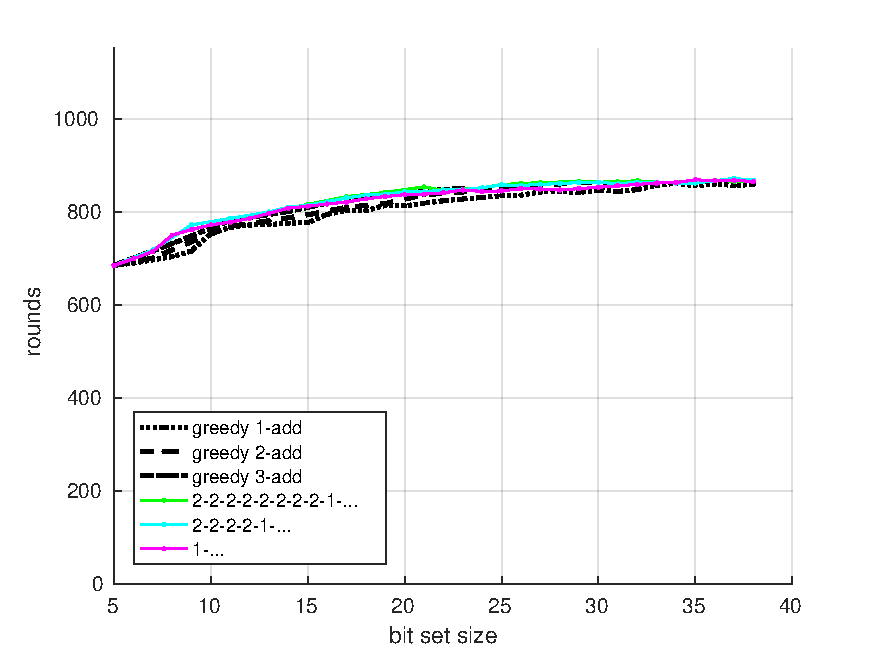
\includegraphics[width=1.07\columnwidth]{nstat_pres_kreyvium}
		\captionsetup{singlelinecheck=true}
		\caption{Kreyvium}
		\label{fig:nkreyvium}
	\end{subfigure}
	
	\caption{Varying $n$. Thick black lines are the greedy baselines for $n$ equal to 1, 2, and 3.}
	\label{fig:n}
\end{figure}

\begin{figure}[htbp]
	\centering
	\begin{subfigure}[b]{0.5\textwidth}
		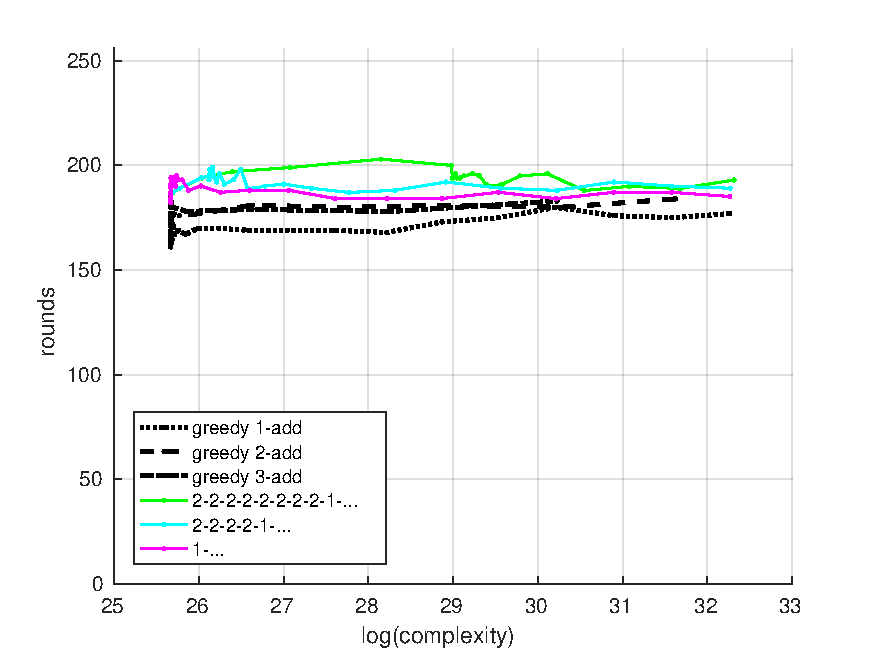
\includegraphics[width=\columnwidth]{nstat_pres_complexity}
		\captionsetup{singlelinecheck=true}
		\caption{Grain-128a}
		\label{fig:ncomplexitygrain128a}
	\end{subfigure}%
	\begin{subfigure}[b]{0.5\textwidth}
		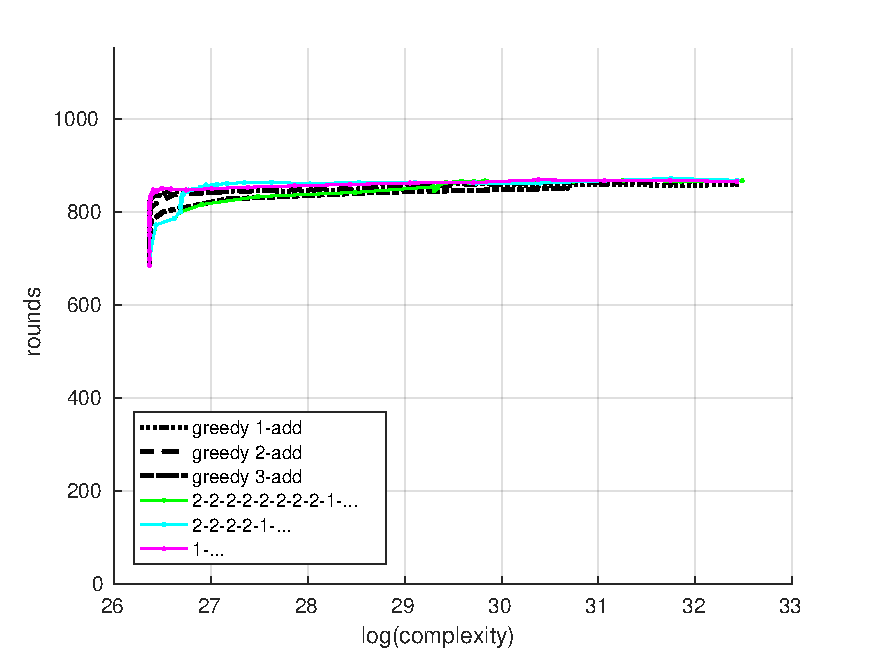
\includegraphics[width=\columnwidth]{nstat_pres_kreyvium_complexity}
		\captionsetup{singlelinecheck=true}
		\caption{Kreyvium}
		\label{fig:ncomplexitykreyvium}
	\end{subfigure}
	
	\caption{Varying $n$. Thick black lines are the greedy baselines for $n$ equal to 1, 2, and 3. The $x$-axis scaled according to logarithmic computational complexity.}
	\label{fig:ncomplexity}
\end{figure}

\subsection{Results for Different Starting Points}

In the previous tests, optimal subsets of size 5 has been used as a starting point for the simulations. In this section, we compare the use of such an optimal start to starting from an empty subset. A simple approach has been chosen, namely to reuse two test cases from \autoref{sec:tuninggreedy}, namely the test case named 20~\%-k for both Grain-128a and Kreyvium. These test cases start with optimal subsets of size 5.

The two new additional test cases start with an empty subset, and then sequentially add one bit during the first five iterations. The remaining  iterations' parameters are kept the same between all test cases, so that the difference in the initial start is isolated. In this way we can investigate whether this optimal starting set is important or not.

The result of this experiment can be found in \autoref{fig:startingset}, again with one subfigure for Grain-128a and one for Kreyvium. The results are summarized in \autoref{tbl:startingset}. In summary, the differences are very small, and for Kreyvium non-existent, which means that the choice of initial starting point may not be the most important decision to make when selecting parameters for the algorithm.

\begin{table}[htb]
	\centering
    \caption{Maximum length of initial sequence of zeros in MDM signature with different starting subsets, expressed as actual count, and percentage of total initialization rounds}
    \begin{tabular}{lrrrr}
    	\toprule
        & \multicolumn{2}{c}{Grain-128a} & \multicolumn{2}{c}{Kreyvium} \\
        \cmidrule(r){2-3} \cmidrule(l){4-5}
                  & Count & Percentage & Count & Percentage \\
        \midrule
        5-bit optimal start & 203 & 79.3 & 896 & 77.8 \\
        Empty subset start & 201 & 78.5 & 896 & 77.8 \\
        \bottomrule
    \end{tabular}
    \label{tbl:startingset}
\end{table}


\begin{figure}[htbp]
	\centering
	\begin{subfigure}[b]{0.5\textwidth}
		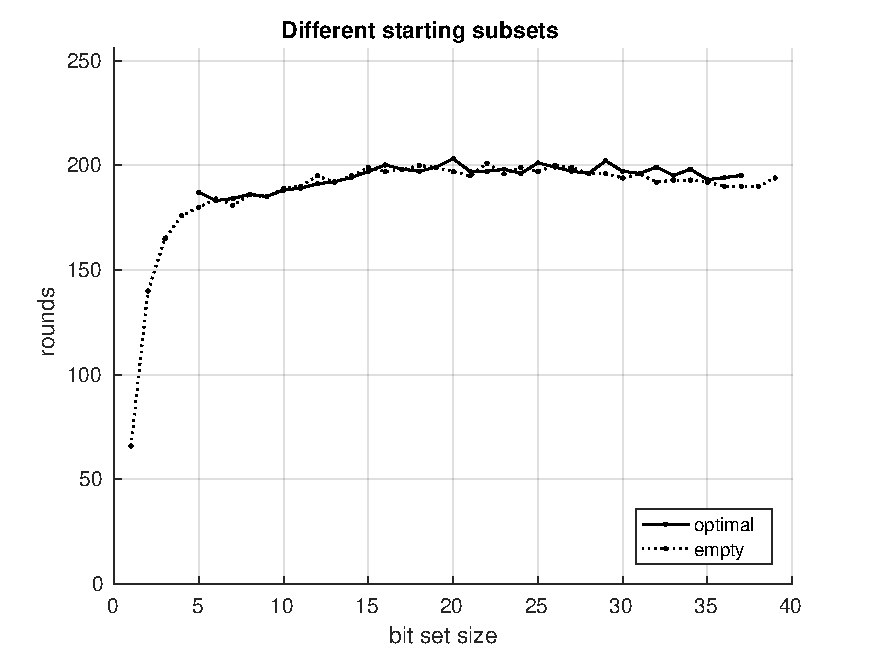
\includegraphics[width=1.07\columnwidth]{startingset_pres_grain128a}
		\captionsetup{singlelinecheck=true}
		\caption{Grain-128a}
		\label{fig:startingsetgrain128a}
	\end{subfigure}%
	\begin{subfigure}[b]{0.5\textwidth}
		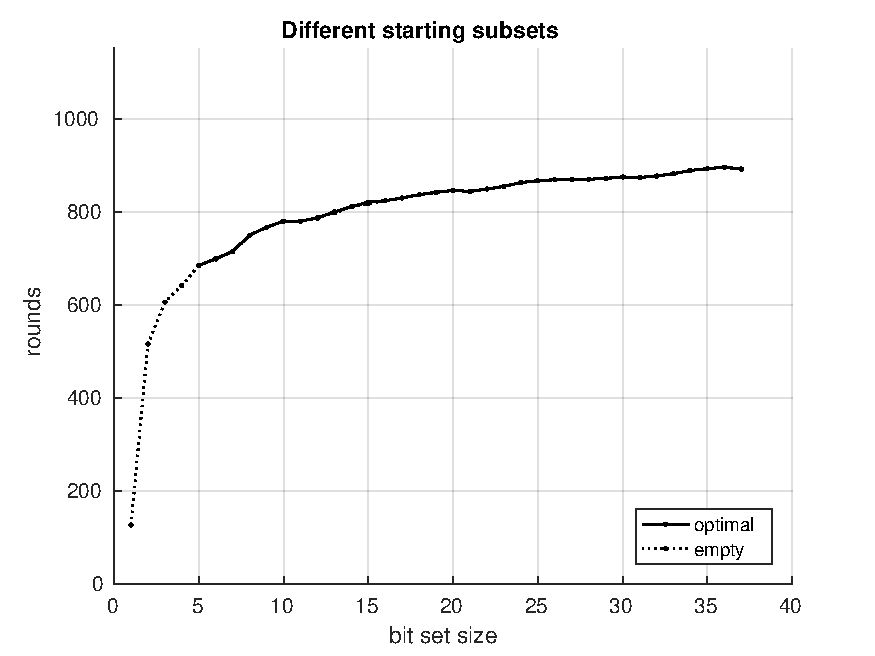
\includegraphics[width=1.07\columnwidth]{startingset_pres_kreyvium}
		\captionsetup{singlelinecheck=true}
		\caption{Kreyvium}
		\label{fig:startingsetkreyvium}
	\end{subfigure}
	
	\caption{Different starting sets and how they affect the results}
	\label{fig:startingset}
\end{figure}

\subsection{Results on Grain-128}
% results for good old grain-128, where we actually found a 256/256 bitset fairly fast.

Apart from new results on Grain-128a and Kreyvium, tests were also performed on Grain-128, a predecessor of Grain-128a which has been analyzed in other works. In \cite{stankovski:2010}, a full-round (256 out of 256 initialization rounds) result was presented using a subset of size 40, using only IV-bits, with an optimal starting subset of size 6. This was found using a constant $n=2$. This corresponds to a parameter set of $\bm{\alpha} = [1.0, 1.0, 1.0, \ldots])$, $\bm{k} = [1, 1, 1, \ldots]$, and $\bm{n} = [6, 2, 2, \ldots]$ in our improved algorithm.

It would clearly be possible to find the exact same subset using our improved algorithm, but we are also interested in seeing whether or not we can find other subsets resulting in full-round results using our improved algorihtm.
A new set of parameters for our improved algorithm is constructed as follows:
The possibility to keep multiple candidates in each step is utilized, especially in the beginning where there are still small subsets. Using the improved algorithm, a smaller subset of size 25 is found, which still gives us a full-round result of 256 out of 256 initialization rounds.

Using the complexity expression in Equation~\ref{eq:complexity}, the computational complexity between the two results can be compared. We find that our improved algorithm has a complexity which is a factor about $2^{12}$ lower than the earlier result, while still finding an equal amount of zeros in the MDM signature.

\section{Related Work} \label{sec:slightlygreedy:relatedwork}

Related work can be divided into two main categories: work related to the maximum degree monomial test, and work related to general cryptanalysis of the discussed ciphers. 

In \cite{saarinen:2006}, Saarinen described the $d$-Monomial test, and how it can be applied in chosen-IV attacks against stream ciphers. In contrast to our work, and the work done by Stankovski \cite{stankovski:2010}, Saarinen considers monomials of various degrees, namely monomials up to degree $d$, therefore the name $d$-Monomial test. In addition to this difference, the choice of input subset bits is different. Saarinen only considers consecutive bits either in the beginning or in the end of the IV. This is in contrast to our work, where the subset is chosen freely as any subset of IV and/or key bits.

Related to the work of Saarinen, the Maximum Degree Monomial (MDM) was introduced by Englund et. al. in \cite{englund:2007}. Rather than looking at several different degrees of monomials, the MDM test only focuses on the maximum degree monomial. The motivation behind this choice is that the maximum degree monomial is likely to occur only if all IV bits have been properly mixed. In addition to this, the existence of the maximum degree monomial is easy to find. The coefficient of the monomial can be found by simply XORing all entries in the truth table.

In the previously mentioned work, a subset of the IV space was used in the tests. In \cite{stankovski:2010}, a greedy heuristic to find these subsets was discussed. The greedy algorithm started with an optimal, precalculated, subset of a small size, and then added $n$ bits in each step in a greedy fashion. In addition, both IV and key bits were suggested for getting distinguisher and nonrandomness results, respectively. Several different ciphers were analyzed, among them Grain-128 and Trivium.

Other work related to distinguishers for Trivium is \cite{liu:2015}, where the authors concentrate on small cubes, and instead look at unions of these cubes. Another difference is that they look at sub-maximal degree monomial tests.

 % from: "Observing biases in the state: case studies with Trivium and Trivia-SC", Santanu Sarkar, Subhamoy Maitra, Anubhab Baksi, 
Also partly based on Stankovski's work is the work in \cite{sarkar:2016}, where the authors propose two new, alternative heuristics. Here, the heuristic is modified so that it does not maximize the initial sequence of zeros in the MDM signature. Rather, in the first heuristic, called ``maximum last zero'', the authors not only maximize the initial sequence of zeros, but also ensure that the position of the current iteration in the MDM signature is a zero as well. In their second heuristic, called ``maximum frequency of zero'', they instead look at the total amount of zeros in the MDM signature. Their heuristics are applied to the ciphers Trivium \cite{canniere:2006} and Trivia-SC \cite{chakraborti:2015}. Similar to our paper, they also mention the use of a non-constant $n$, i.e. a $\bm{n}$-vector, although the authors do not discuss the reasons for this extension.
% they also discuss tie cases, something we e.g. get "for free" in our algorithm as long as k > 1.

In \cite{vielhaber:2007} an attack called AIDA on a modified version of Trivium was presented. In this case Trivium was modified so that it only had half of the original count of initialization rounds. Related to this attack are the 
cube attacks \cite{dinur:2009}, and especially the dynamic cube attack \cite{dinur:2011} which was used to attack Grain-128.

% random attacks in general against grain-128a
Attacks on the newer Grain-128a can be found in the literature as well. In \cite{banik:2013} the authors present a related-key key attack requiring $>2^{32}$ related keys and $>2^{64}$ chosen IVs, while in \cite{sarkar:2014} the authors present a differential fault attack against all the three ciphers in the Grain-family.

% kreyvium analys: (new for extended paper)
There is very limited work regarding the analysis of Kreyvium, possibly because the original Kreyvium paper is relatively recent, however in \cite{watanabe:2017} the authors discuss conditional differential cryptanalysis of Kreyvium.

\section{Conclusions} \label{sec:slightlygreedy:conclusions}

This paper has described the design and motivation of the maximum degree monomial test when designing nonrandomness detectors. The MDM test requires a subset of key and IV bits, and in this paper we have designed and proposed a new algorithm to find such subsets. Our algorithm is based on a greedy approach, but rather than using a na\"{i}ve greedy algorithm, we propose an algorithm which is less likely to get stuck in local optima, and therefore yields better final results. The algorithm is highly flexible, and parameters can be chosen and adapted to get a both reasonable and predictable computational complexity. To validate our algorithm, we have performed a significant amount of simulations to find good input parameters to our algorithm. Simulations has been performed mainly on the ciphers Grain-128a and Kreyvium, and the results show that our new algorithm outperforms previously proposed na\"{i}ve greedy algorithms.

% DONE: rewritten
\section*{Acknowledgments}
This paper is an extended and revised version of the paper ``Improved Greedy Nonrandomness Detectors for Stream Ciphers'' previously presented at ICISSP 2017 \cite{karlsson:2017}.

The computations were performed on resources provided by the Swedish National Infrastructure for Computing (SNIC) at Lunarc.

%\vfill
%\bibliographystyle{splncs03}
%{
%\bibliography{slightlygreedy}}

{\raggedright
	\printbibliography[segment=\therefsegment,heading=subbibliography]
}

% Placed here to allow for top placement of the above table.
\section*{Appendix}%
\addcontentsline{toc}{section}{Appendix}%
\markright{Appendix}

This appendix contains the exact vectors used for the different results discussed in \autoref{sec:results}. The vectors used for the results for varying $\bm{k}$ and $\bm{\alpha}$ are given in \autoref{tbl:appkalpha}. In the same fashion, the vectors used for the results for varying $\bm{n}$ are presented in \autoref{tbl:appn}. Finally, the vectors for the results on Grain-128 are given in \autoref{tbl:appgrain128}.

\begin{table*}[htb]
	\centering
    \caption{Varying $\bm{k}$ and $\bm{\alpha}$ \cite{karlsson:2017}}
    \footnotesize
    \resizebox{\columnwidth}{!}{%
    \begin{tabular}{rp{11cm}}
    	\toprule
         & Greedy \\
        \midrule
        $\bm{k} $ & \{ 1, 1, 1, 1, 1, 1, 1, 1, 1, 1, 1, 1, 1, 1, 1, 1, 1, 1, 1, 1, 1, 1, 1, 1, 1, 1, 1, 1, 1, 1, 1, 1, 1, 1, 1 \} \\
        $\bm{n} $ & \{ 5, 1, 1, 1, 1, 1, 1, 1, 1, 1, 1, 1, 1, 1, 1, 1, 1, 1, 1, 1, 1, 1, 1, 1, 1, 1, 1, 1, 1, 1, 1, 1, 1, 1, 1 \} \\
        $\bm{\alpha}$ & \{ 1, 1, 1, 1, 1, 1, 1, 1, 1, 1, 1, 1, 1, 1, 1, 1, 1, 1, 1, 1, 1, 1, 1, 1, 1, 1, 1, 1, 1, 1, 1, 1, 1, 1, 1 \} \\
        \midrule

        & Improved (20 \%-k) \\
        \midrule
        $\bm{k} $ & \{ 1000, 200, 200, 200, 200, 200, 200, 200, 200, 200, 200, 200, 100, 60, 60, 20, 20, 20, 20, 20, 20, 12, 6, 3, 2, 2, 2, 2, 2, 1, 1, 1, 1 \} \\
        $\bm{n} $ & \{ 5, 1, 1, 1, 1, 1, 1, 1, 1, 1, 1, 1, 1, 1, 1, 1, 1, 1, 1, 1, 1, 1, 1, 1, 1, 1, 1, 1, 1, 1, 1, 1, 1 \} \\
        $\bm{\alpha}$ & \{ 1.0, 0.005, 0.005, 0.005, 0.005, 0.005, 0.005, 0.005, 0.005, 0.005, 0.005, 0.005, 0.005, 0.01, $\frac{1}{60}$, $\frac{1}{60}$, 0.05, 0.05, 0.05, 0.05, 0.05, 0.05, $\frac{1}{12}$, $\frac{2}{15}$, 0.375, 0.5, 0.5, 0.5, 0.5, $\frac{2}{9}$, 1.0, 0.5, 1.0 \} \\
        \midrule

        & 0.5 \%-k \\
        \midrule
        $\bm{k} $ & \{ 1000, 5, 5, 5, 5, 5, 5, 5, 5, 5, 5, 5, 3, 2, 2, 1, 1, 1, 1, 1, 1, 1, 1, 1, 1, 1, 1, 1, 1, 1, 1, 1, 1 \} \\
        $\bm{n} $ & \{    5, 1, 1, 1, 1, 1, 1, 1, 1, 1, 1, 1, 1, 1, 1, 1, 1, 1, 1, 1, 1, 1, 1, 1, 1, 1, 1, 1, 1, 1, 1, 1, 1 \}  \\
        $\bm{\alpha}$ & \{ 1.0, 0.2, 0.2, 0.2, 0.2, 0.2, 0.2, 0.2, 0.2, 0.2, 0.2, 0.2, $\frac{1}{6}$, 0.3, 0.5, $\frac{1}{3}$, 1.0, 1.0, 1.0, 1.0, 1.0, 0.6, 0.5, 0.4, 0.75, 1.0, 1.0, 1.0, 1.0, $\frac{2}{9}$, 1.0, 0.5, 1.0 \} \\
        \midrule

        & 0.2 \%-k \\
        \midrule
        $\bm{k} $ & \{ 1000, 2, 2, 2, 2, 2, 2, 2, 2, 2, 2, 2, 1, 1, 1, 1, 1, 1, 1, 1, 1, 1, 1, 1, 1, 1, 1, 1, 1, 1, 1, 1, 1 \} \\
        $\bm{n} $ & \{ 5, 1, 1, 1, 1, 1, 1, 1, 1, 1, 1, 1, 1, 1, 1, 1, 1, 1, 1, 1, 1, 1, 1, 1, 1, 1, 1, 1, 1, 1, 1, 1, 1 \} \\
        $\bm{\alpha}$ & \{ 1.0, 0.5, 0.5, 0.5, 0.5, 0.5, 0.5, 0.5, 0.5, 0.5, 0.5, 0.5, 0.5, 0.6, 1.0, $\frac{1}{3}$, 1.0, 1.0, 1.0, 1.0, 1.0, 0.6, 0.5, 0.4, 0.75, 1.0, 1.0, 1.0, 1.0, $\frac{2}{9}$, 1.0, 0.5, 1.0 \}  \\
        \midrule

        & min-k \\
        \midrule
        $\bm{k} $ & \{ 1000, 1, 1, 1, 1, 1, 1, 1, 1, 1, 1, 1, 1, 1, 1, 1, 1, 1, 1, 1, 1, 1, 1, 1, 1, 1, 1, 1, 1, 1, 1, 1, 1 \} \\
        $\bm{n} $ & \{ 5, 1, 1, 1, 1, 1, 1, 1, 1, 1, 1, 1, 1, 1, 1, 1, 1, 1, 1, 1, 1, 1, 1, 1, 1, 1, 1, 1, 1, 1, 1, 1, 1 \} \\
        $\bm{\alpha}$ & \{ 1.0, 1.0, 1.0, 1.0, 1.0, 1.0, 1.0, 1.0, 1.0, 1.0, 1.0, 1.0, 0.5, 0.6, 1.0, $\frac{1}{3}$, 1.0, 1.0, 1.0, 1.0, 1.0, 0.6, 0.5, 0.4, 0.75, 1.0, 1.0, 1.0, 1.0, $\frac{2}{9}$, 1.0, 0.5, 1.0 \}  \\
        \bottomrule
    \end{tabular}%
	}
    \label{tbl:appkalpha}
\end{table*}

\begin{table*}[tbp]
	\centering
    \caption{Varying $\bm{n}$ \cite{karlsson:2017}}
    \footnotesize
    \resizebox{\columnwidth}{!}{%
    \begin{tabular}{rp{11.1cm}}
    	\toprule
         & Greedy 1-add\\
        \midrule
        $\bm{k} $ &     \{ 1, 1, 1, 1, 1, 1, 1, 1, 1, 1, 1, 1, 1, 1, 1, 1, 1, 1, 1, 1, 1, 1, 1, 1, 1, 1, 1, 1, 1, 1, 1, 1, 1, 1, 1 \} \\
        $\bm{n} $ &     \{ 5, 1, 1, 1, 1, 1, 1, 1, 1, 1, 1, 1, 1, 1, 1, 1, 1, 1, 1, 1, 1, 1, 1, 1, 1, 1, 1, 1, 1, 1, 1, 1, 1, 1, 1 \} \\
        $\bm{\alpha}$ & \{ 1, 1, 1, 1, 1, 1, 1, 1, 1, 1, 1, 1, 1, 1, 1, 1, 1, 1, 1, 1, 1, 1, 1, 1, 1, 1, 1, 1, 1, 1, 1, 1, 1, 1, 1 \}  \\
        \midrule

        & Greedy 2-add \\
        \midrule
        $\bm{k} $ & \{ 1, 1, 1, 1, 1, 1, 1, 1, 1, 1, 1, 1, 1, 1 \} \\
        $\bm{n} $ & \{ 5, 2, 2, 2, 2, 2, 2, 2, 2, 2, 2, 2, 2, 2 \} \\
        $\bm{\alpha}$ & \{ 1, 1, 1, 1, 1, 1, 1, 1, 1, 1, 1, 1, 1, 1 \} \\
        \midrule

        & Greedy 3-add \\
        \midrule
        $\bm{k} $ & \{ 1, 1, 1, 1, 1, 1, 1 \} \\
        $\bm{n} $ & \{ 5, 3, 3, 3, 3, 3, 3 \} \\
        $\bm{\alpha}$ & \{ 1, 1, 1, 1, 1, 1, 1 \} \\
       
       \midrule
        & 2-2-2-2-2-2-2-2-1-... \\
        \midrule
        $\bm{k} $ & \{ 1000, 200, 200, 200, 200, 150, 50, 50, 50, 30, 15, 6, 5, 5, 5, 5, 5, 1, 1, 1, 1, 1, 1, 1, 1, 1 \} \\
        $\bm{n} $ & \{ 5, 2, 2, 2, 2, 2, 2, 2, 2, 1, 1, 1, 1, 1, 1, 1, 1, 1, 1, 1, 1, 1, 1, 1, 1, 1 \}  \\
        $\bm{\alpha}$ & \{ 1.0, 0.005, 0.005, 0.0005, 0.005, $\frac{1}{150}$, 0.02,  0.01, 0.02, 0.02, $\frac{1}{15}$,  $\frac{1}{15}$, 0.15, 0.2, 0.2, $\frac{4}{45}$, 0.1, 0.5, 1.0, 1.0, 1.0, 1.0, 1.0, 1.0, 1.0, 1.0 \} \\
       
       \midrule
        & 2-2-2-2-1-... \\
        \midrule
        $\bm{k} $ & \{ 1000, 200, 200, 200, 200, 150, 50, 50, 50, 30, 15, 6, 5, 5, 5, 5, 5, 1, 1, 1, 1, 1, 1, 1, 1, 1, 1, 1, 1, 1 \} \\
        $\bm{n} $ & \{ 5, 2, 2, 2, 2, 1, 1, 1, 1, 1, 1, 1, 1, 1, 1, 1, 1, 1, 1, 1, 1, 1, 1, 1, 1, 1, 1, 1, 1, 1 \} \\
        $\bm{\alpha}$ & \{ 1.0, 0.005, 0.005, 0.0005, 0.005, $\frac{1}{150}$, 0.02, 0.01, 0.02, 0.02, $\frac{1}{15}$, $\frac{1}{15}$, 0.15, 0.2, 0.2, $\frac{4}{45}$, 0.1, 0.5, 1.0, 1.0, 1.0, 1.0, 1.0, 1.0, 1.0, 1.0, 1.0, 1.0, 1.0, 1.0 \}  \\
        
        \midrule
        & 1-... \\
        \midrule
        $\bm{k} $ & \{ 1000, 200, 200, 200, 200, 150, 50, 50, 50, 30, 15, 6, 5, 5, 5, 5, 5, 1, 1, 1, 1, 1, 1, 1, 1, 1, 1, 1, 1, 1, 1, 1, 1, 1 \} \\
        $\bm{n} $ & \{ 5, 1, 1, 1, 1, 1, 1, 1, 1, 1, 1, 1, 1, 1, 1, 1, 1, 1, 1, 1, 1, 1, 1, 1, 1, 1, 1, 1, 1, 1, 1, 1, 1, 1 \}  \\
        $\bm{\alpha}$ & \{ 1.0, 0.005, 0.005, 0.0005, 0.005, $\frac{1}{150}$, 0.02, 0.01, 0.02, 0.02, $\frac{1}{15}$, $\frac{1}{15}$, 0.15, 0.2, 0.2, $\frac{4}{45}$, 0.1, 0.5, 1.0, 1.0, 1.0, 1.0, 1.0, 1.0, 1.0, 1.0, 1.0, 1.0, 1.0, 1.0, 1.0, 1.0, 1.0, 1.0 \} \\
        \bottomrule
    \end{tabular}%
	}
    \label{tbl:appn}
\end{table*}

\begin{table*}[p]
	\centering
    \caption{Results on Grain-128 \cite{karlsson:2017}}
    \footnotesize
    \resizebox{\columnwidth}{!}{%
    \begin{tabular}{rp{11.1cm}}
    	\toprule
         & Greedy 1-add\\
        \midrule
        $\bm{k} $ &  \{ 1000, 80, 80, 80, 80, 80, 80, 80, 80, 80, 80, 80, 80, 60, 60, 20, 20, 20, 20, 20 \}    \\
        $\bm{n} $ &  \{ 6, 1, 1, 1, 1, 1, 1, 1, 1, 1, 1, 1, 1, 1, 1, 1, 1, 1, 1, 1 \}    \\
        $\bm{\alpha}$ & \{ 1.0, 0.0125, 0.0125, 0.0125, 0.0125, 0.0125, 0.0125, 0.0125, 0.0125, 0.0125, 0.0125, 0.0125, 0.00625, 0.01, $\frac{1}{60}$, $\frac{1}{60}$, 0.05, 0.05, 0.05, 0.05 \}  \\
        \bottomrule
    \end{tabular}%
	}
    \label{tbl:appgrain128}
\end{table*}

}
\fi

\part[Popular Science Summary in Swedish]{\texorpdfstring{%
Popular Science Summary\\in Swedish}{%
Popular Science Summary in Swedish}}

% (the following ends the \ifcontributionStatementOnly a loooong time ago in this file)
\fi

% (the following ends the \ifpopvetOnly a loooong time ago in this file)
\fi

\makeatletter
\def\@makeschapterhead#1{%
  \vspace*{10\p@}%
  {\parindent \z@ \raggedleft \reset@font
            \sffamily \bfseries \vphantom{\@chapapp{} \thechapter}
        \par\nobreak
        \interlinepenalty\@M
    \Huge  #1\par\nobreak
    \hrulefill
    \par\nobreak
    \vskip 16\p@
  }}
\makeatother

\fancyhead[RE,LO]{Populärvetenskaplig sammanfattning}

%\renewcommand{\figurename}{Figur}
\hyphenation{informations-teknologin}
\hyphenation{informations-säkerhet}
\hyphenation{informations-tekno-login}

\chapter*{Populärvetenskaplig sammanfattning}

Digitaliseringen av samhället fortsätter i allt snabbare takt, och informationsteknologin utvecklas kontinuerligt.
De första stegen var att digitalisera lokala samlingar av information för att göra dem enkelt sökbara på plats.
Med informationen väl digitaliserad var nästa steg istället att göra informationen tillgänglig för andra, till exempel över Internet.

Med ökad tillgänglighet krävs dock ökad informationssäkerhet; en ökad tillgänglighet leder också till en ökad risk för att informationen kan ändras, eller hamna i orätta händer.
Nästa steg inom databehandling -- som pågår i detta nu -- är den ökande användningen av IT-tjänster som hanteras av någon annan, populärt kallat \emph{molntjänster}.
Dessa tjänster har snabbt växt i populäritet, mycket beroende på ökad flexibilitet, då användare enkelt kan öka eller minska den inköpta kapaciteten snabbt efter behov.

Behandling och lagring av data på servrar enbart nåbara över Internet kräver förstås att informationssäkerhet diskuteras.
Denna avhandling berör informationssäkerhet i dessa moderna situationer.

\section*{Säker kommunikation}

Ett grundläggande krav för att lagra och hämta information från tjänster på Internet är att informationen kan överföras på ett säkert sätt.
Vad som menas med \emph{säkert} varierar från fall till fall, men ett vanligt krav är att konfidentialiteten ska skyddas, det vill säga att informationen enbart ska kunna läsas av behöriga användare.
I praktiken uppnås detta ofta med hjälp av \emph{kryptering}, ett sätt att göra information oläsbar för obehöriga som övervakar trafiken; endast personer med rätt nyckel kan läsa informationen.

Design av dessa algoritmer kräver ofta att hänsys tas till flera olika aspekter.
I de allra flesta fall är det inte enbart säkerhet som är relevant, utan även prestandan hos algoritmen.
Algoritmen behöver ha en tillräcklig säkerhetsmarginal för att kunna ge trovärdig säkerhet, men samtidigt inte ha en onödigt hög marginal eftersom det ger sämre prestanda.

Ett sätt att analysera säkerheten i en krypteringsalgoritm är att försöka konstruera en \emph{urskiljare}.
Målet med denna är att avgöra om en given mängd data är resultatet av en kryptering, eller om det bara är slumpmässig data.
För en väldesignad krypteringsalgoritm ska det inte vara möjligt att konstruera en urskiljare.
En av artiklarna i denna avhandling berör konstruktionen av sådana urskiljare, närmare bestämt en algoritm för att hitta en delmängd av insignaler till krypteringsalgoritmen som får den att uppvisa maximal icke-slumpmässighet.
Sådan icke-slumpmässighet kan sedan användas för att försöka konstruera en urskiljare, eller designa andra typer av attacker.
Den konstruerade algoritmen är en generalisering av tidigare naivt giriga algoritmer, och ger ett bättre resultat eftersom den minskar risken att fastna i lokala extrempunkter.

\section*{Tillförlitlig databehandling}

Molntjänsters ökade flexibilitet för användaren är en uppenbar fördel, samtidigt som det också medför ny problematik för användarna.
Eftersom data nu behandlas på någon annans system -- i motsats till användarens egna -- blir en rimlig följdfråga hur systemets beteende kan garanteras.

En teknik för att garantera datorers beteende är \emph{trusted computing} -- ungefär \emph{tillförlitlig databehandling} -- ofta förkortat TC.
I praktiken finns det flera olika sätt att implementera TC i datorer: två vanliga implementationer är Trusted Platform Module (TPM), och Software Guard Extensions (SGX).
TPM är en separat hårdvarukomponent, inbyggd i många moderna datorer, som kan utföra kryptografiska beräkningar och lagra information.
Komponenten är designad för att vara svår att manipulera, vilket betyder att även någon med fysisk tillgång har svårt att läsa ut känslig information.
Det gör att en TPM ofta används för att lagra känslig information så som krypteringsnycklar.

Problem uppstår dock om datorn av någon anledning behöver bytas ut, eller om komponenten av någon anledning slutar fungera.
I dessa fall behöver den känsliga informationen flyttas -- \emph{migreras} -- till en ny enhet.
I en av artiklarna i denna avhandling tittar vi hur detta kan lösas i system som kräver hög tillgänglighet.
Dessutom beskrivs hur problemet kan lösas för två olika versioner av TPM-standarden, TPM 1.2 och TPM 2.0.

En annan av artiklarna i avhandlingen beskriver hur en migrering från TPM 1.2 till TPM 2.0 kan se ut.
TPM 2.0 är den nyare standarden, men är inte bakåtkompatibel -- det finns betydande skillnader i beteende mellan de båda versionerna.
I artikeln beskrivs hur nycklar kan flyttas från TPM 1.2 till TPM 2.0 med bibehållen funktionalitet.

För att kunna leverera den flexibilitet som krävs av molntjänster används idag \emph{mjukvarudefinierade nätverk} (eng. Software-defined networking).
Dessa möjliggör för tjänsteleverantörer att dynamiskt bygga upp nätverk med hjälp av mjukvara, istället för att fysiskt behöva koppla om nätverksutrustning.
I en annan av artiklarna i denna avhandling beskrivs en lösning för att verifiera sådana mjukvarubaserade nätverkskomponenter \emph{innan} de ansluts till nätverket.
För att möjliggöra detta används trusted computing.
Detta ökar säkerheten i nätverket, eftersom obehöriga nätverkskomponenter utgör en säkerhetsrisk.

\section*{Mjukvarusårbarheter}

Vid utveckling av modern mjukvara används i stor utsträckning externa mjukvarukomponenter, ofta utvecklade av andra än utvecklaren själv.
Detta gör utvecklingsprocessen snabbare, minskar risken att upprepa samma misstag som andra, och ger tid att fokusera på utveckling av ny funktionalitet.
Användning av externa komponenter kräver dock att utvecklaren uppdaterar dessa externa komponenter när säkerhetsbrister upptäcks -- på liknande sätt som datoranvändare behöver installera säkerhetsuppdateringar för sina program.

I avhandlingen beskrivs ett hjälpmedel för utvecklare att bedöma hur relevant en mjukvarusårbarhet är för dem.
Systemet samlar information om utvecklarens preferenser och lär sig hur utvecklaren brukar agera för en viss typ av mjukvarusårbarhet, och skapar utifrån detta en profil.
Systemet kan användas som beslutsstöd för att underlätta för utvecklare att bestämma hur en sårbarhet ska hanteras.

Slutligen beskriver en av avhandlingens artiklar hur tillförlitlig databehandling kan användas för att skydda profilen i ett system som det ovan.
Utvecklarens profil kan uppfattas som känslig, och bör därför inte spridas.
Samtidigt behövs profilen för att systemet ska kunna ge bra rekommendationer.
Därför har en lösning designats så att profilen kan användas av systemet, utan att det går att koppla en given profil till en viss utvecklare.

\end{document}

